\section{Simulation Settings}

\color{RoyalPurple}\begin{verbatim}
simulation.state_obs_variance = @(mean)(bsxfun(@times,[2,2],...
    ones(size(mean))));              % observation noise
simulation.ode_param = [10,28,8/3];  % true ODE parameters;
simulation.final_time = 20;          % end time for integration
simulation.int_interval = 0.01;      % integration interval
simulation.time_samp = 0:0.1:simulation.final_time; % sample times for observations
simulation.init_val = -7.*ones(1,3); % initial state values

%symbols of observed states that appear in the 'ODEs.txt' file.
simulation.observed_states = {'[x]','[z]'};
\end{verbatim}
\color{black}


\section{User Input}

\begin{par}
\subsection{ Path to ODEs }
\end{par} \vspace{1em}
\color{RoyalPurple}\begin{verbatim}
odes_path = 'Lorenz_attractor_ODEs.txt';
\end{verbatim}
\color{black}
\begin{par}
\subsection{ Symbols } symbols of states and parameters in the '\_ODEs.txt' file
\end{par} \vspace{1em}
\begin{par}
States $\mathbf{x}$:
\end{par} \vspace{1em}
\color{RoyalPurple}\begin{verbatim}
symbols.state = {'[x]','[y]','[z]'}; % symbols of states in 'ODEs.txt' file
\end{verbatim}
\color{black}
\begin{par}
ODE parameters $\theta$ (symbols of parameters in 'ODEs.txt' file):
\end{par} \vspace{1em}
\color{RoyalPurple}\begin{verbatim}
symbols.param = {'[\sigma]','[\rho]','[\beta]'};
\end{verbatim}
\color{black}
\begin{par}
\subsection{ Kernel }
\end{par} \vspace{1em}
\begin{par}
Kernel parameters $\phi$:
\end{par} \vspace{1em}
\color{RoyalPurple}\begin{verbatim}
kernel.param = [10,0.2];             % set values of rbf kernel parameters
\end{verbatim}
\color{black}
\begin{par}
Error variance on state derivatives (i.e. $\gamma$):
\end{par} \vspace{1em}
\color{RoyalPurple}\begin{verbatim}
state.derivative_variance = 6*ones(1,length(symbols.state)); % gamma for gradient matching model
\end{verbatim}
\color{black}
\begin{par}
\subsection{ Estimation times }
\end{par} \vspace{1em}
\color{RoyalPurple}\begin{verbatim}
time.est = 0:0.1:20;                 % estimation times
\end{verbatim}
\color{black}
\begin{par}
\subsection{ Type of pseudo-inverse } Type of pseudo inverse; options: 'Moore-Penrose' or 'modified Moore-Penrose'
\end{par} \vspace{1em}
\color{RoyalPurple}\begin{verbatim}
opt_settings.pseudo_inv_type = 'Moore-Penrose';
\end{verbatim}
\color{black}
\begin{par}
\subsection{ Optimization settings }
\end{par} \vspace{1em}
\color{RoyalPurple}\begin{verbatim}
opt_settings.coord_ascent_numb_iter = 40;  % number of coordinate ascent iterations

% The observed state trajectories are clamped to the trajectories
% determined by standard GP regression (Boolean)
opt_settings.clamp_obs_state_to_GP_fit = true;
\end{verbatim}
\color{black}
\begin{par}
Plot settings: layout and size
\end{par} \vspace{1em}
\color{RoyalPurple}\begin{verbatim}
plot_settings.size = [1600, 800]; plot_settings.layout = [2,2];
\end{verbatim}
\color{black}


\section{Import ODEs}

\color{RoyalPurple}\begin{verbatim}
ode = import_odes(symbols,odes_path);
\end{verbatim}
\color{black}
\color{RoyalPurple}\begin{verbatim}
disp('ODEs:'); disp(ode.raw)
\end{verbatim}
\color{black}

        \begin{verbatim}ODEs:
    '[\sigma] .* ([y] - [x])'
    '[\rho] .* [x] - [y] - [x] .* [z]'
    '[x] .* [y] - [\beta] .* [z]'

\end{verbatim}
\color{black}


\section{Simulate Trajectory Observations}

\begin{par}
\subsection{ Generate ground truth by numerical integration }
\end{par} \vspace{1em}
\color{RoyalPurple}\begin{verbatim}
[state,time,ode] = generate_ground_truth(time,state,ode,symbols,simulation,...
    odes_path);
\end{verbatim}
\color{black}
\begin{par}
\subsection{ Generate state observations }
\end{par} \vspace{1em}
\color{RoyalPurple}\begin{verbatim}
if ~iscell(simulation.observed_states)
    ratio_observed = simulation.observed_states;
    state_obs_idx = zeros(1,simulation.numb_odes,'logical');
    idx = randperm(simulation.numb_odes);
    idx = idx(1:floor(simulation.numb_odes * ratio_observed));
    state_obs_idx(idx) = 1;
    simulation.observed_states = symbols.state(state_obs_idx);
end

[state,time,obs_to_state_relation] = generate_state_obs(state,time,simulation,...
    symbols);
\end{verbatim}
\color{black}
\begin{par}
\subsection{ Symbols }
\end{par} \vspace{1em}
\color{RoyalPurple}\begin{verbatim}
state.sym.mean = sym('x%d%d',[length(time.est),length(ode.system)]);
state.sym.variance = sym('sigma%d%d',[length(time.est),length(ode.system)]);
ode_param.sym.mean = sym('param%d',[length(symbols.param),1]);
assume(ode_param.sym.mean,'real');
\end{verbatim}
\color{black}
\begin{par}
\subsection{ Setup plots }
\end{par} \vspace{1em}
\begin{par}
Only the state dynamics are (partially) observed.
\end{par} \vspace{1em}
\color{RoyalPurple}\begin{verbatim}
[h_states,h_param,p] = setup_plots(state,time,simulation,symbols,plot_settings);

tic; %start timer
\end{verbatim}
\color{black}


\subsection{Prior on States and State Derivatives}

\color{RoyalPurple}\begin{verbatim}
[dC_times_invC,inv_C,A_plus_gamma_inv] = kernel_function(kernel,state,time.est);
\end{verbatim}
\color{black}


\section{State Couplings in ODEs}

\color{RoyalPurple}\begin{verbatim}
coupling_idx = find_state_couplings_in_odes(ode,symbols);
\end{verbatim}
\color{black}


\section{Rewrite ODEs as Linear Combination in Parameters}

\begin{par}
We rewrite the ODEs in equation (2) as a linear combination in the parameters:
\end{par} \vspace{1em}
\begin{par}
$\mathbf{B}_{\theta k} \theta + \mathbf{b}_{\theta k} \stackrel{!}{=} \mathbf{f}_k(\mathbf{X},\theta) \qquad (5)$,
\end{par} \vspace{1em}
\begin{par}
where matrices $\mathbf{B}_{\theta k}$ and $\mathbf{b}_{\theta k}$ are defined such that the ODEs $\mathbf{f}_k(\mathbf{X},\theta)$ are expressed as a linear combination in $\theta$.
\end{par} \vspace{1em}
\color{RoyalPurple}\begin{verbatim}
[ode_param.lin_comb.B,ode_param.lin_comb.b] = ...
    rewrite_odes_as_linear_combination_in_parameters(ode,symbols);
\end{verbatim}
\color{black}


\section{Rewrite ODEs as Linear Combination in Individual States}

\begin{par}
We rewrite the expression $\mathbf{f}(\mathbf{X},\theta) - {'\mathbf{C}}_{\phi} \mathbf{C}_{\phi}^{-1} \mathbf{X}$ in equation (4) as a linear combination in the individual state $\mathbf{x}_u$:
\end{par} \vspace{1em}
\begin{par}
$\mathbf{R}_{uk} \mathbf{x}_u + \mathbf{r}_{uk} \stackrel{!}{=} \mathbf{f}_k(\mathbf{X},\theta)$.
\end{par} \vspace{1em}
\begin{par}
where matrices $\mathbf{R}_{uk}$ and $\mathbf{r}_{uk}$ are defined such that the ODE $\mathbf{f}_k(\mathbf{X},\theta)$ is expressed as a linear combination in the individual state $\mathbf{x}_u$.
\end{par} \vspace{1em}
\color{RoyalPurple}\begin{verbatim}
[state.lin_comb.R,state.lin_comb.r] = ...
    rewrite_odes_as_linear_combination_in_ind_states(ode,symbols,coupling_idx.states);
\end{verbatim}
\color{black}



\section{Fitting observations of state trajectories}

\color{RoyalPurple}\begin{verbatim}
[mu,inv_sigma] = fitting_state_observations(state,inv_C,obs_to_state_relation,simulation);
\end{verbatim}
\color{black}


\section{Coordinate Ascent Variational Gradient Matching}

\begin{par}
We minimize the KL-divergence in equation (10) by coordinate descent (where each step is analytically tractable) by iterating between determining the proxy for the distribution over ODE parameters $\hat{q}(\theta)$ and the proxies for the distribution over individual states $\hat{q}(\mathbf{x}_u)$.
\end{par} \vspace{1em}
\color{RoyalPurple}\begin{verbatim}
state.proxy.mean = mu;  % Initialize the state estimation by the GP regression posterior
for i = 1:opt_settings.coord_ascent_numb_iter
\end{verbatim}
\color{black}

\subsection{ Proxy for ODE parameters }

\color{RoyalPurple}\begin{verbatim}
    [param_proxy_mean,param_proxy_inv_cov] = proxy_for_ode_parameters(state.proxy.mean,...
        dC_times_invC,ode_param.lin_comb,symbols,A_plus_gamma_inv,opt_settings);

    if i==1 || ~mod(i,1)
        plot_results(h_states,h_param,state,time,simulation,param_proxy_mean,...
            p,symbols,'not_final');
    end
\end{verbatim}
\color{black}

{
\centering
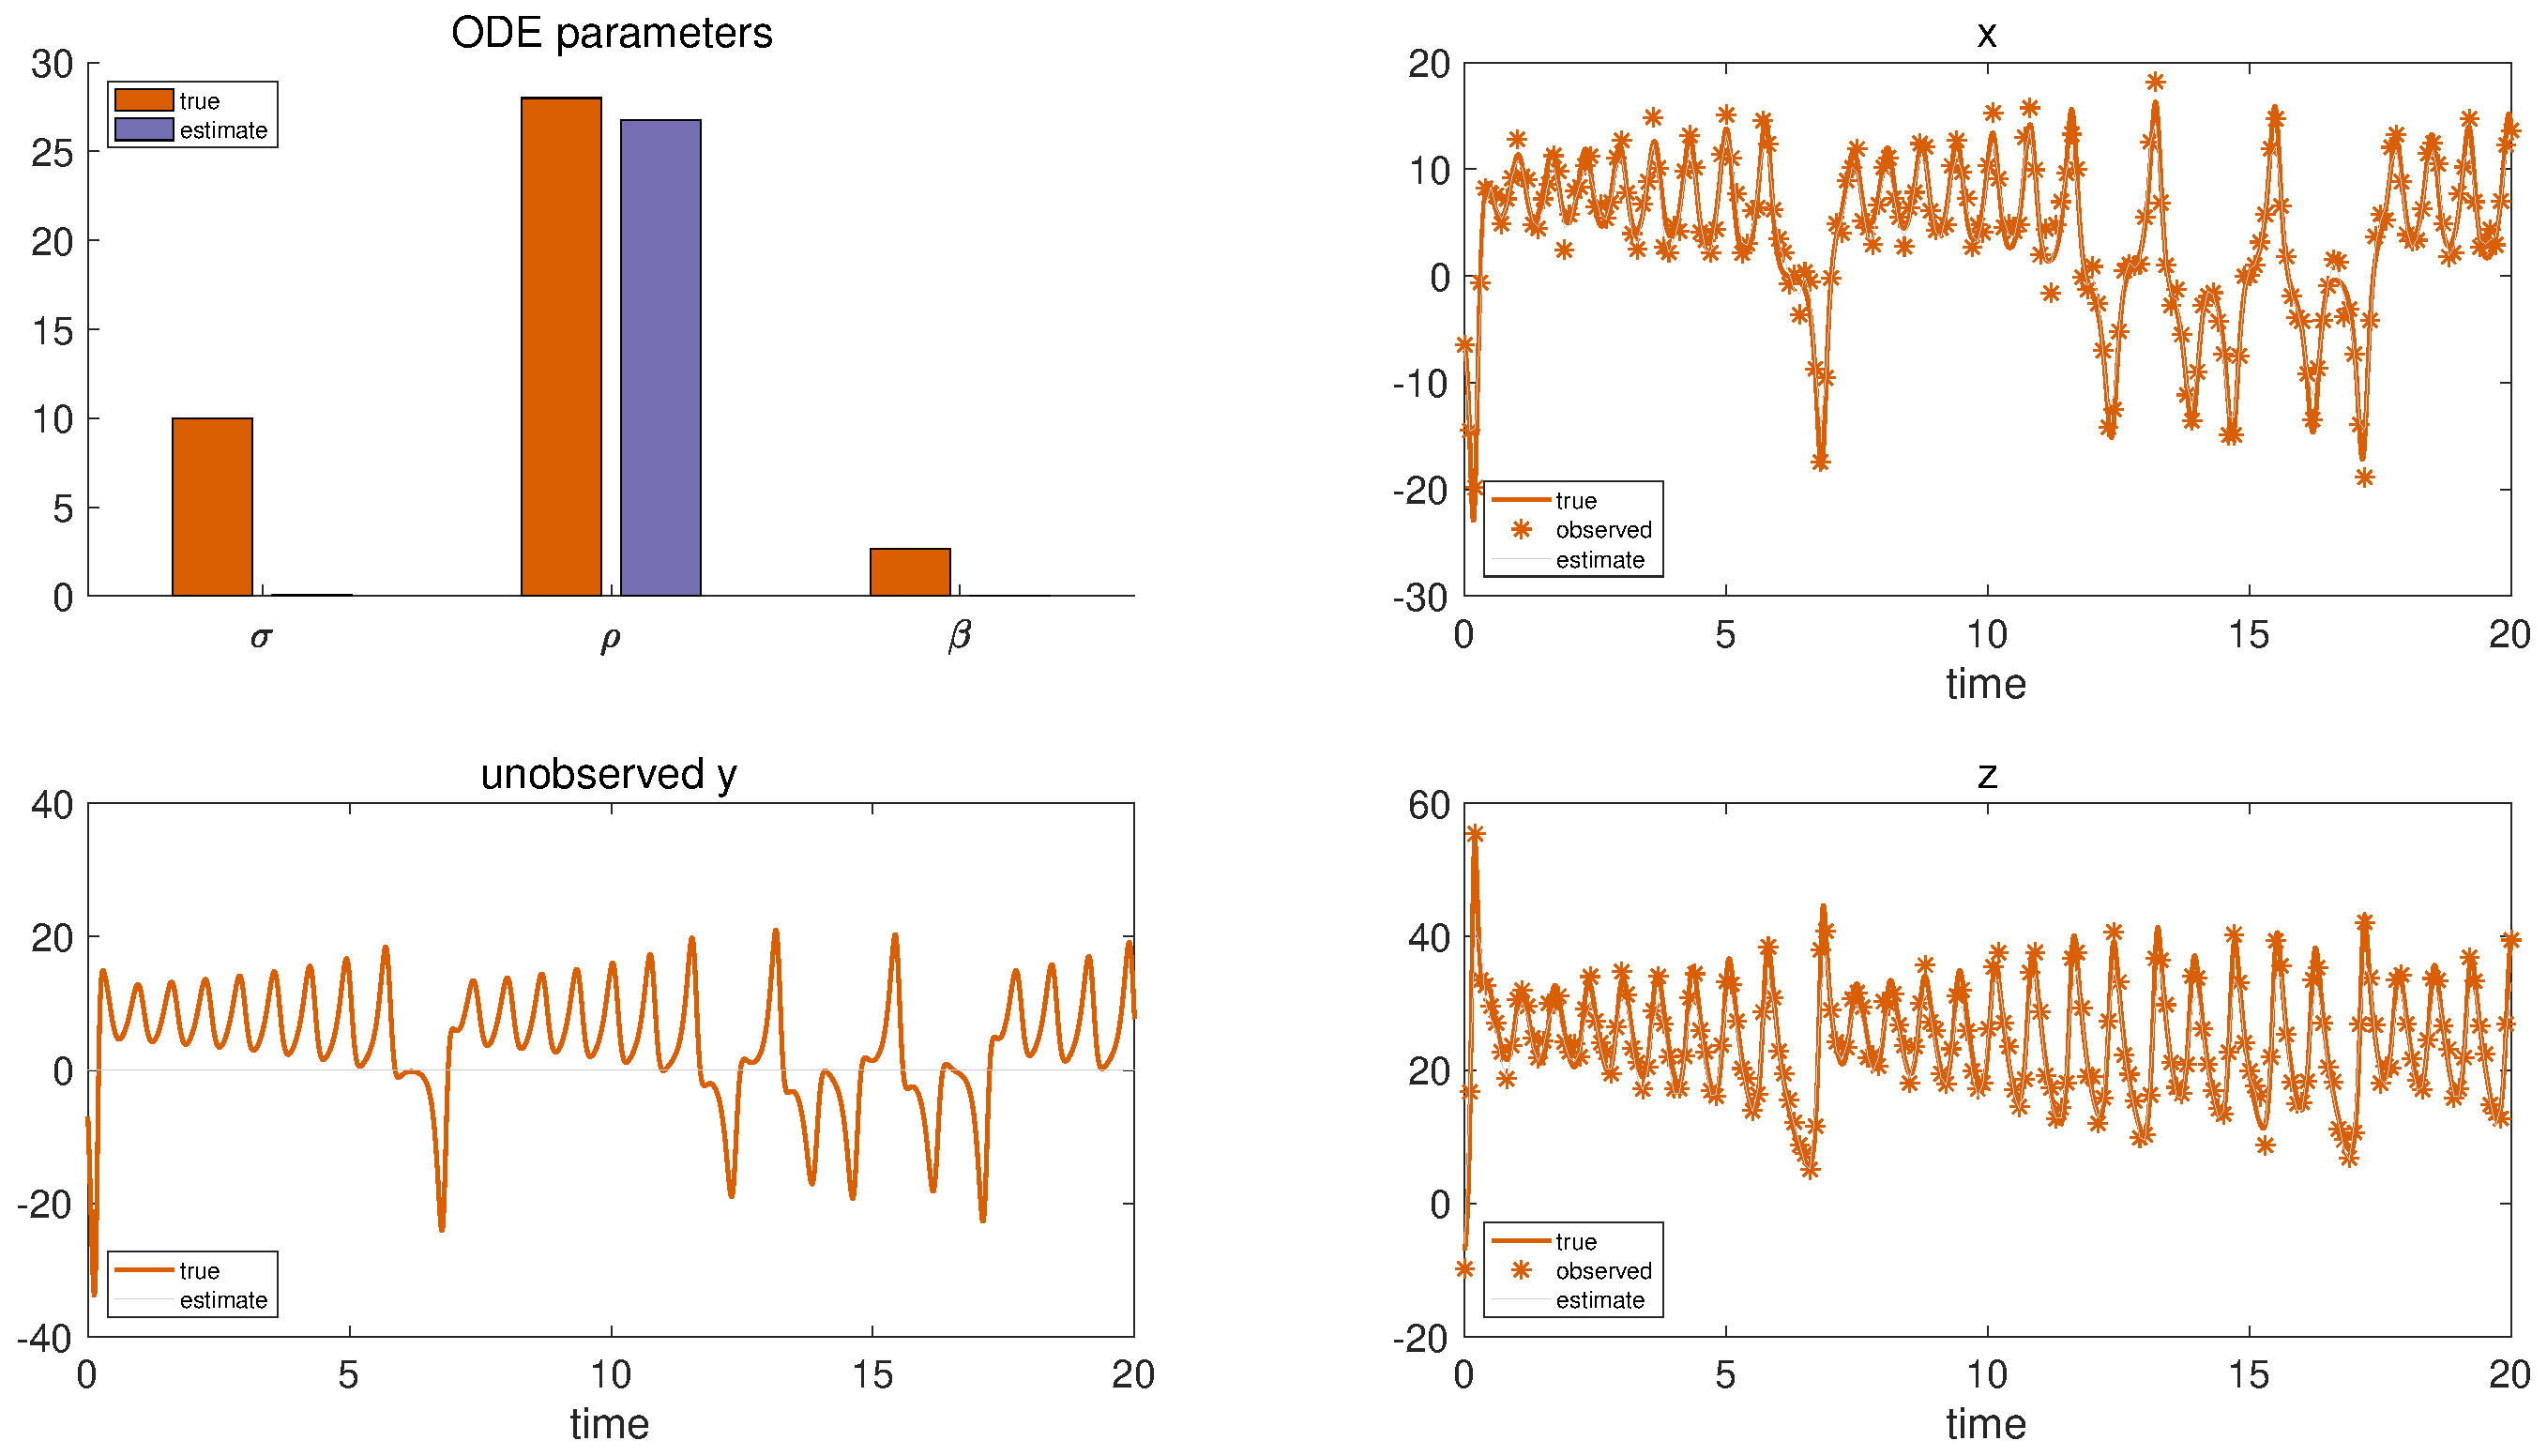
\includegraphics [width=5in]{Lorenz_attractor_4_05.eps}

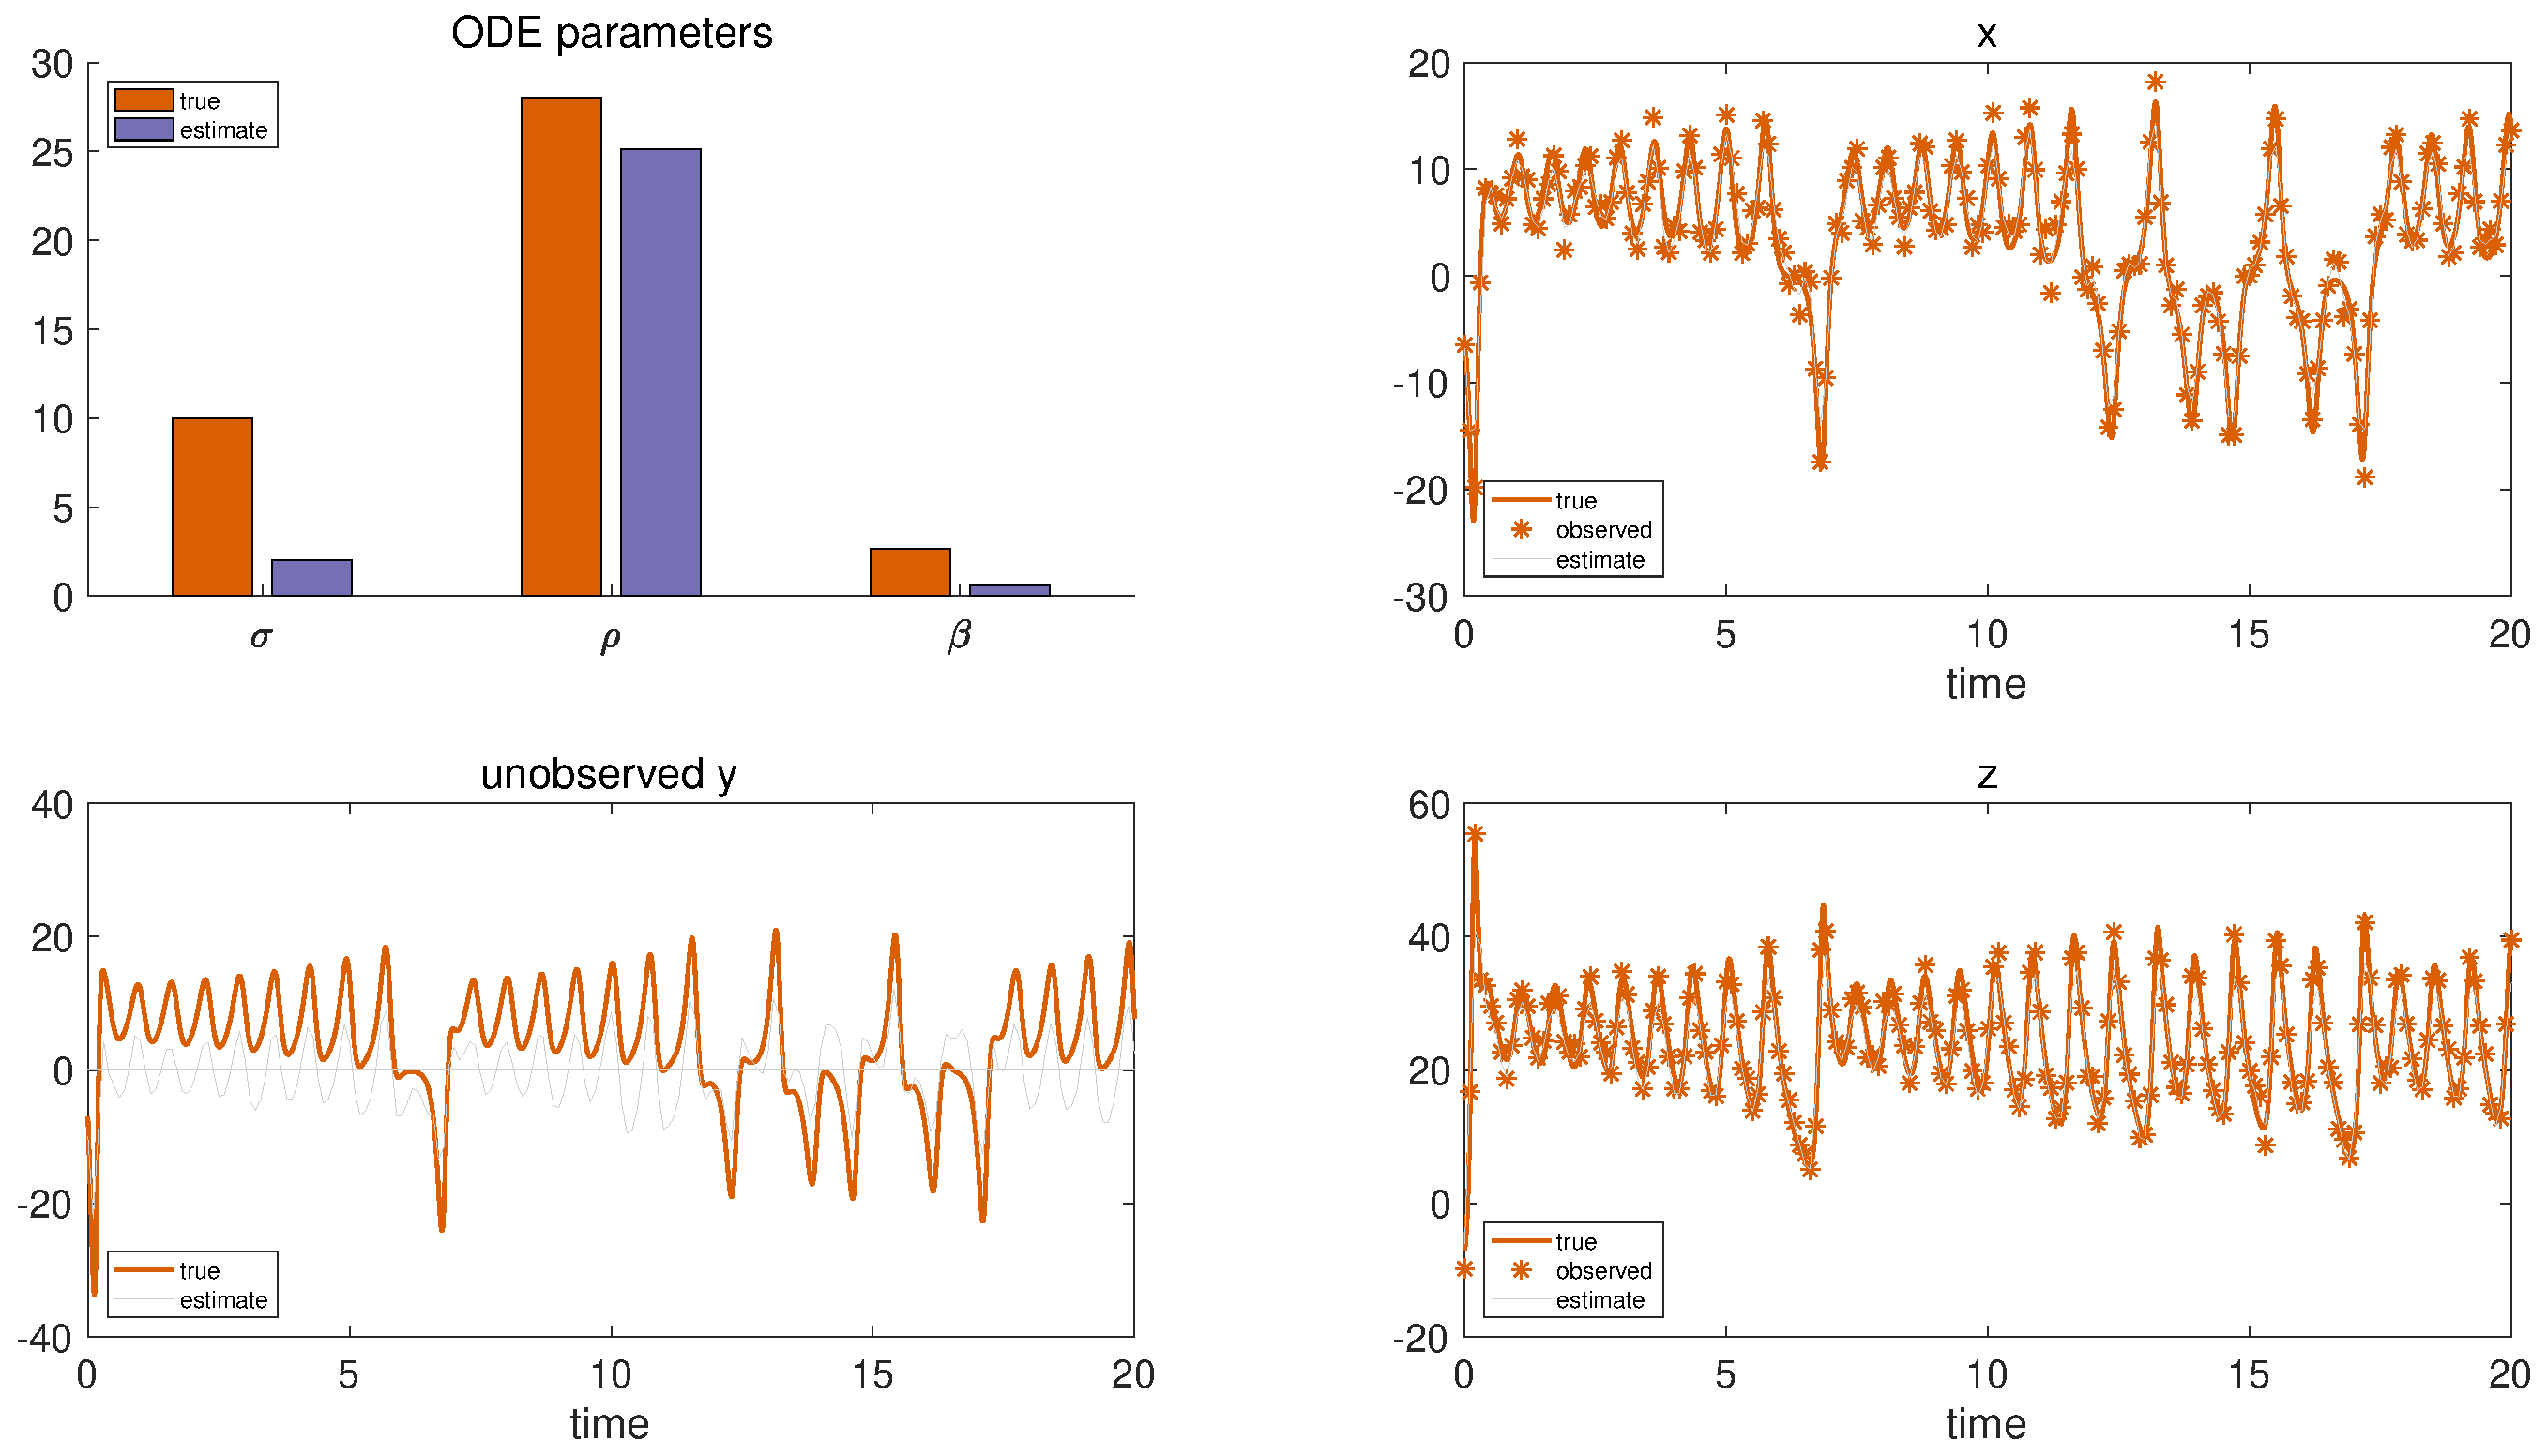
\includegraphics [width=5in]{Lorenz_attractor_4_06.eps}

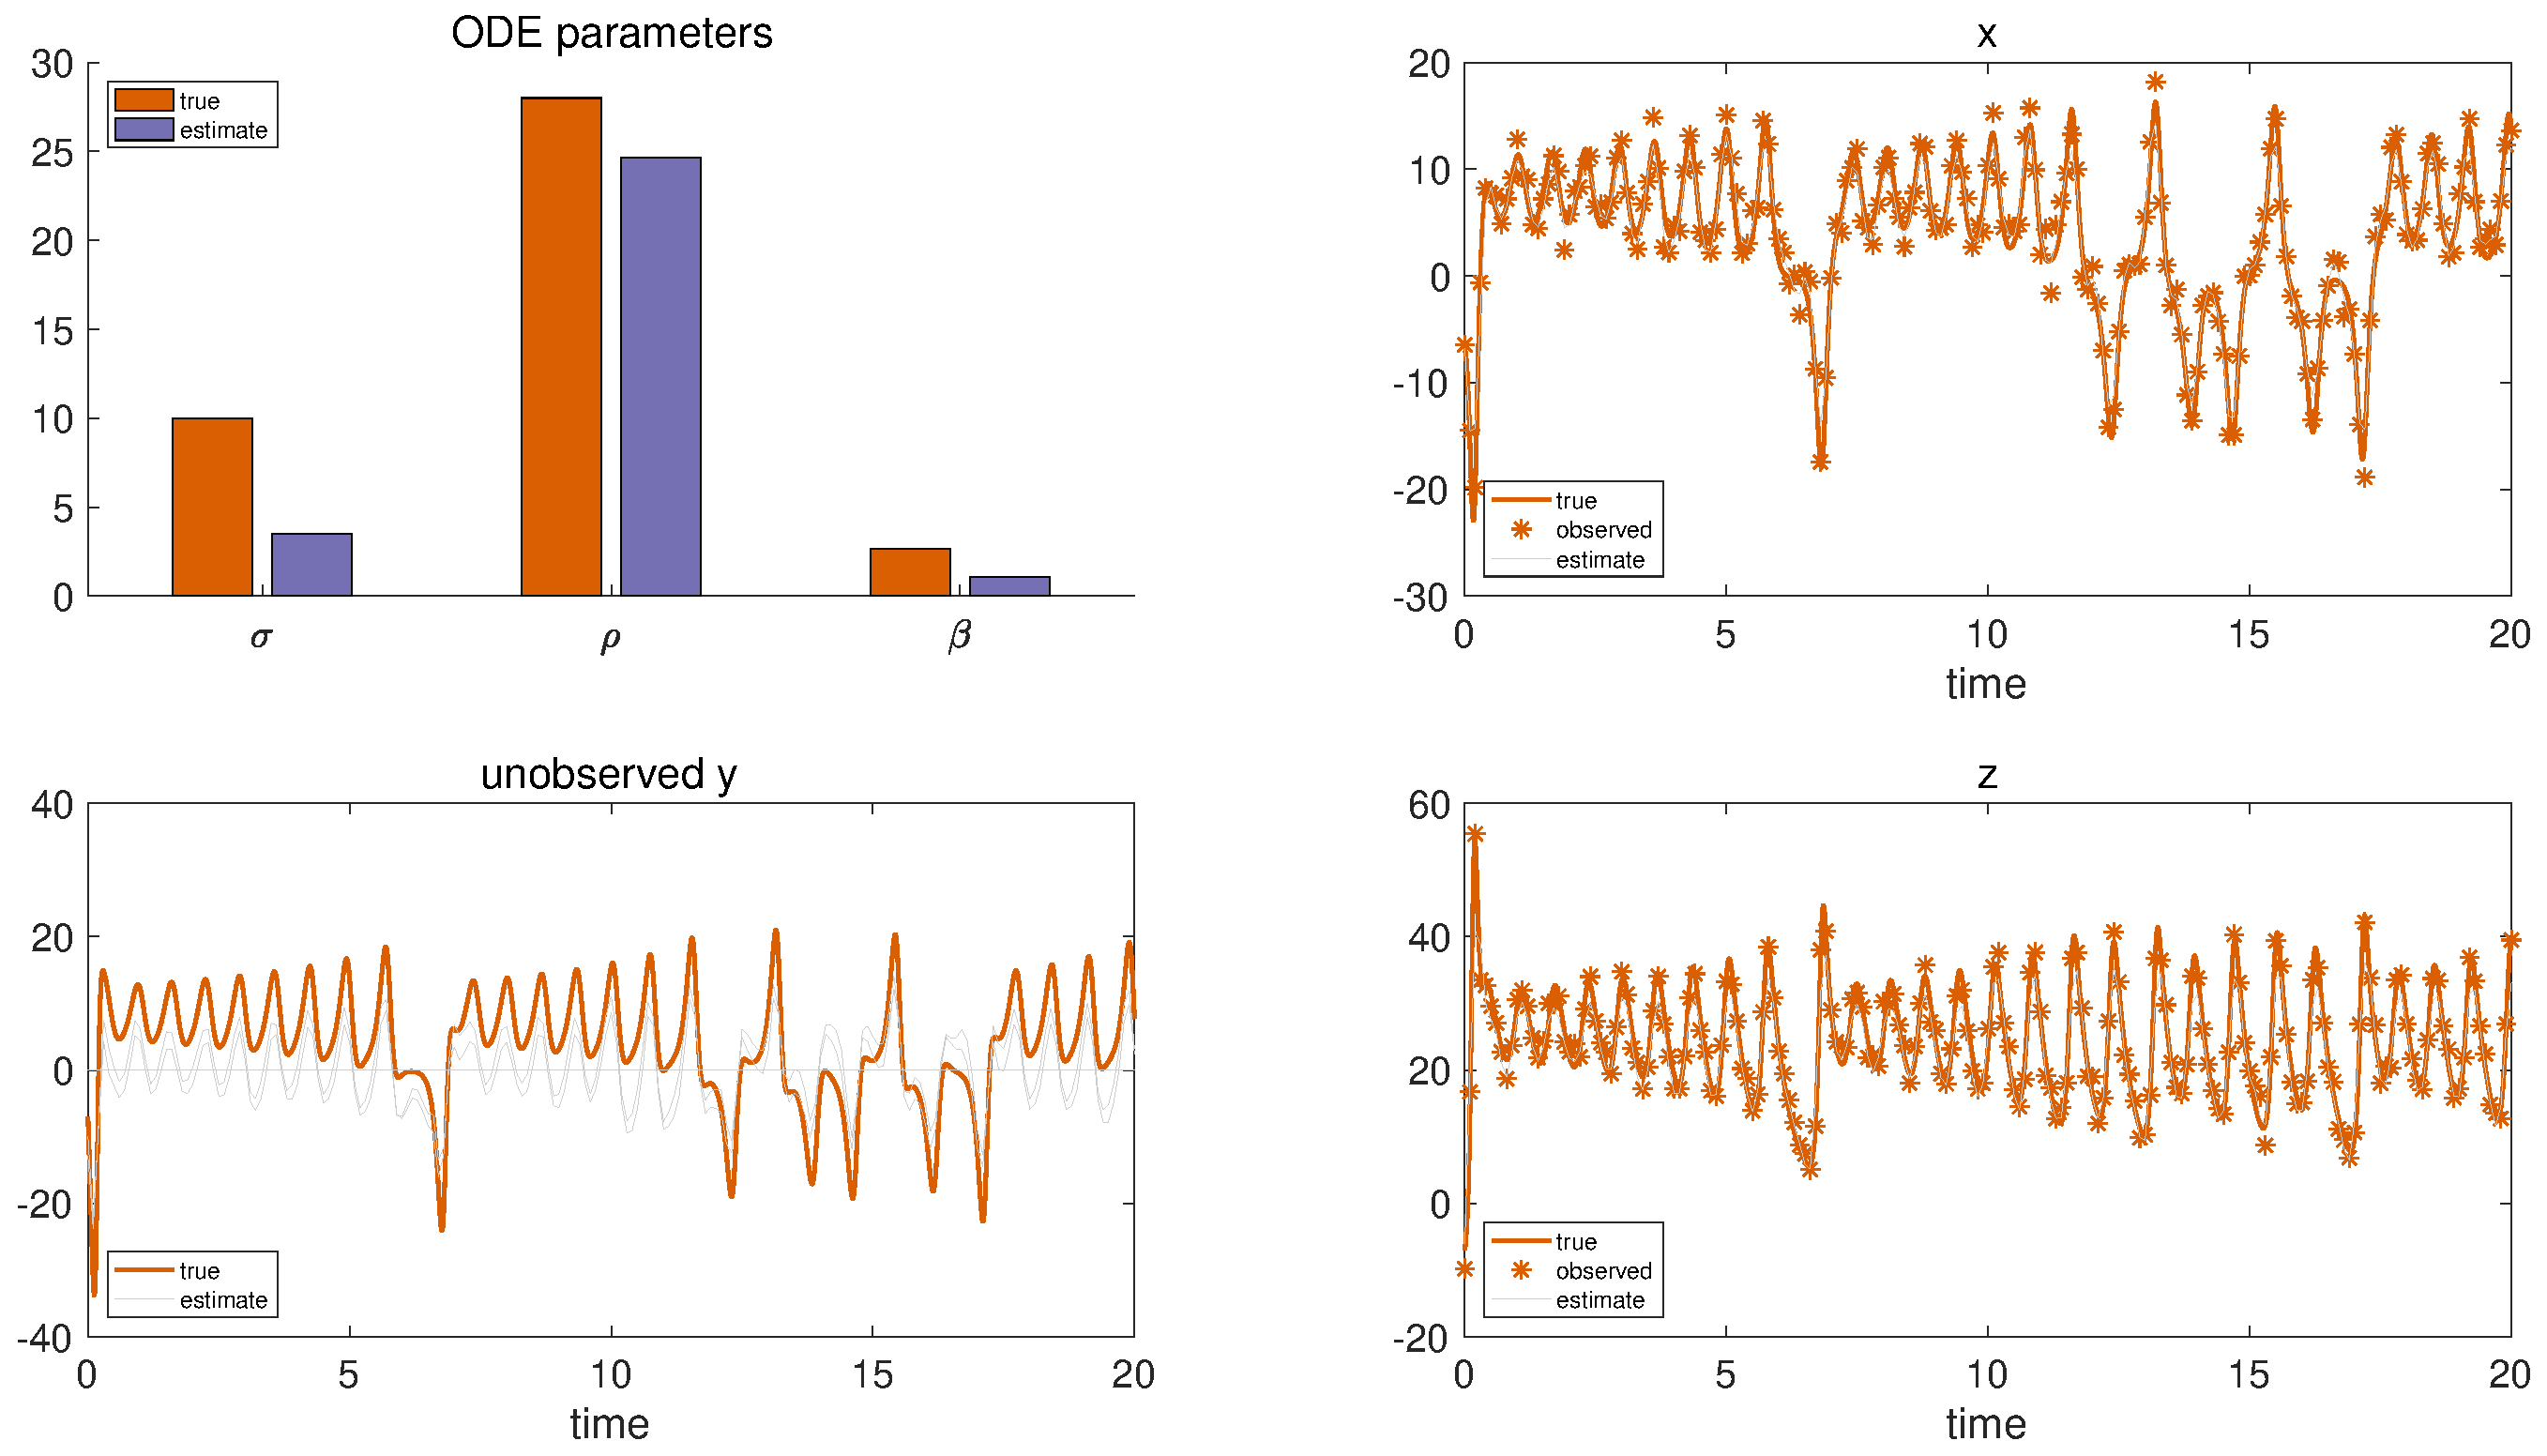
\includegraphics [width=5in]{Lorenz_attractor_4_07.eps}

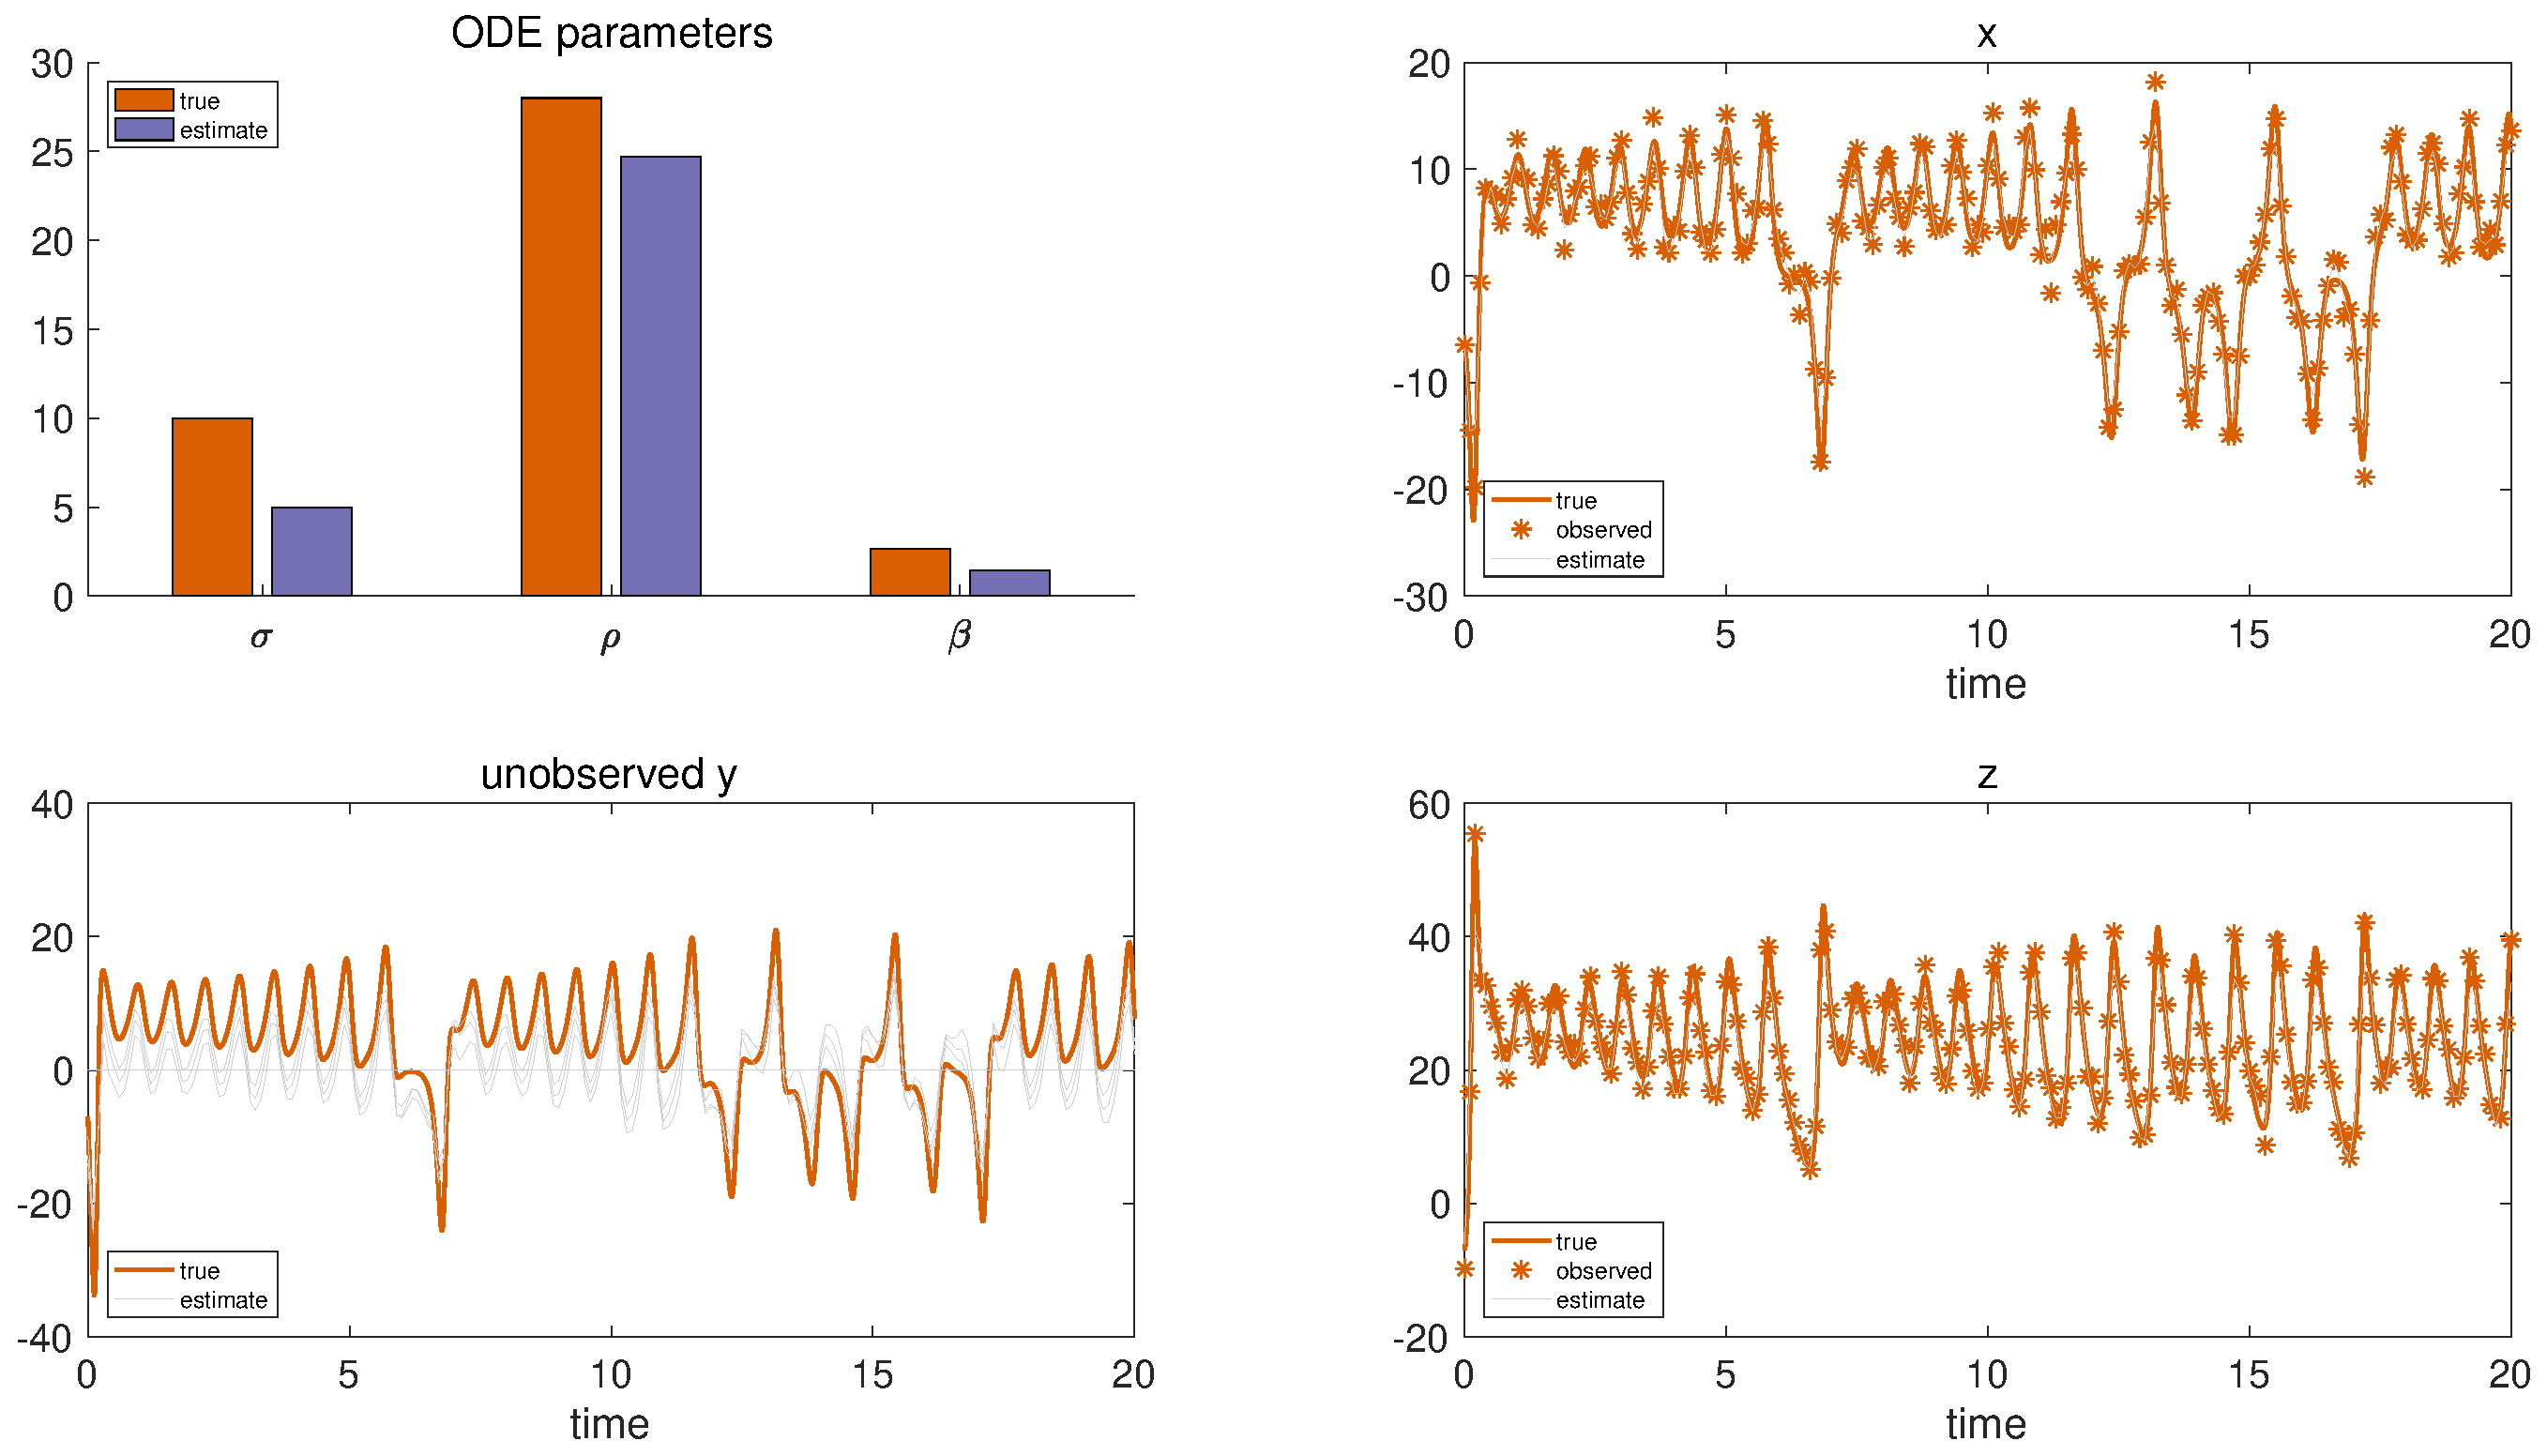
\includegraphics [width=5in]{Lorenz_attractor_4_08.eps}

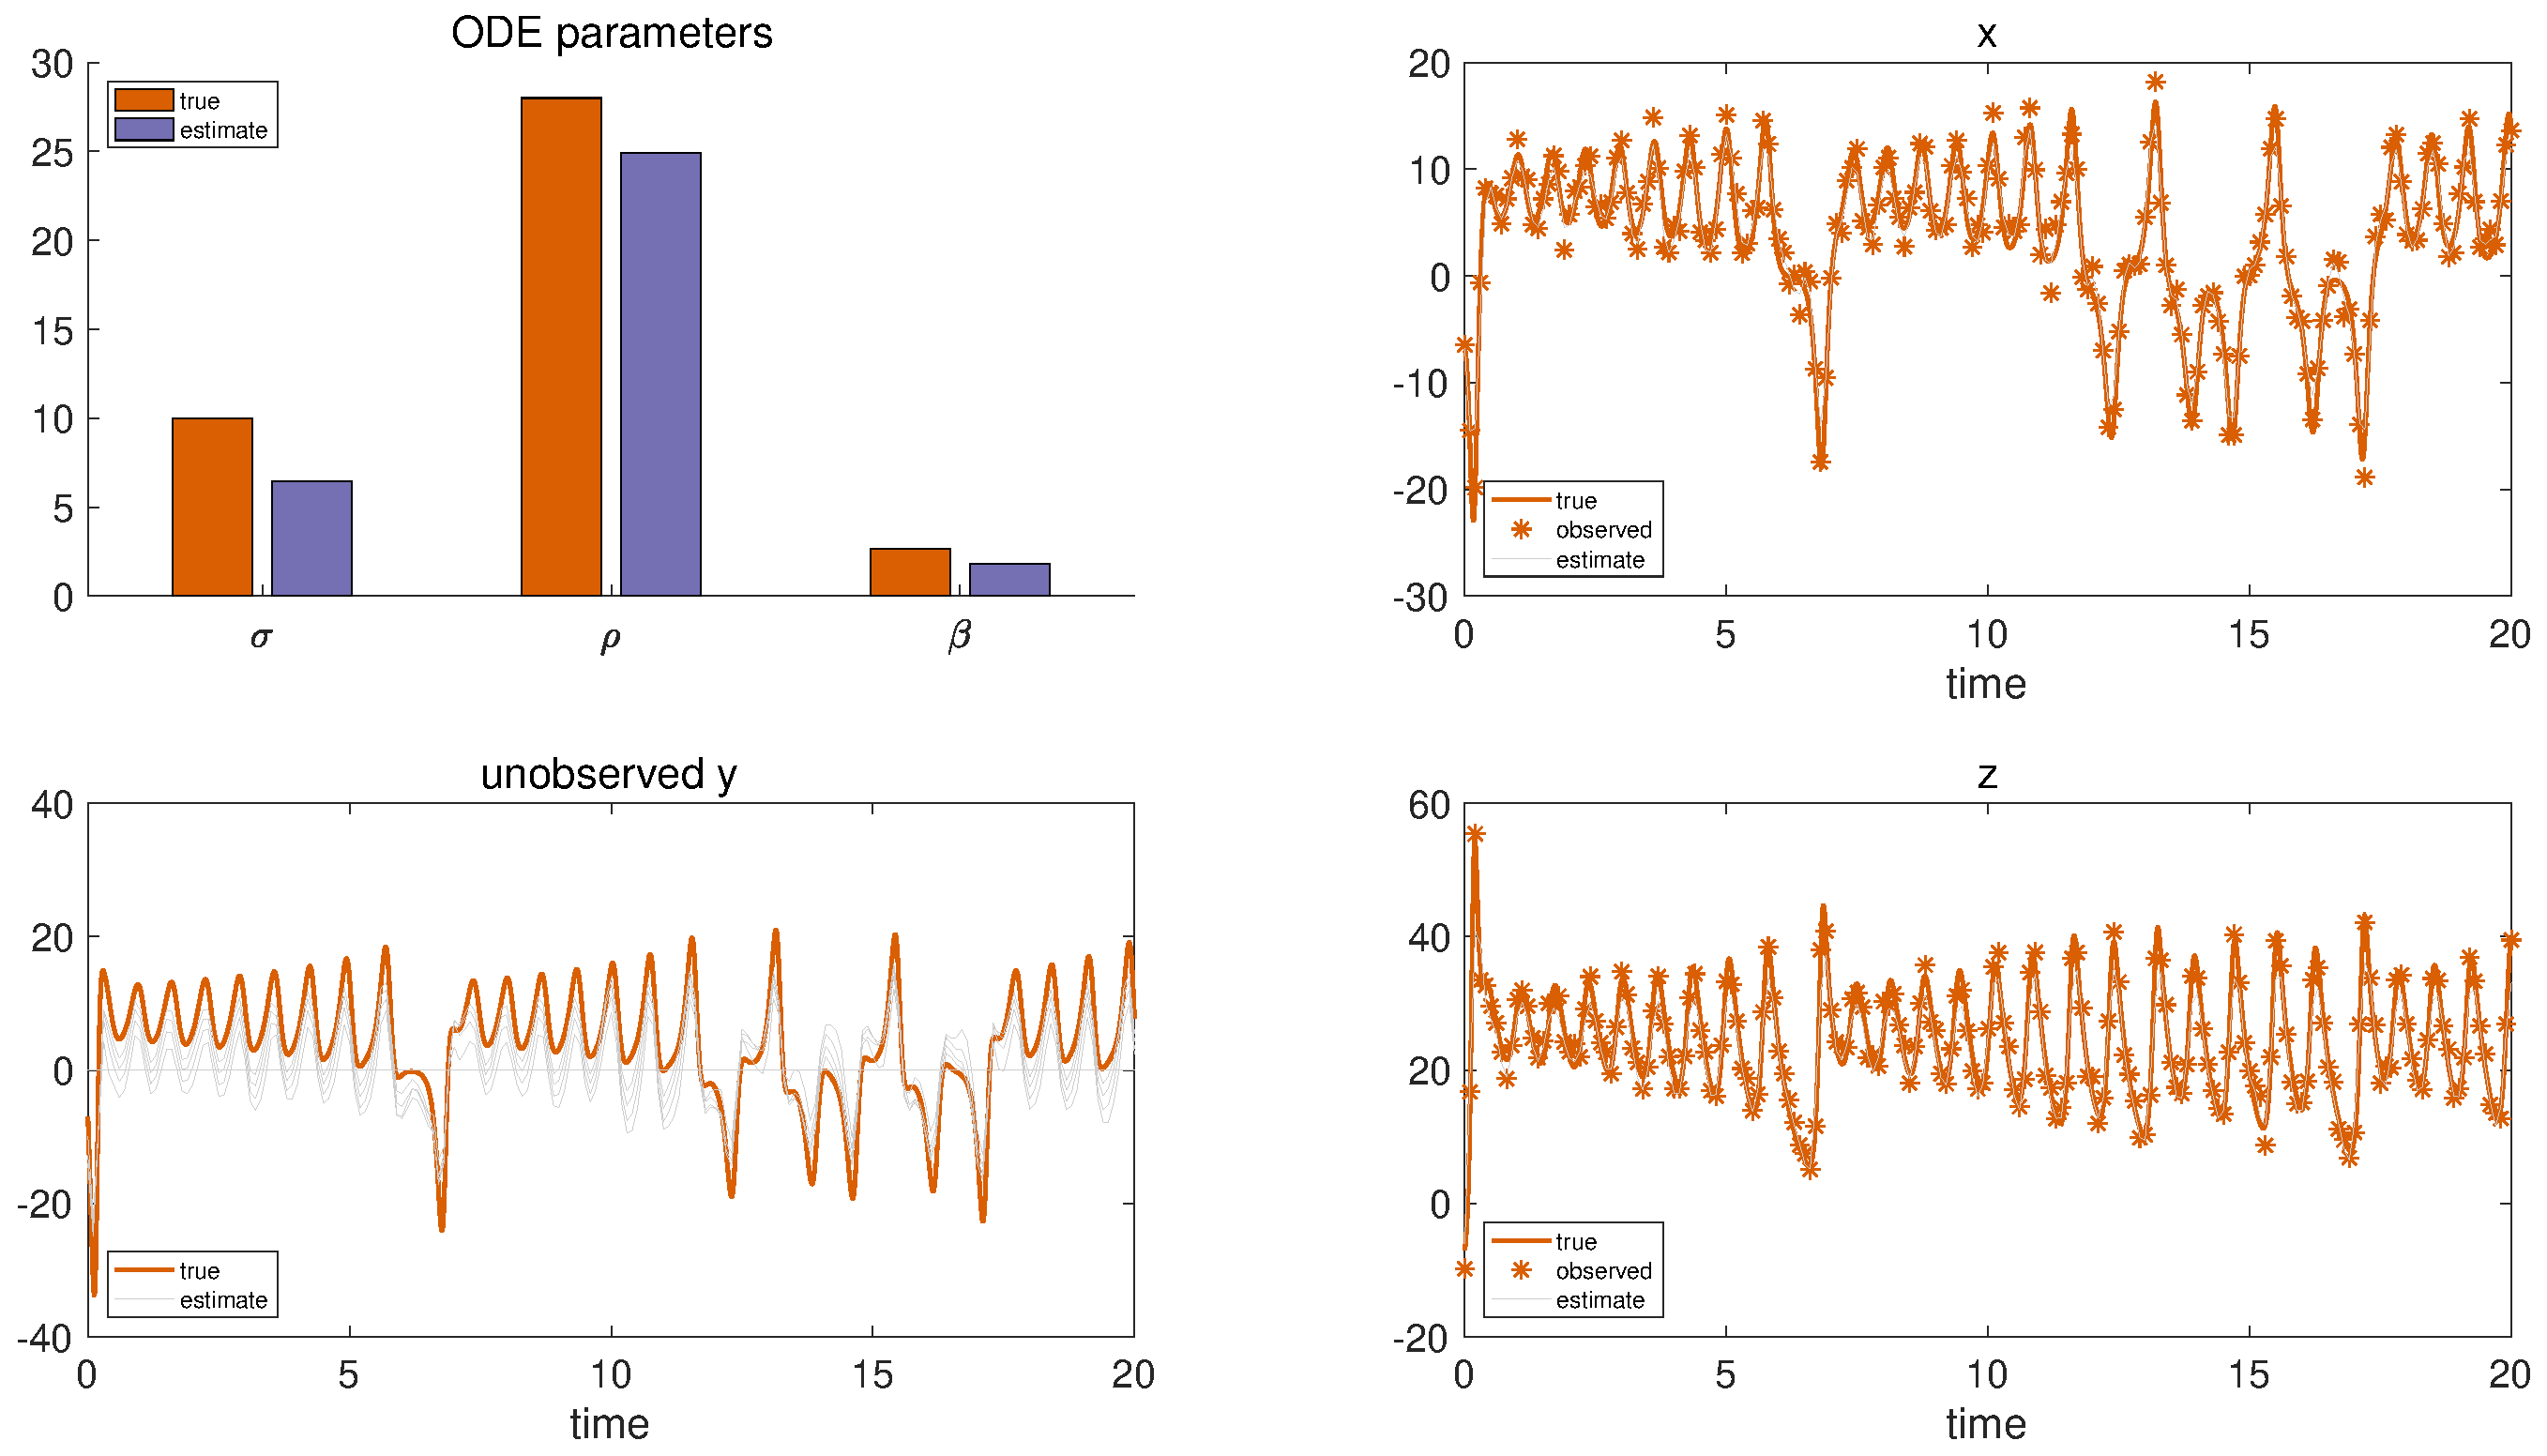
\includegraphics [width=5in]{Lorenz_attractor_4_09.eps}

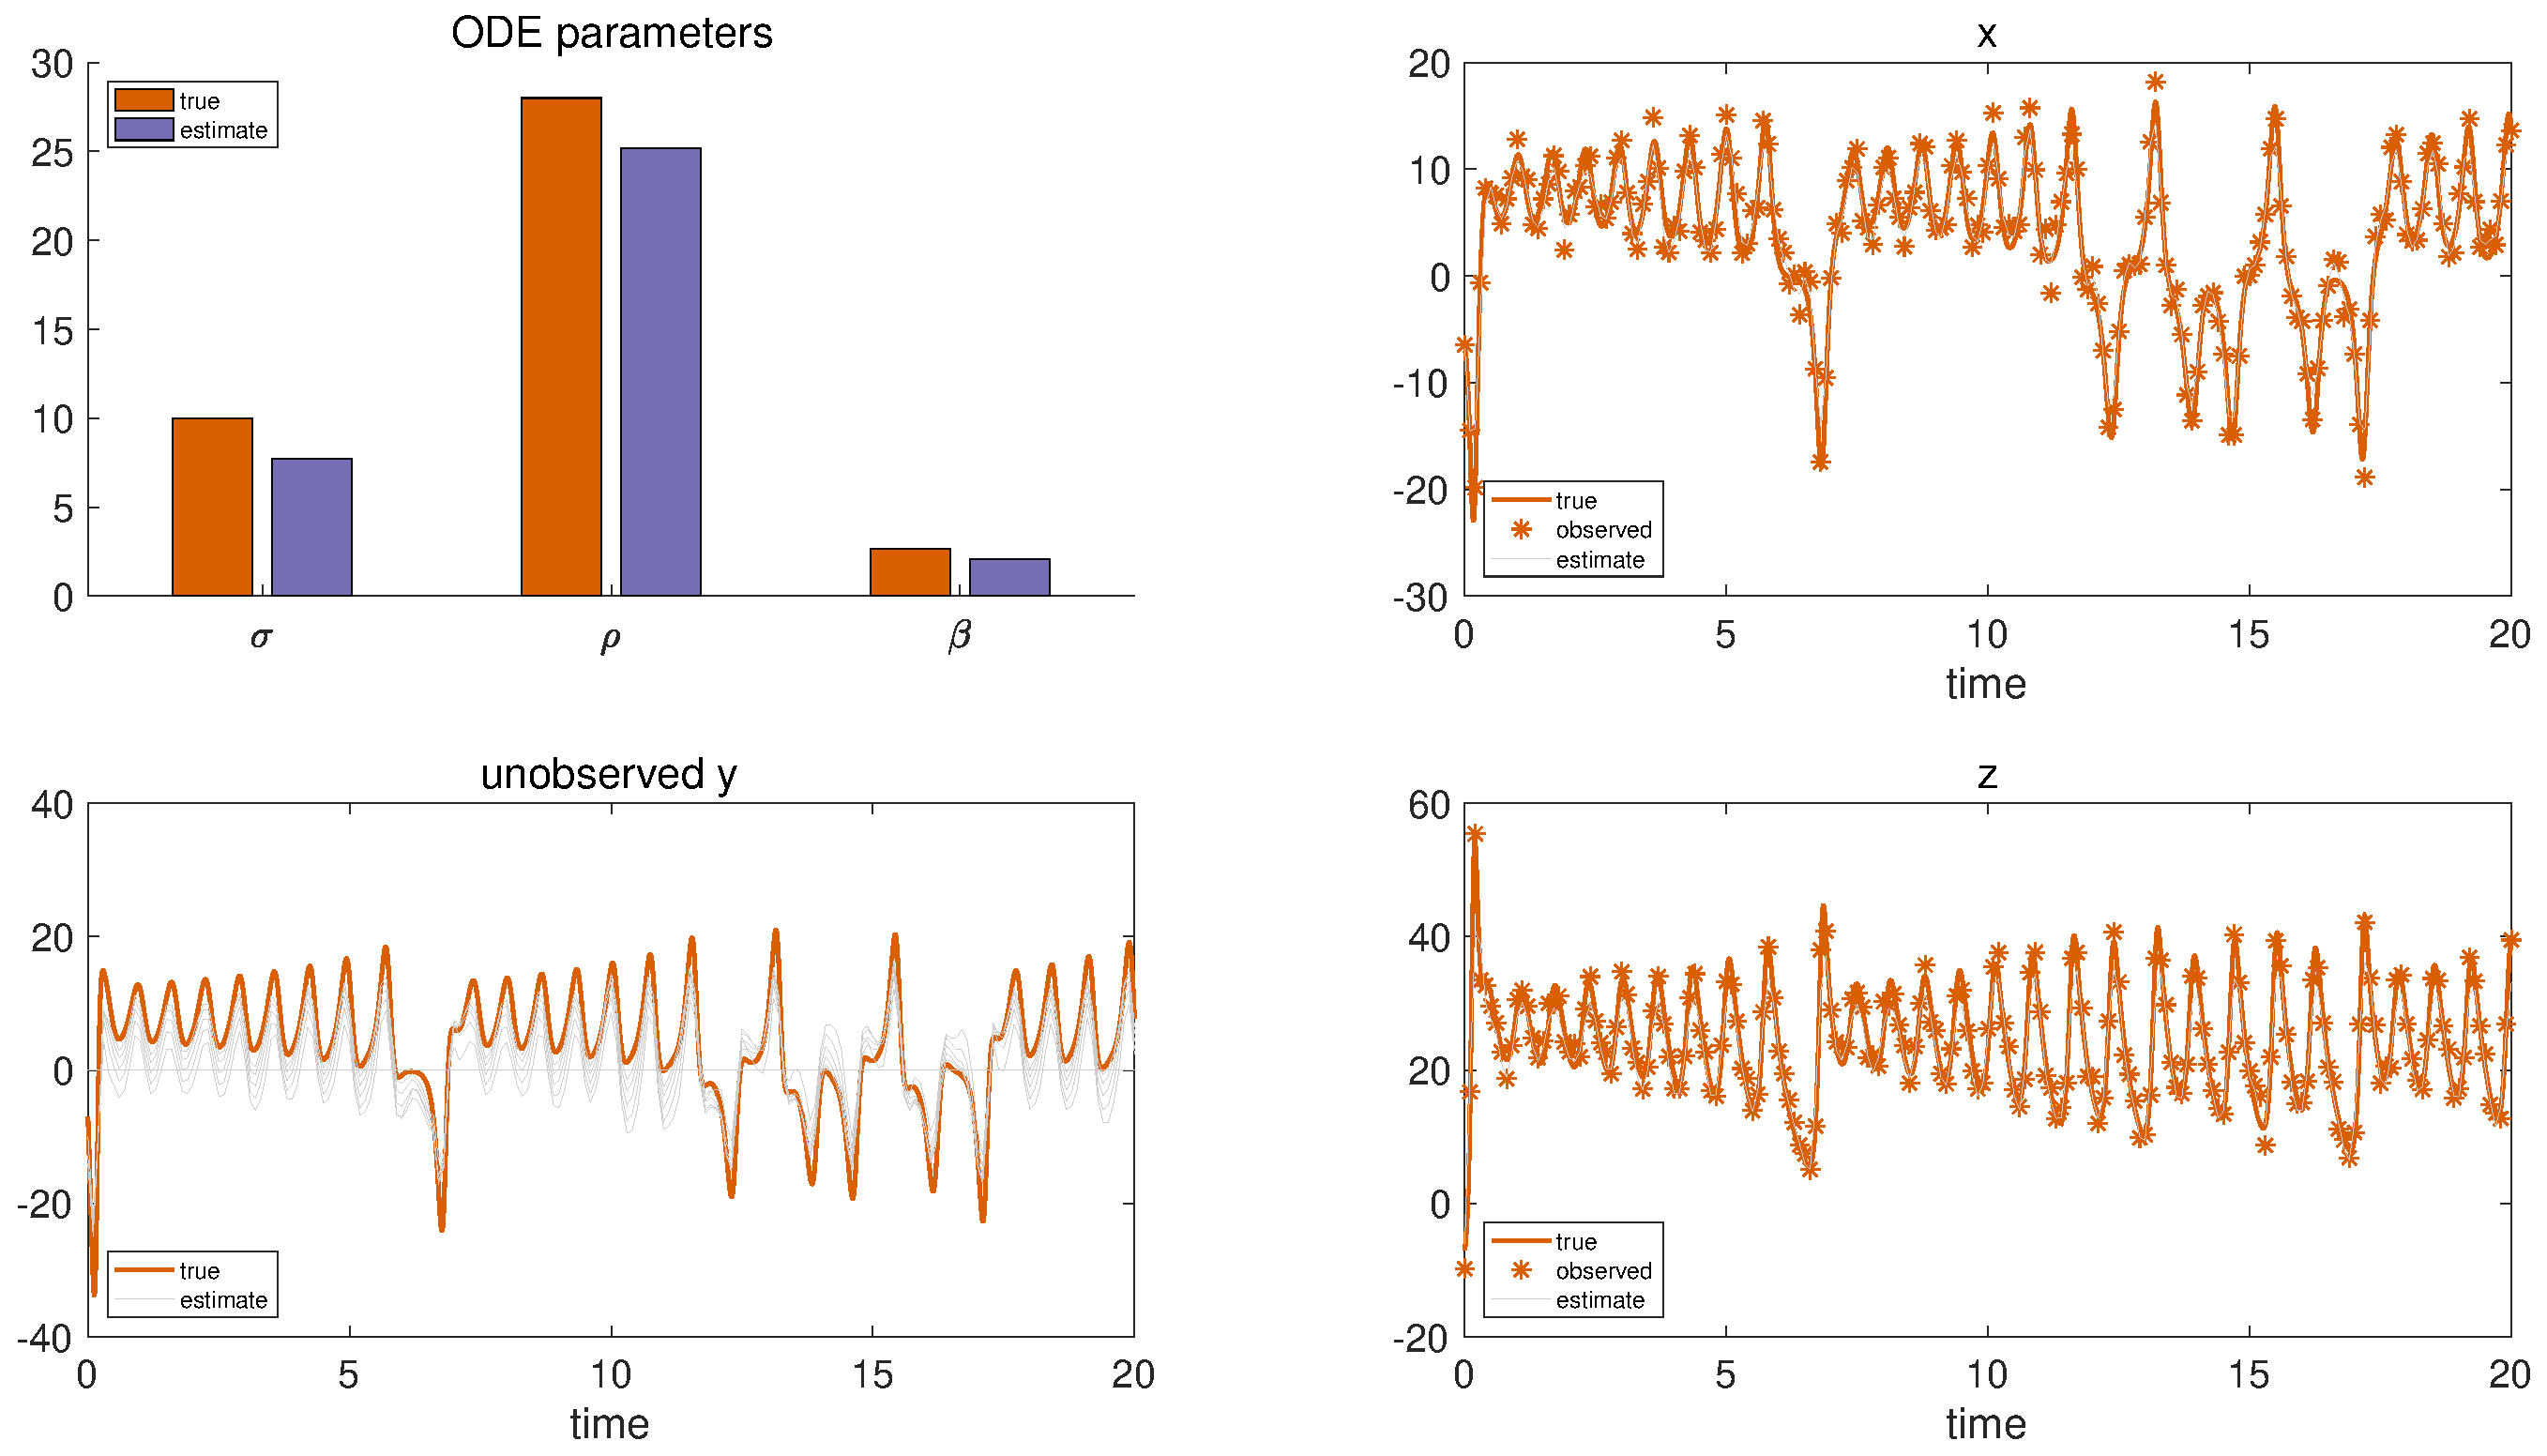
\includegraphics [width=5in]{Lorenz_attractor_4_10.eps}

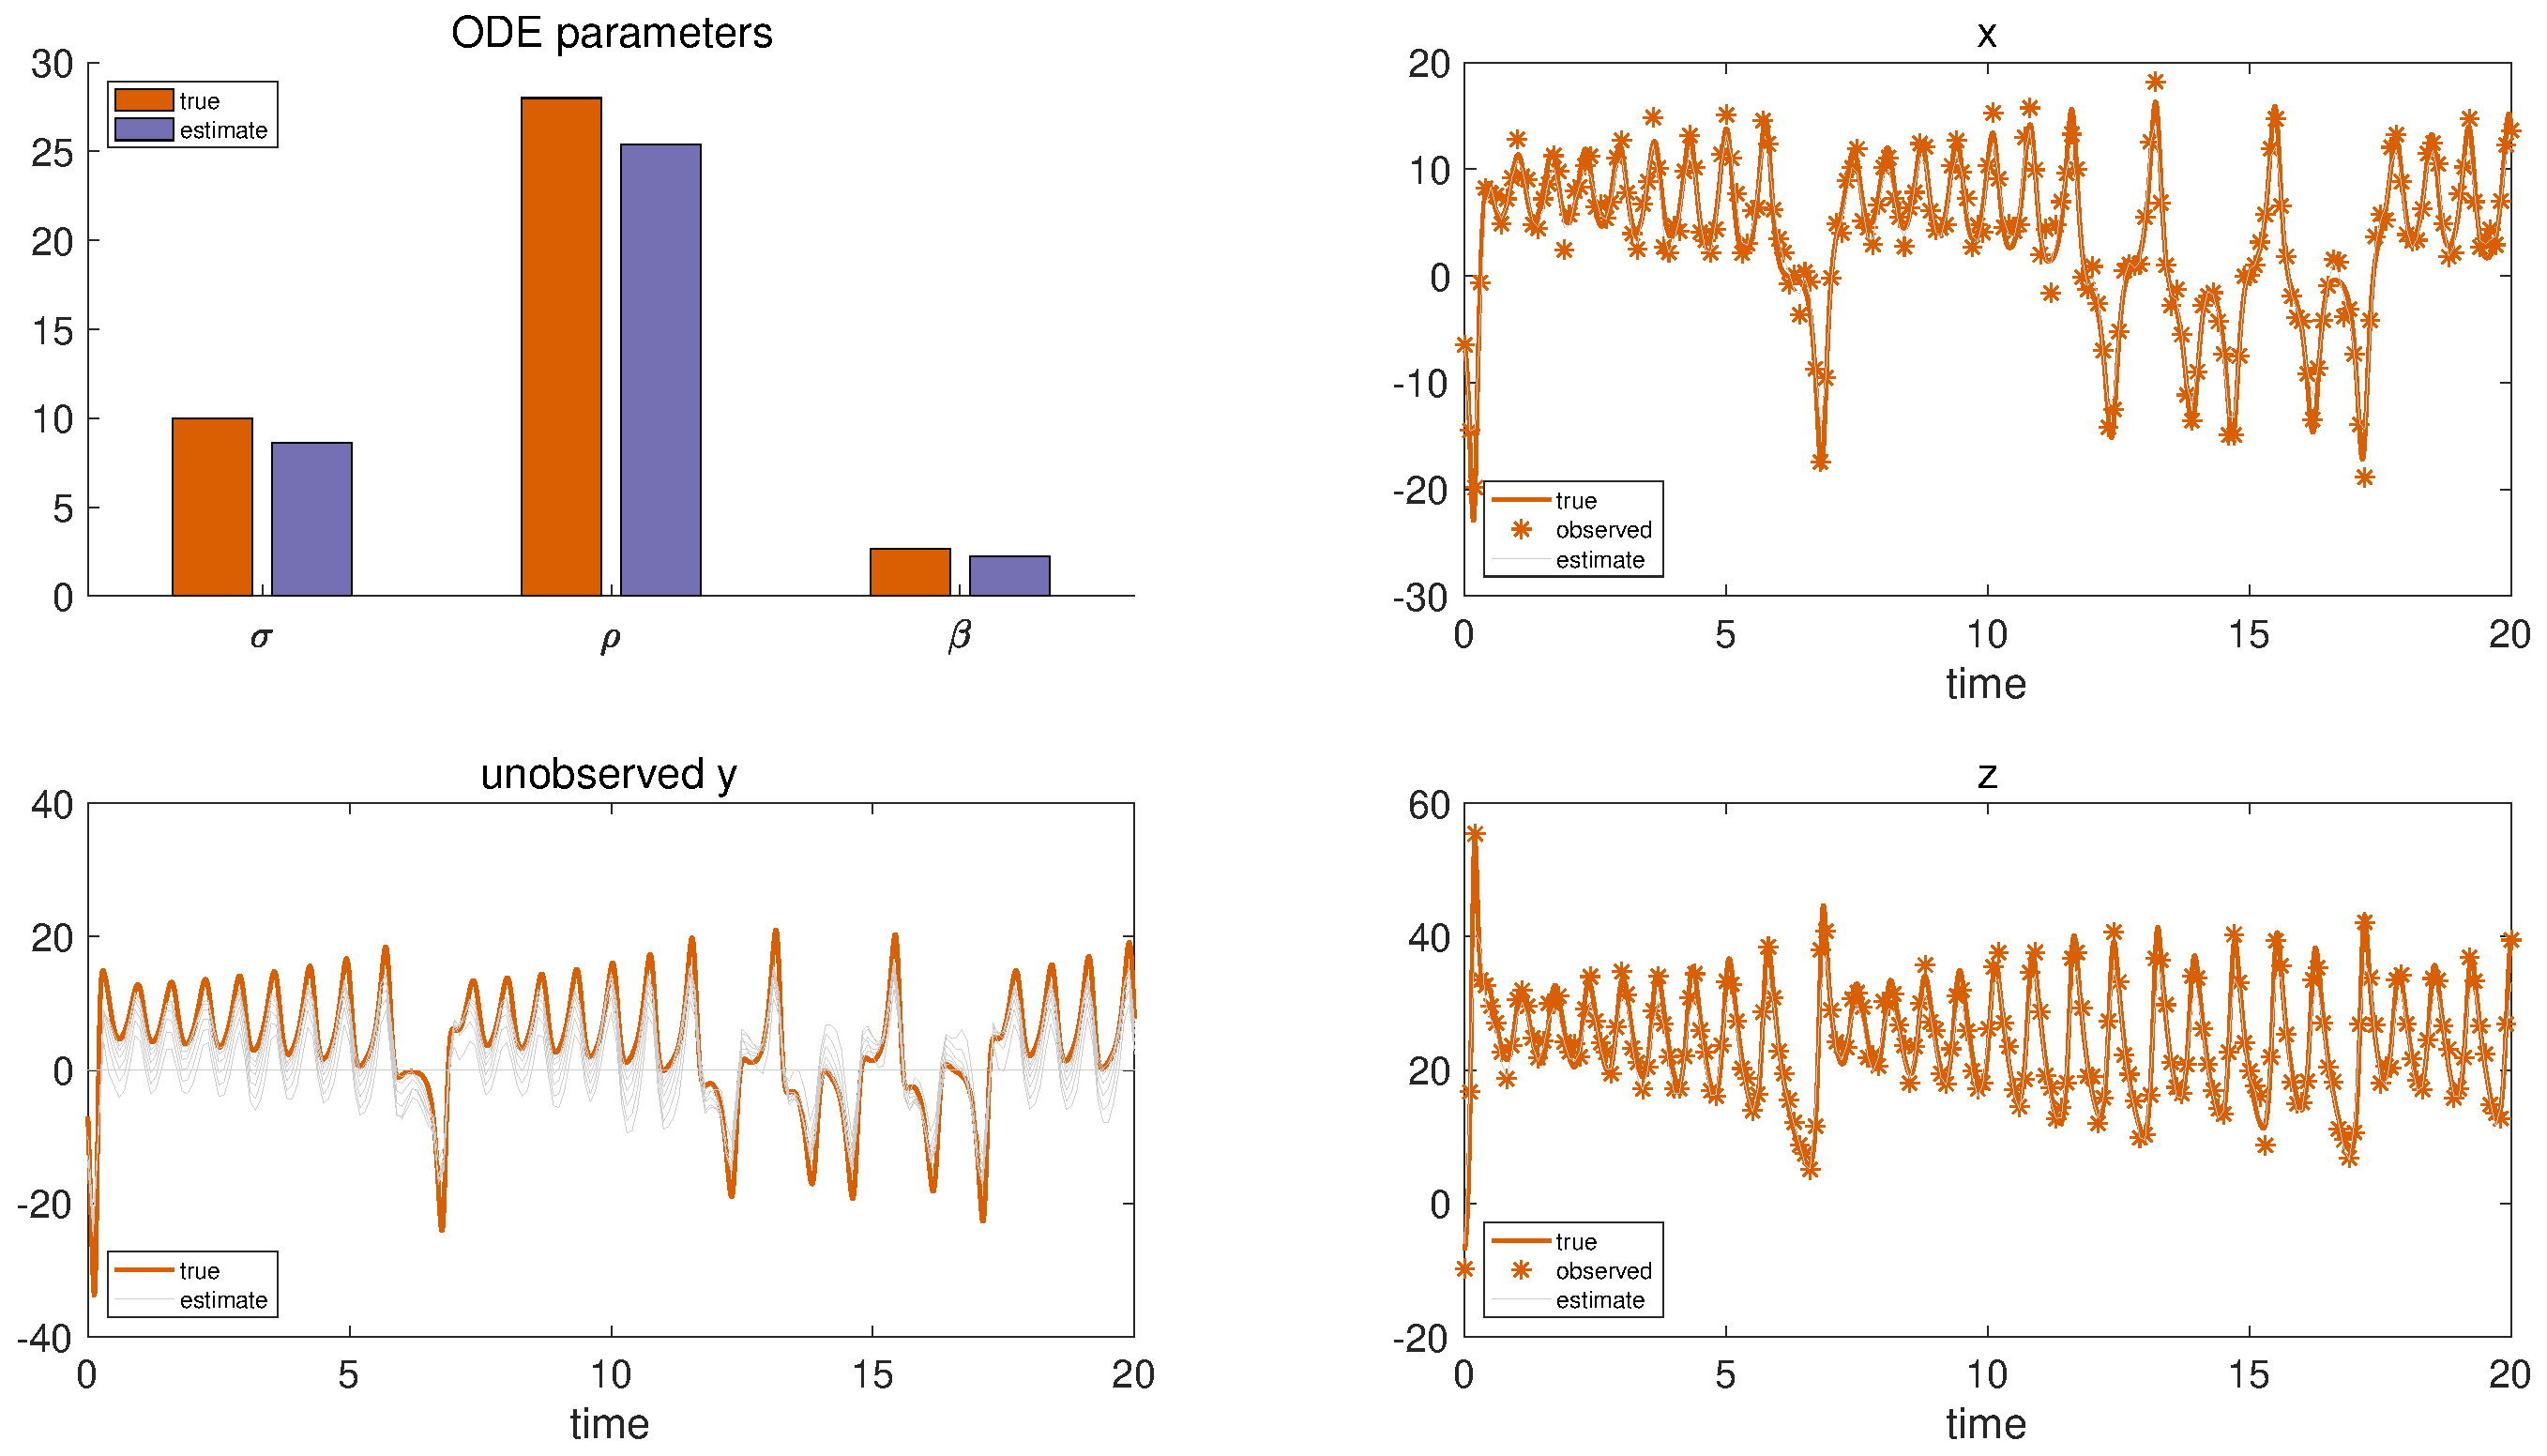
\includegraphics [width=5in]{Lorenz_attractor_4_11.eps}

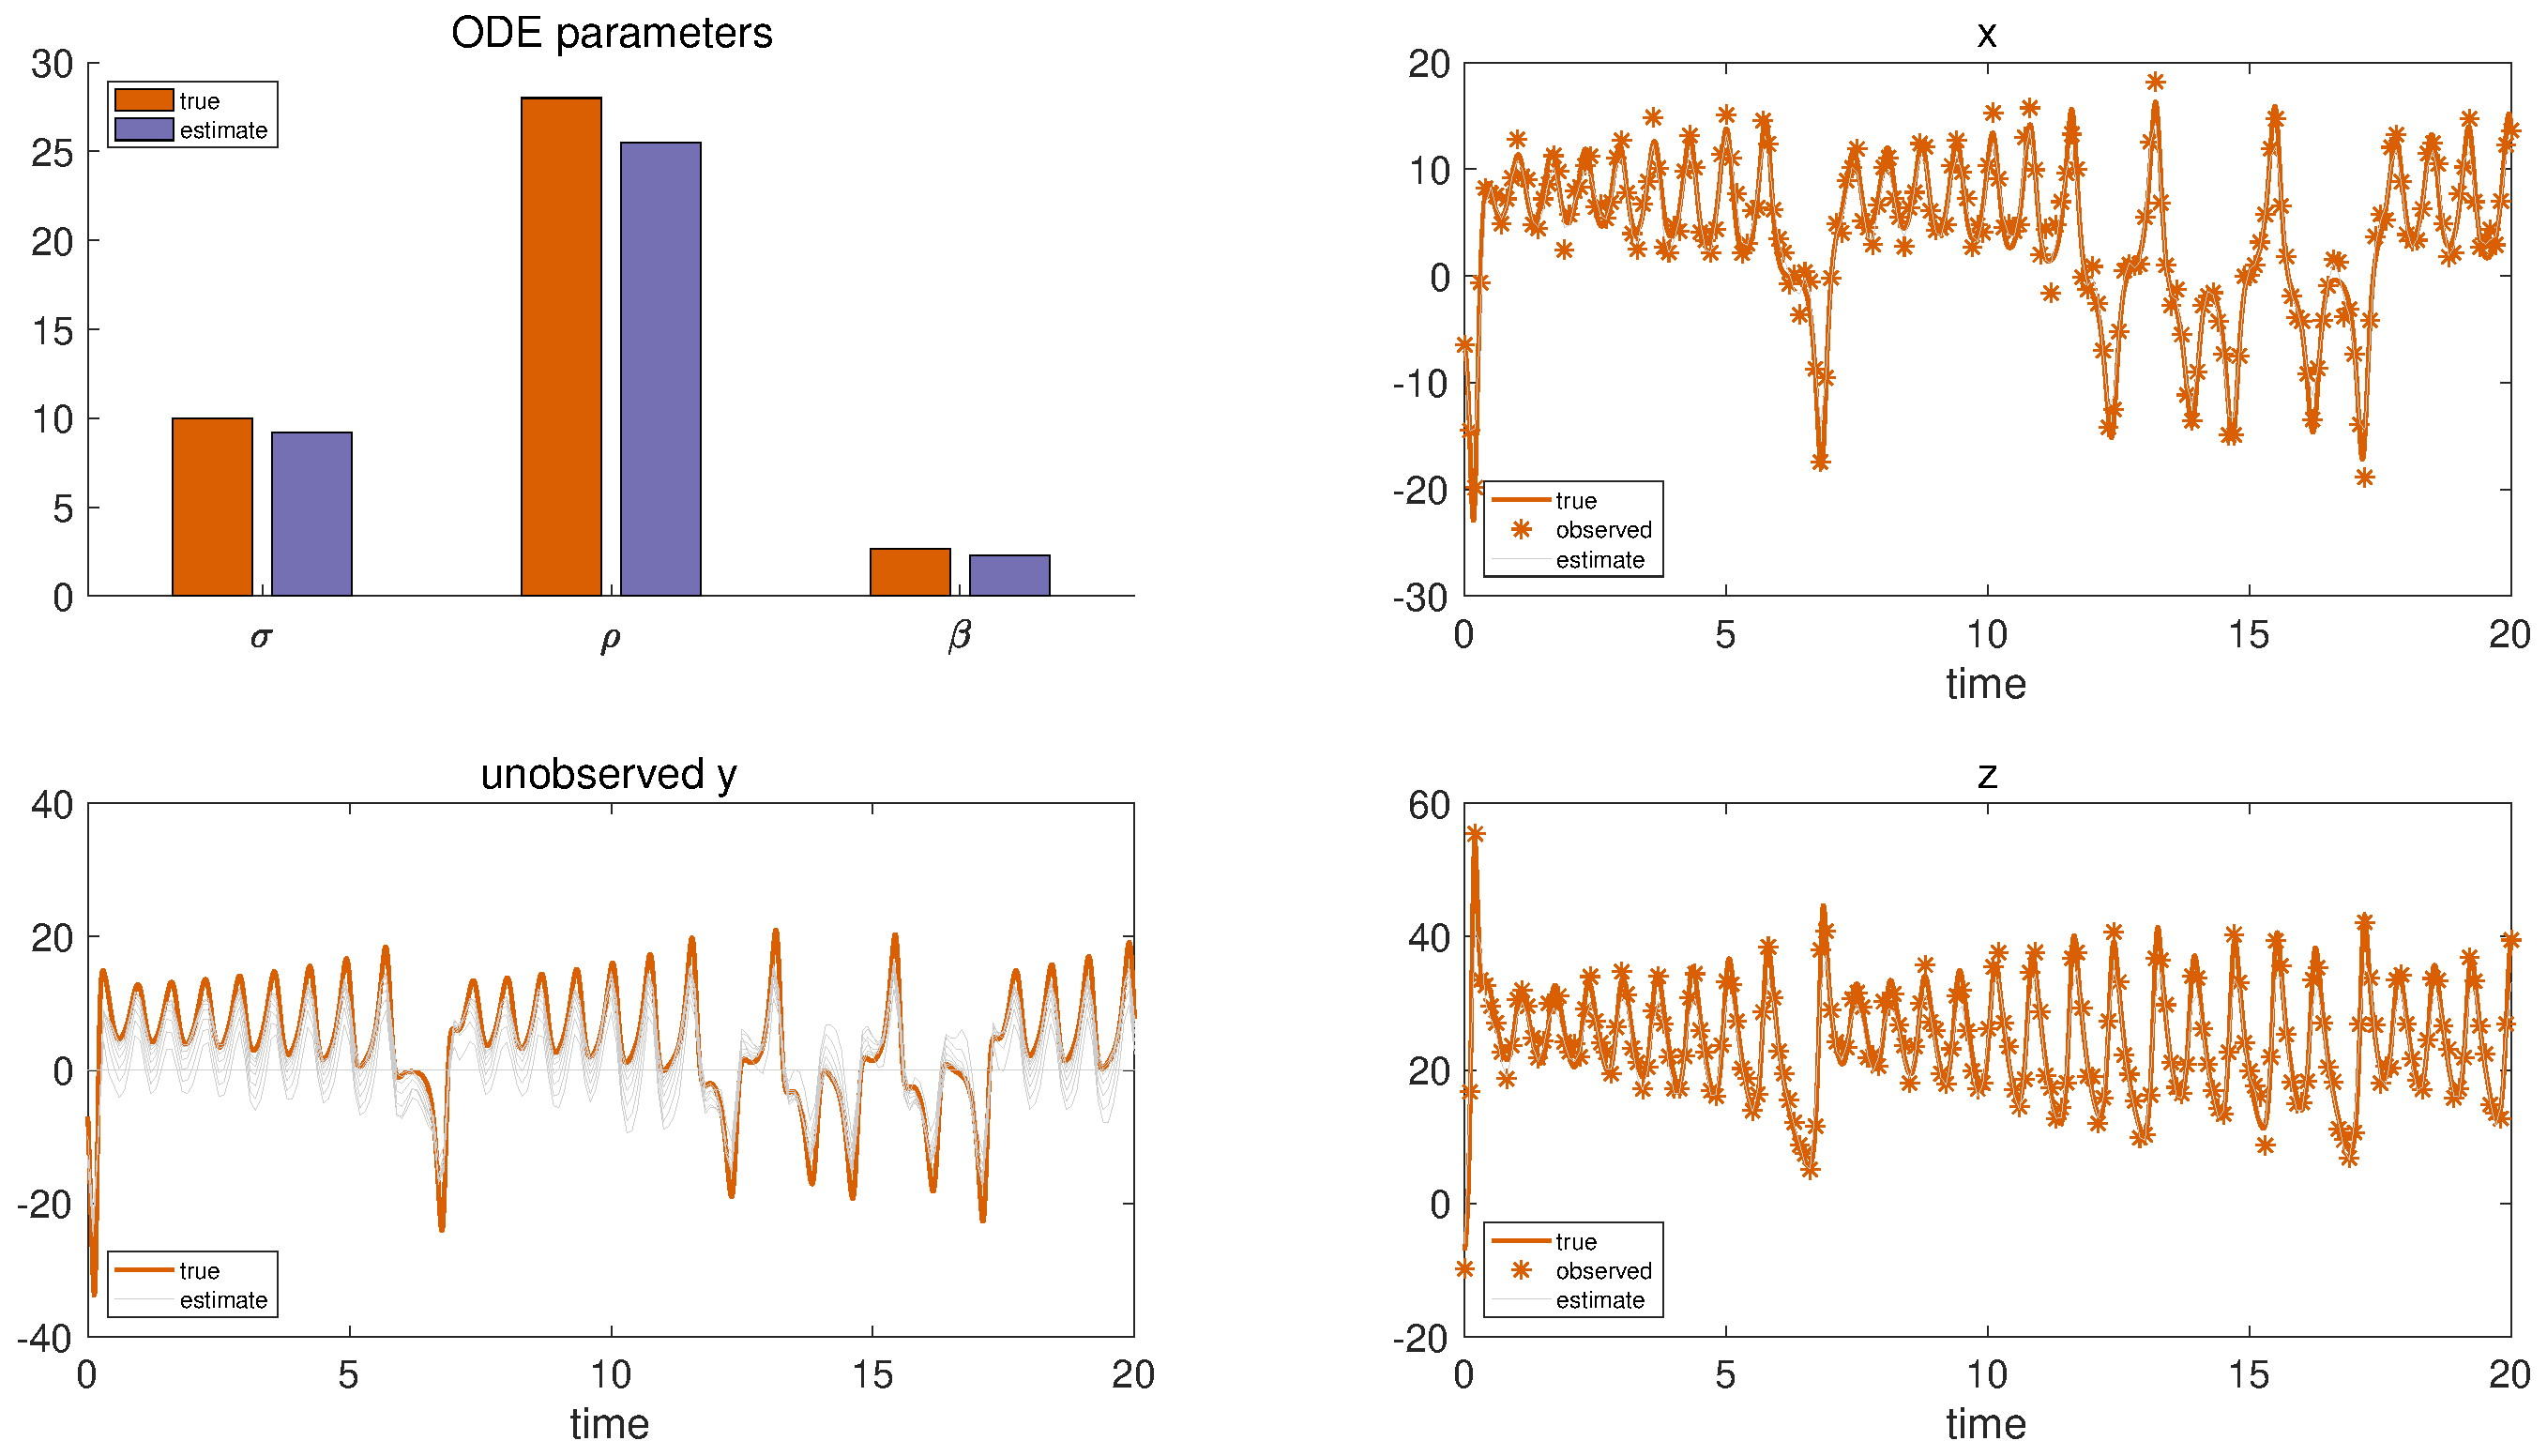
\includegraphics [width=5in]{Lorenz_attractor_4_12.eps}

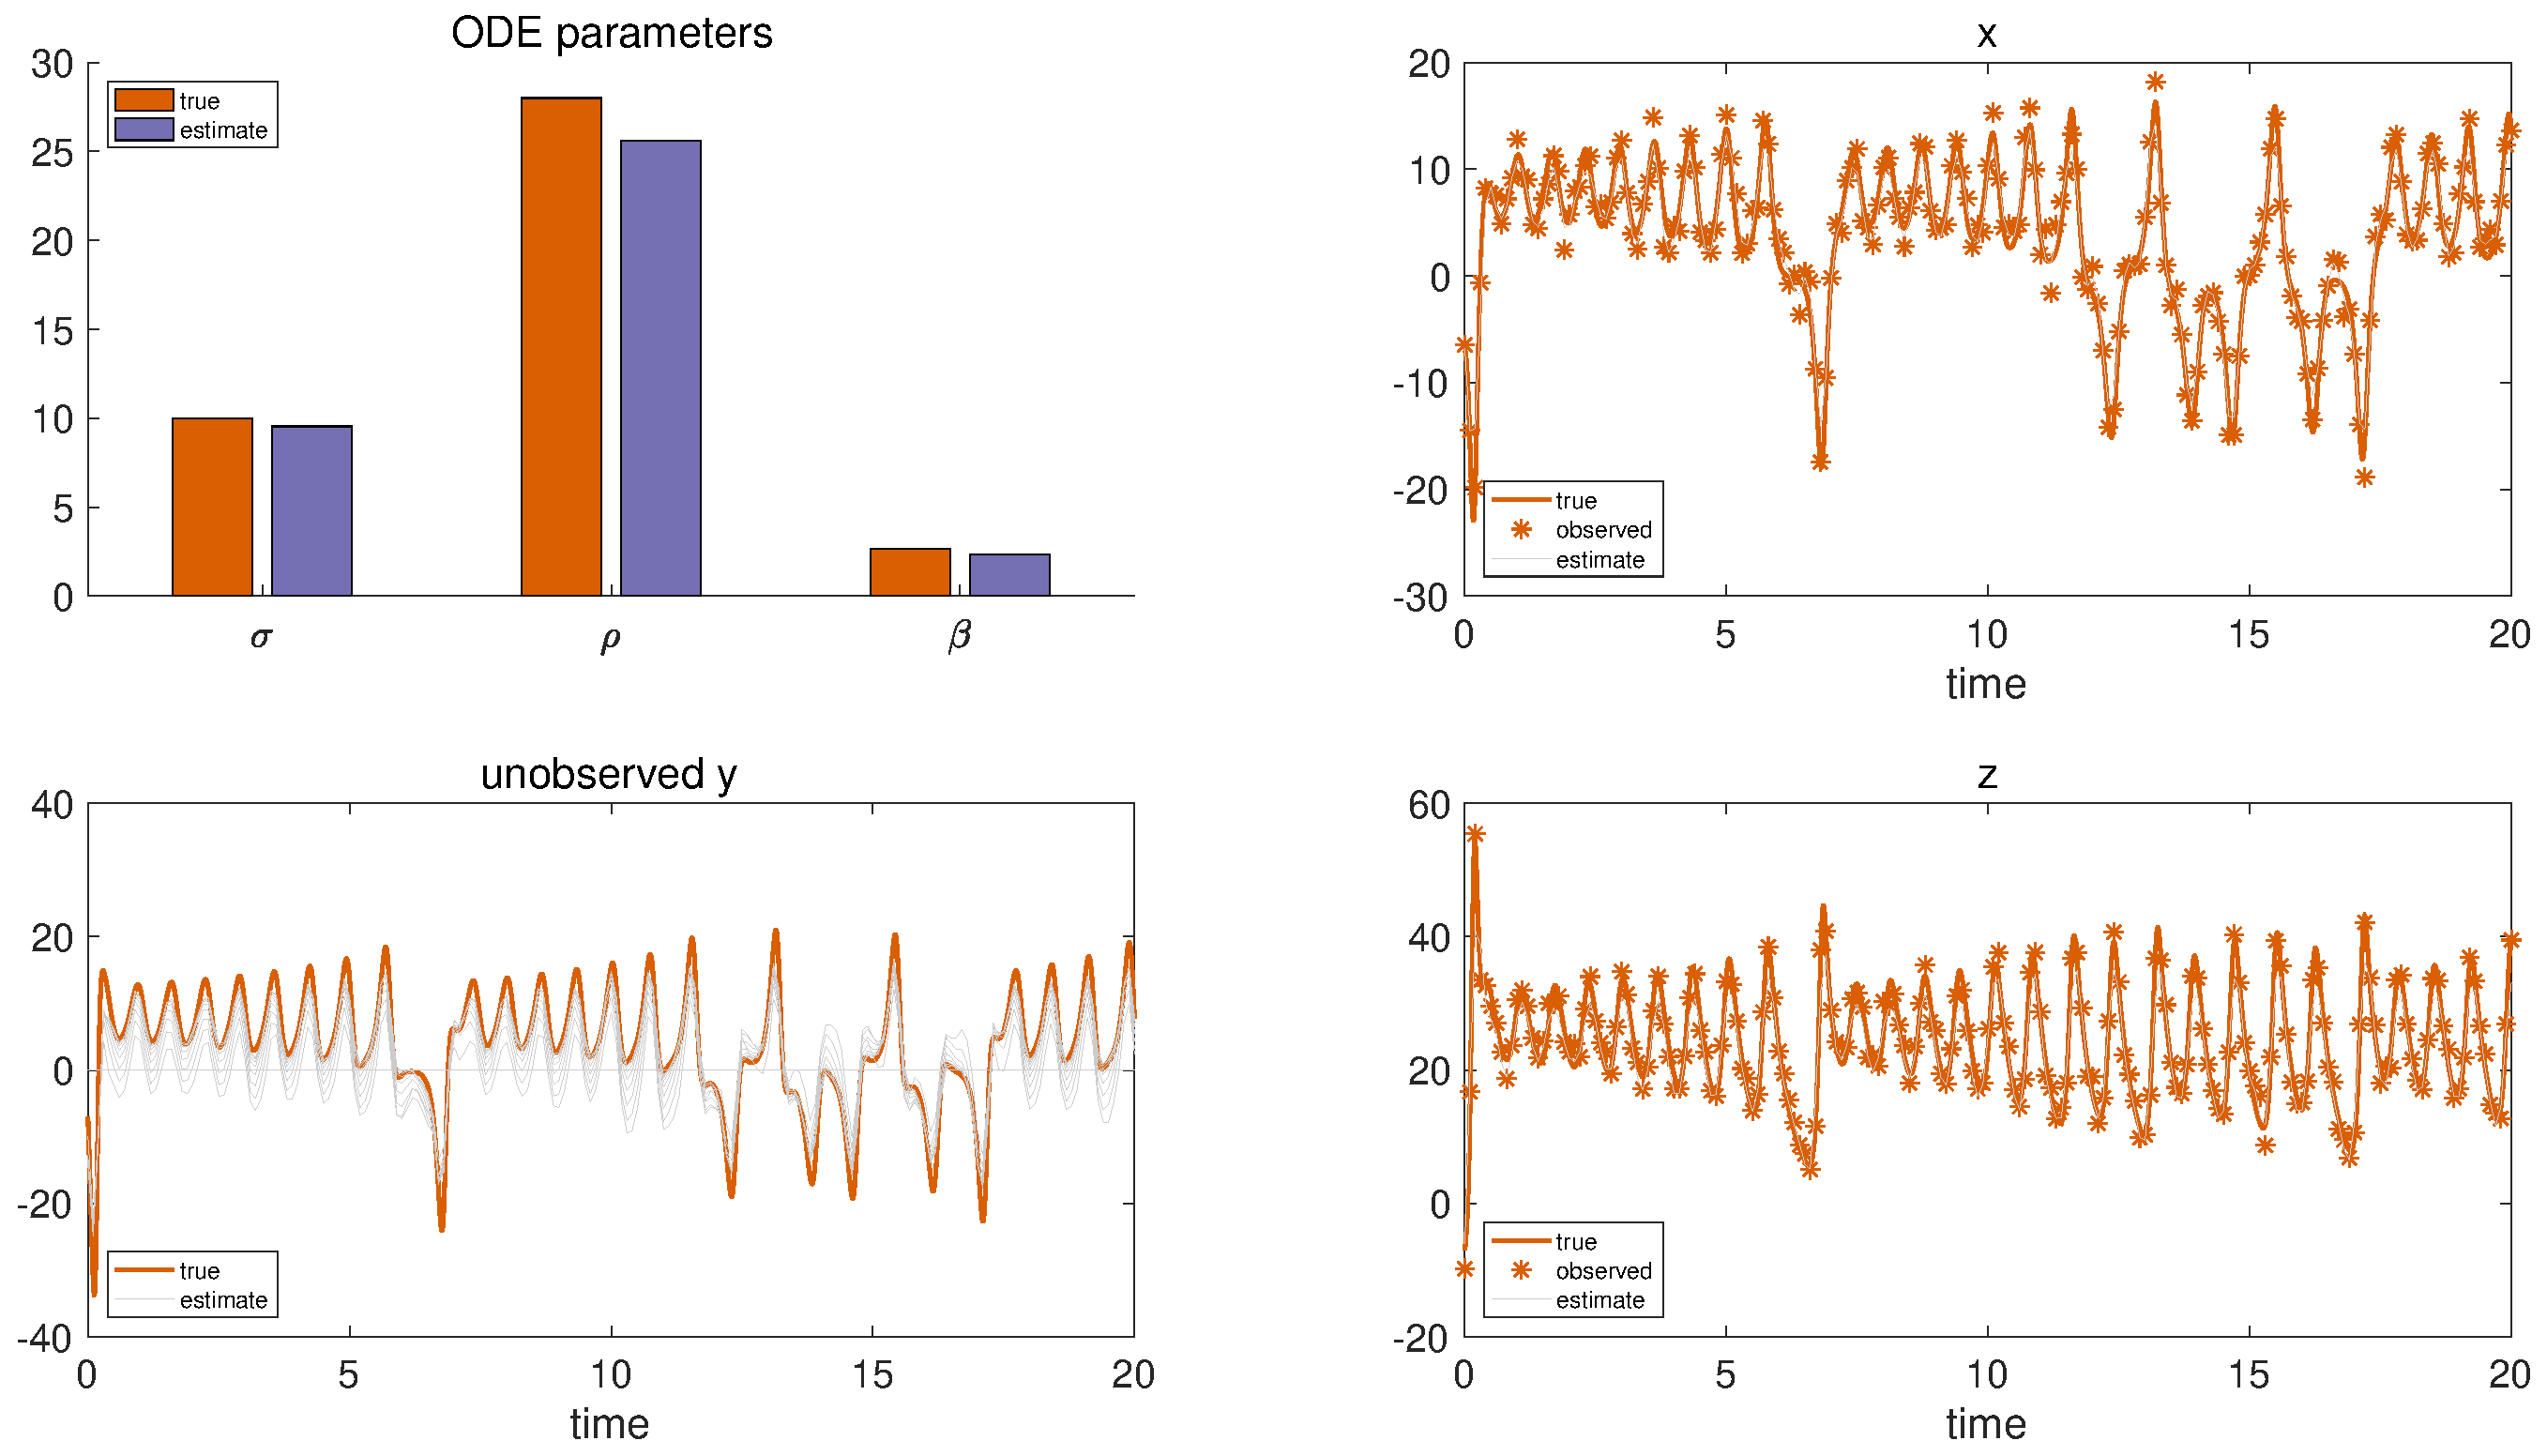
\includegraphics [width=5in]{Lorenz_attractor_4_13.eps}

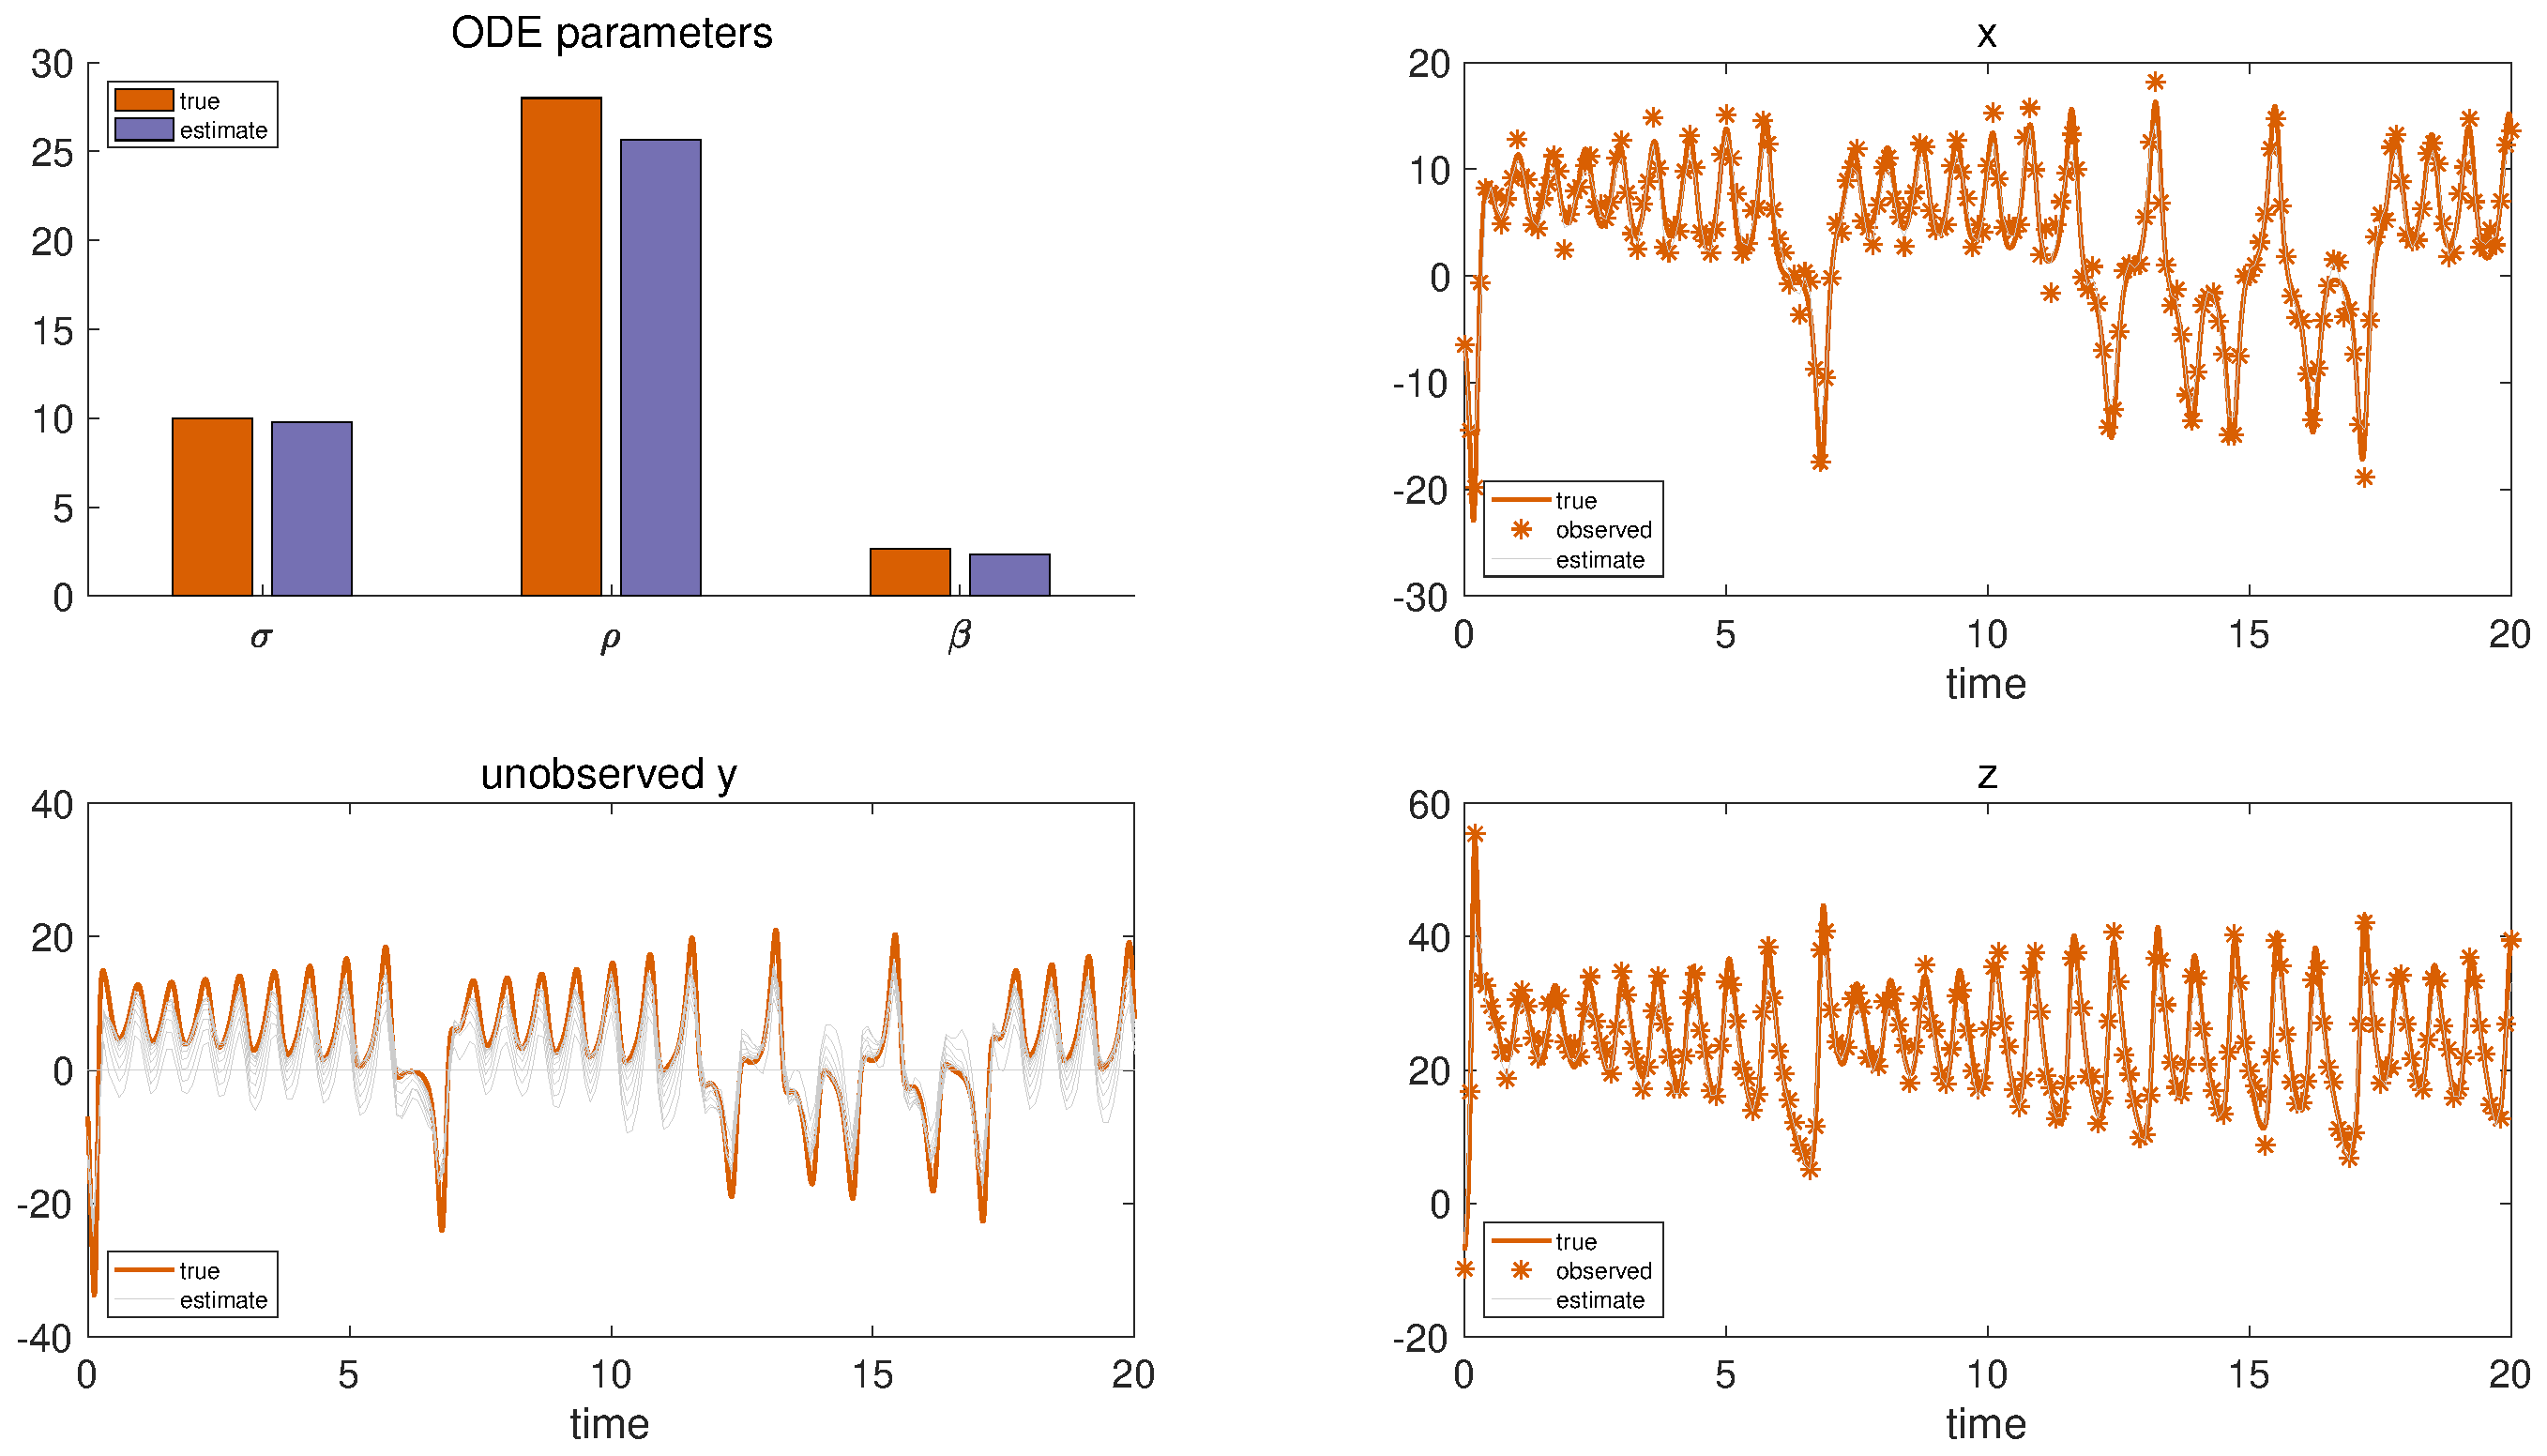
\includegraphics [width=5in]{Lorenz_attractor_4_14.eps}

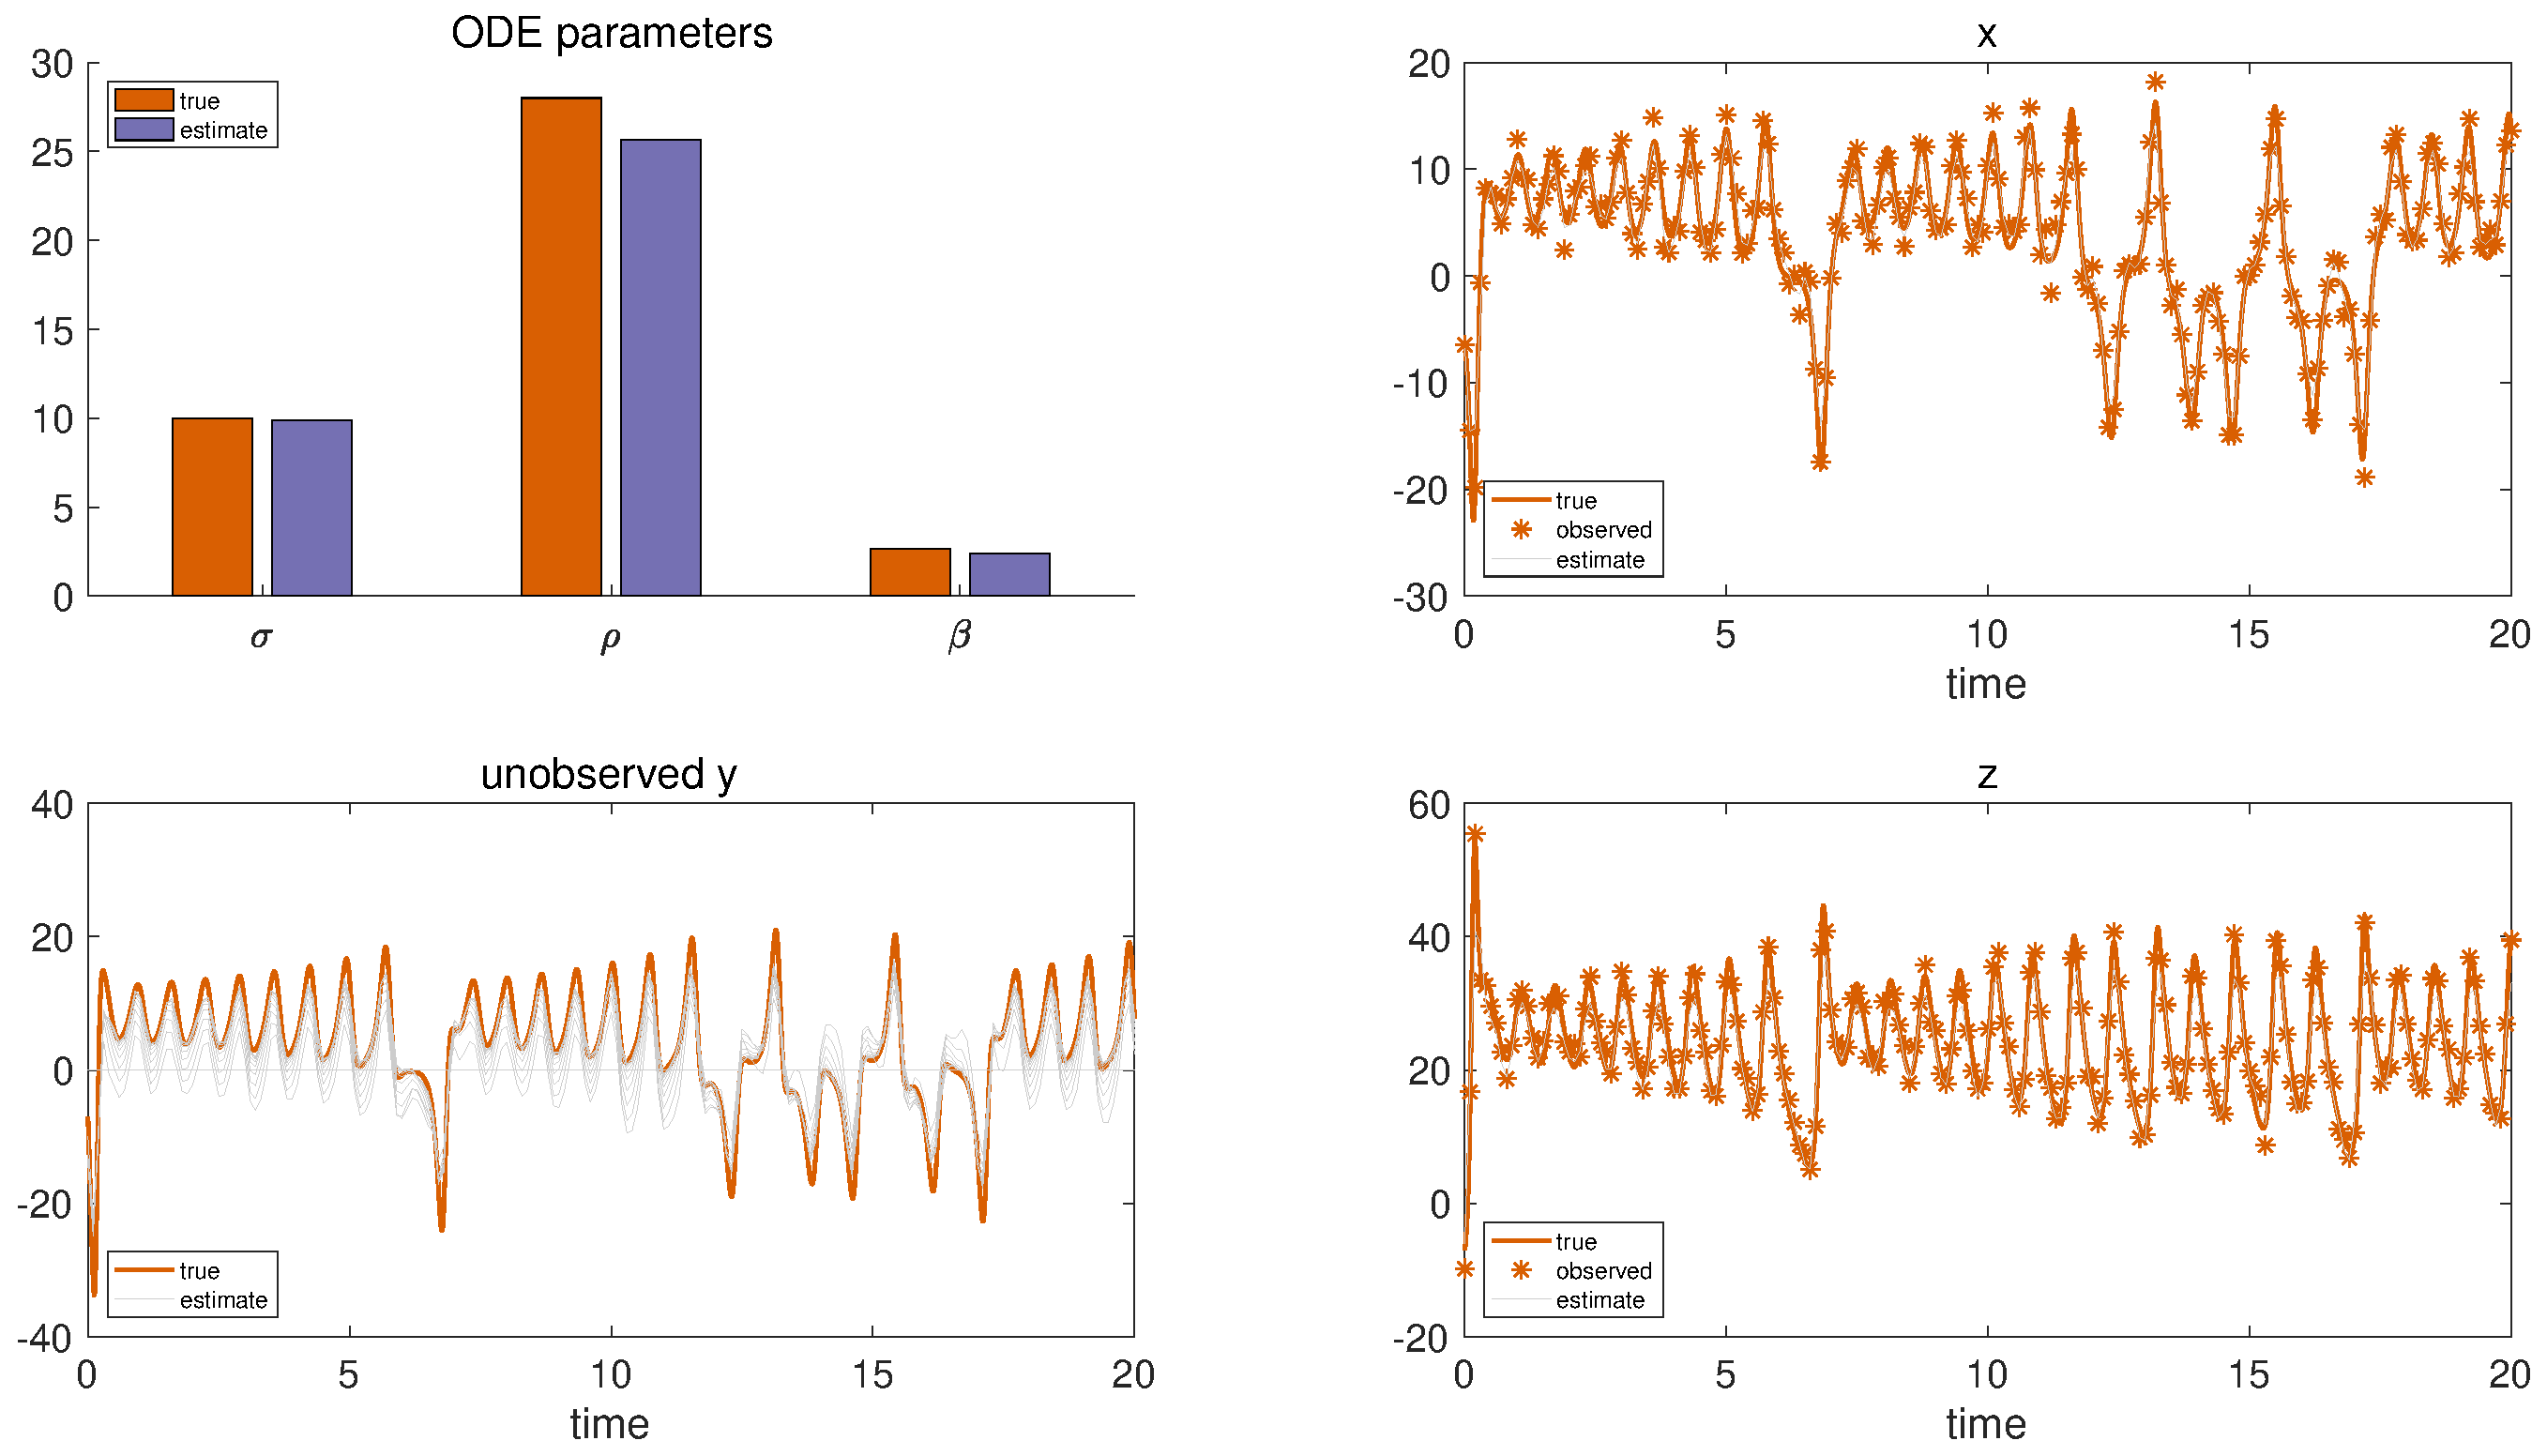
\includegraphics [width=5in]{Lorenz_attractor_4_15.eps}

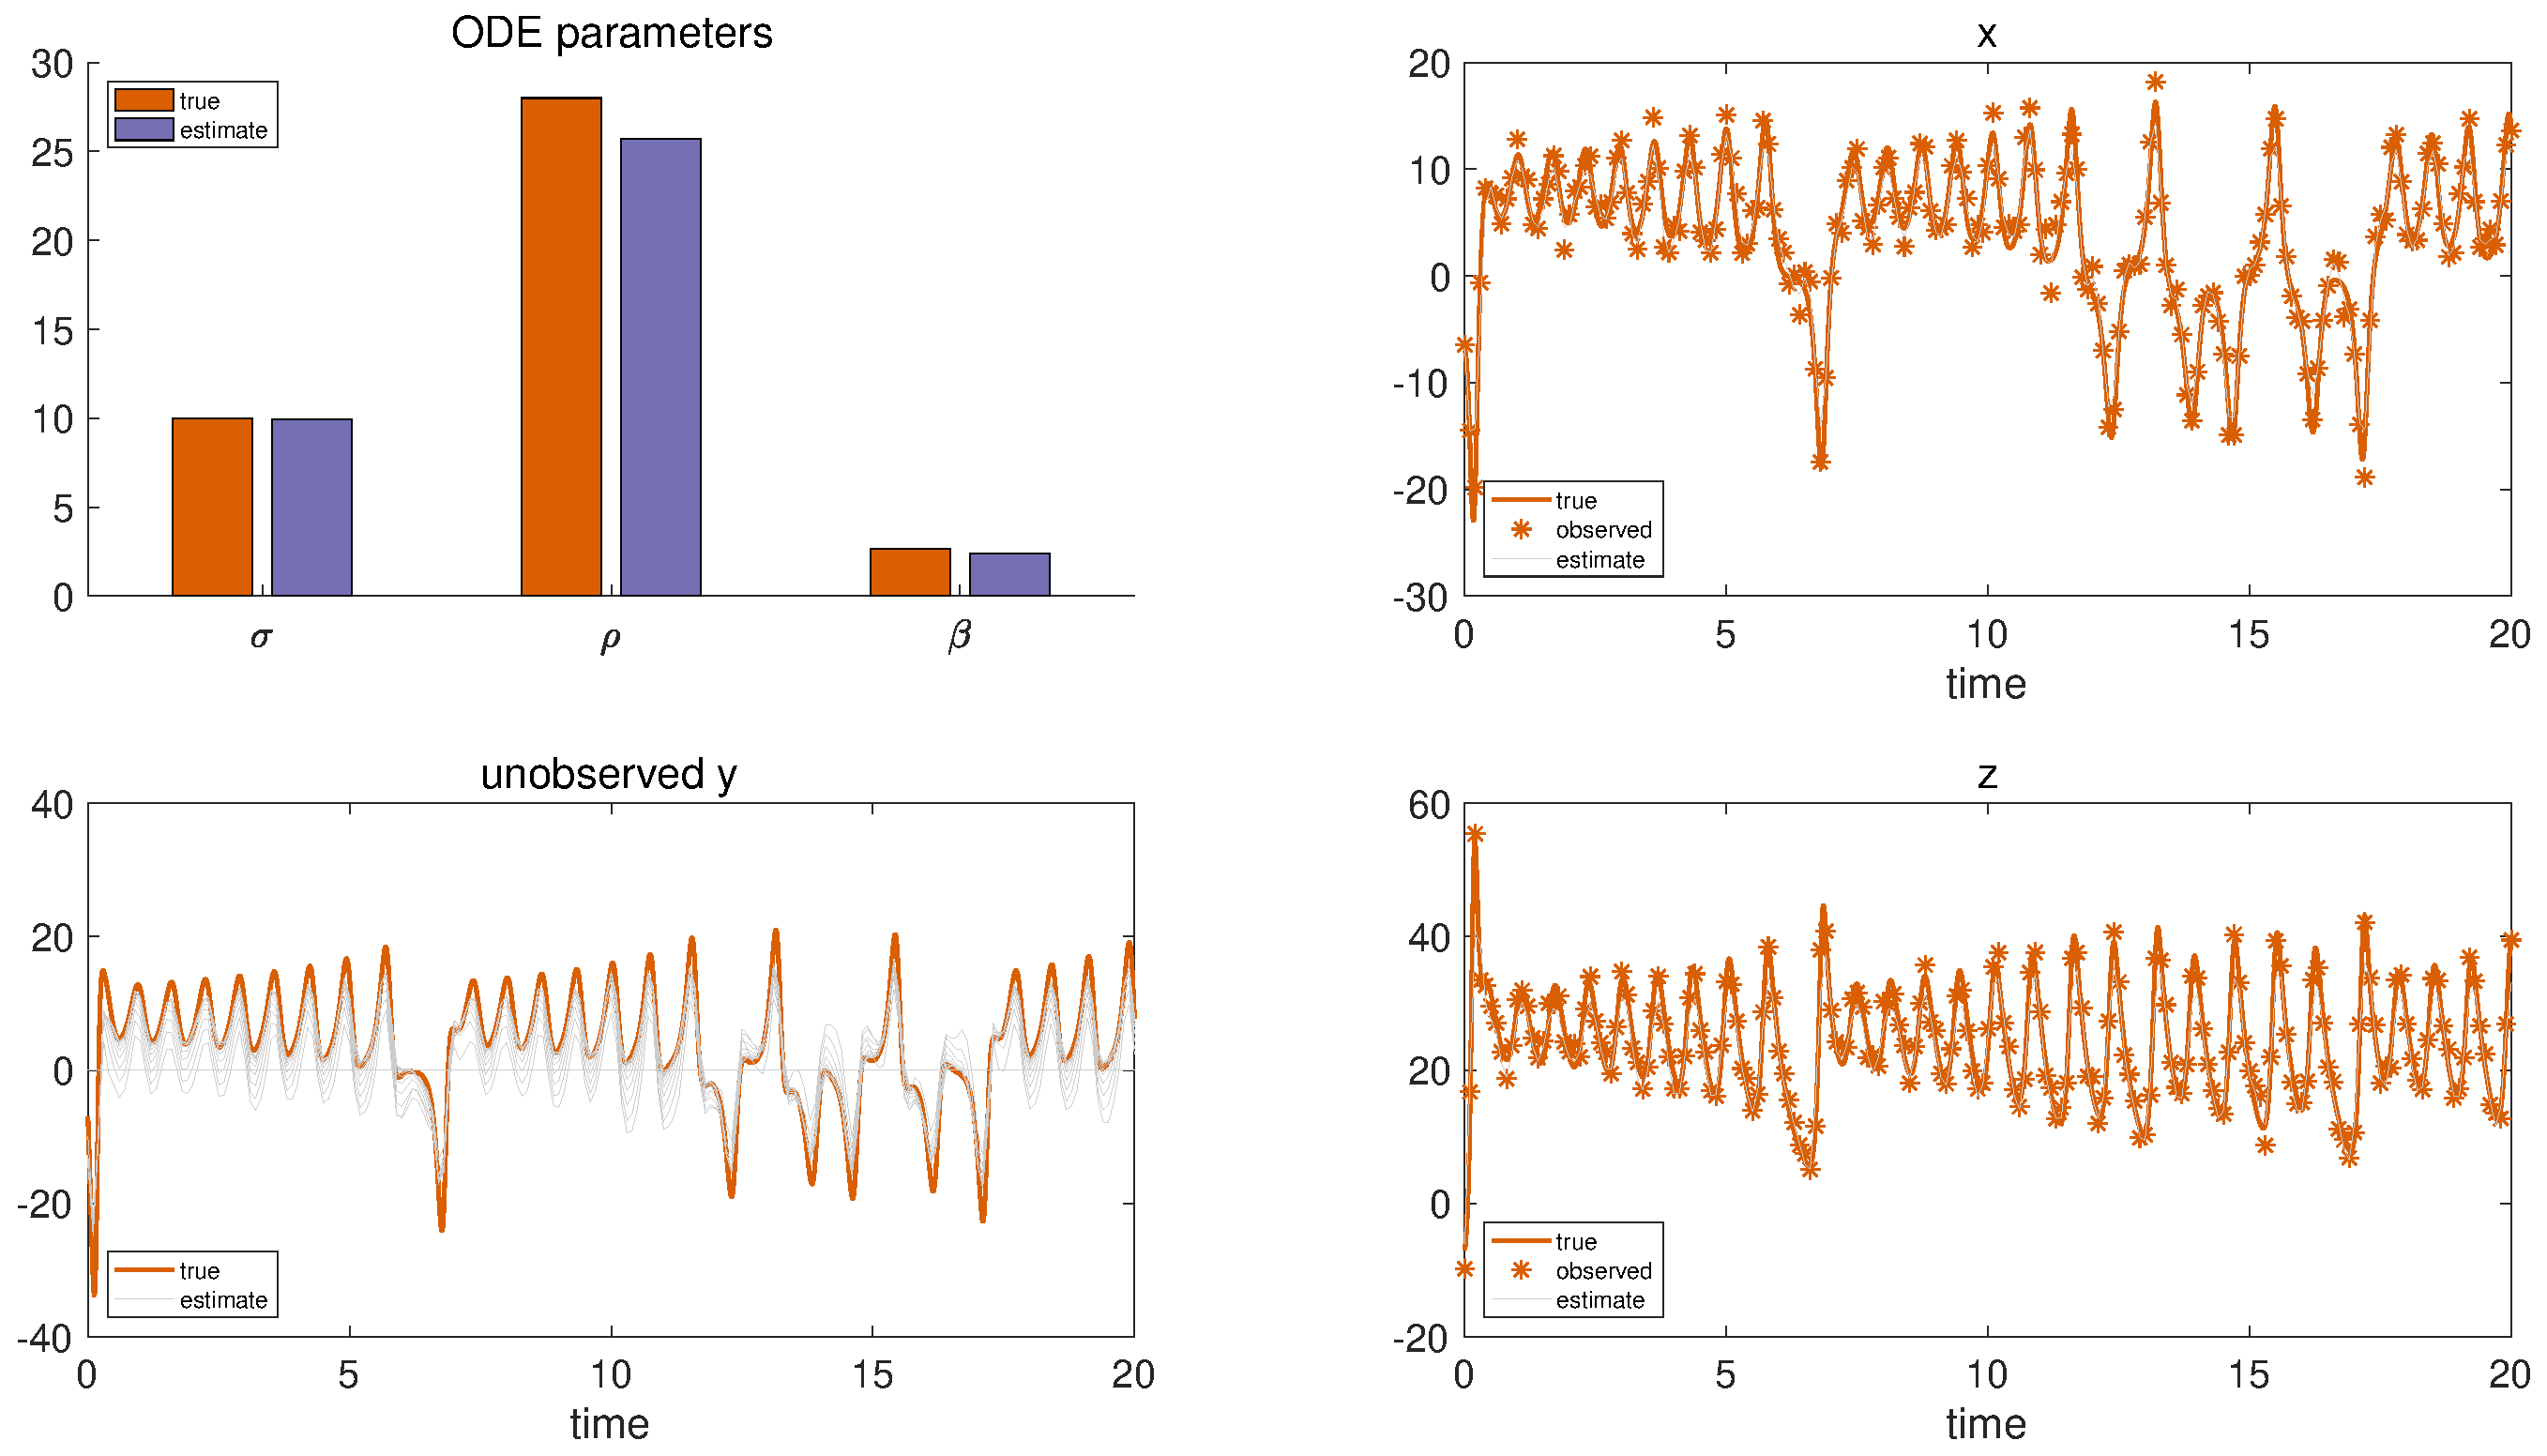
\includegraphics [width=5in]{Lorenz_attractor_4_16.eps}

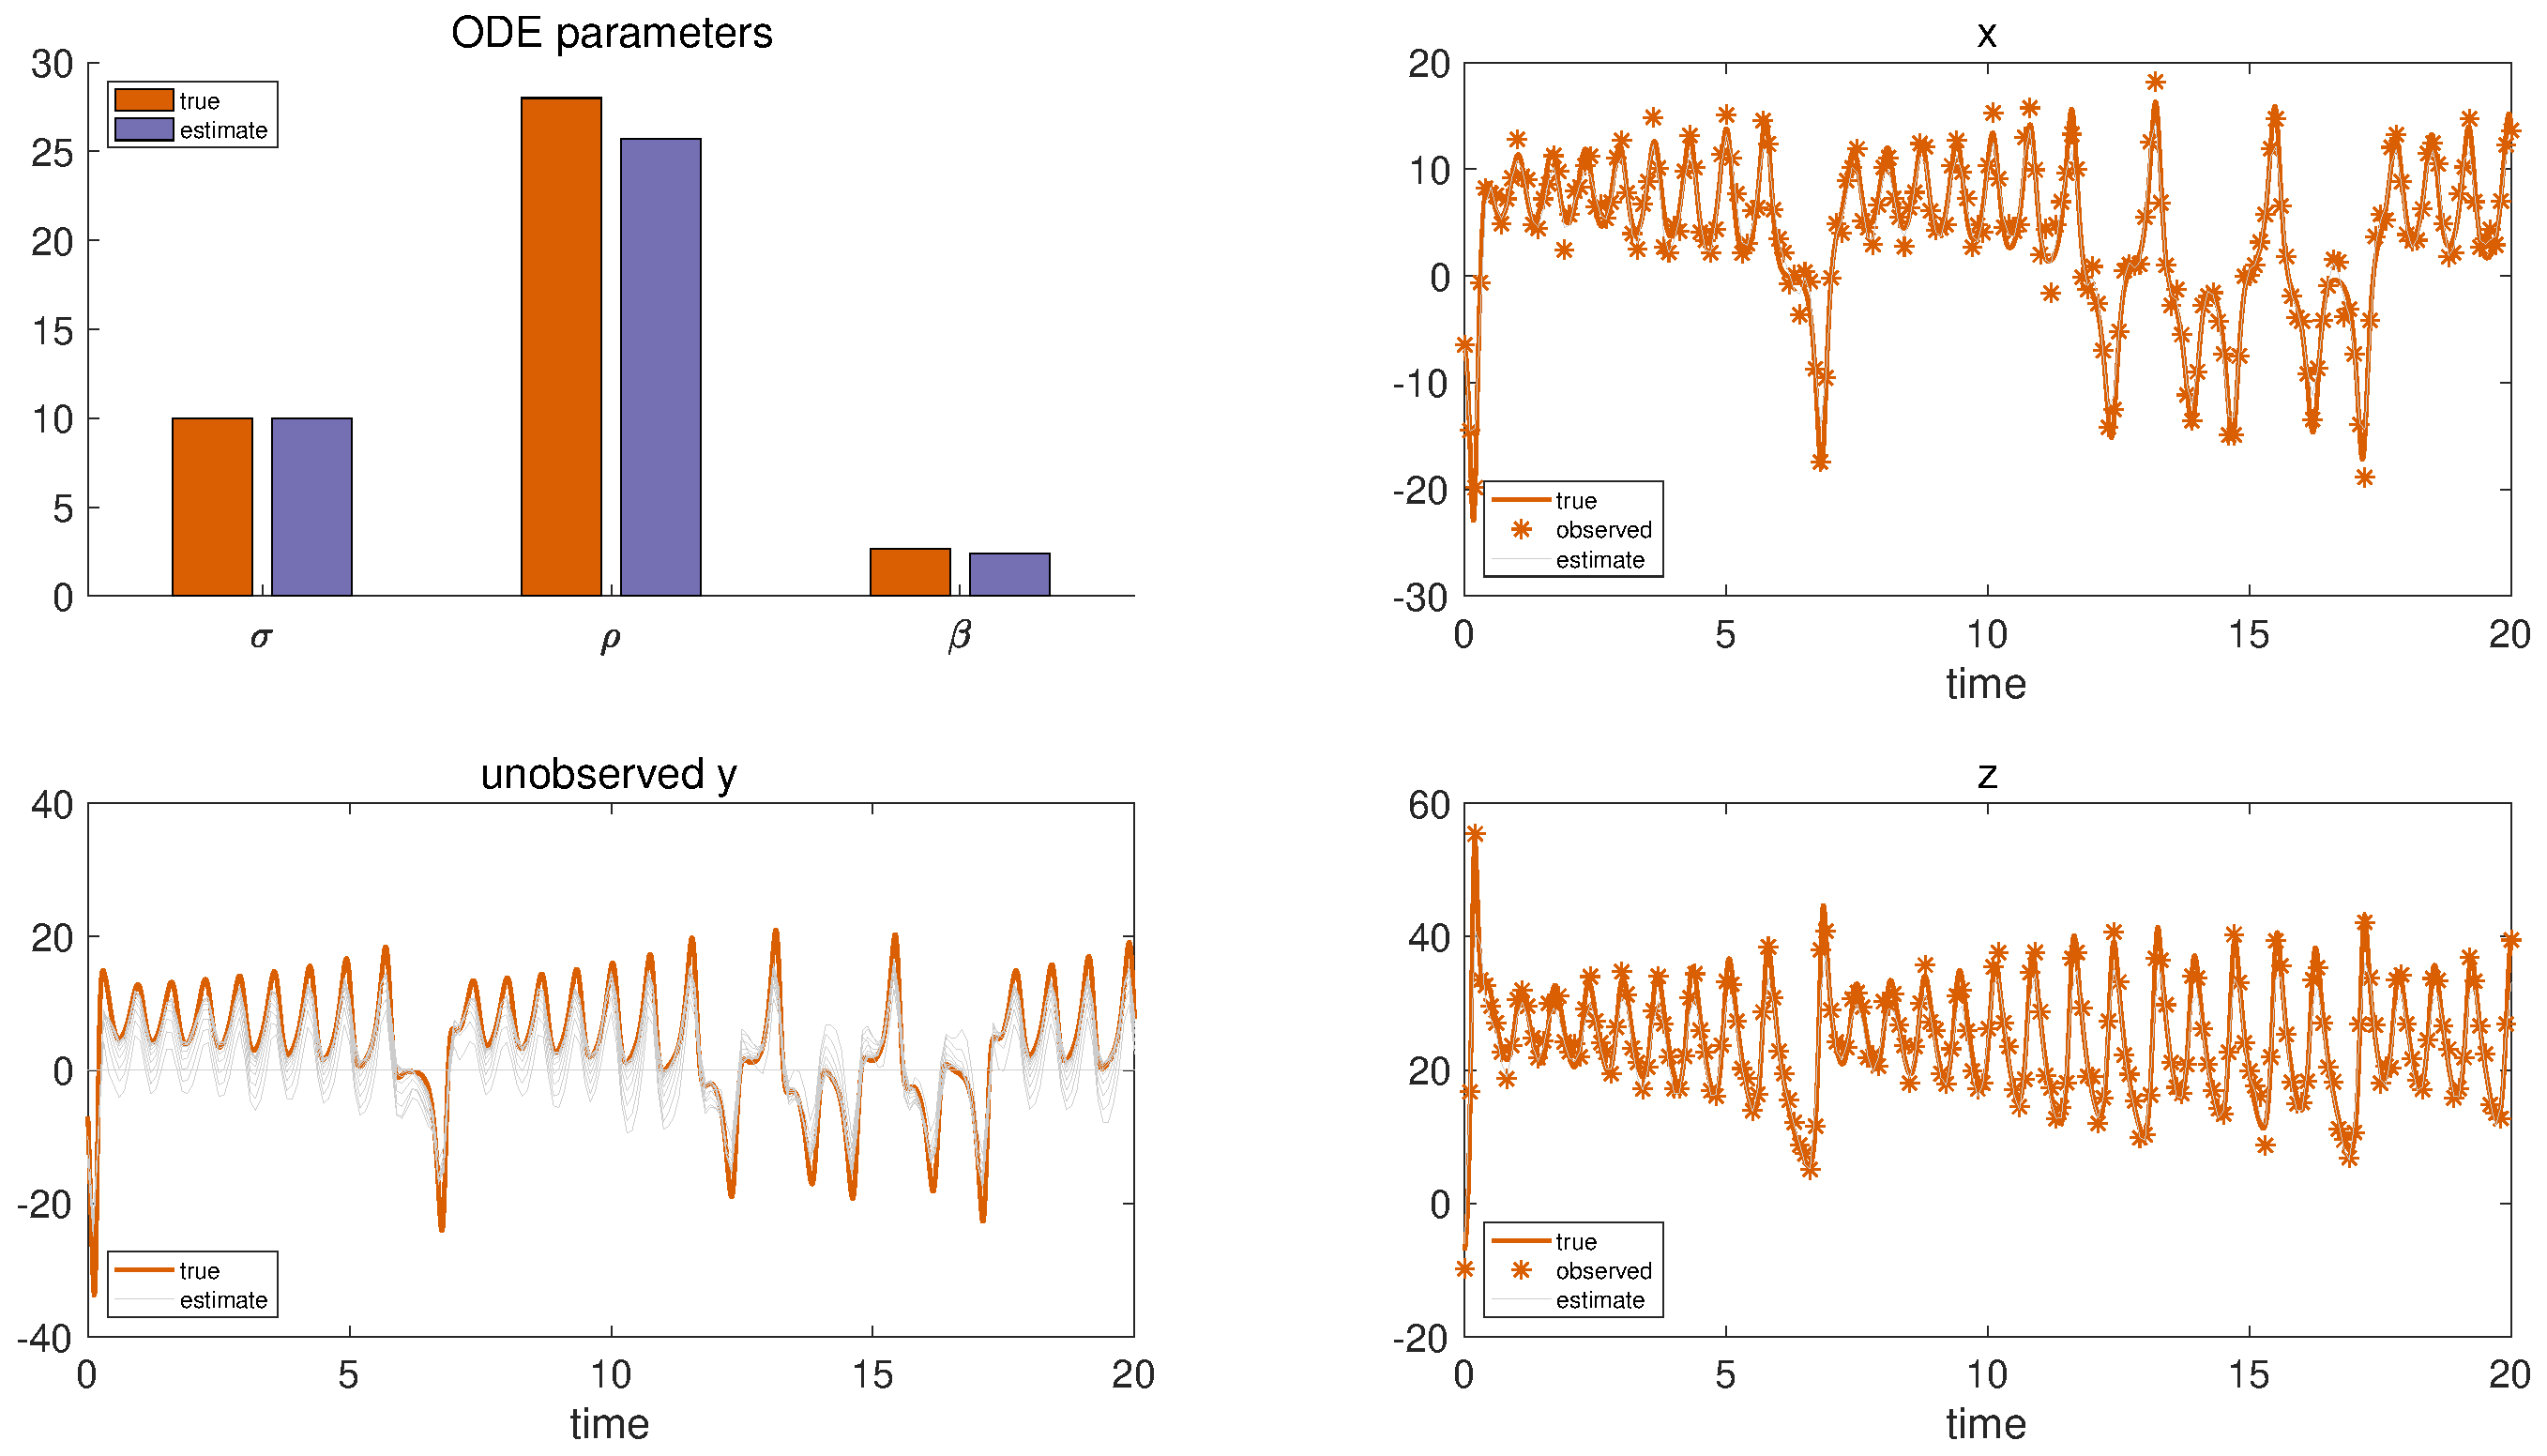
\includegraphics [width=5in]{Lorenz_attractor_4_17.eps}

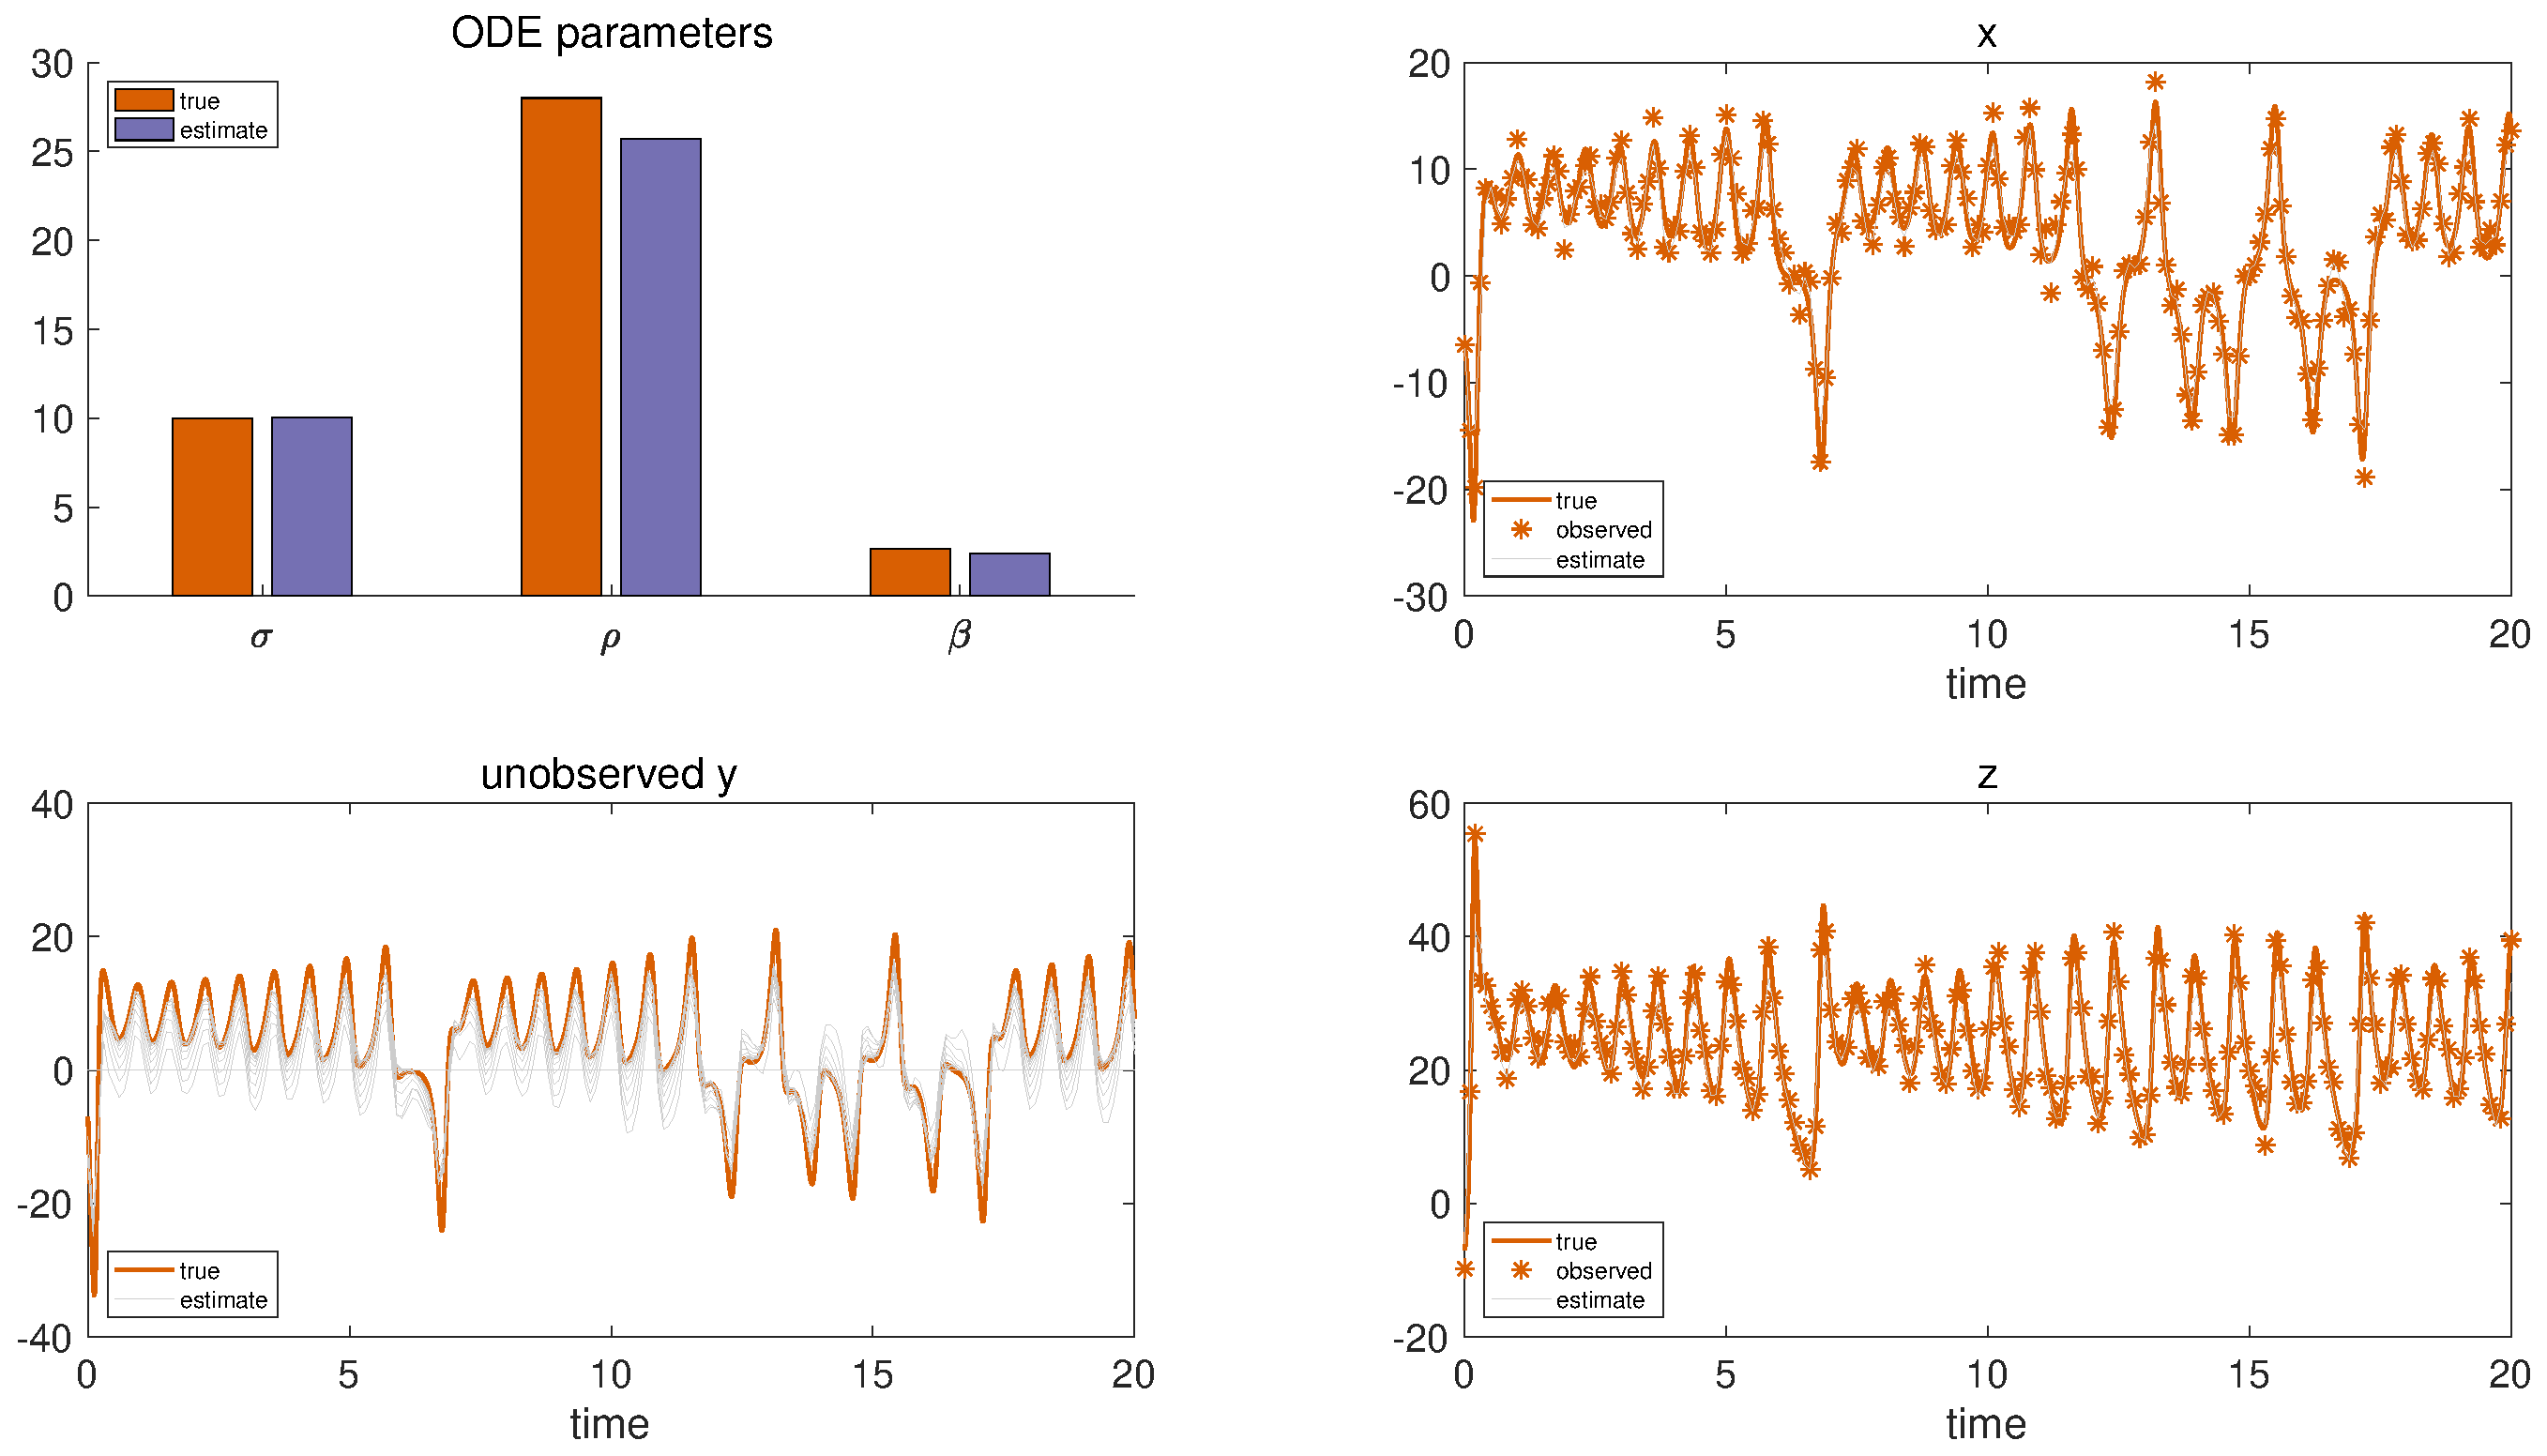
\includegraphics [width=5in]{Lorenz_attractor_4_18.eps}

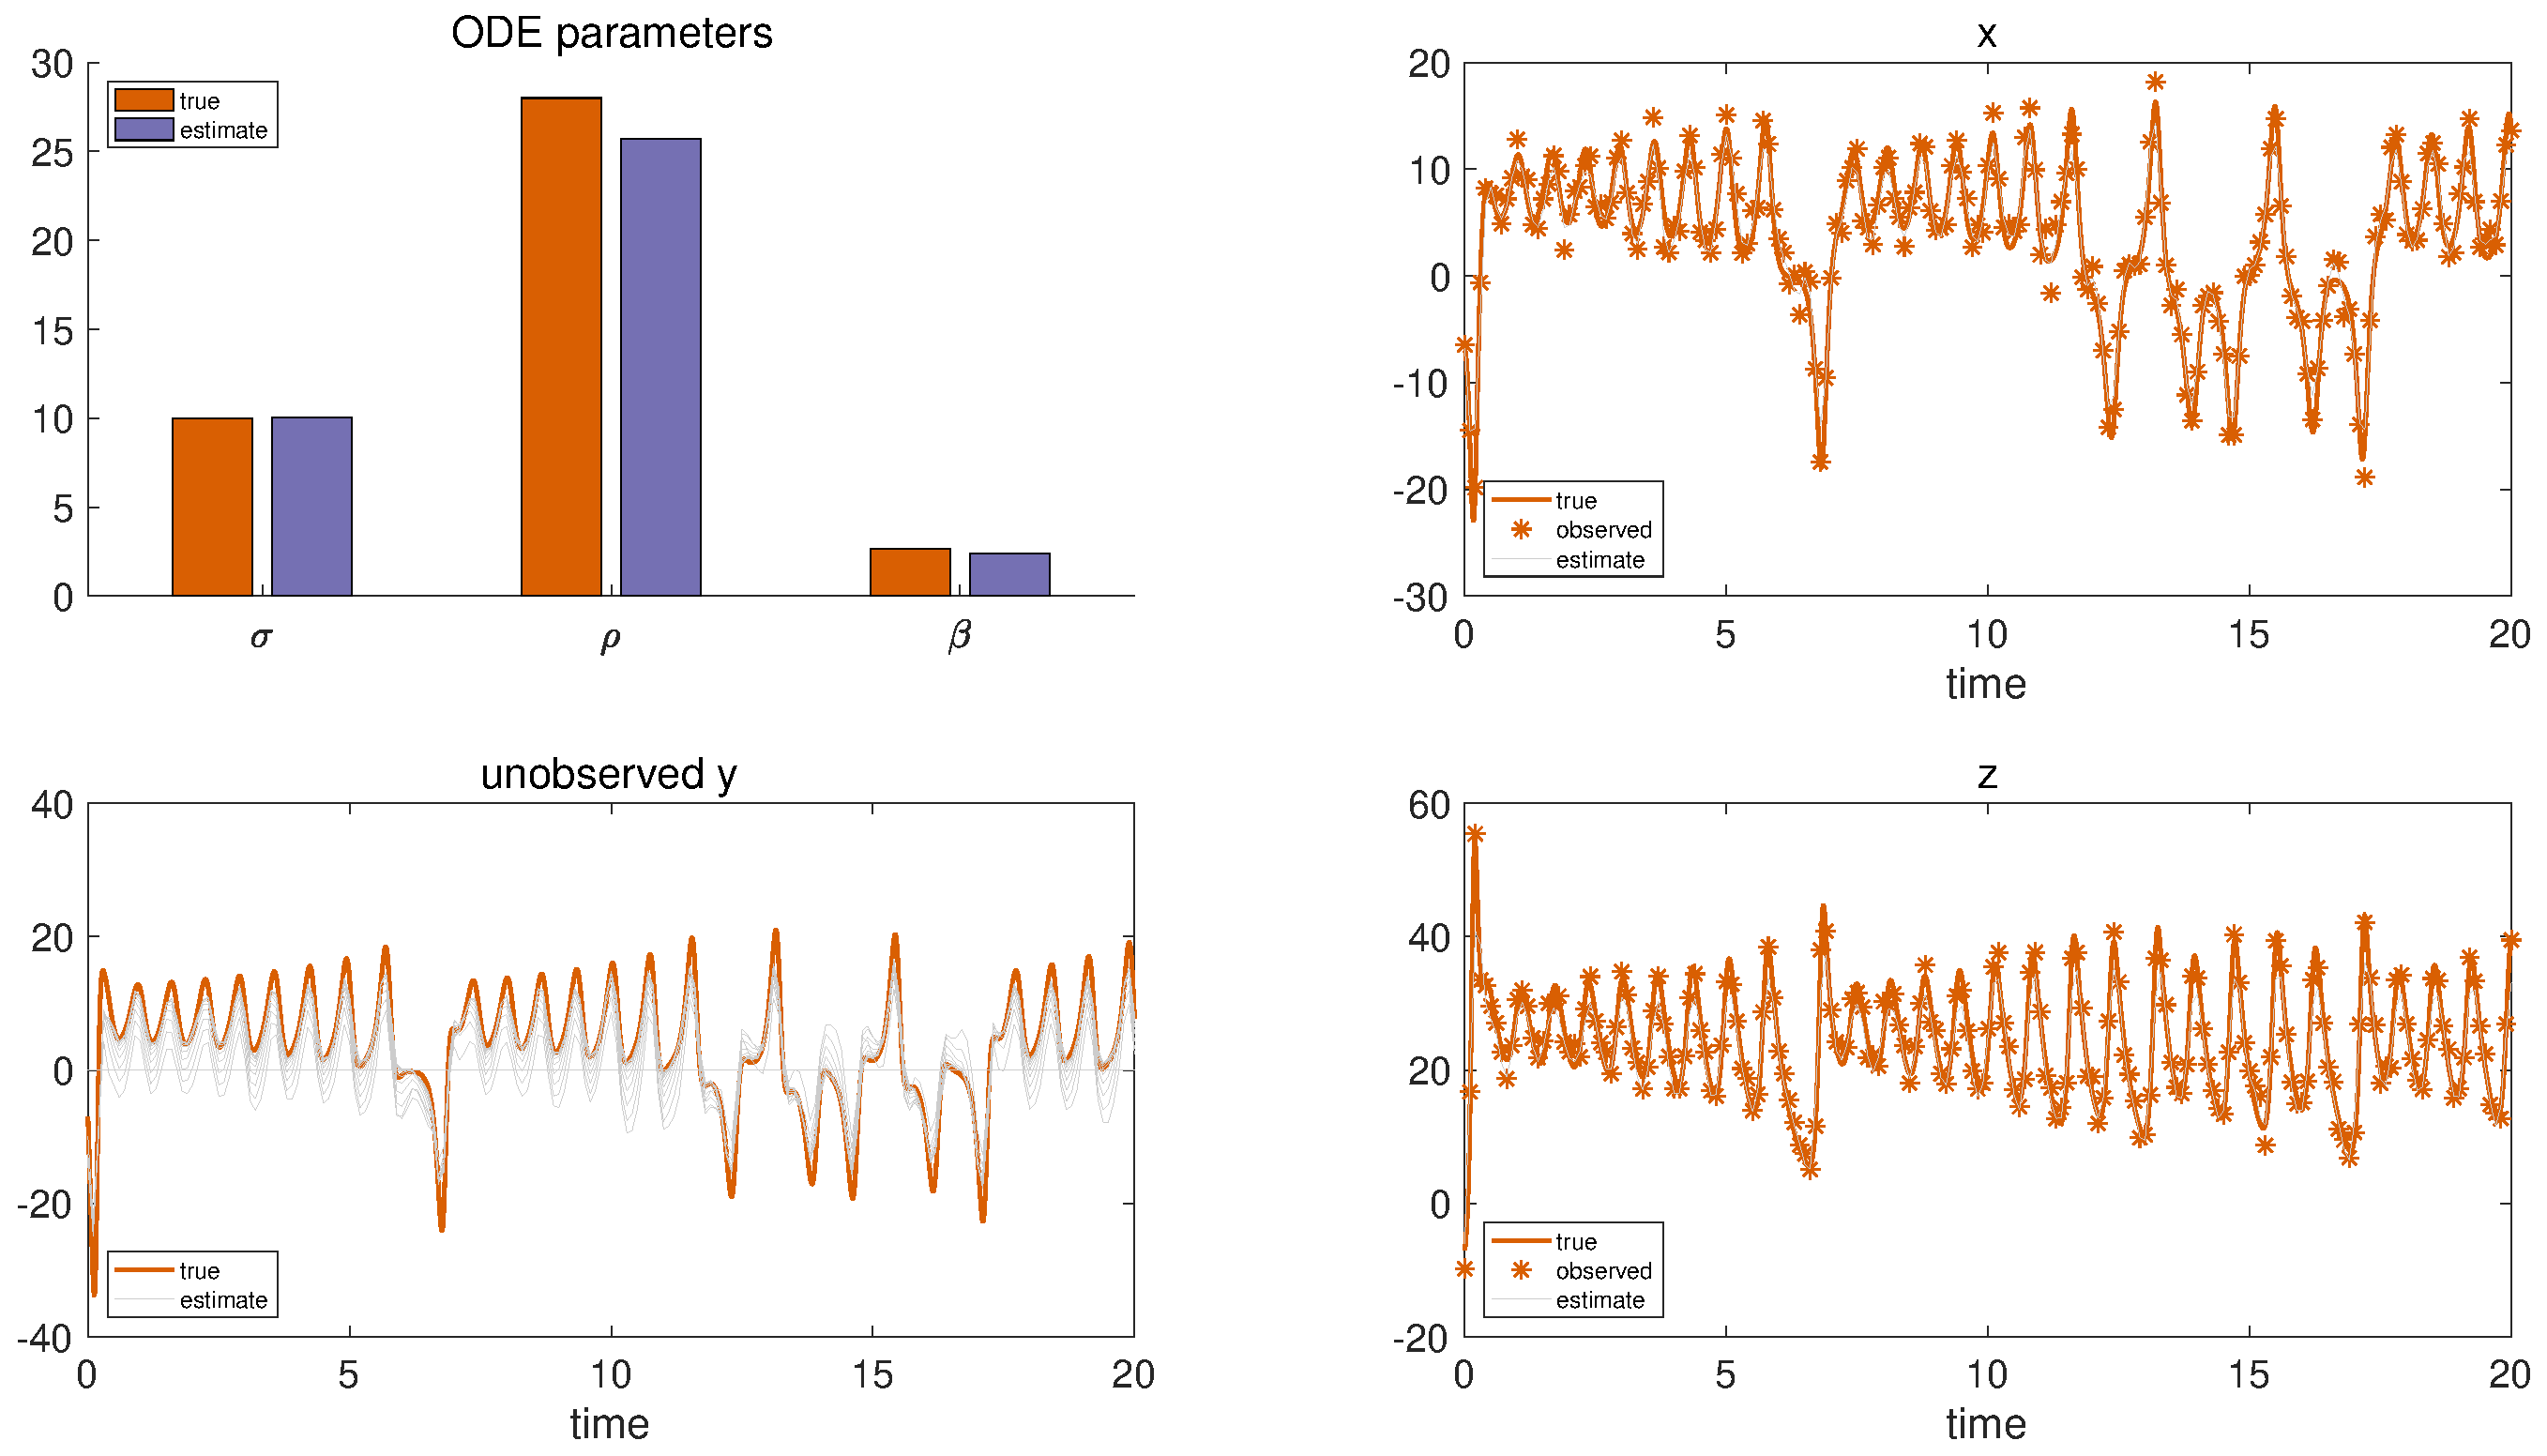
\includegraphics [width=5in]{Lorenz_attractor_4_19.eps}

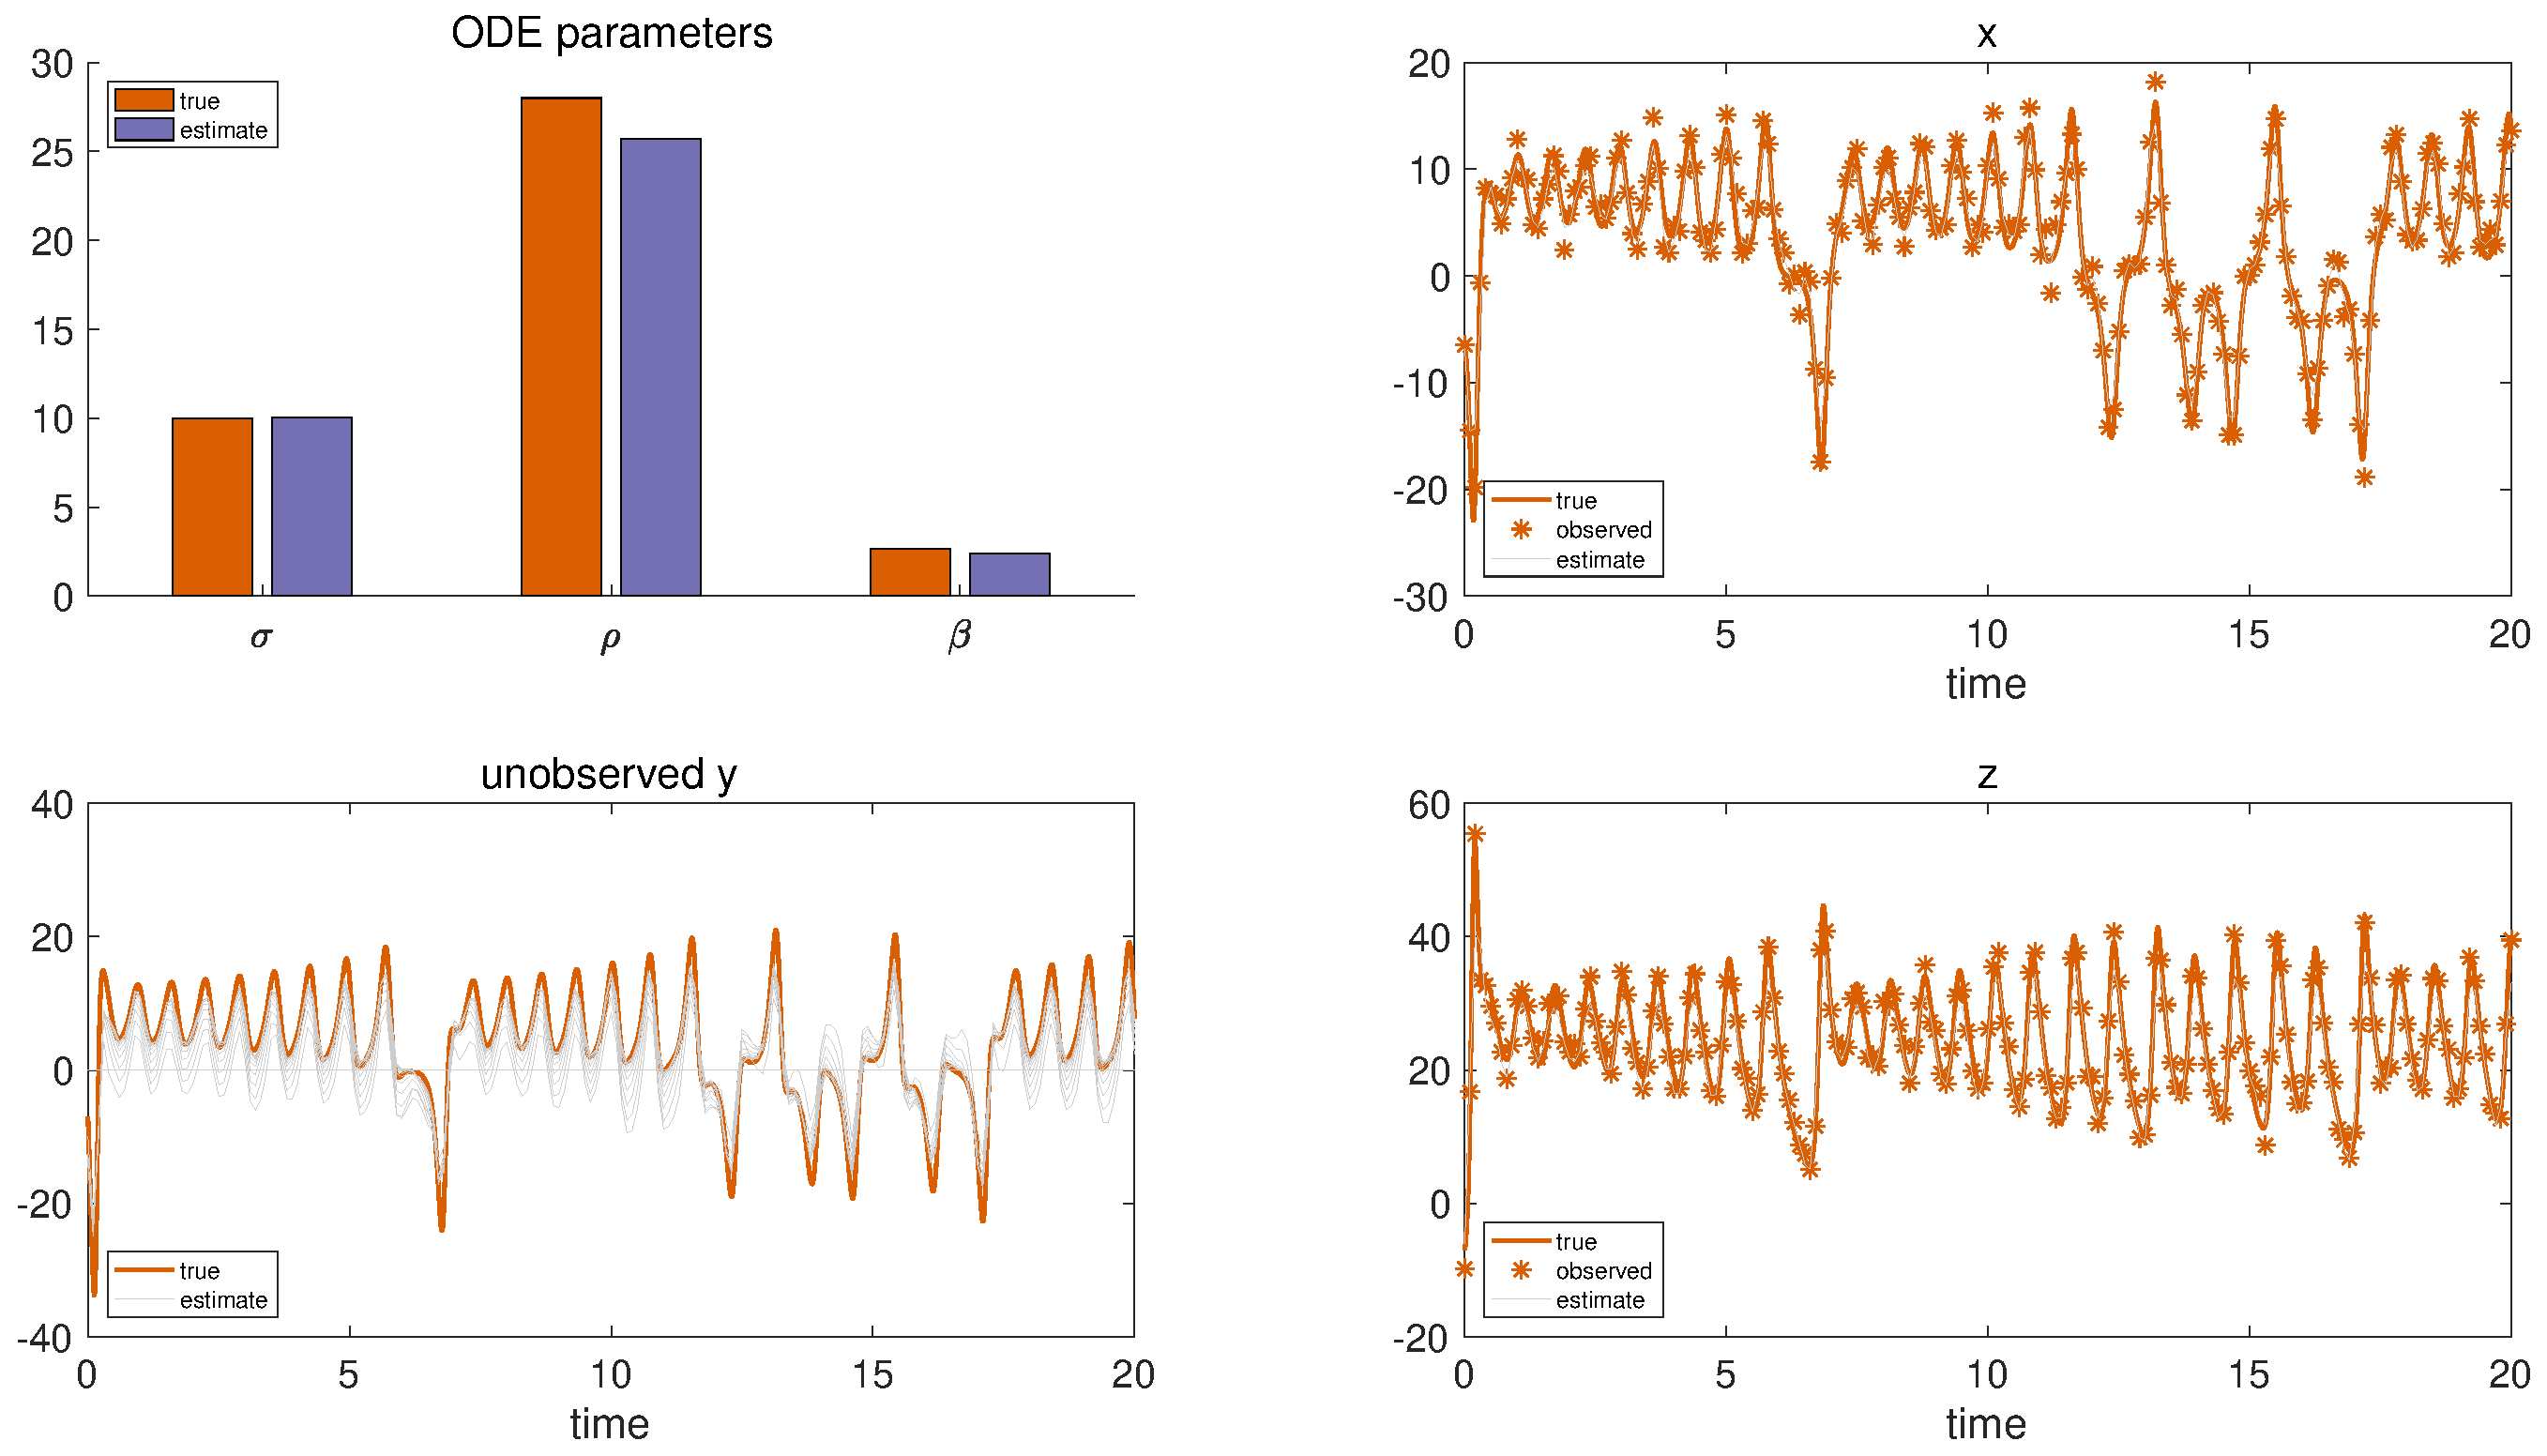
\includegraphics [width=5in]{Lorenz_attractor_4_20.eps}

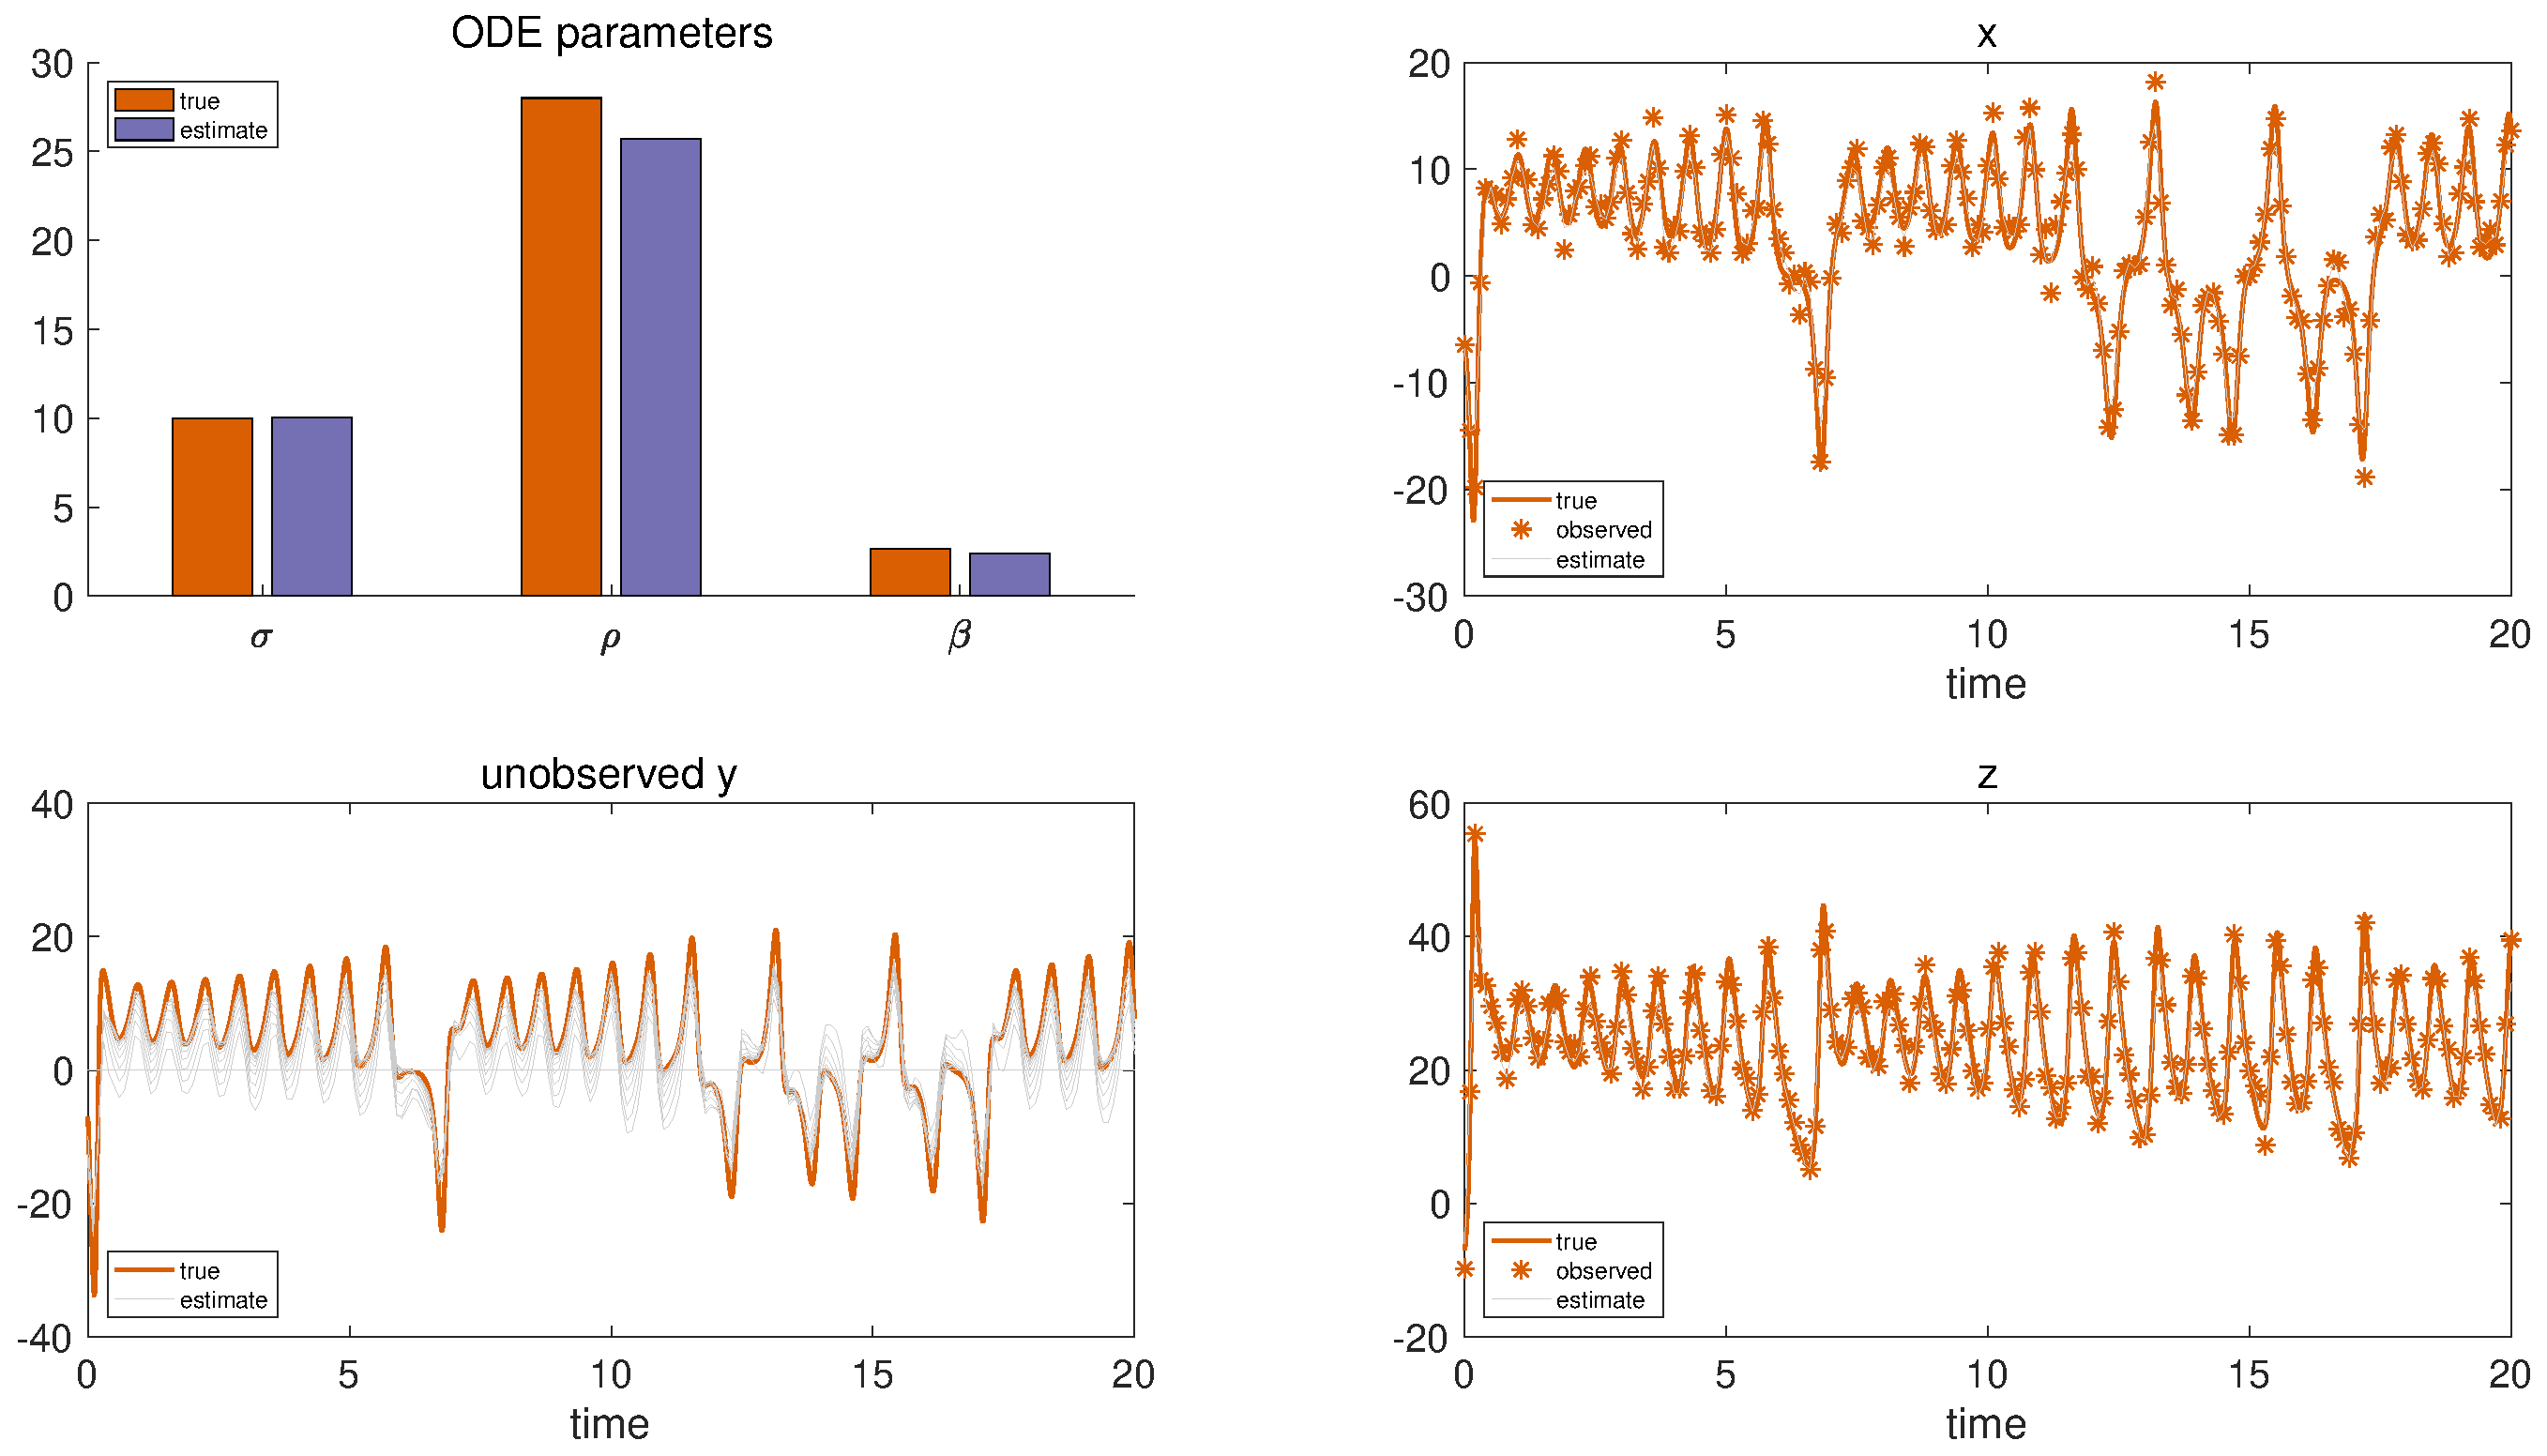
\includegraphics [width=5in]{Lorenz_attractor_4_21.eps}

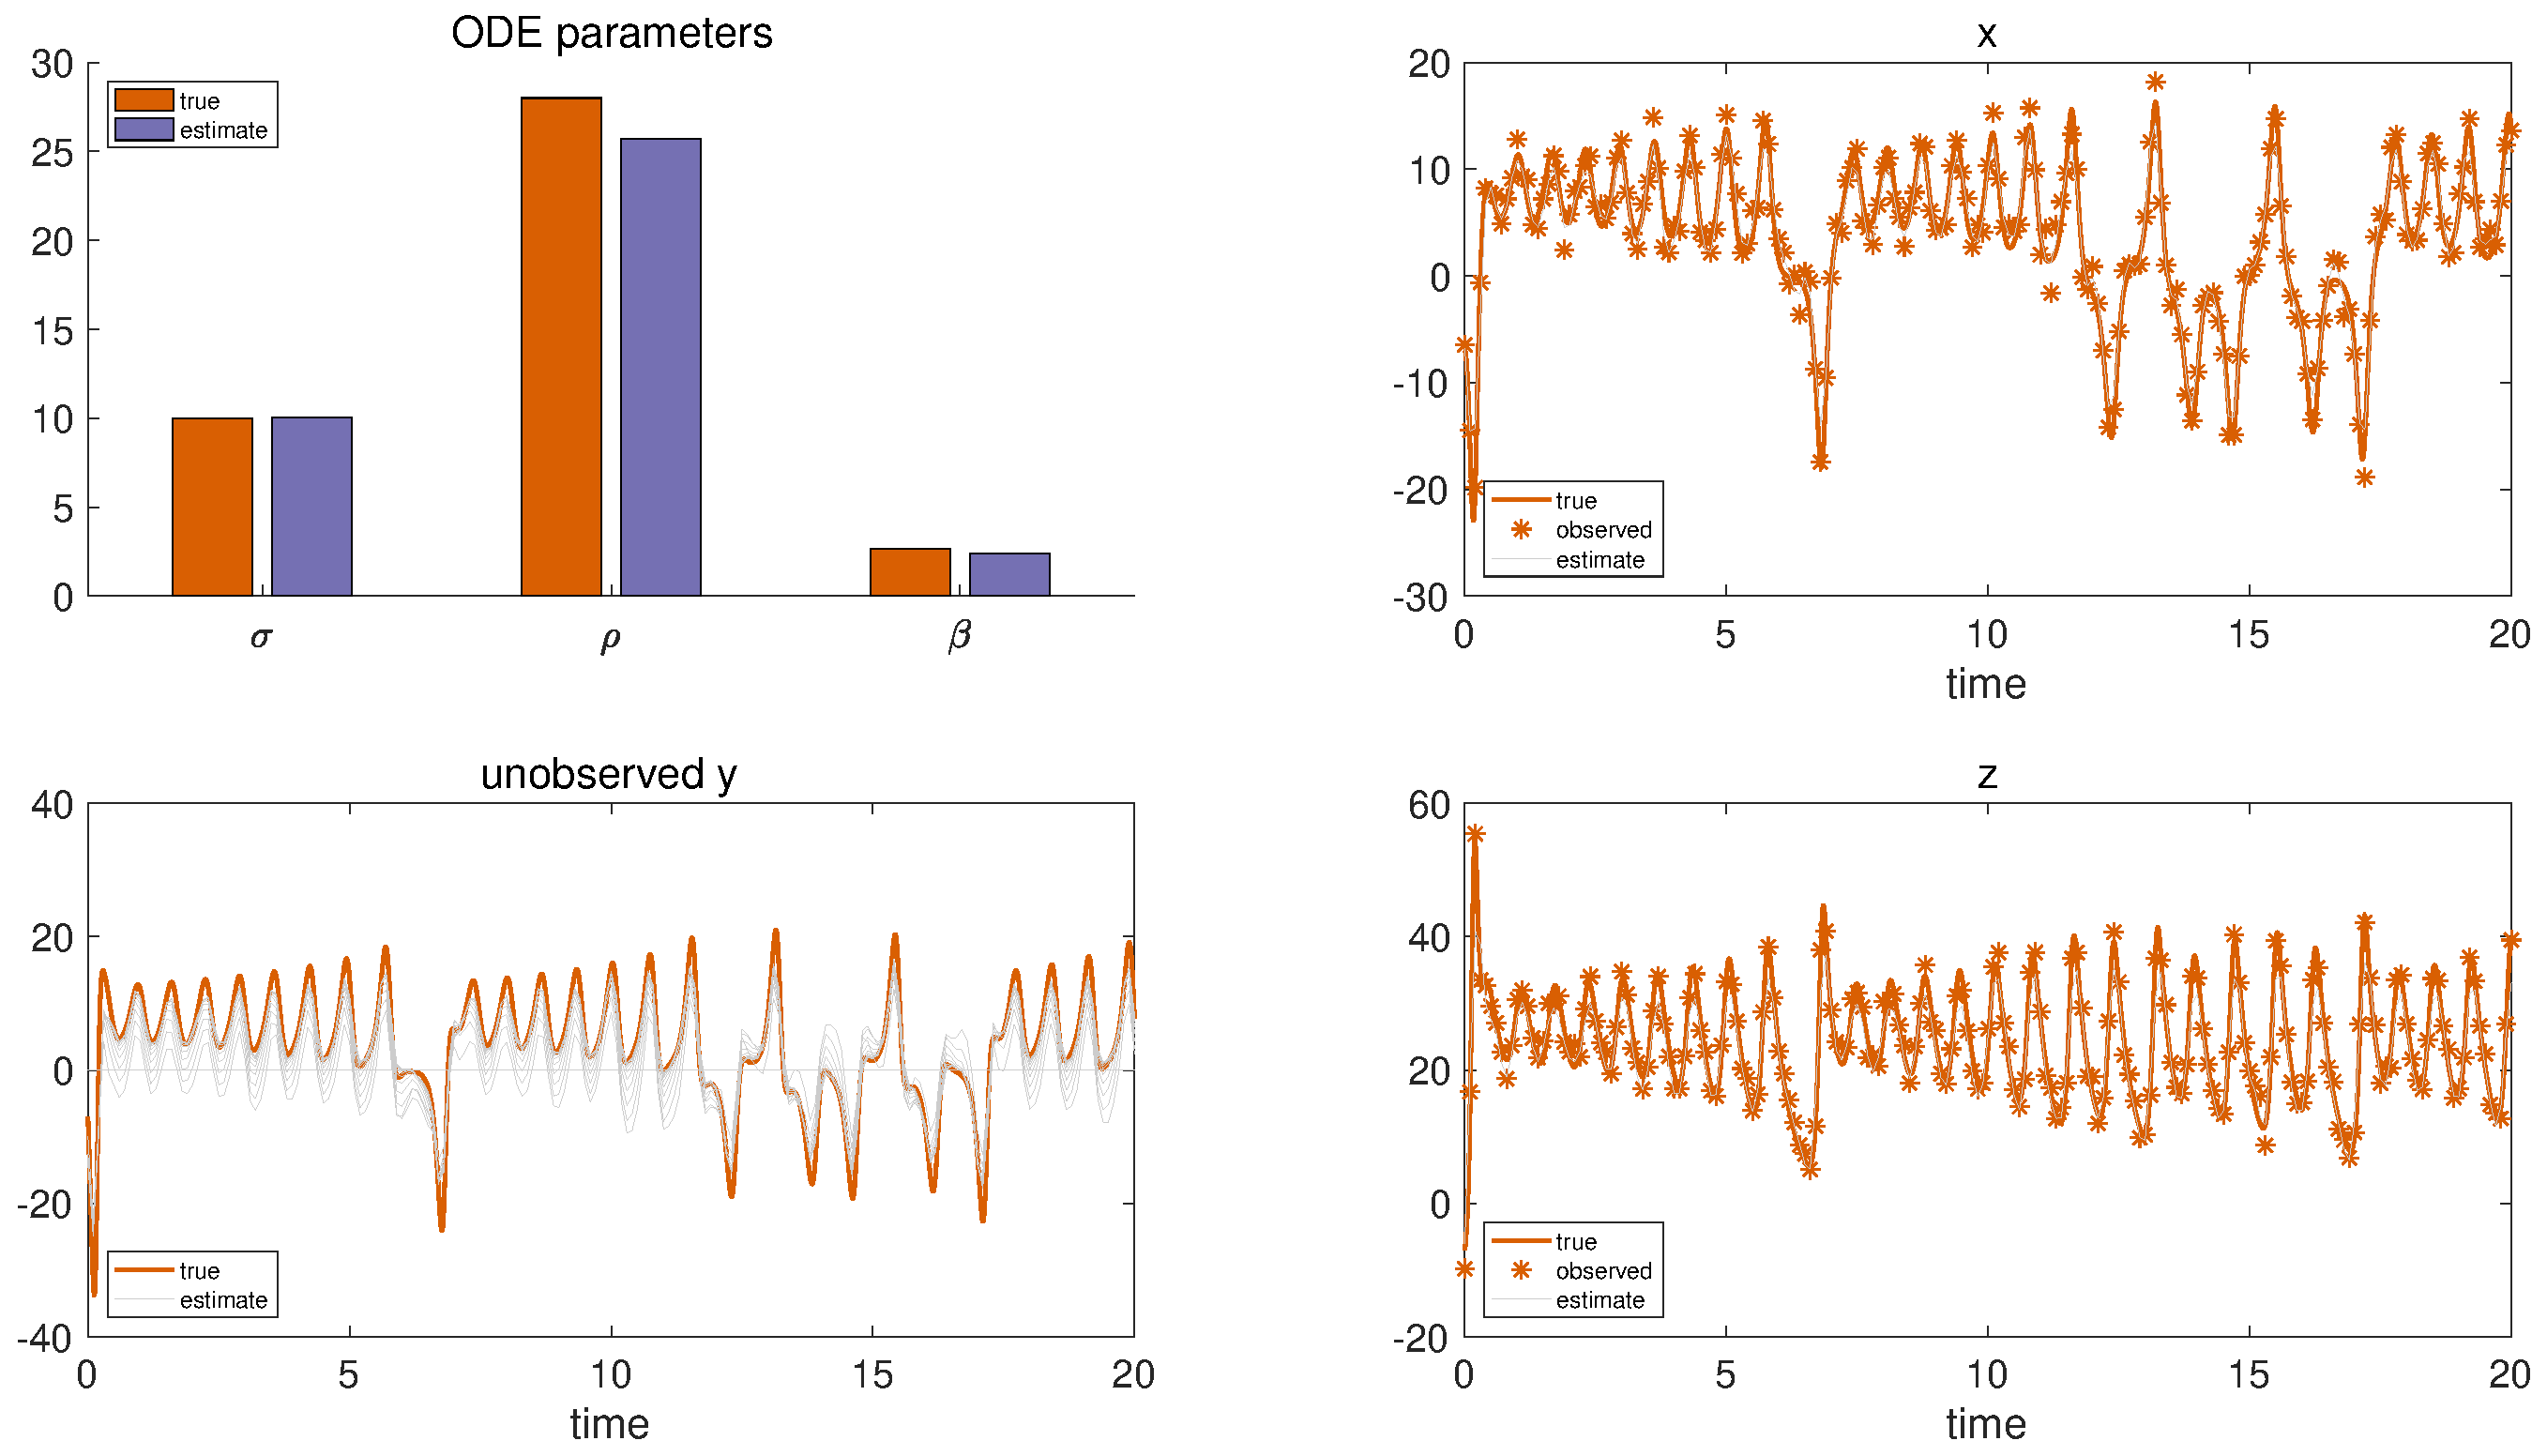
\includegraphics [width=5in]{Lorenz_attractor_4_22.eps}

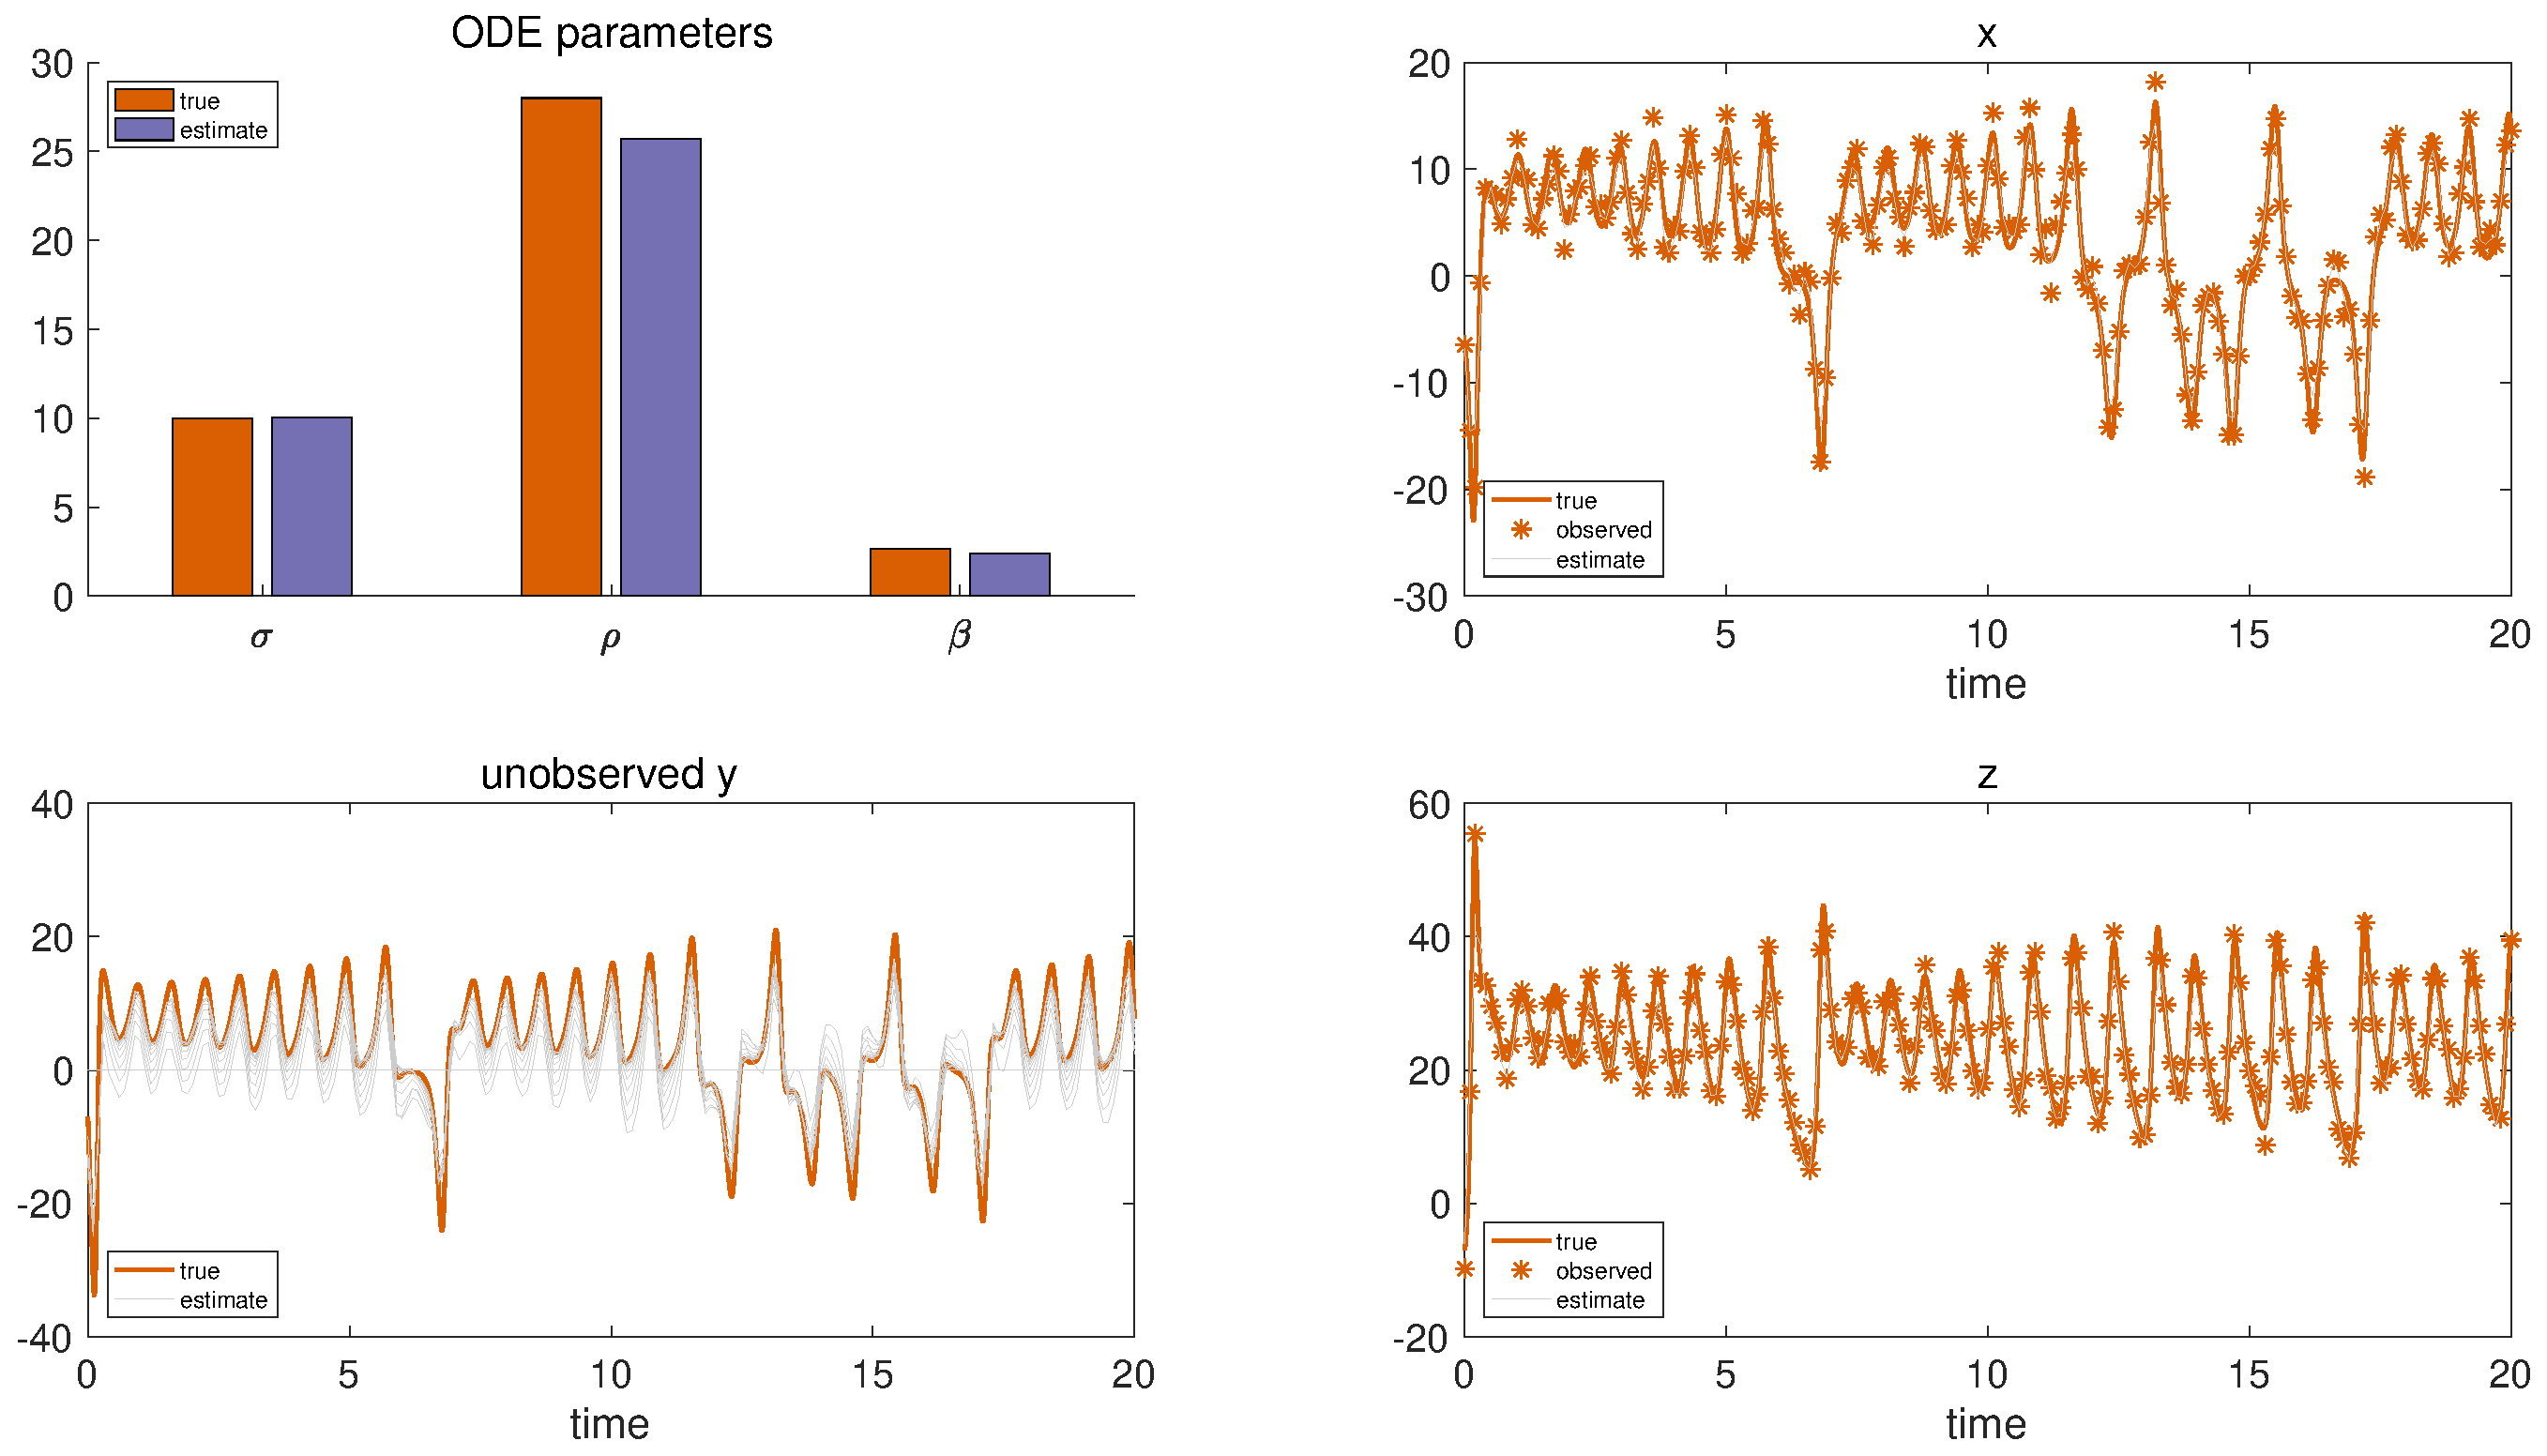
\includegraphics [width=5in]{Lorenz_attractor_4_23.eps}

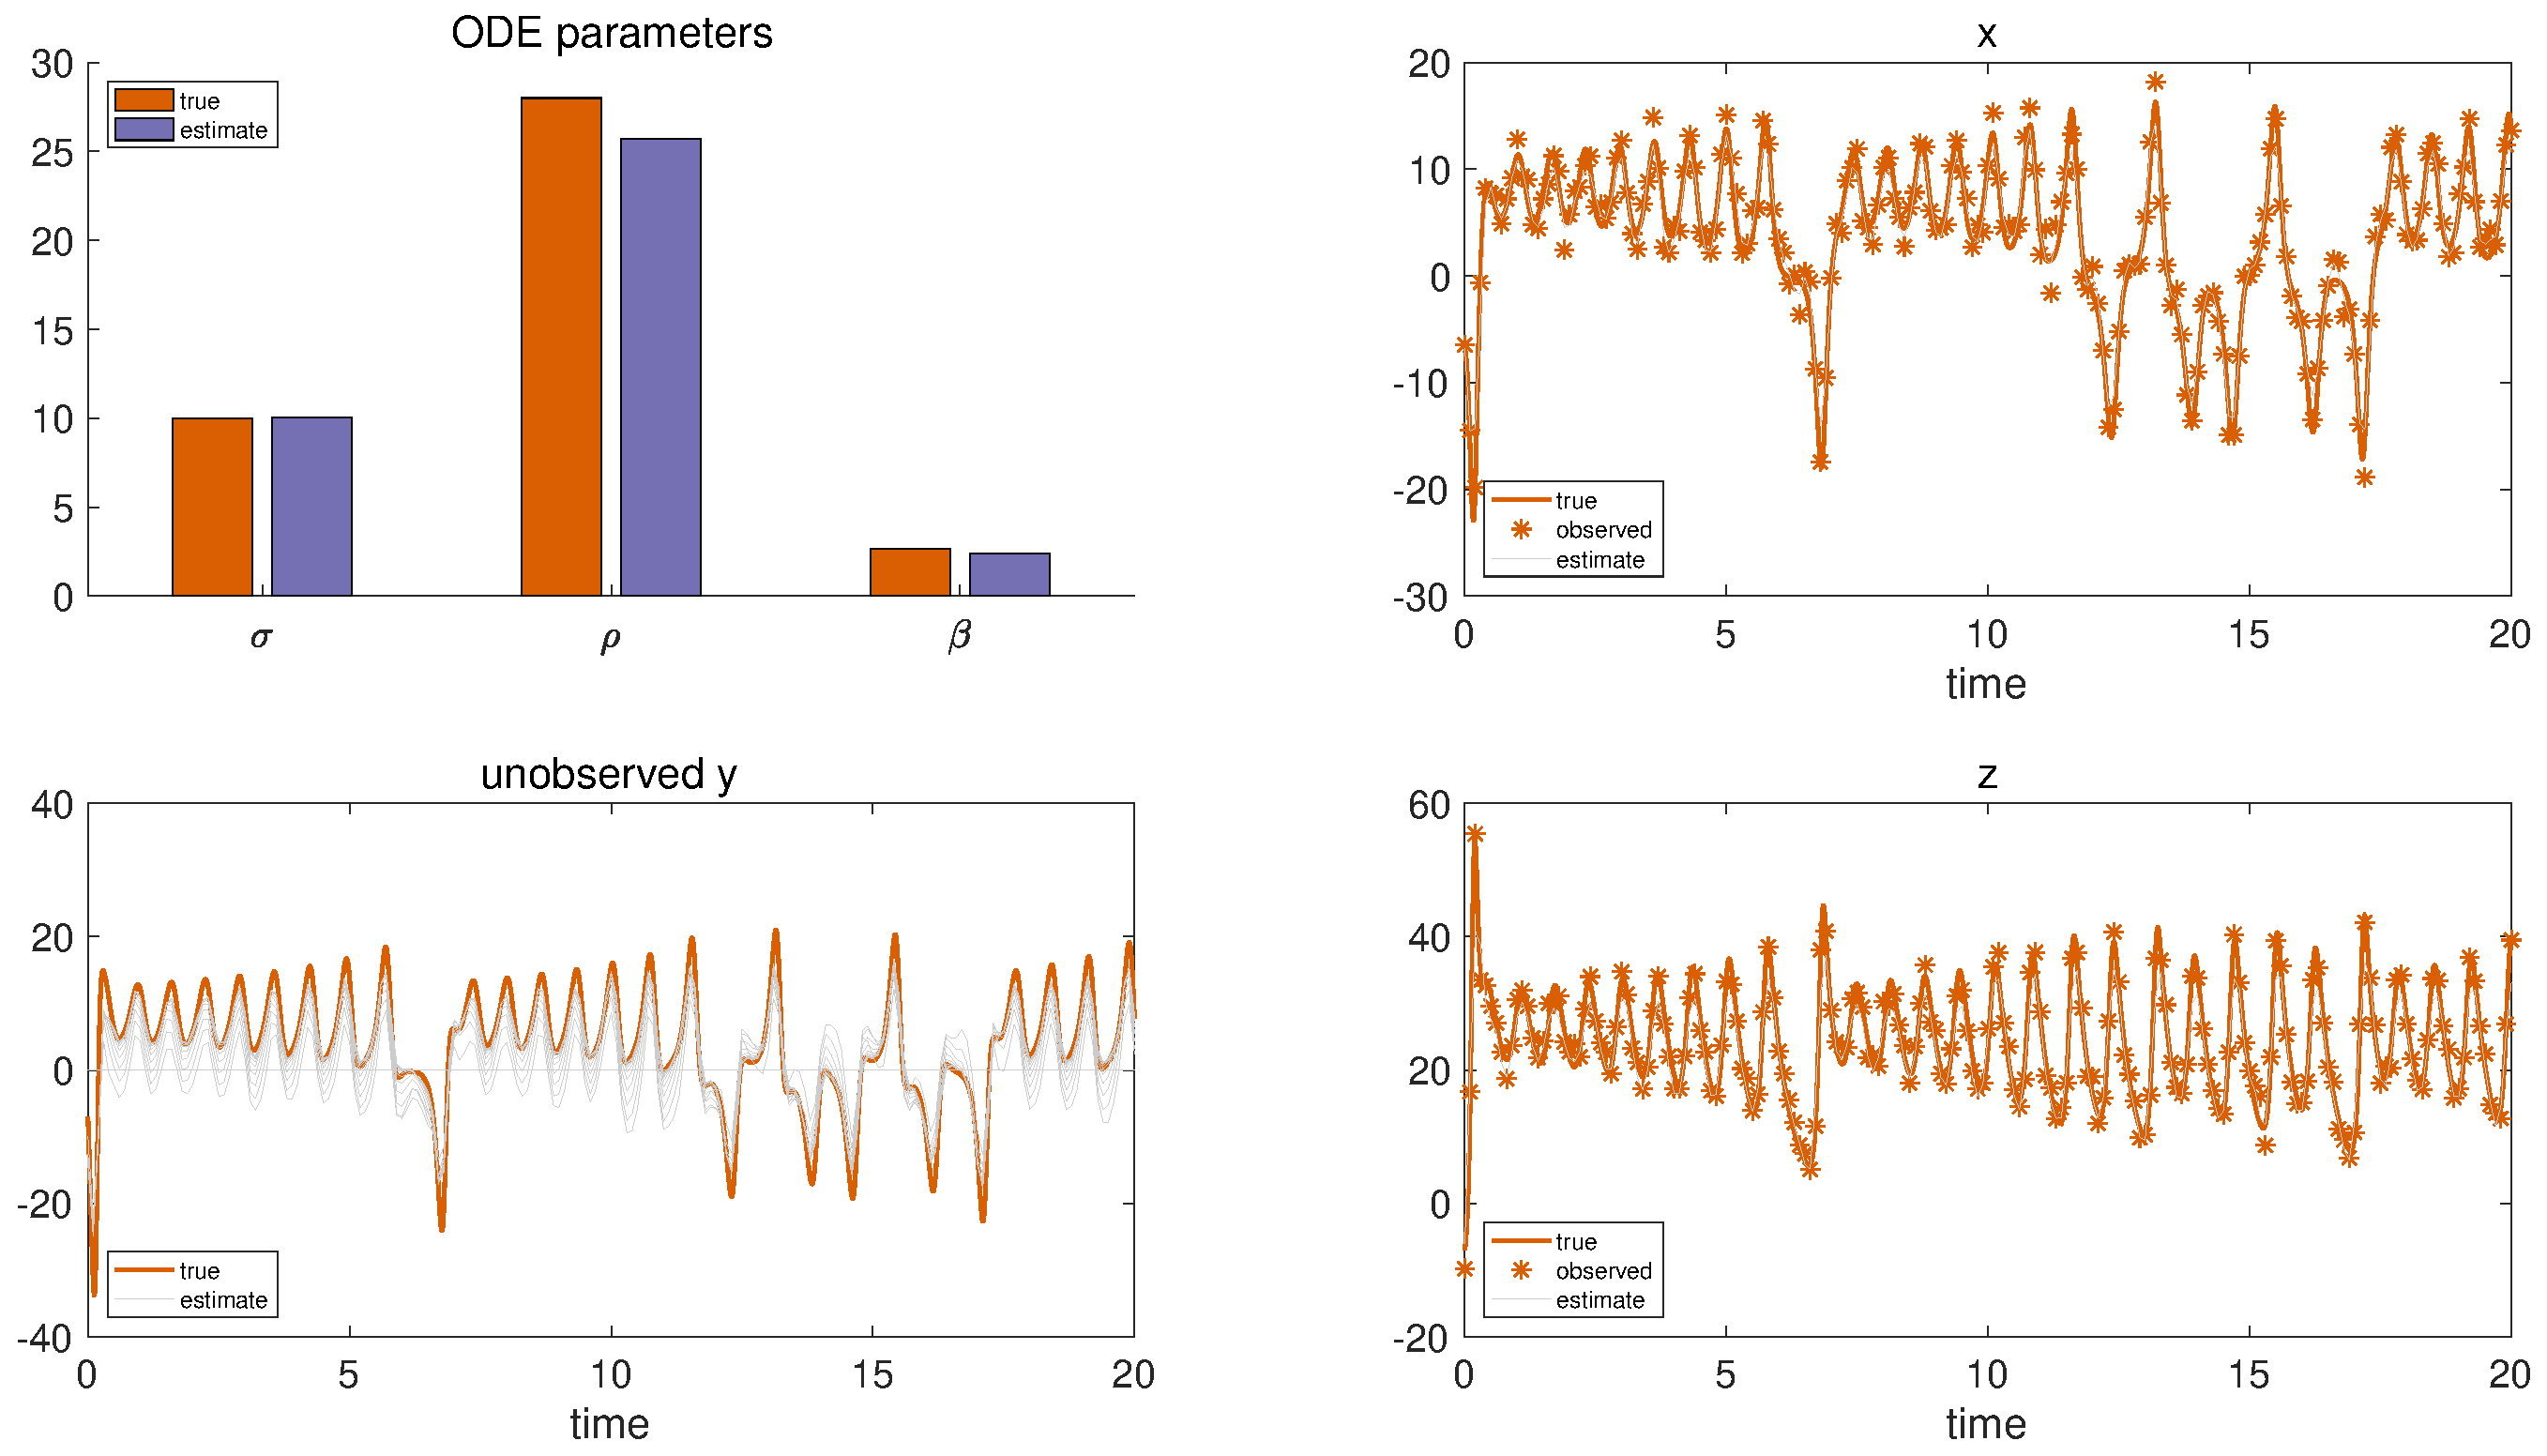
\includegraphics [width=5in]{Lorenz_attractor_4_24.eps}

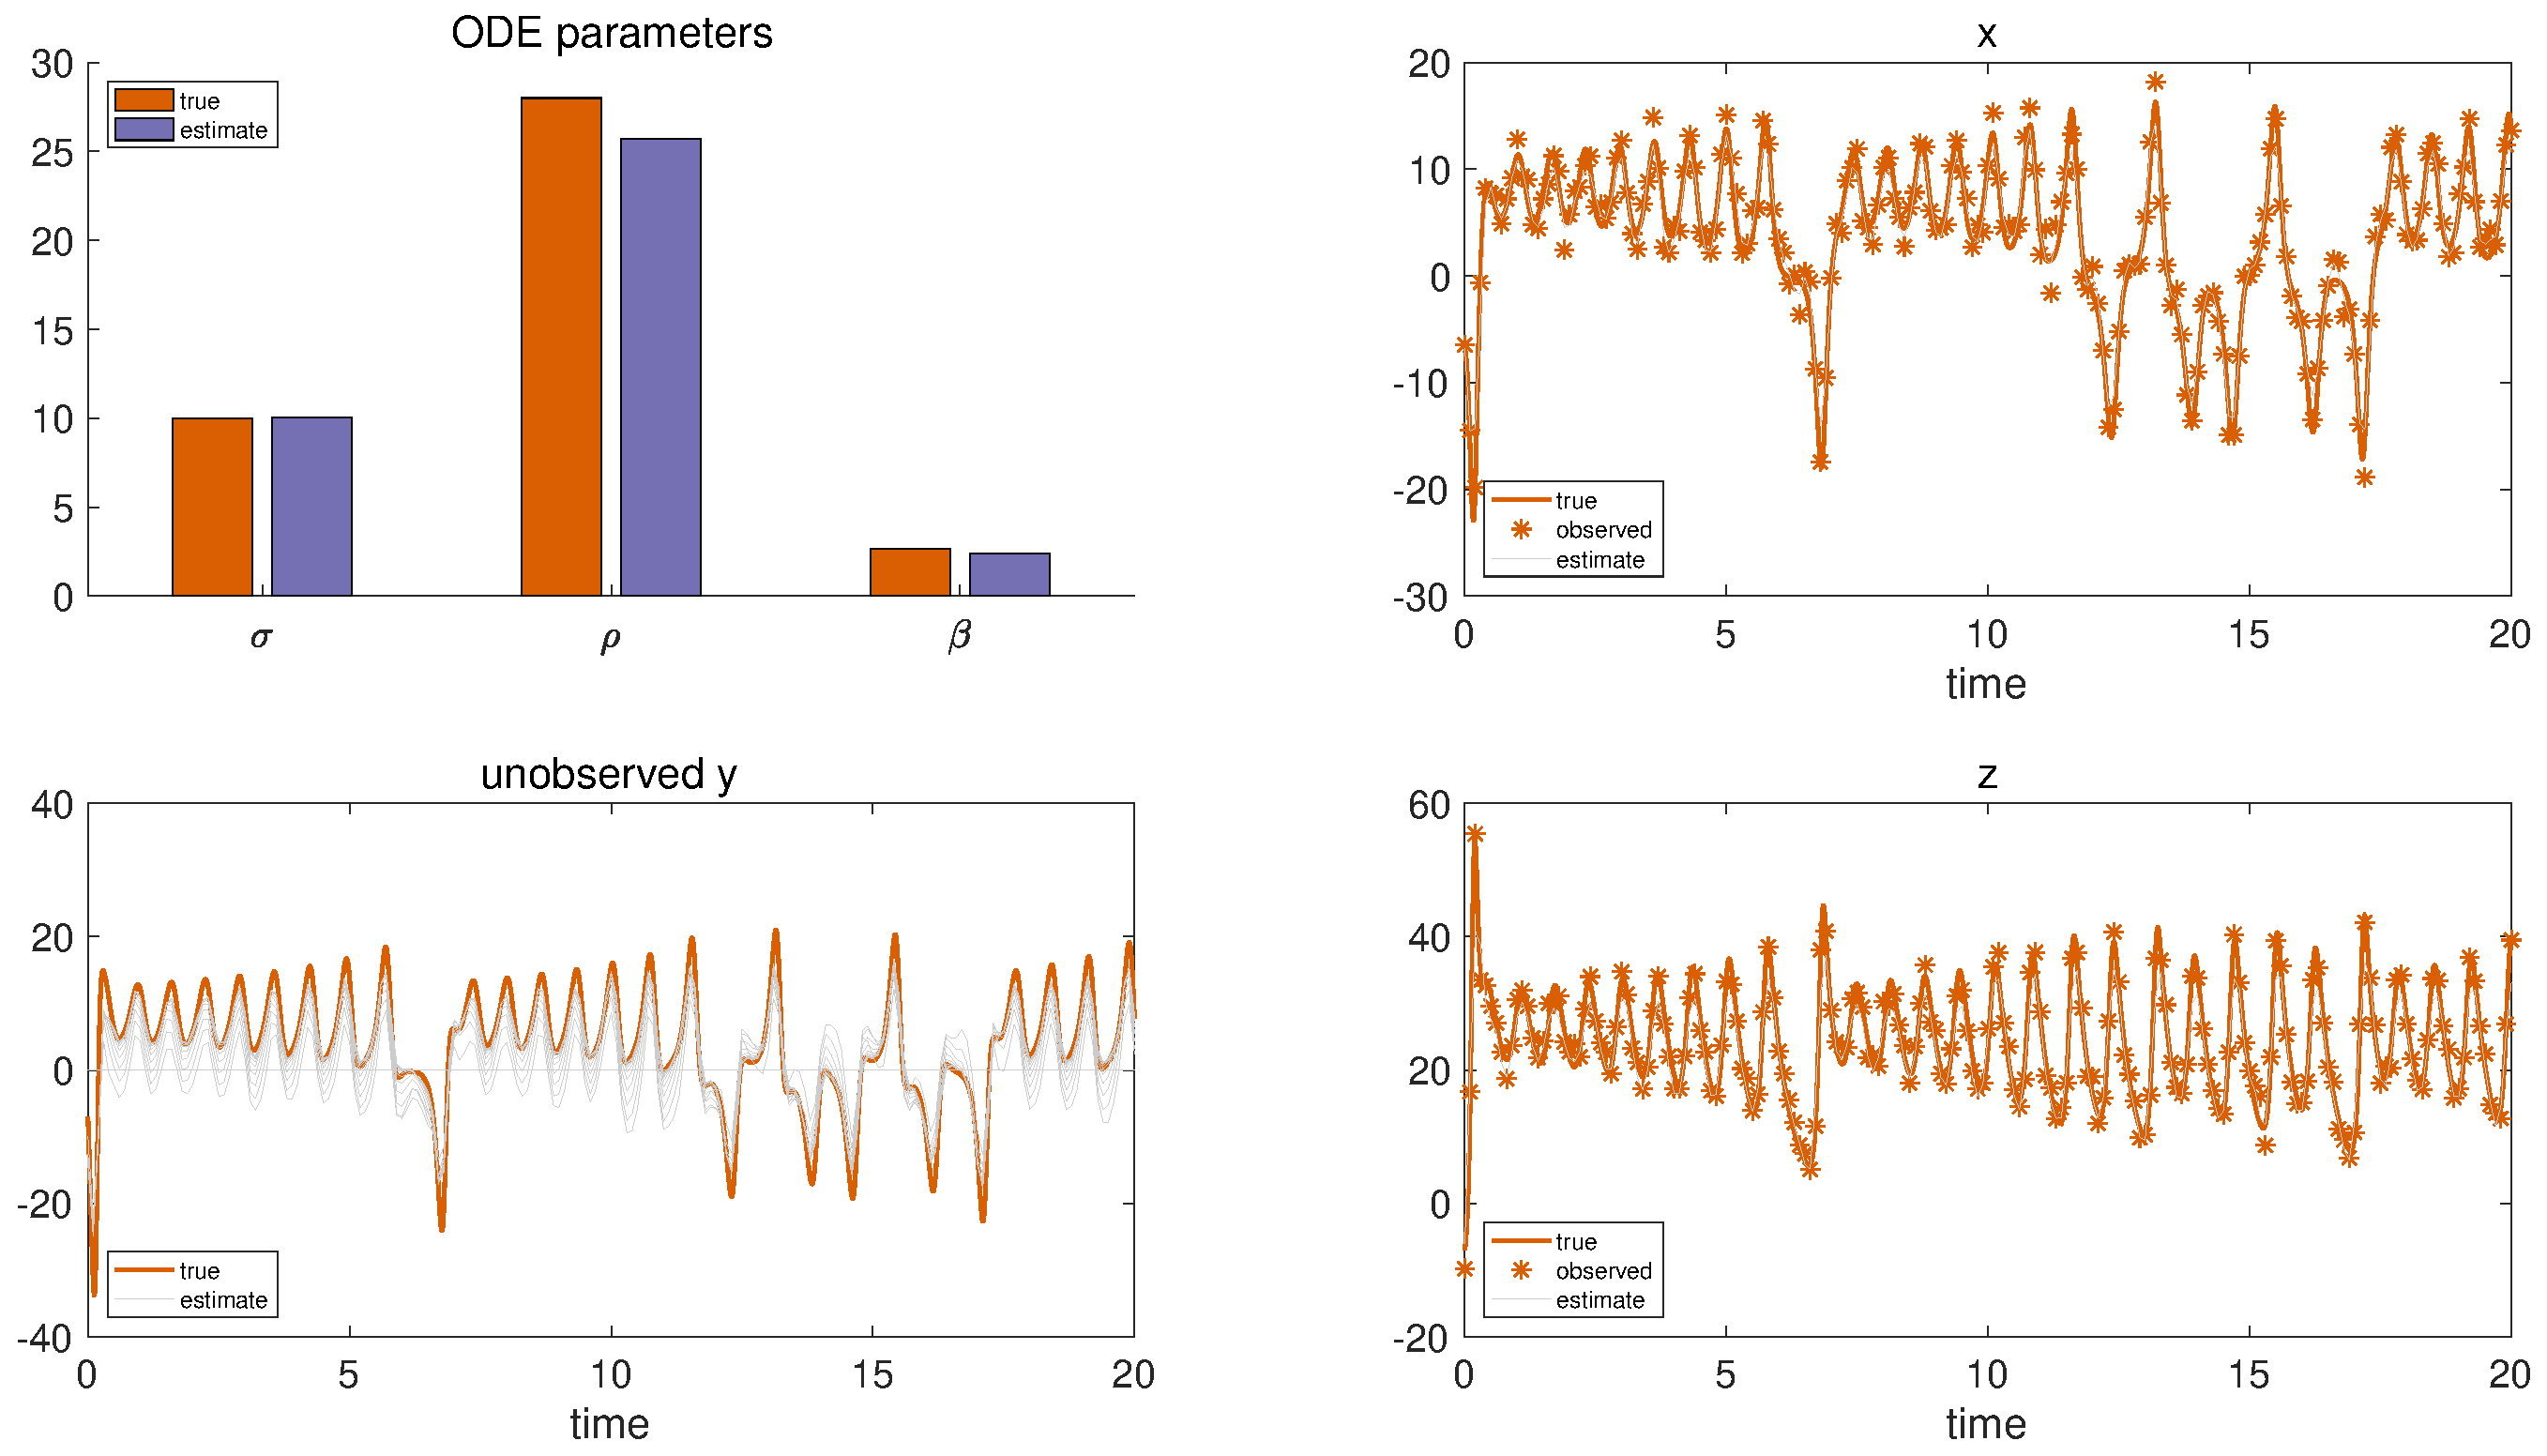
\includegraphics [width=5in]{Lorenz_attractor_4_25.eps}

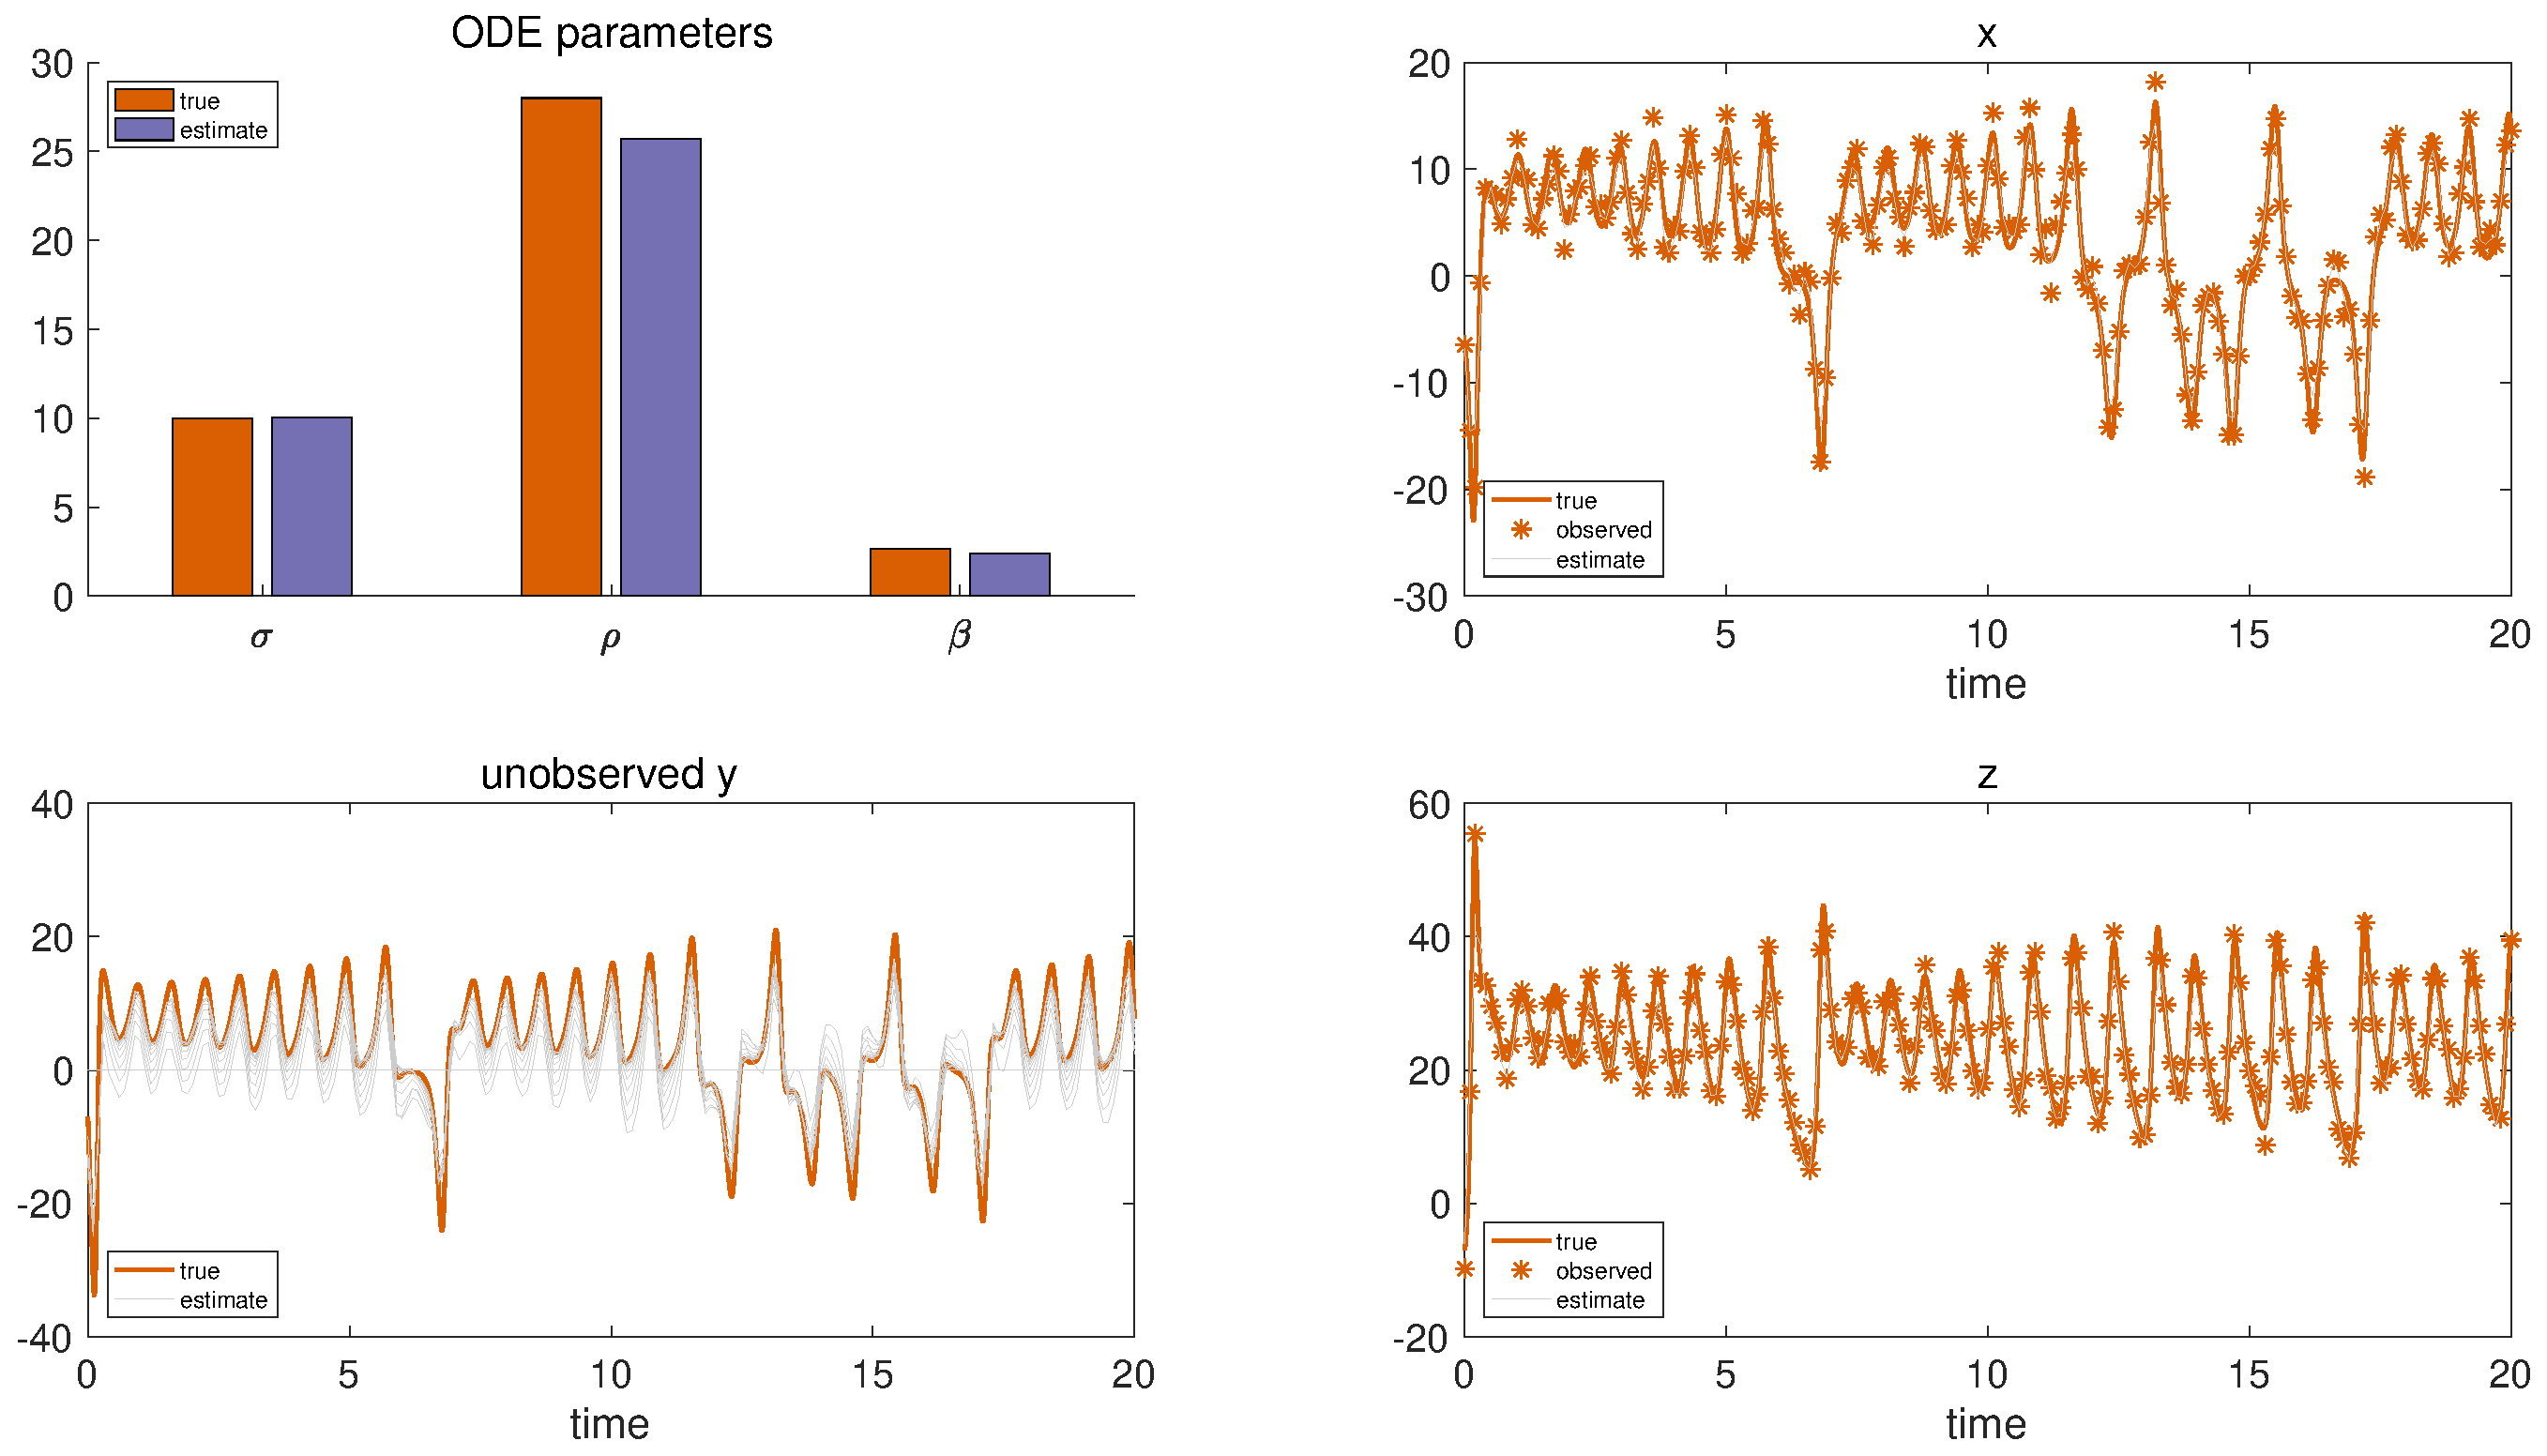
\includegraphics [width=5in]{Lorenz_attractor_4_26.eps}

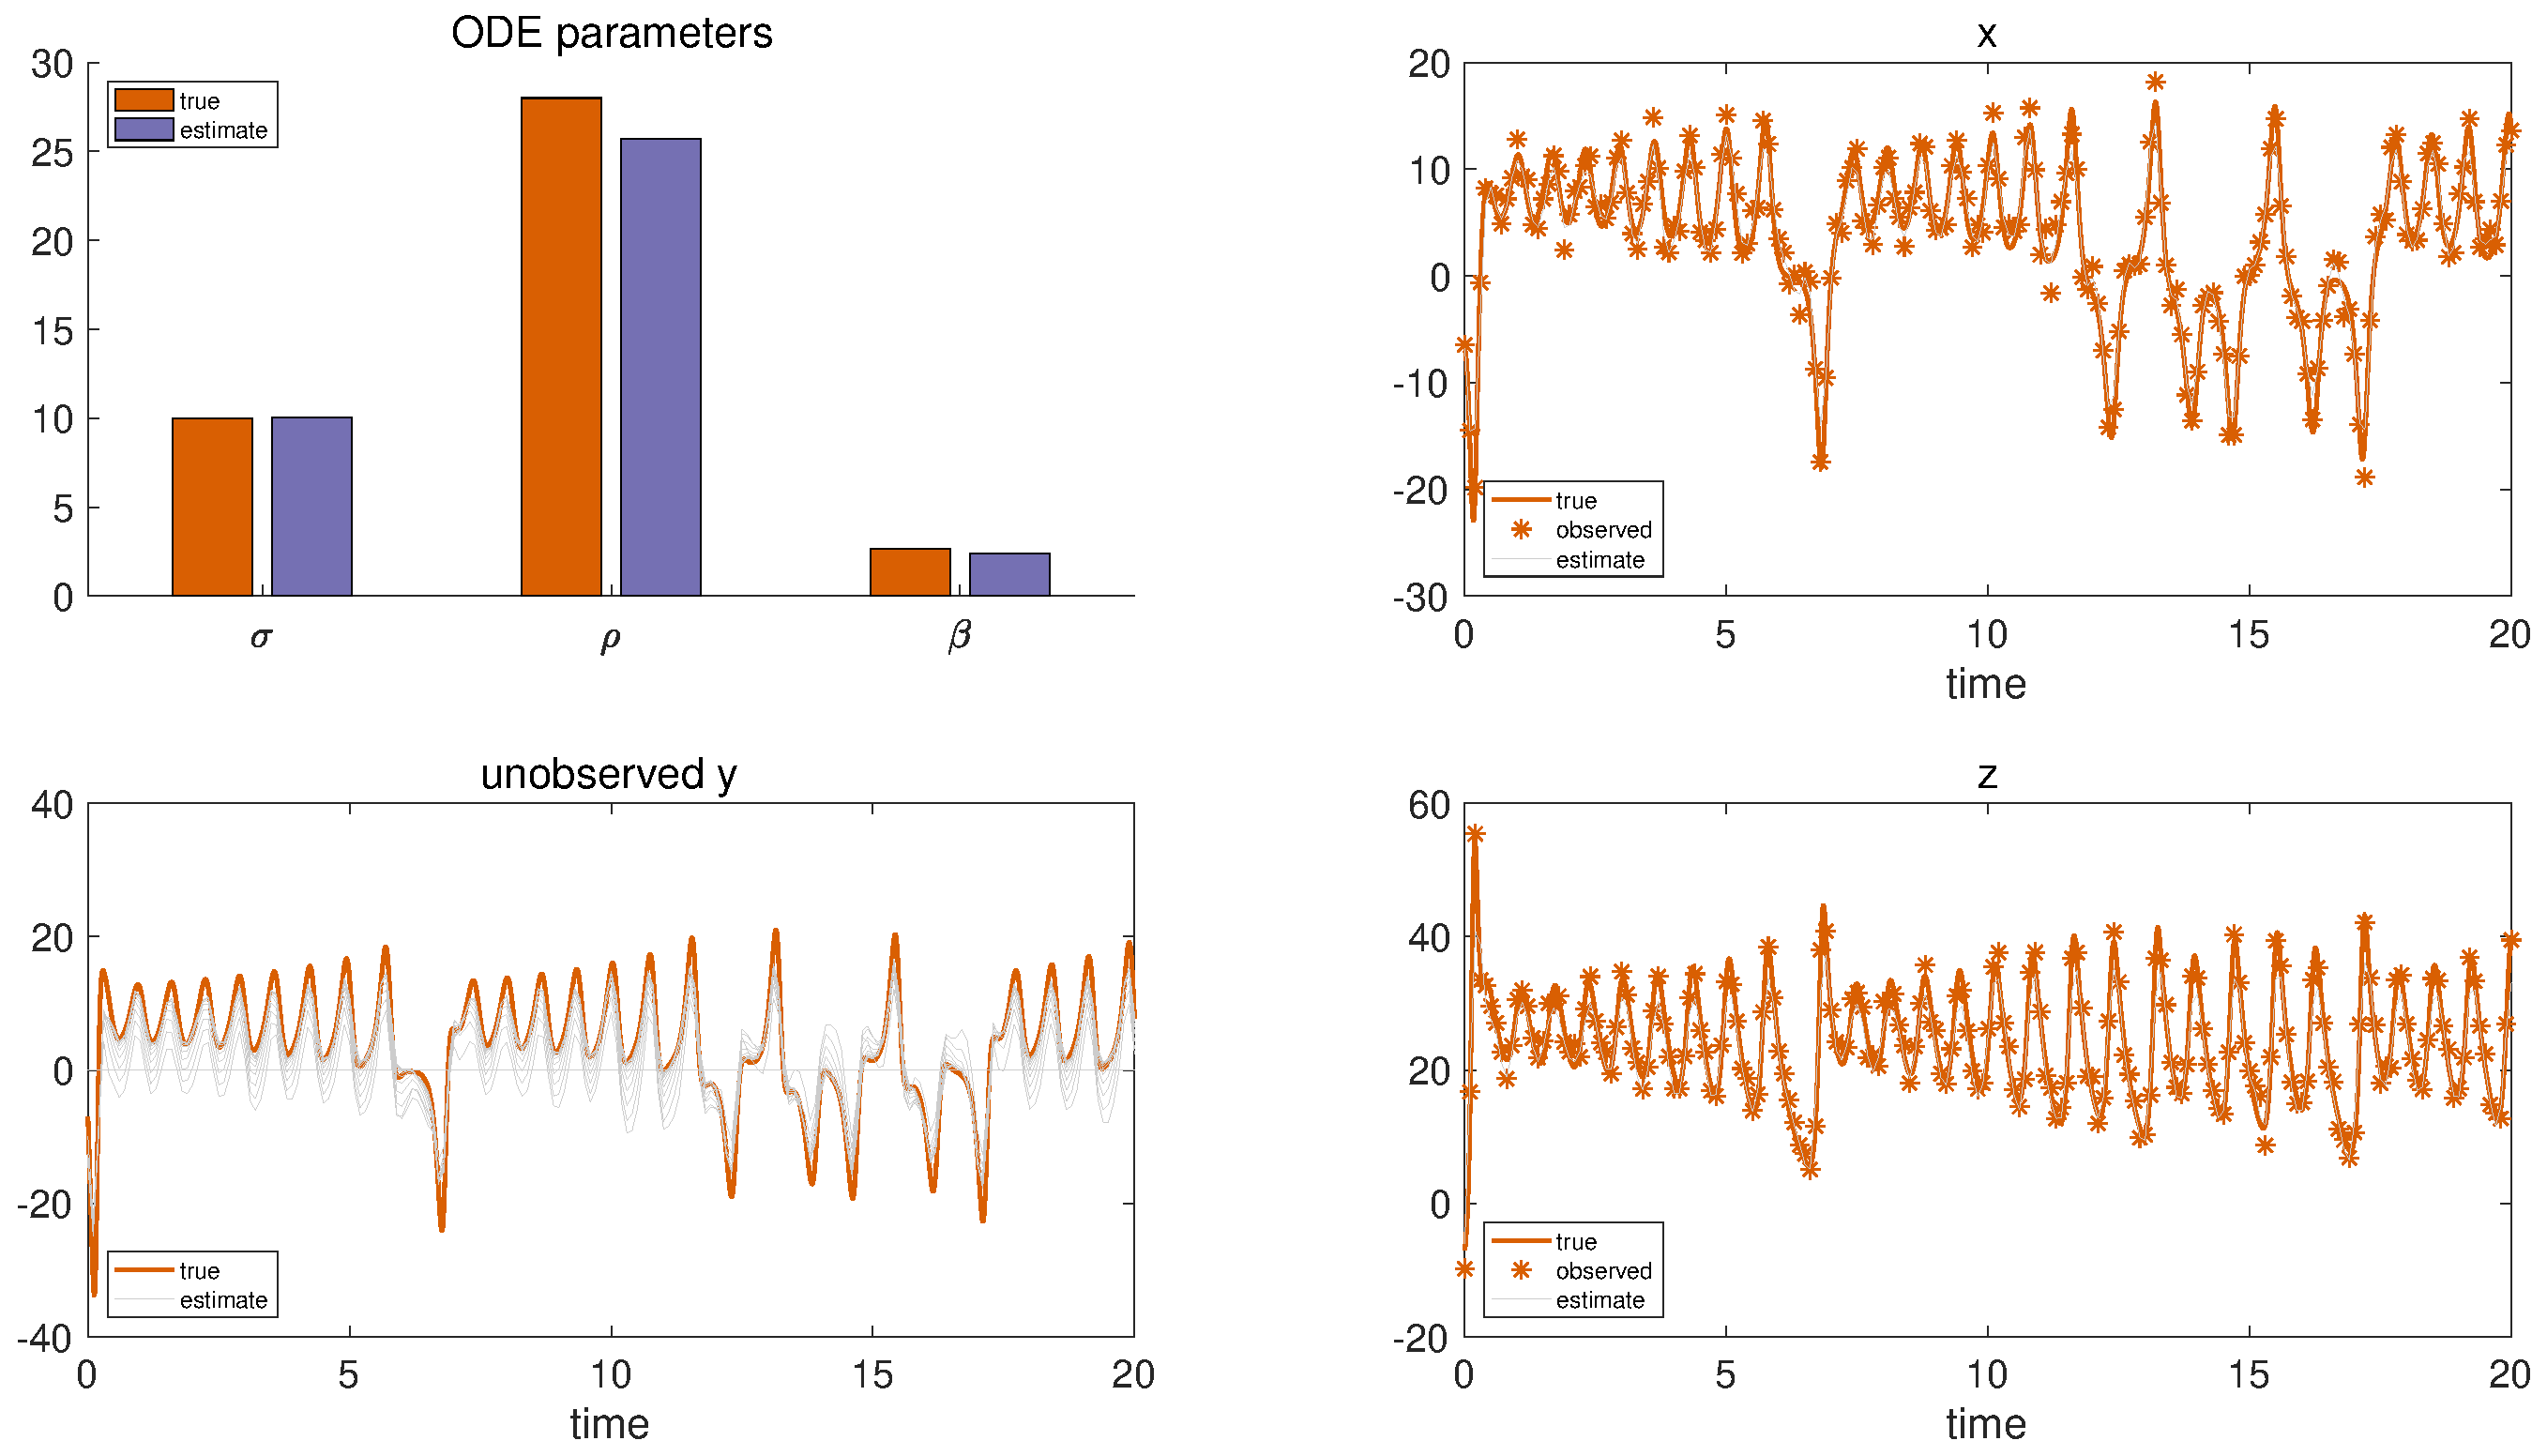
\includegraphics [width=5in]{Lorenz_attractor_4_27.eps}

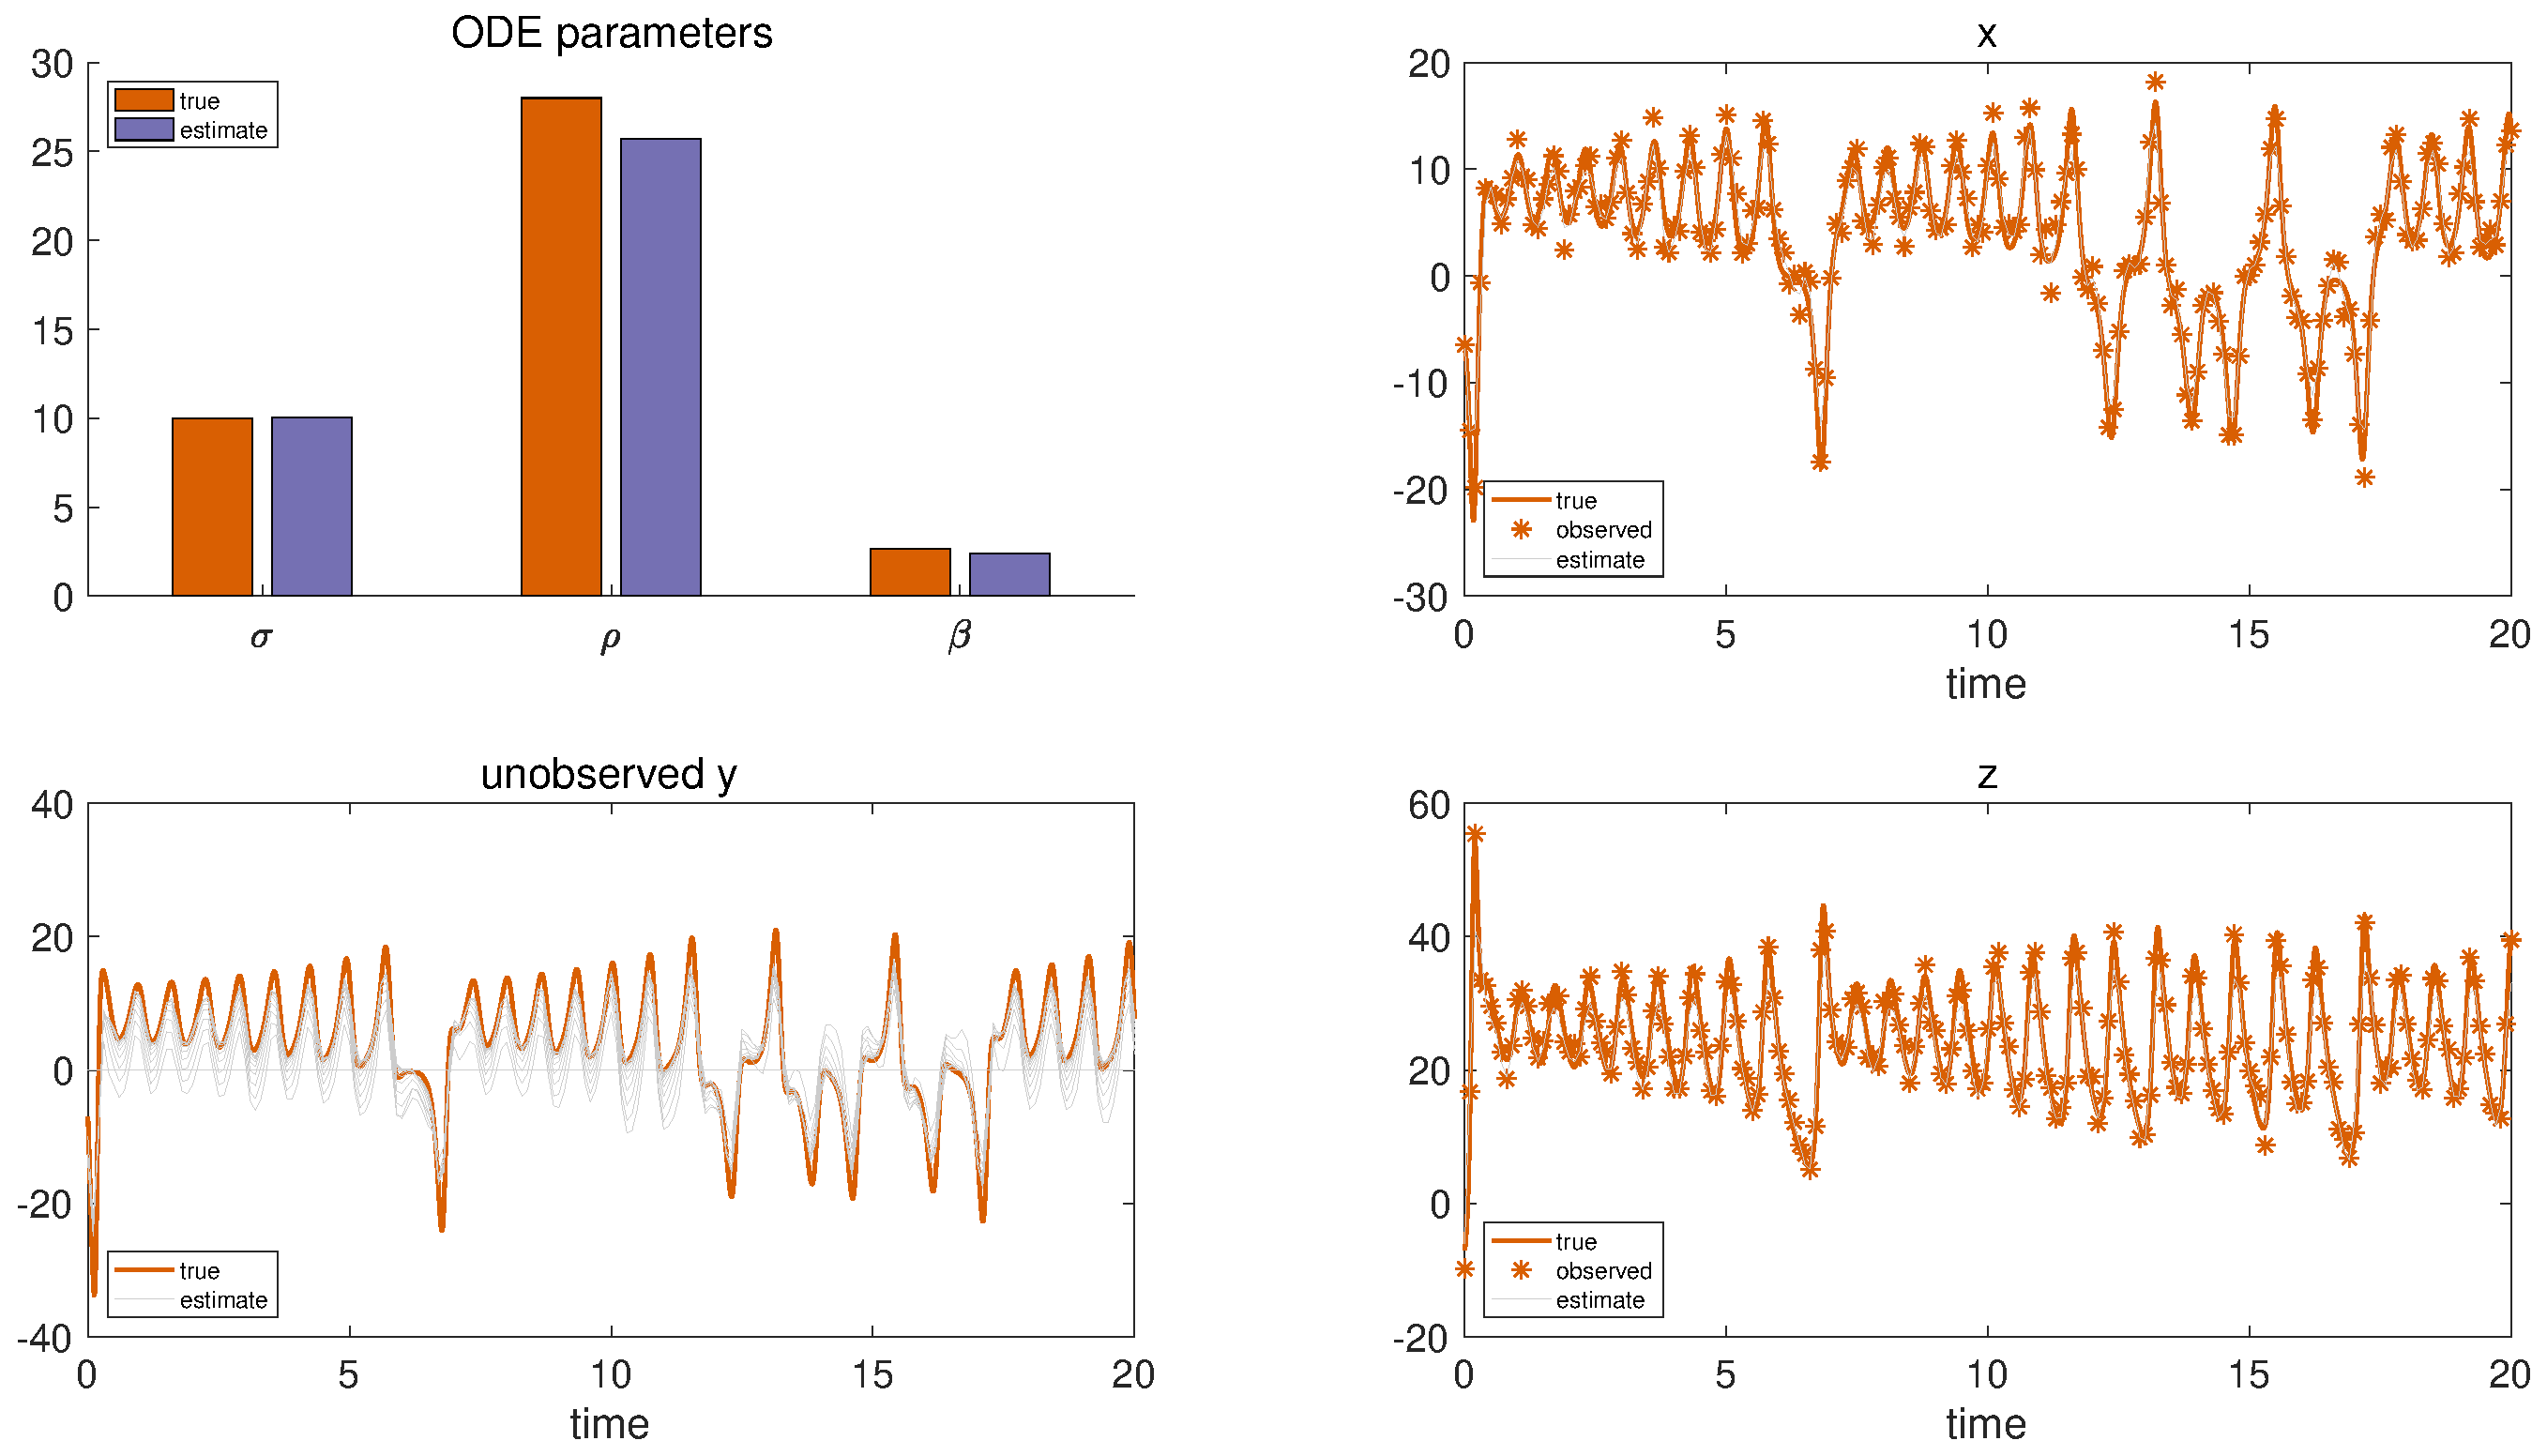
\includegraphics [width=5in]{Lorenz_attractor_4_28.eps}

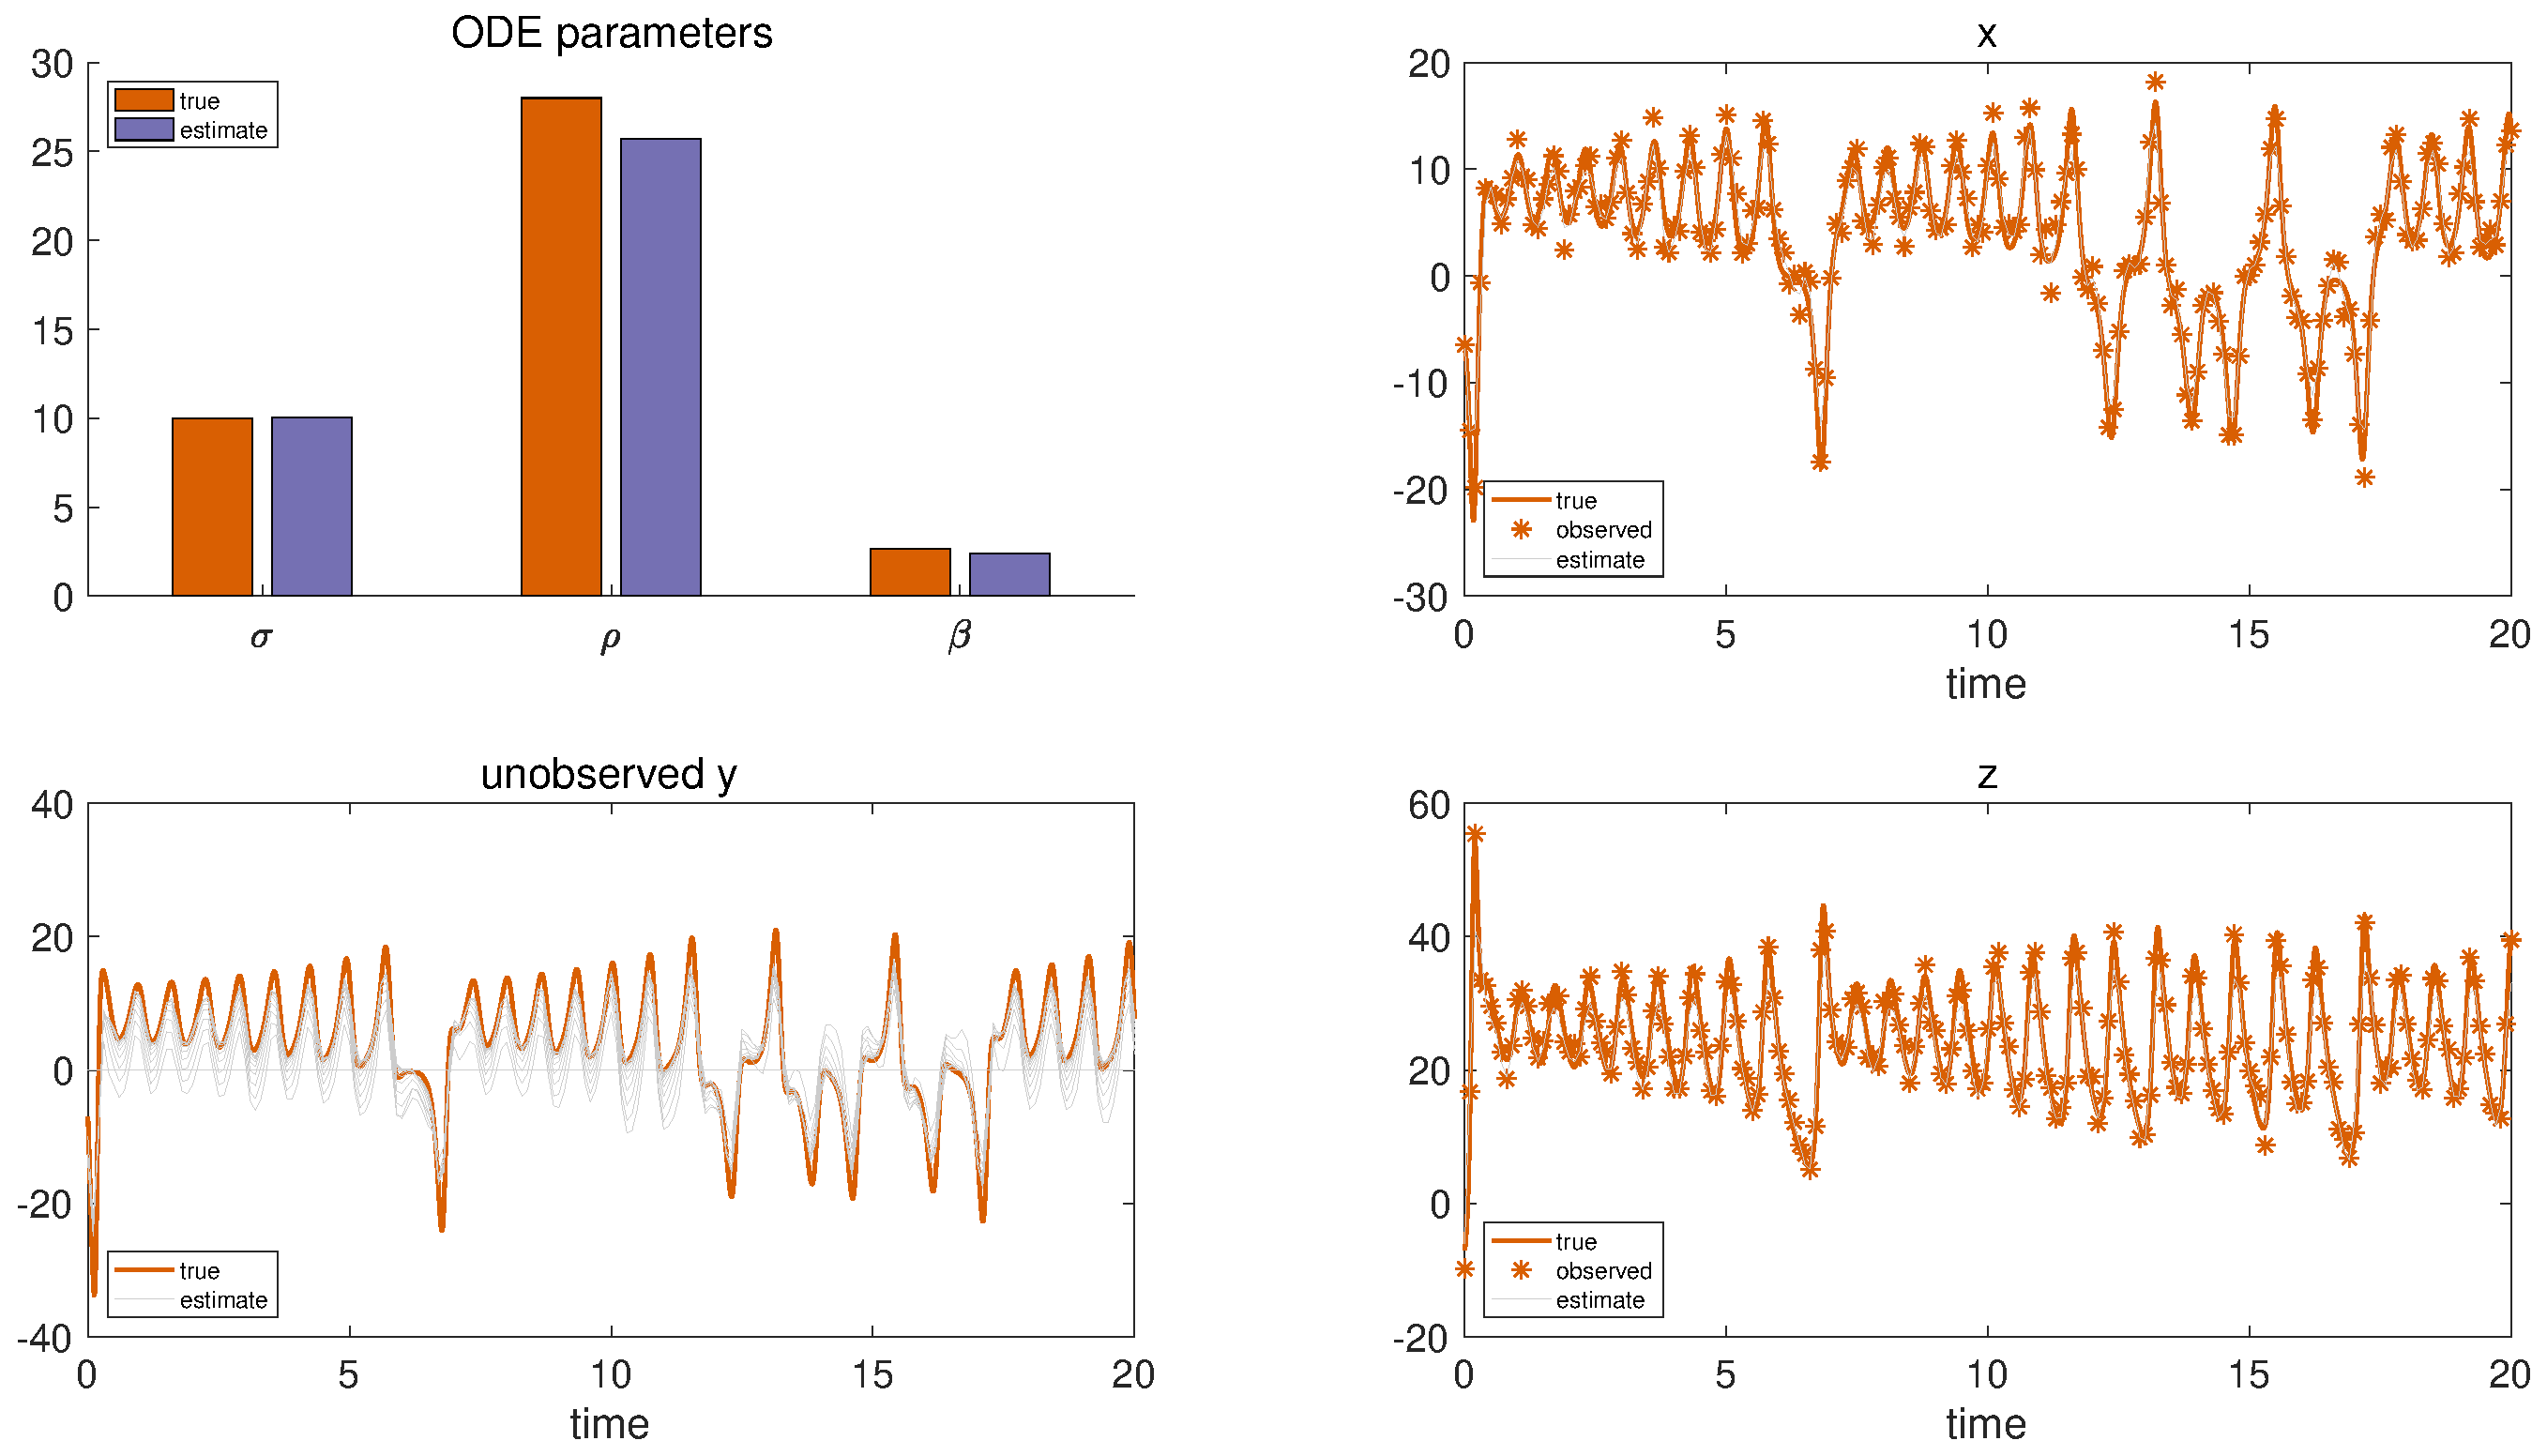
\includegraphics [width=5in]{Lorenz_attractor_4_29.eps}

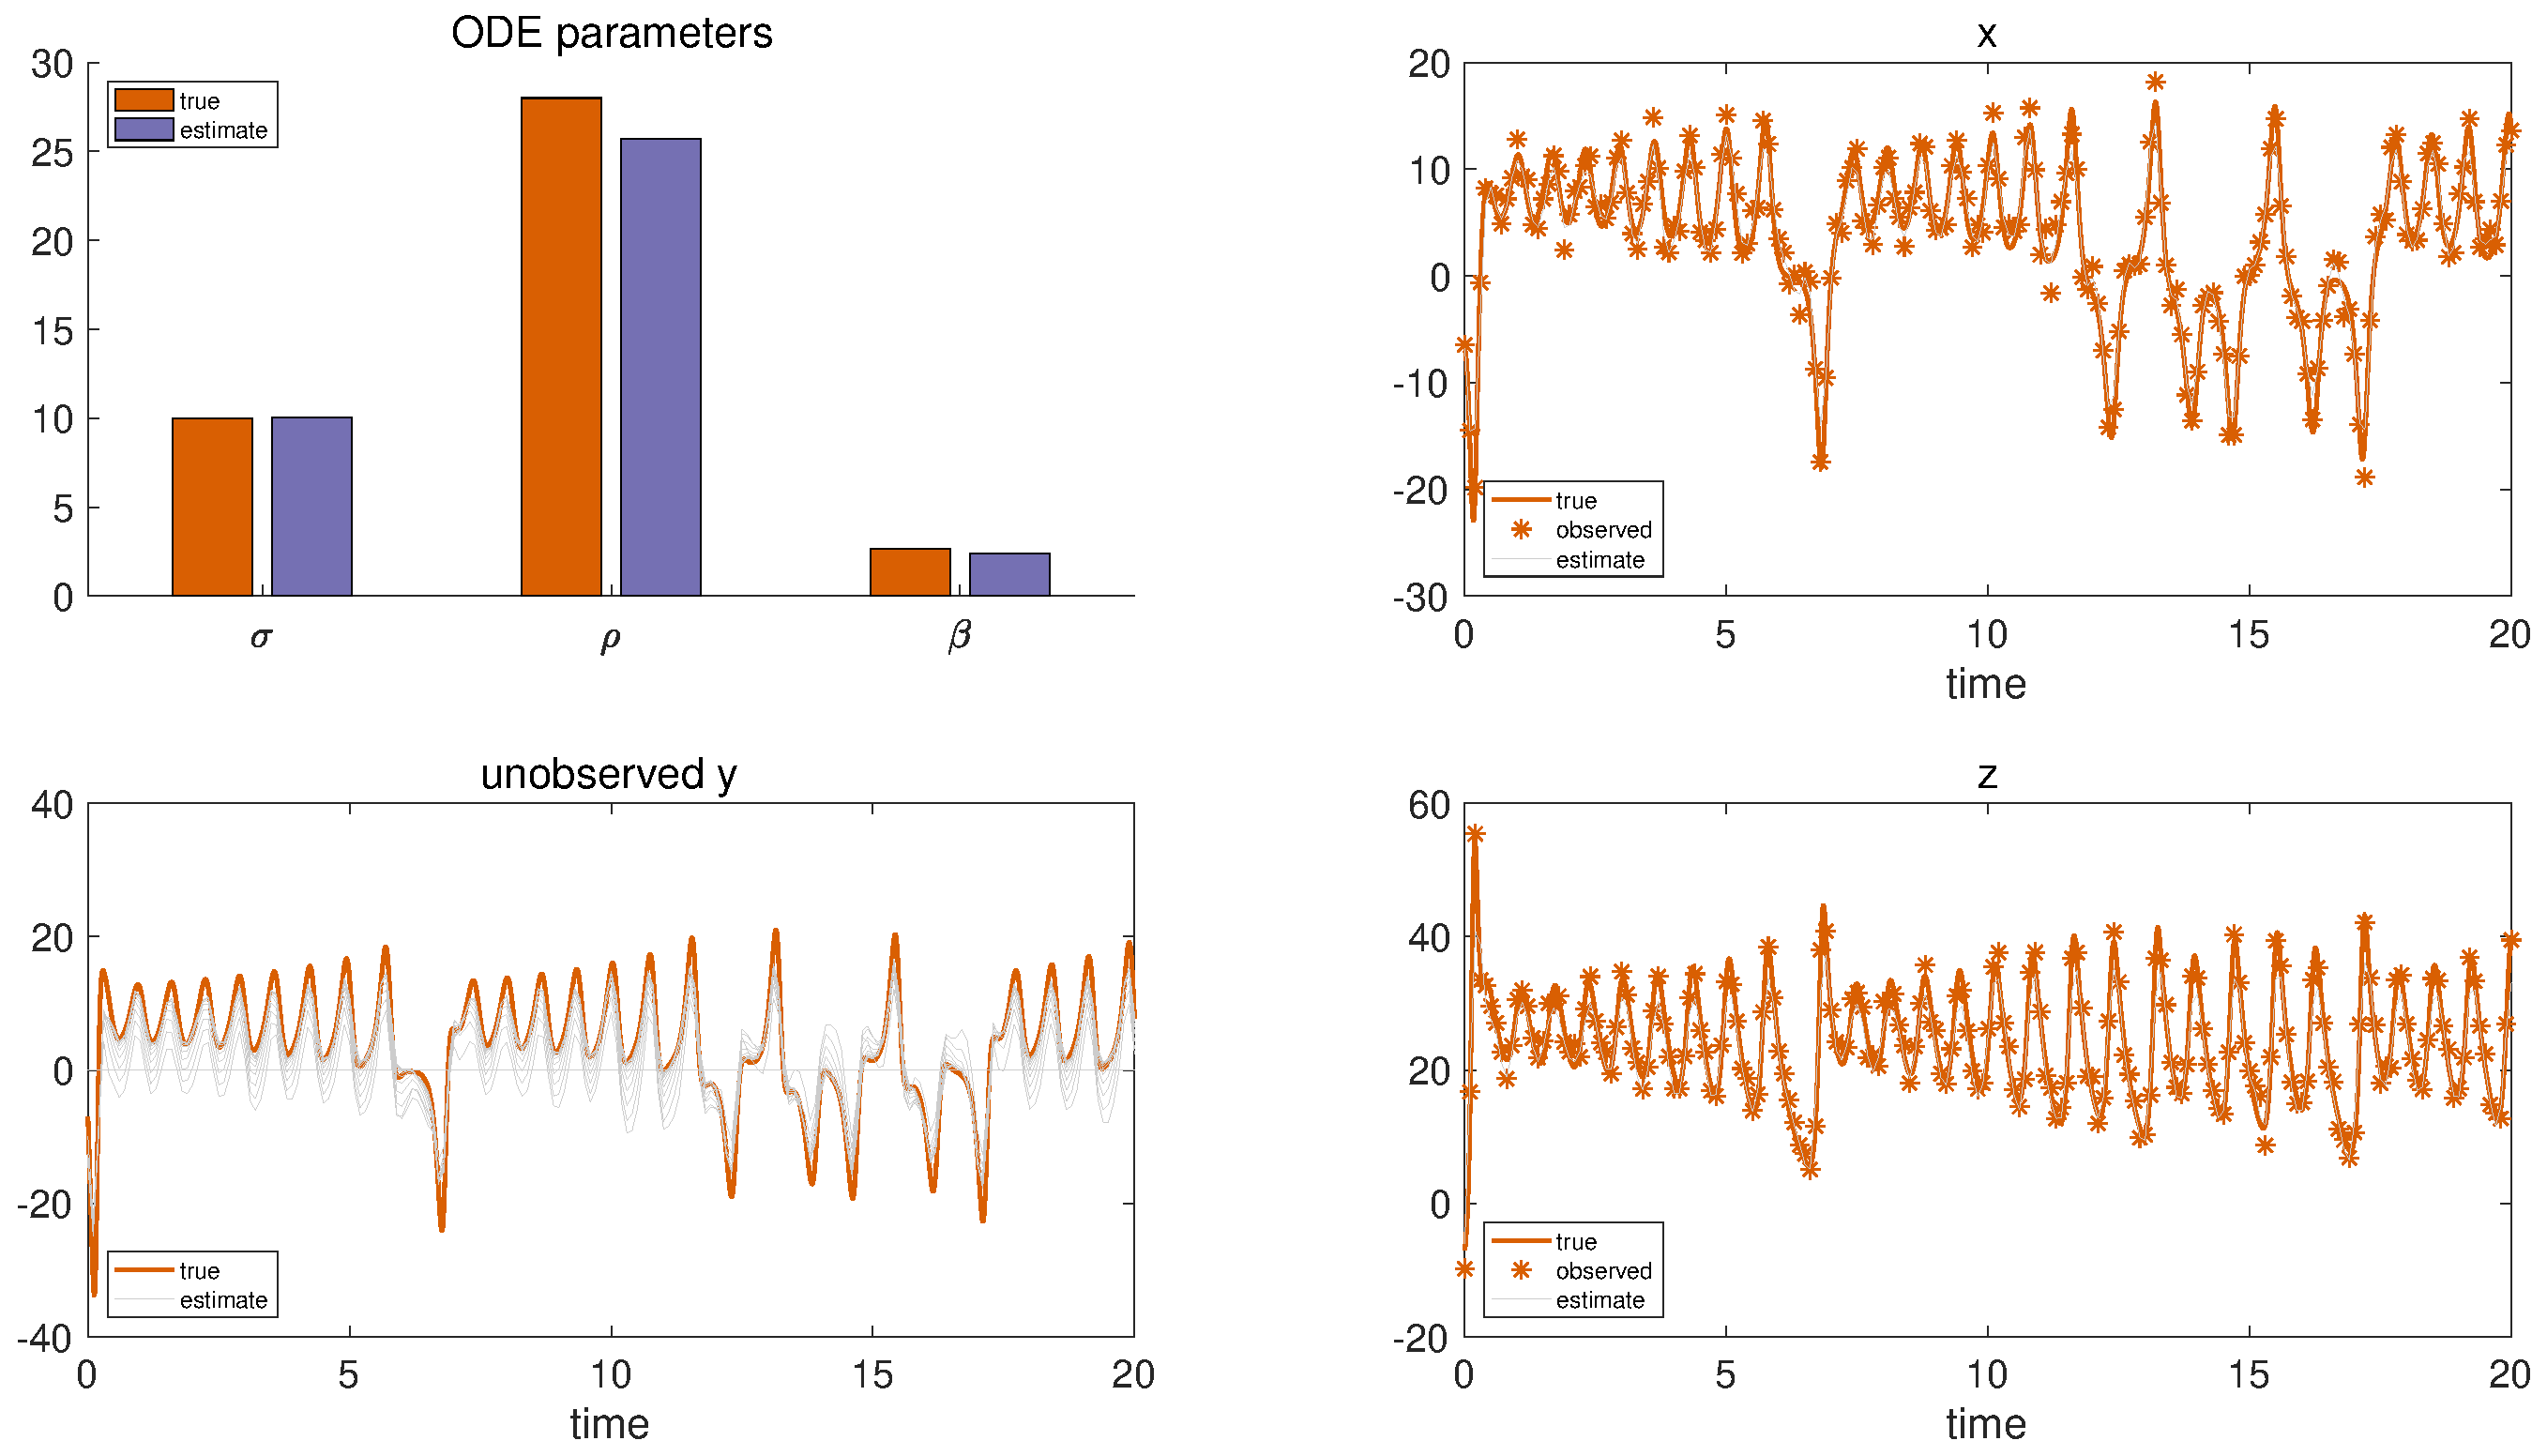
\includegraphics [width=5in]{Lorenz_attractor_4_30.eps}

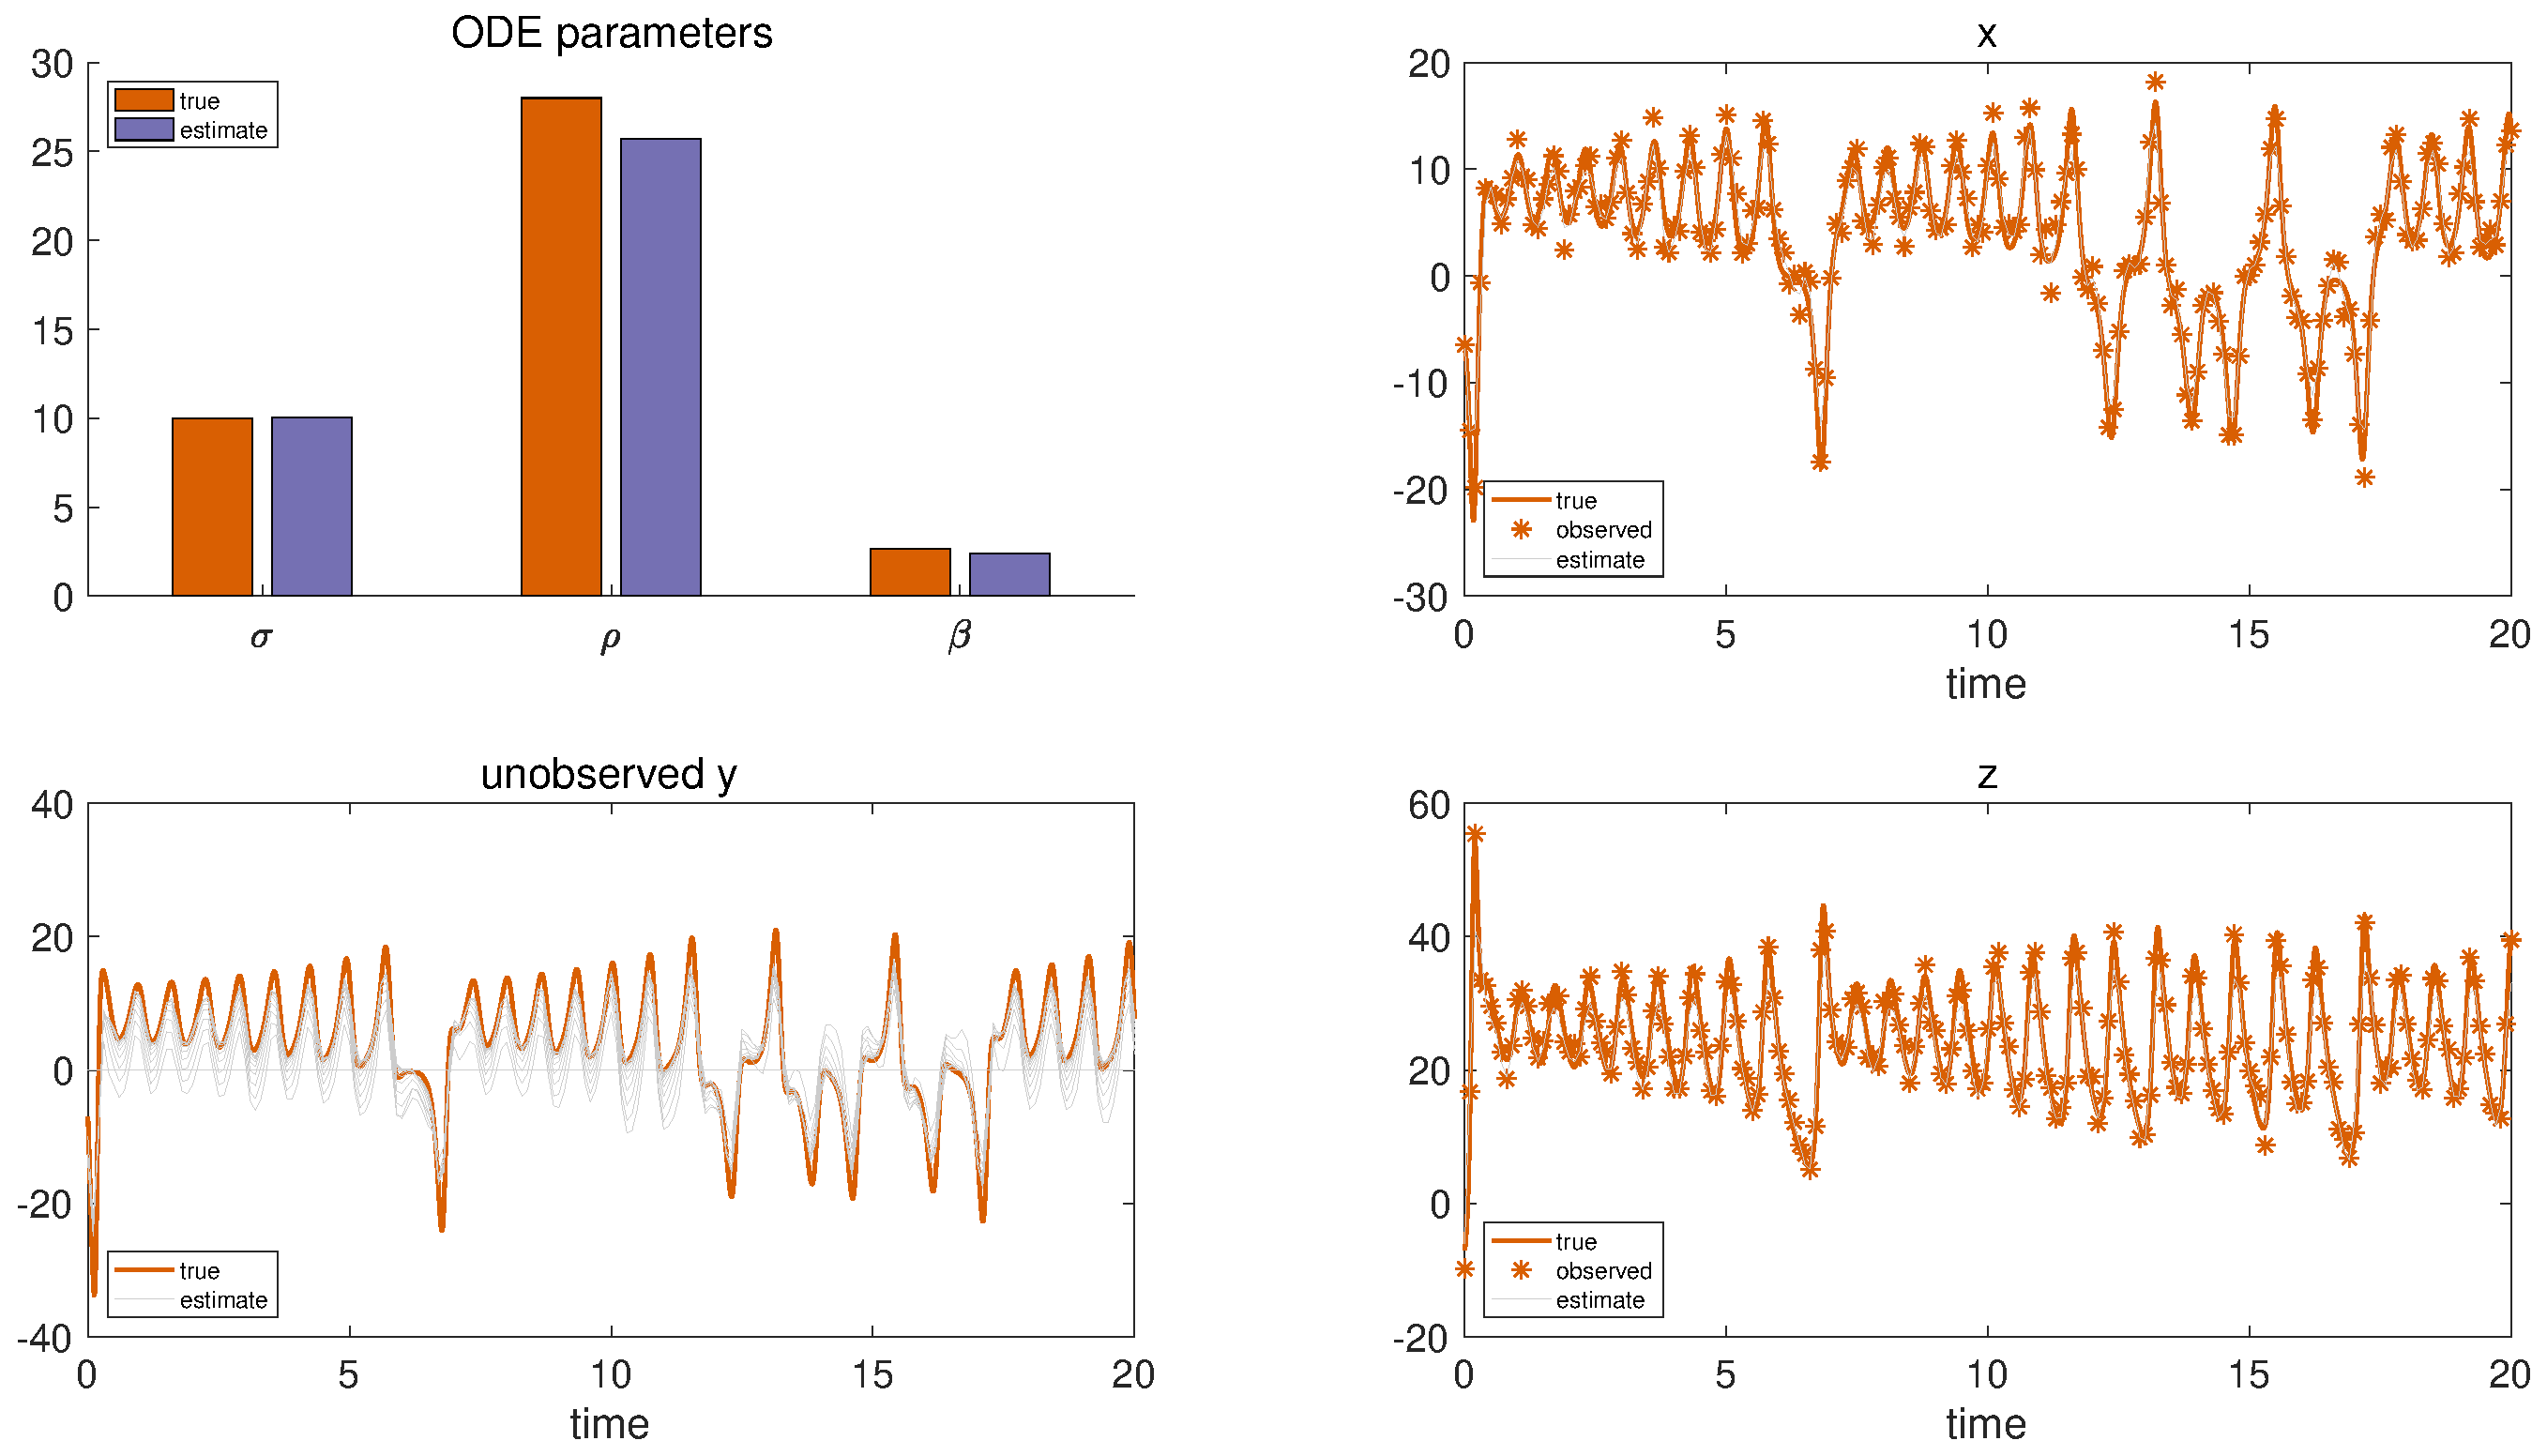
\includegraphics [width=5in]{Lorenz_attractor_4_31.eps}

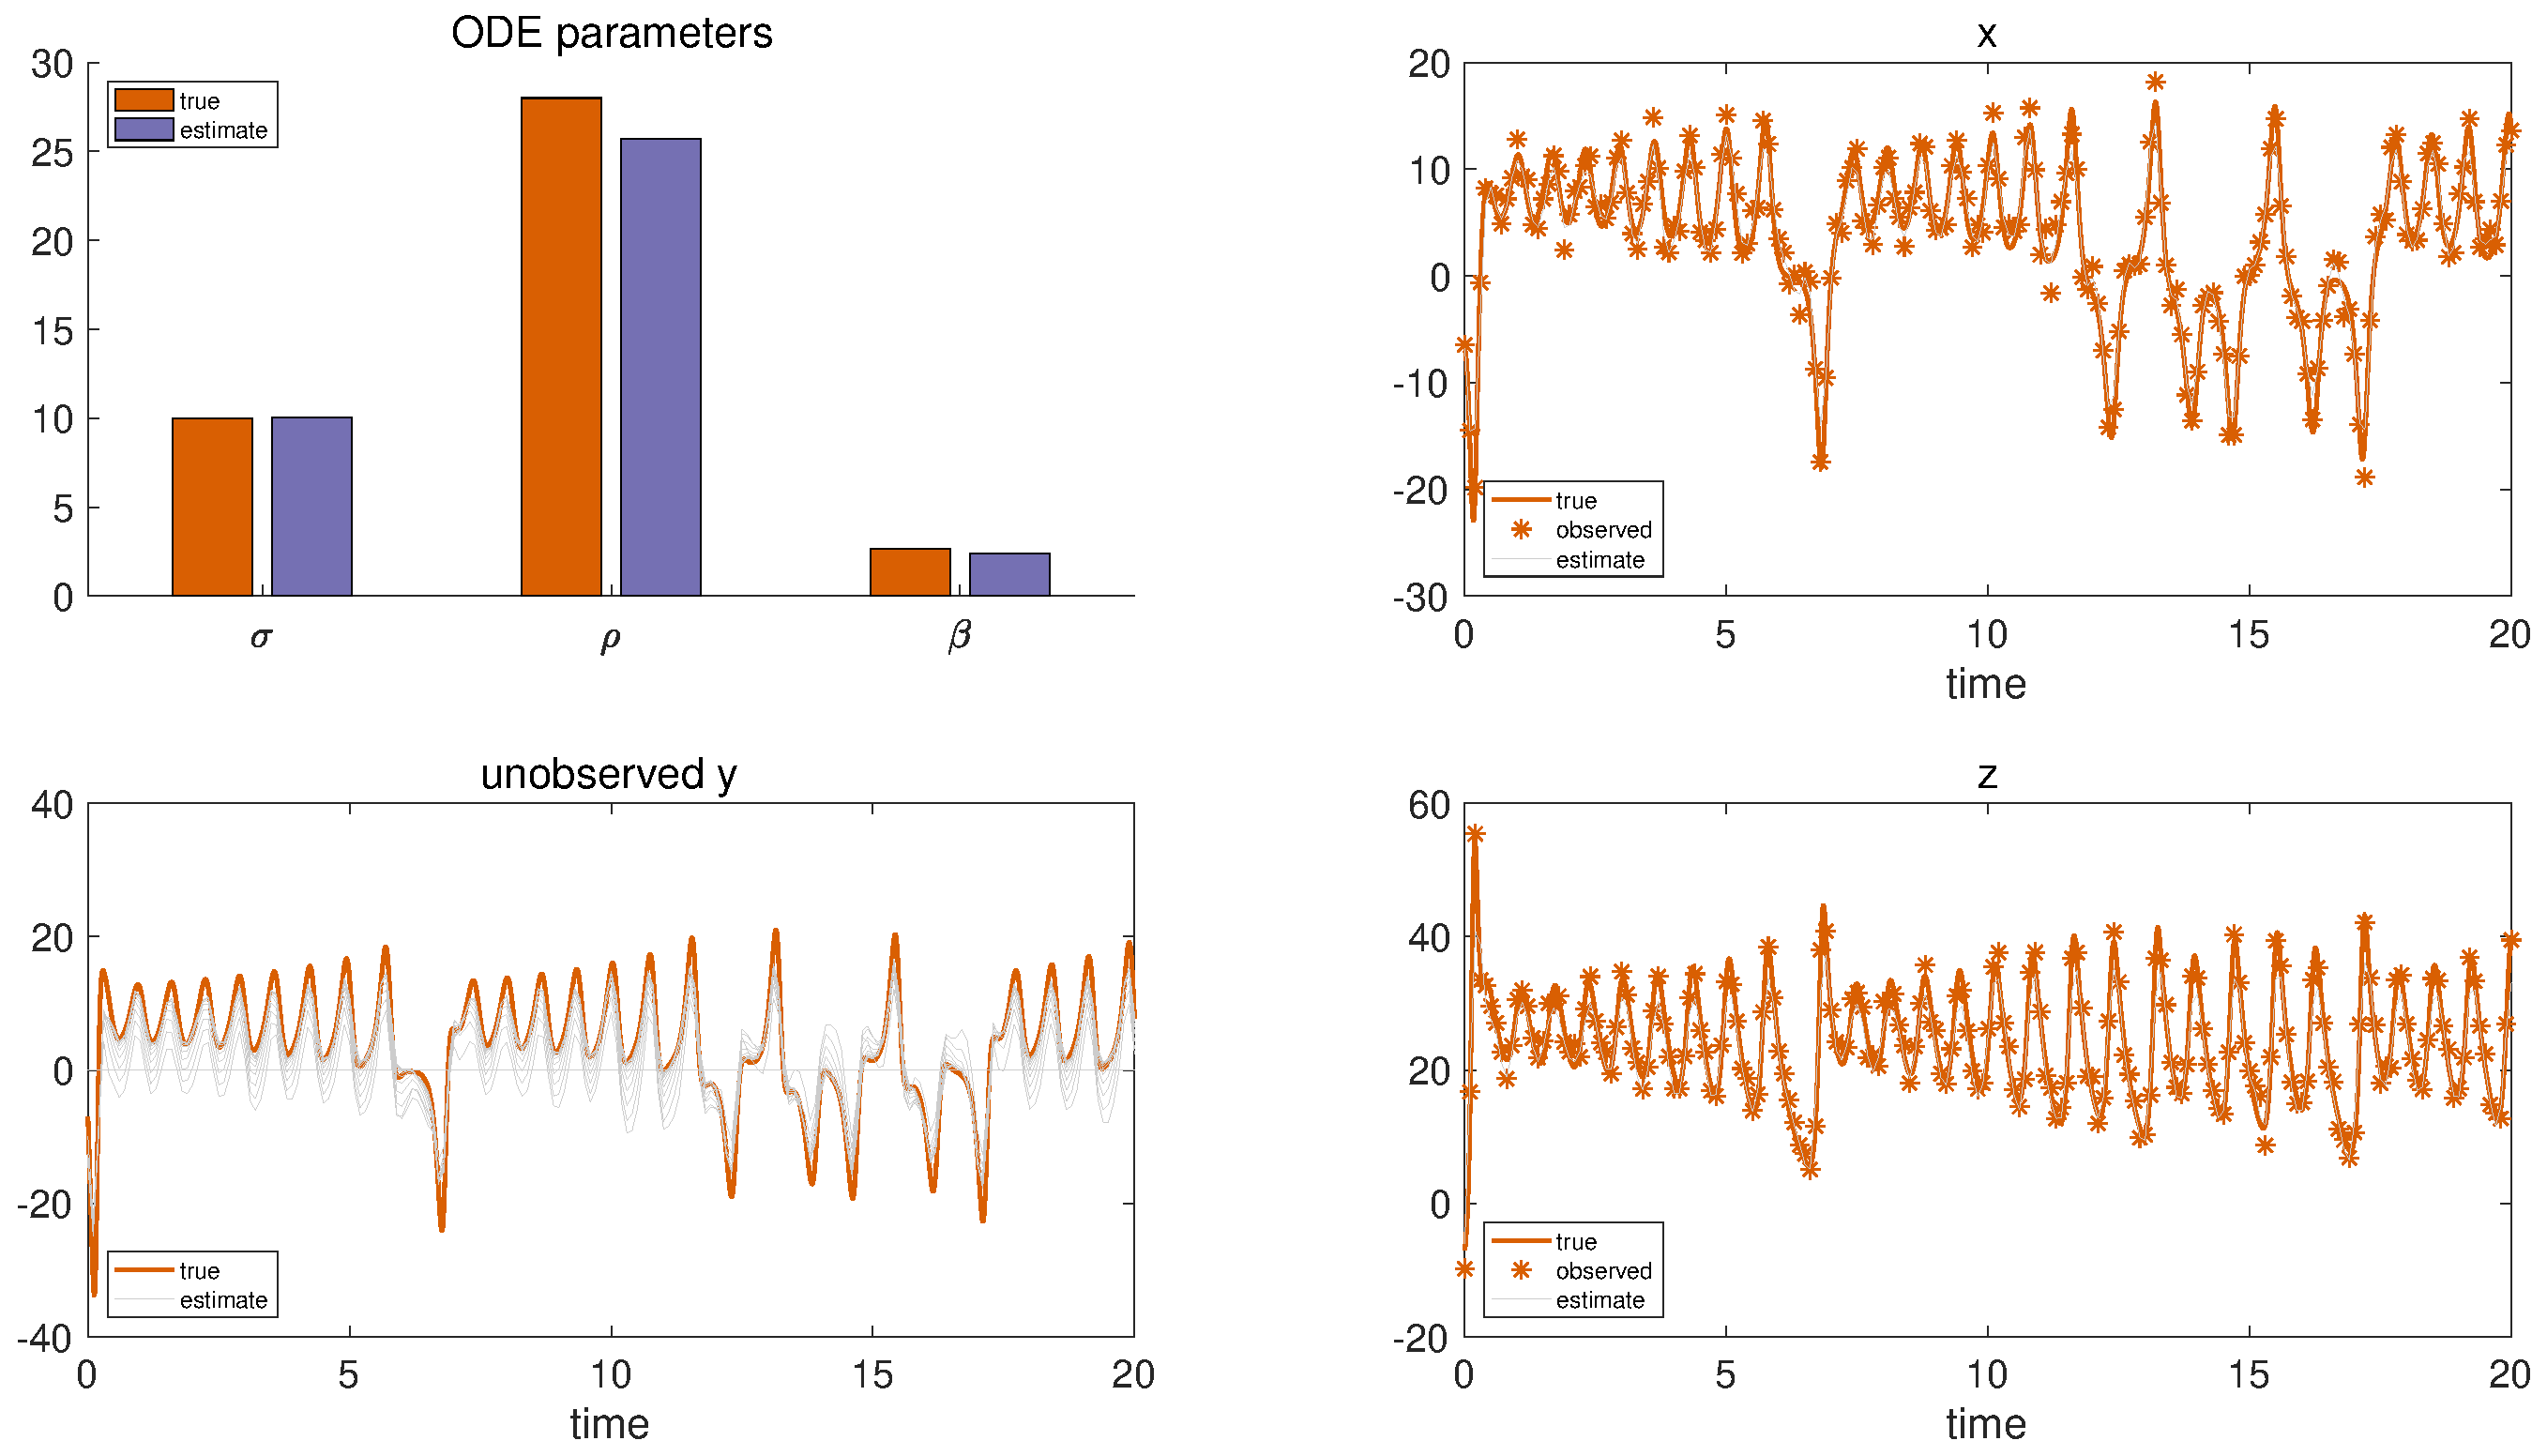
\includegraphics [width=5in]{Lorenz_attractor_4_32.eps}

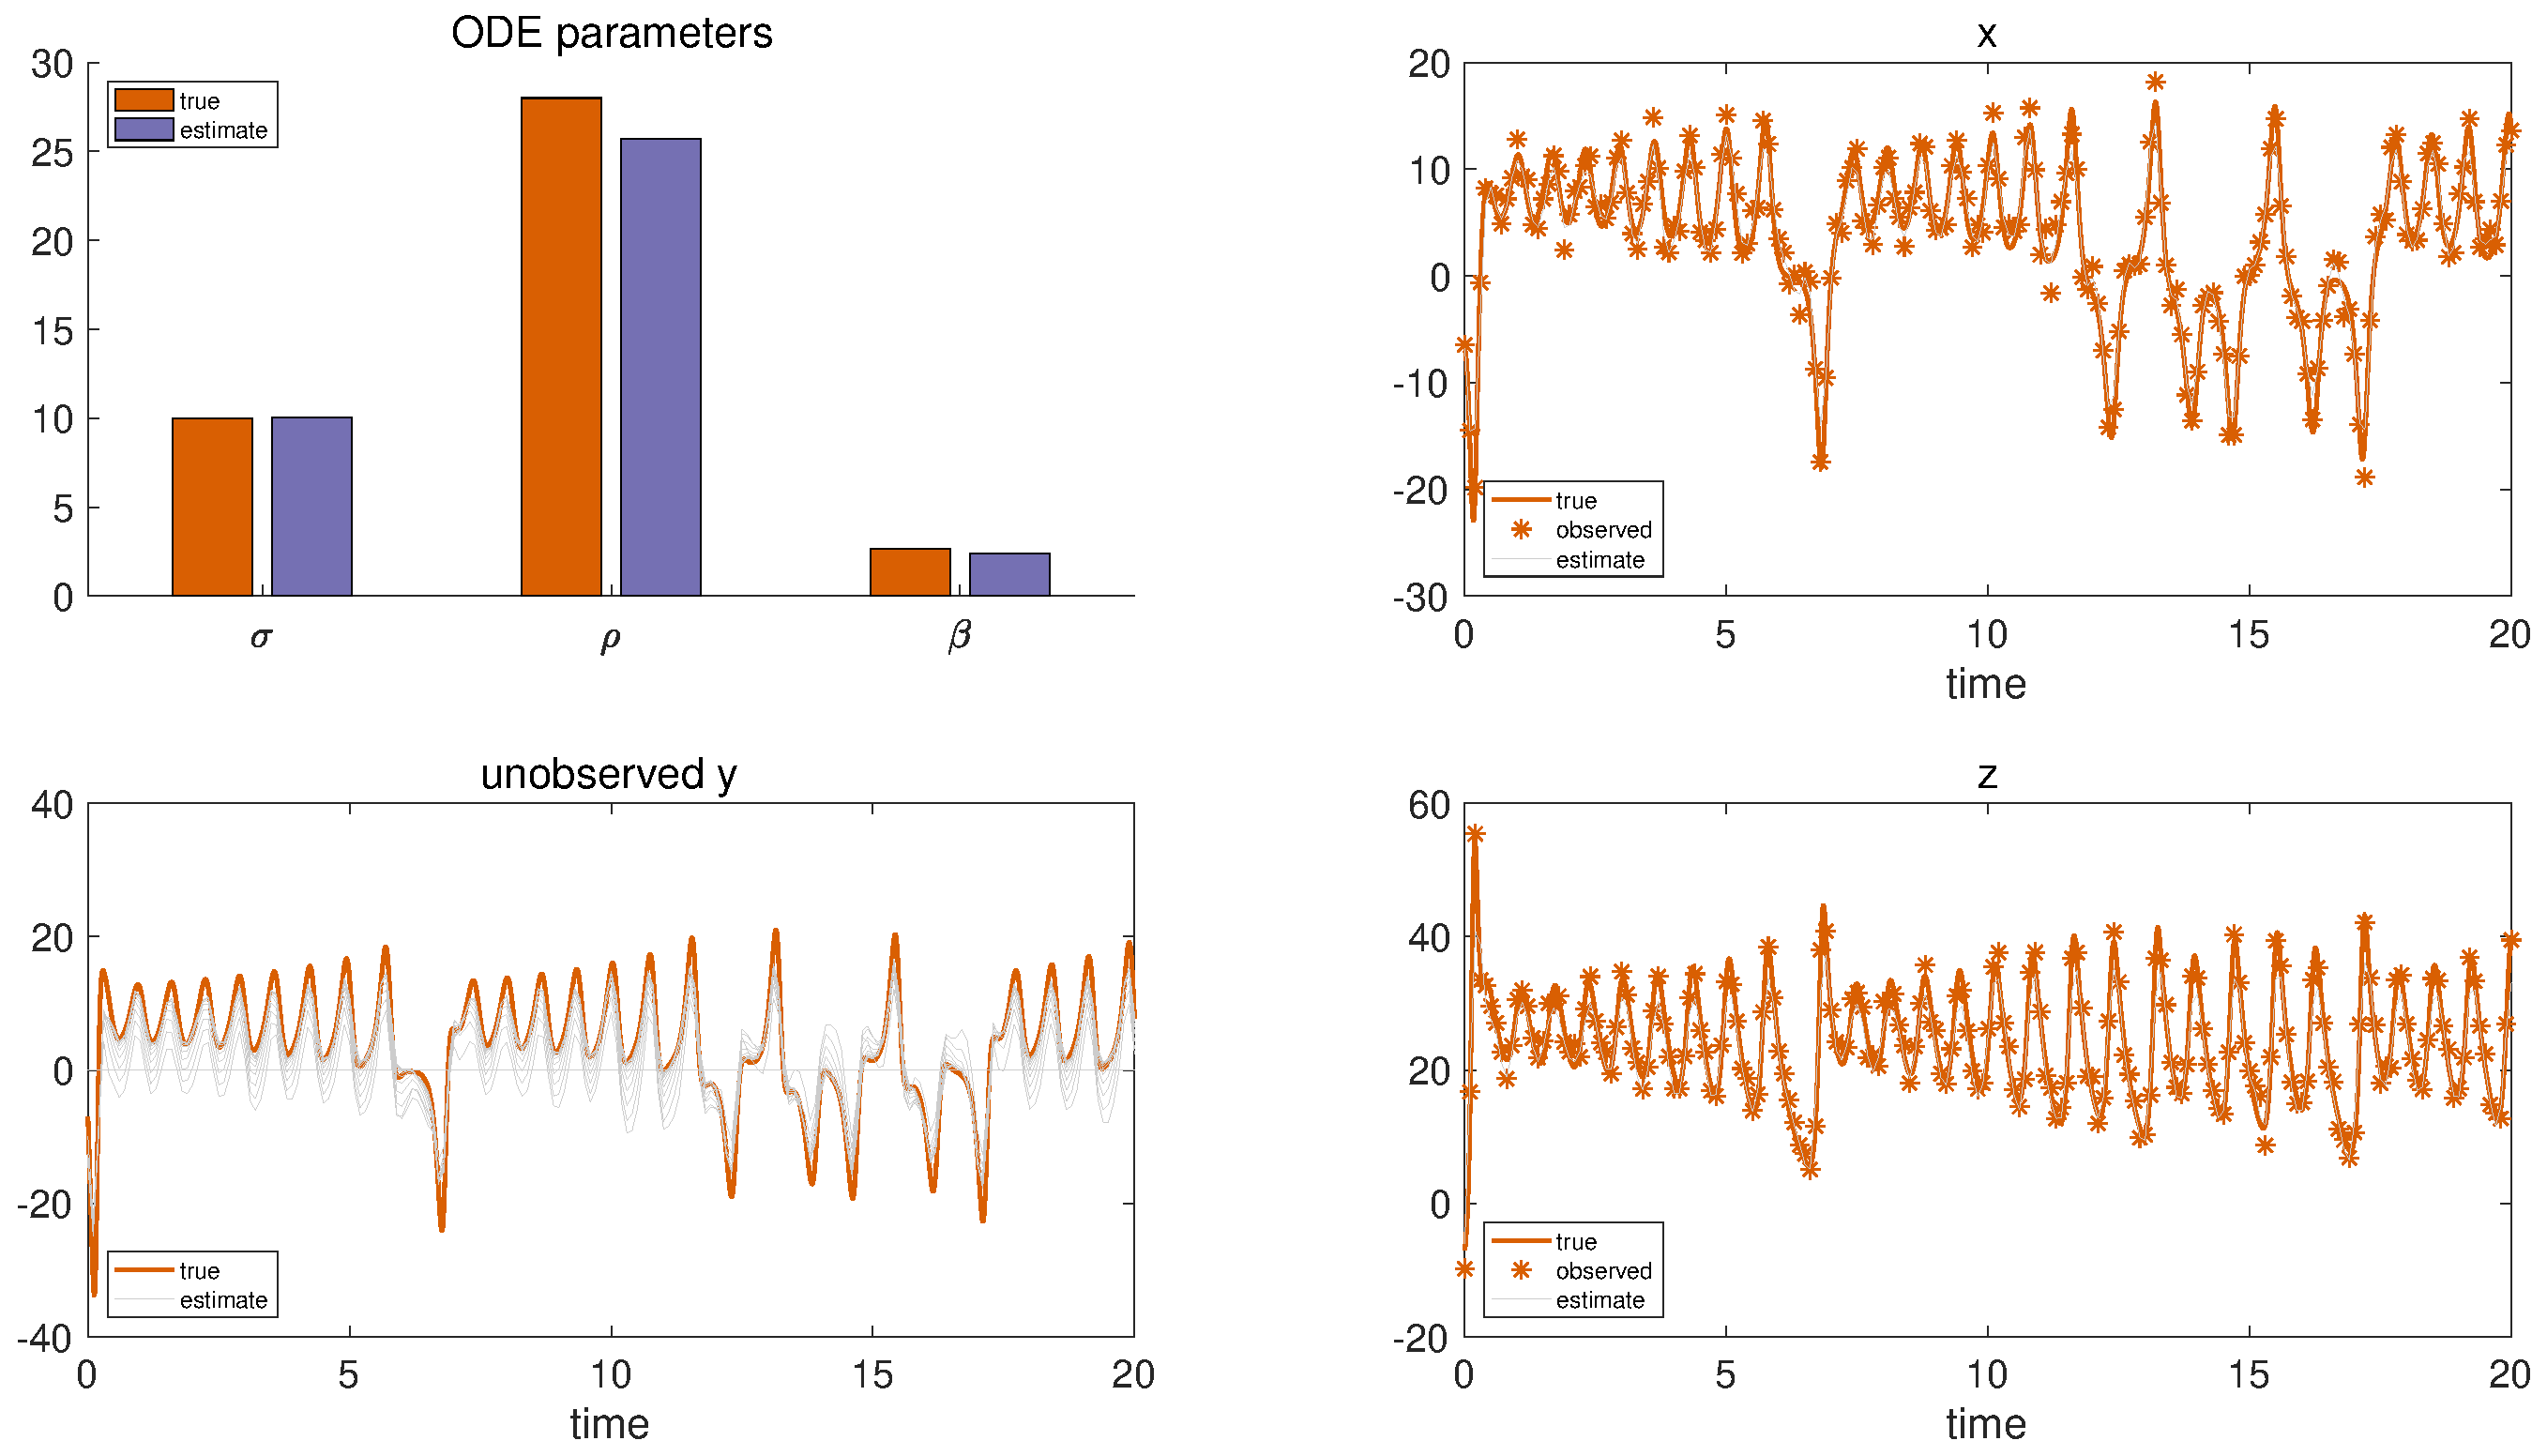
\includegraphics [width=5in]{Lorenz_attractor_4_33.eps}

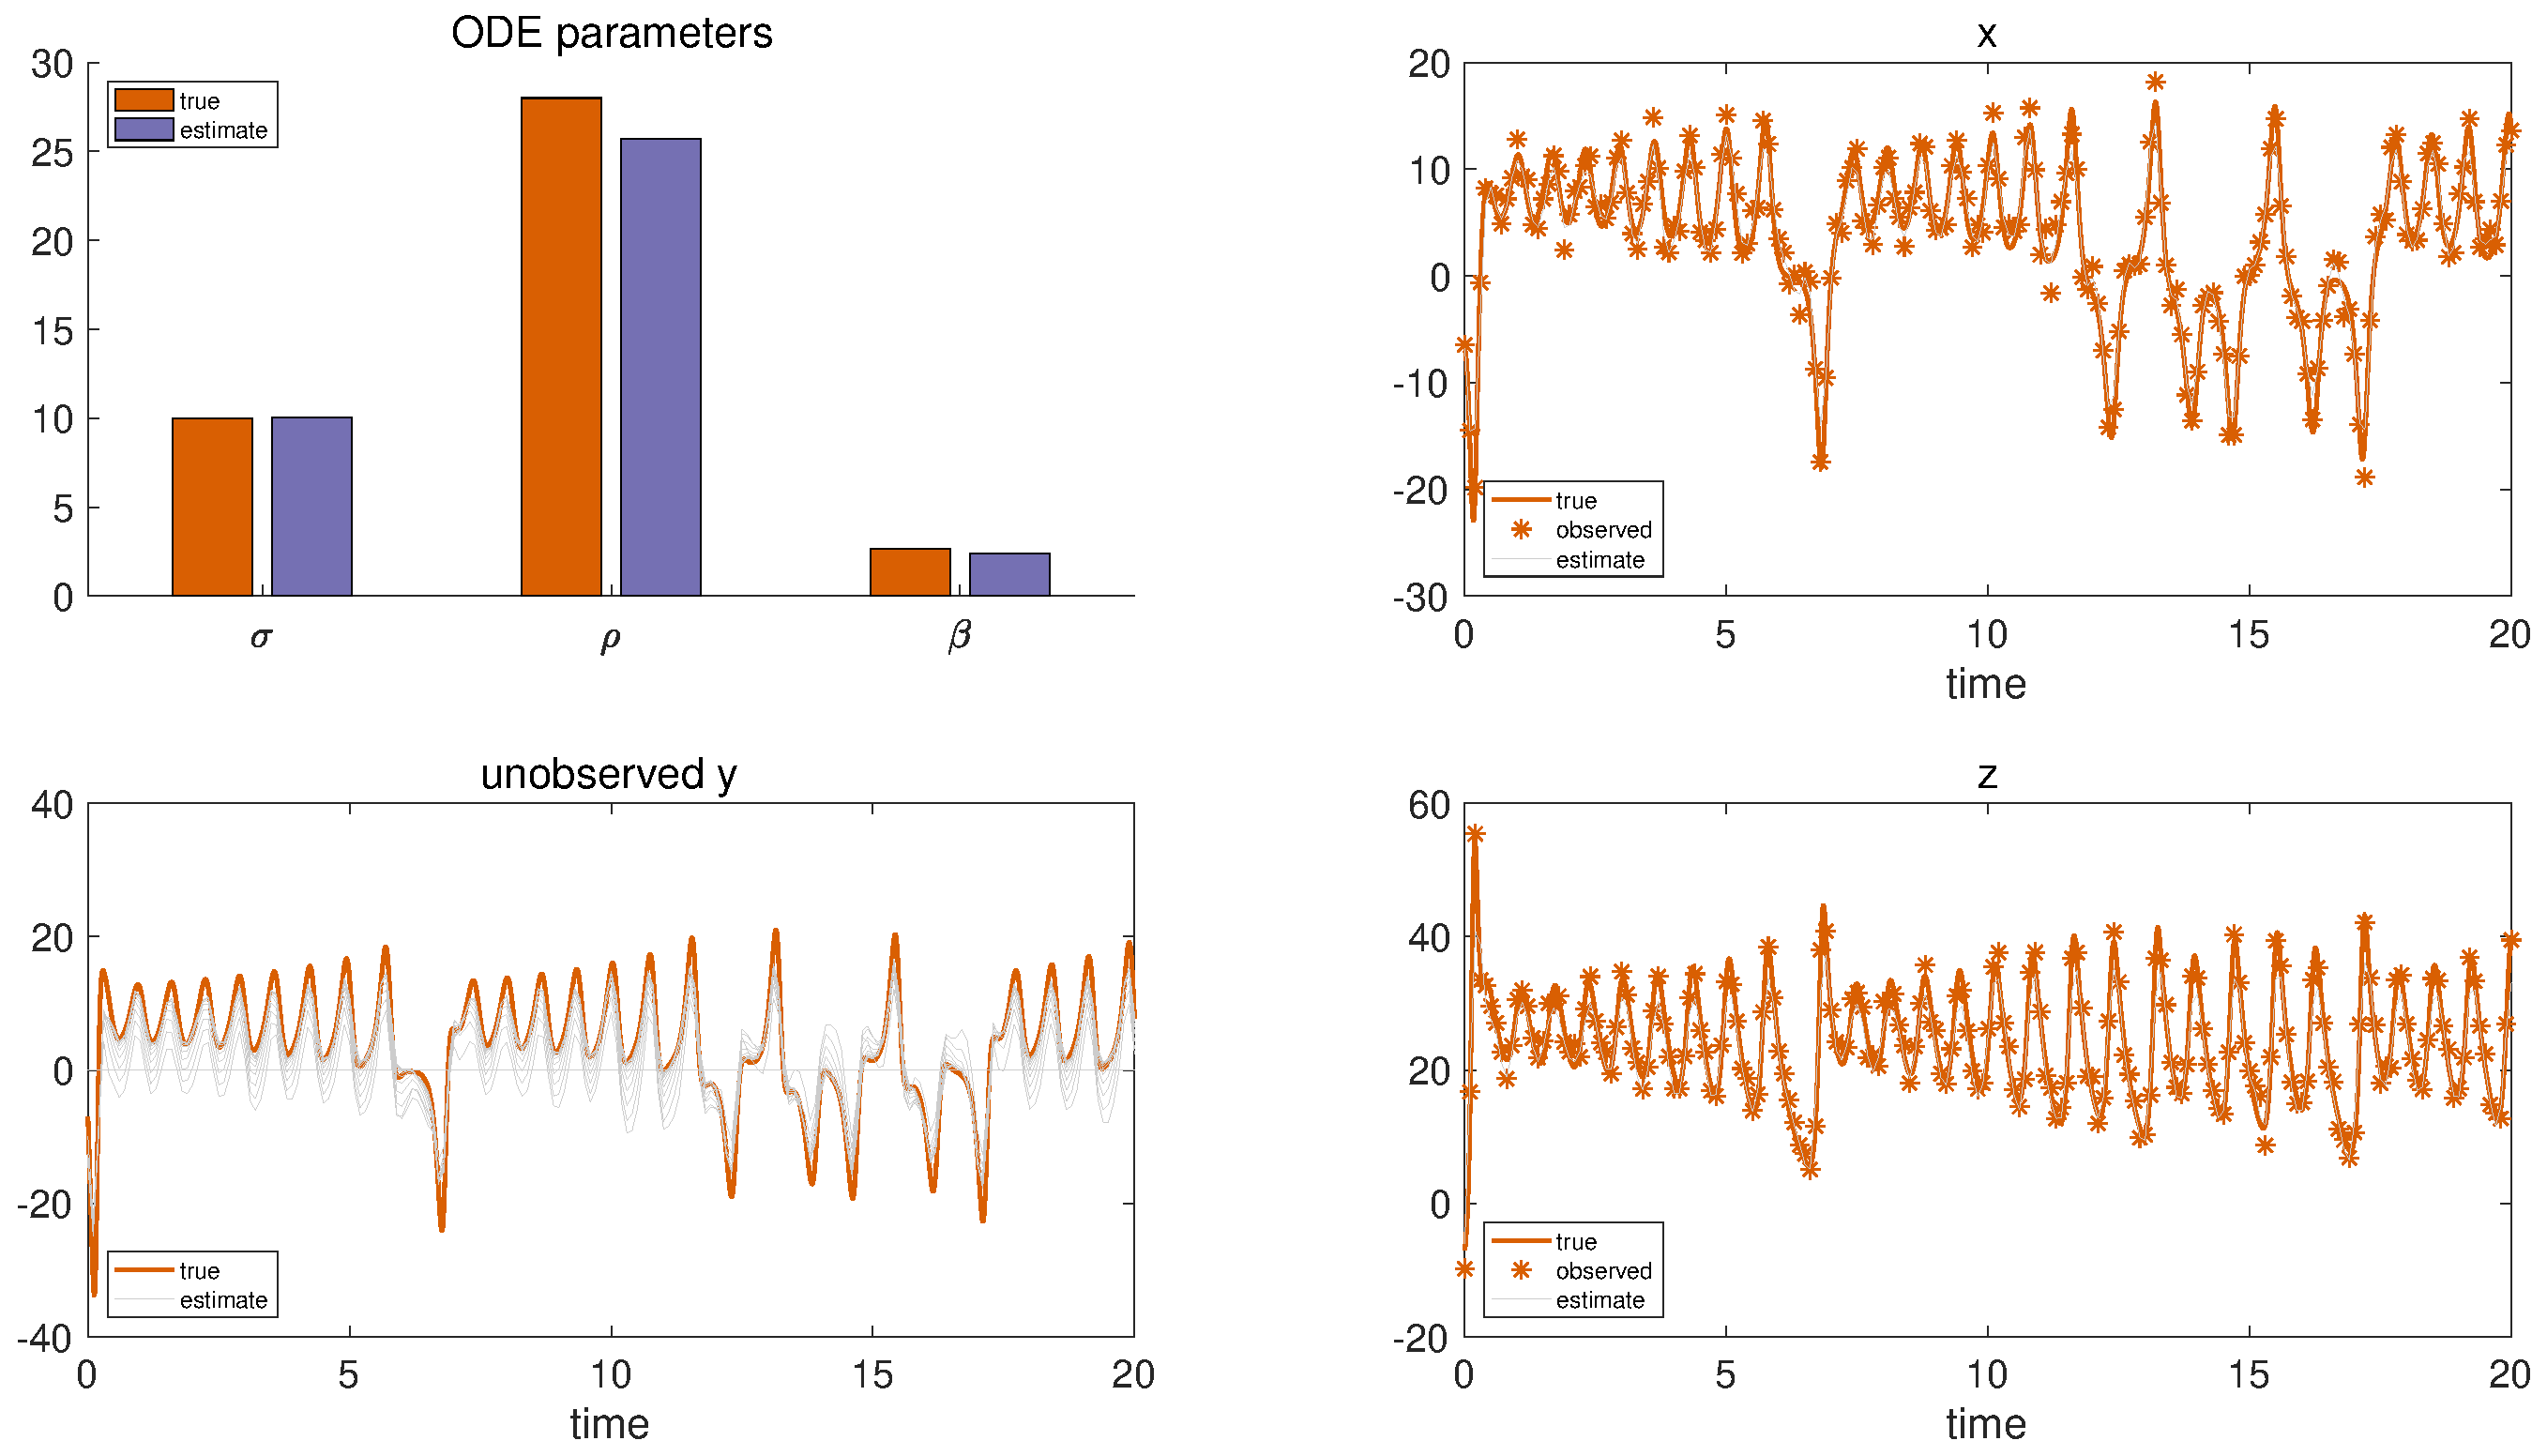
\includegraphics [width=5in]{Lorenz_attractor_4_34.eps}

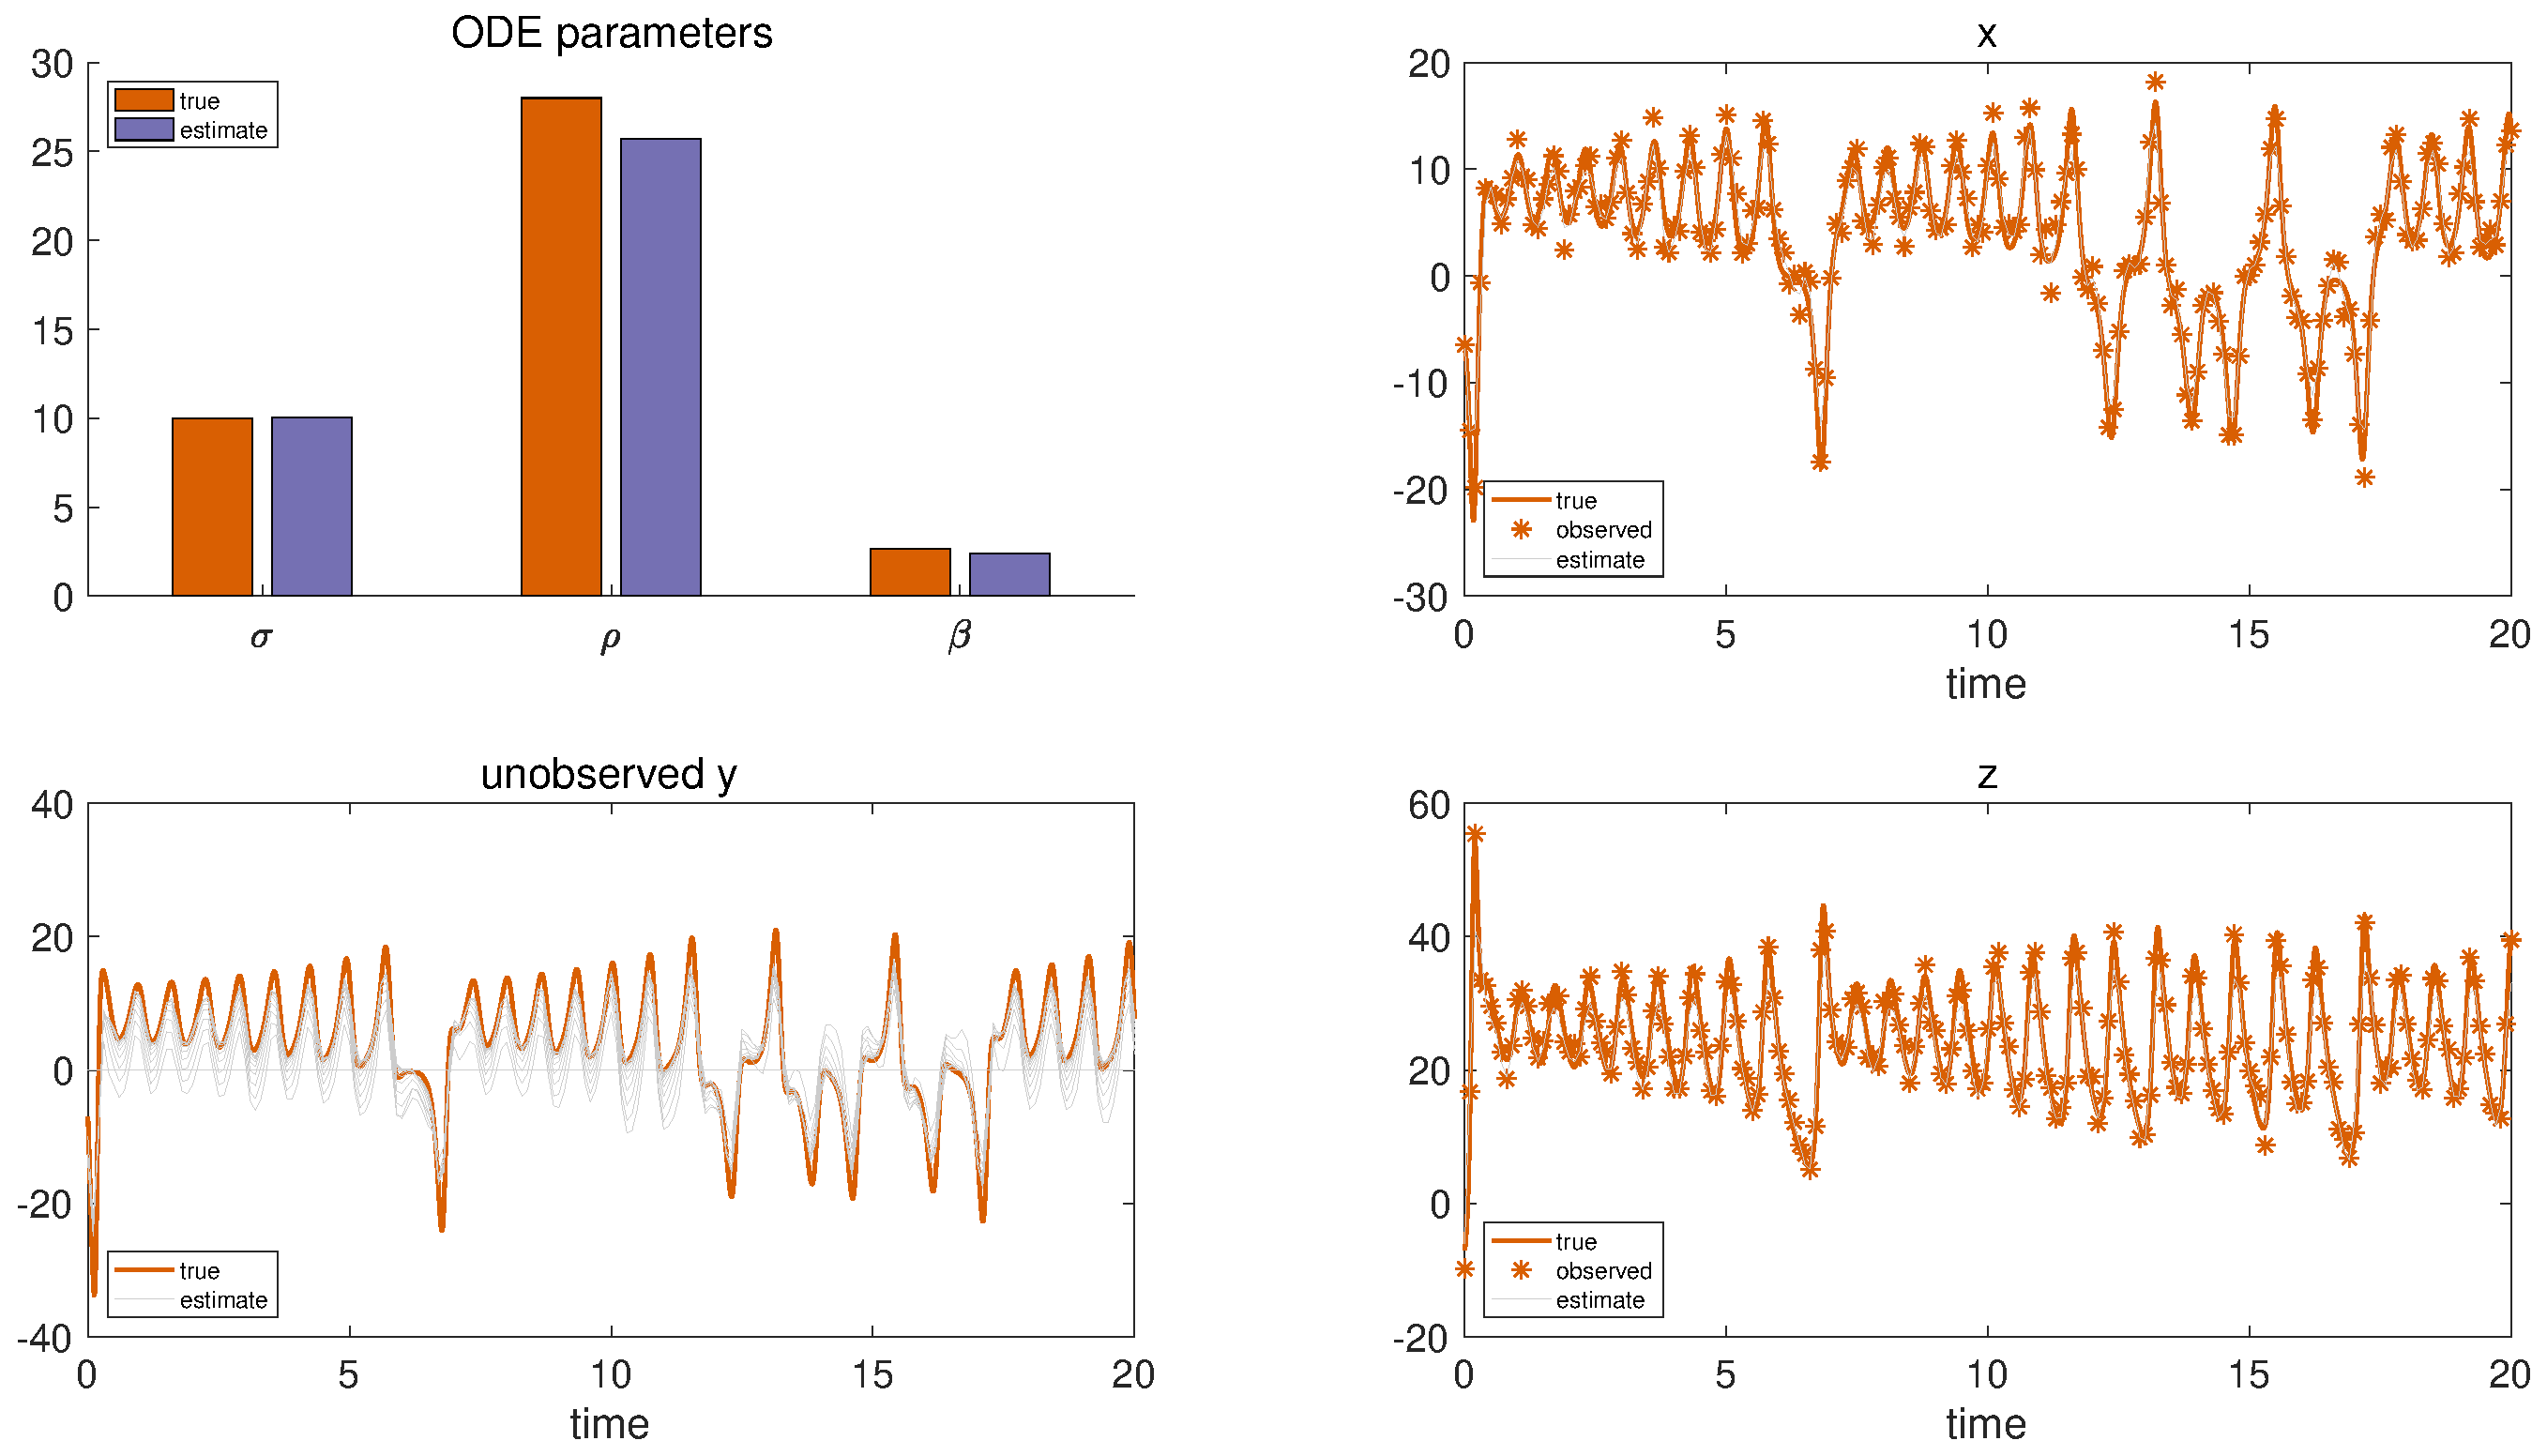
\includegraphics [width=5in]{Lorenz_attractor_4_35.eps}

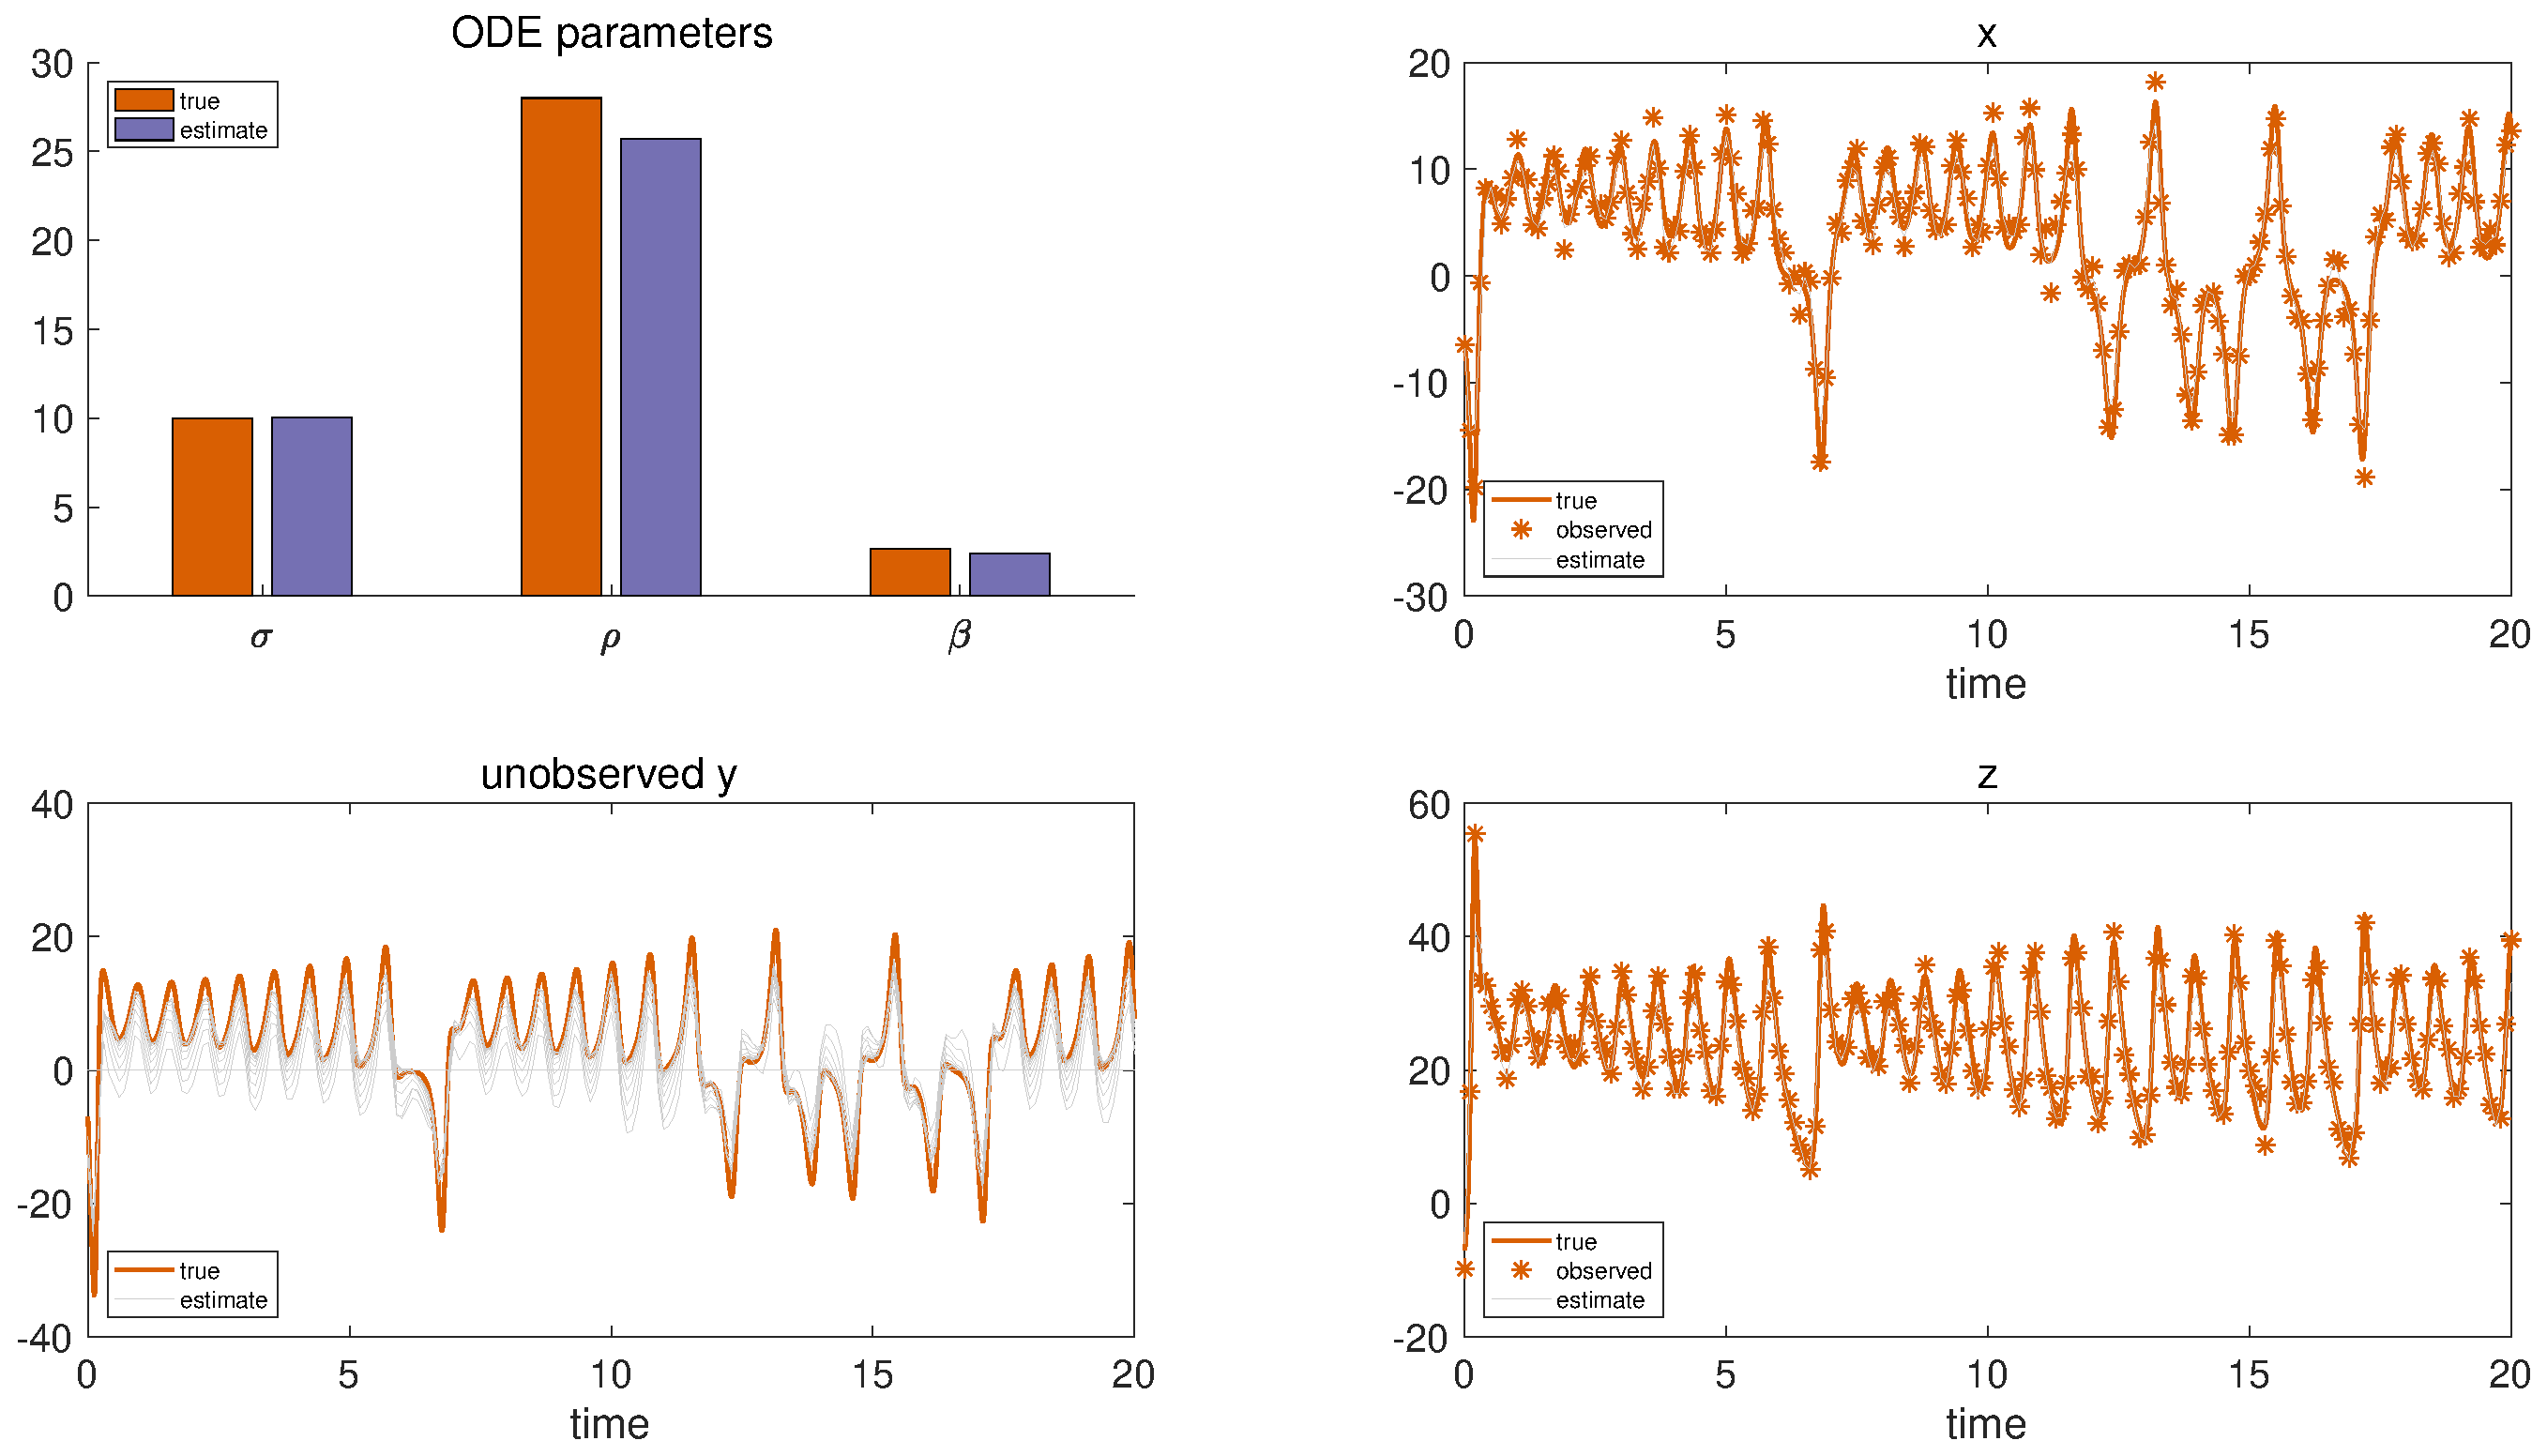
\includegraphics [width=5in]{Lorenz_attractor_4_36.eps}

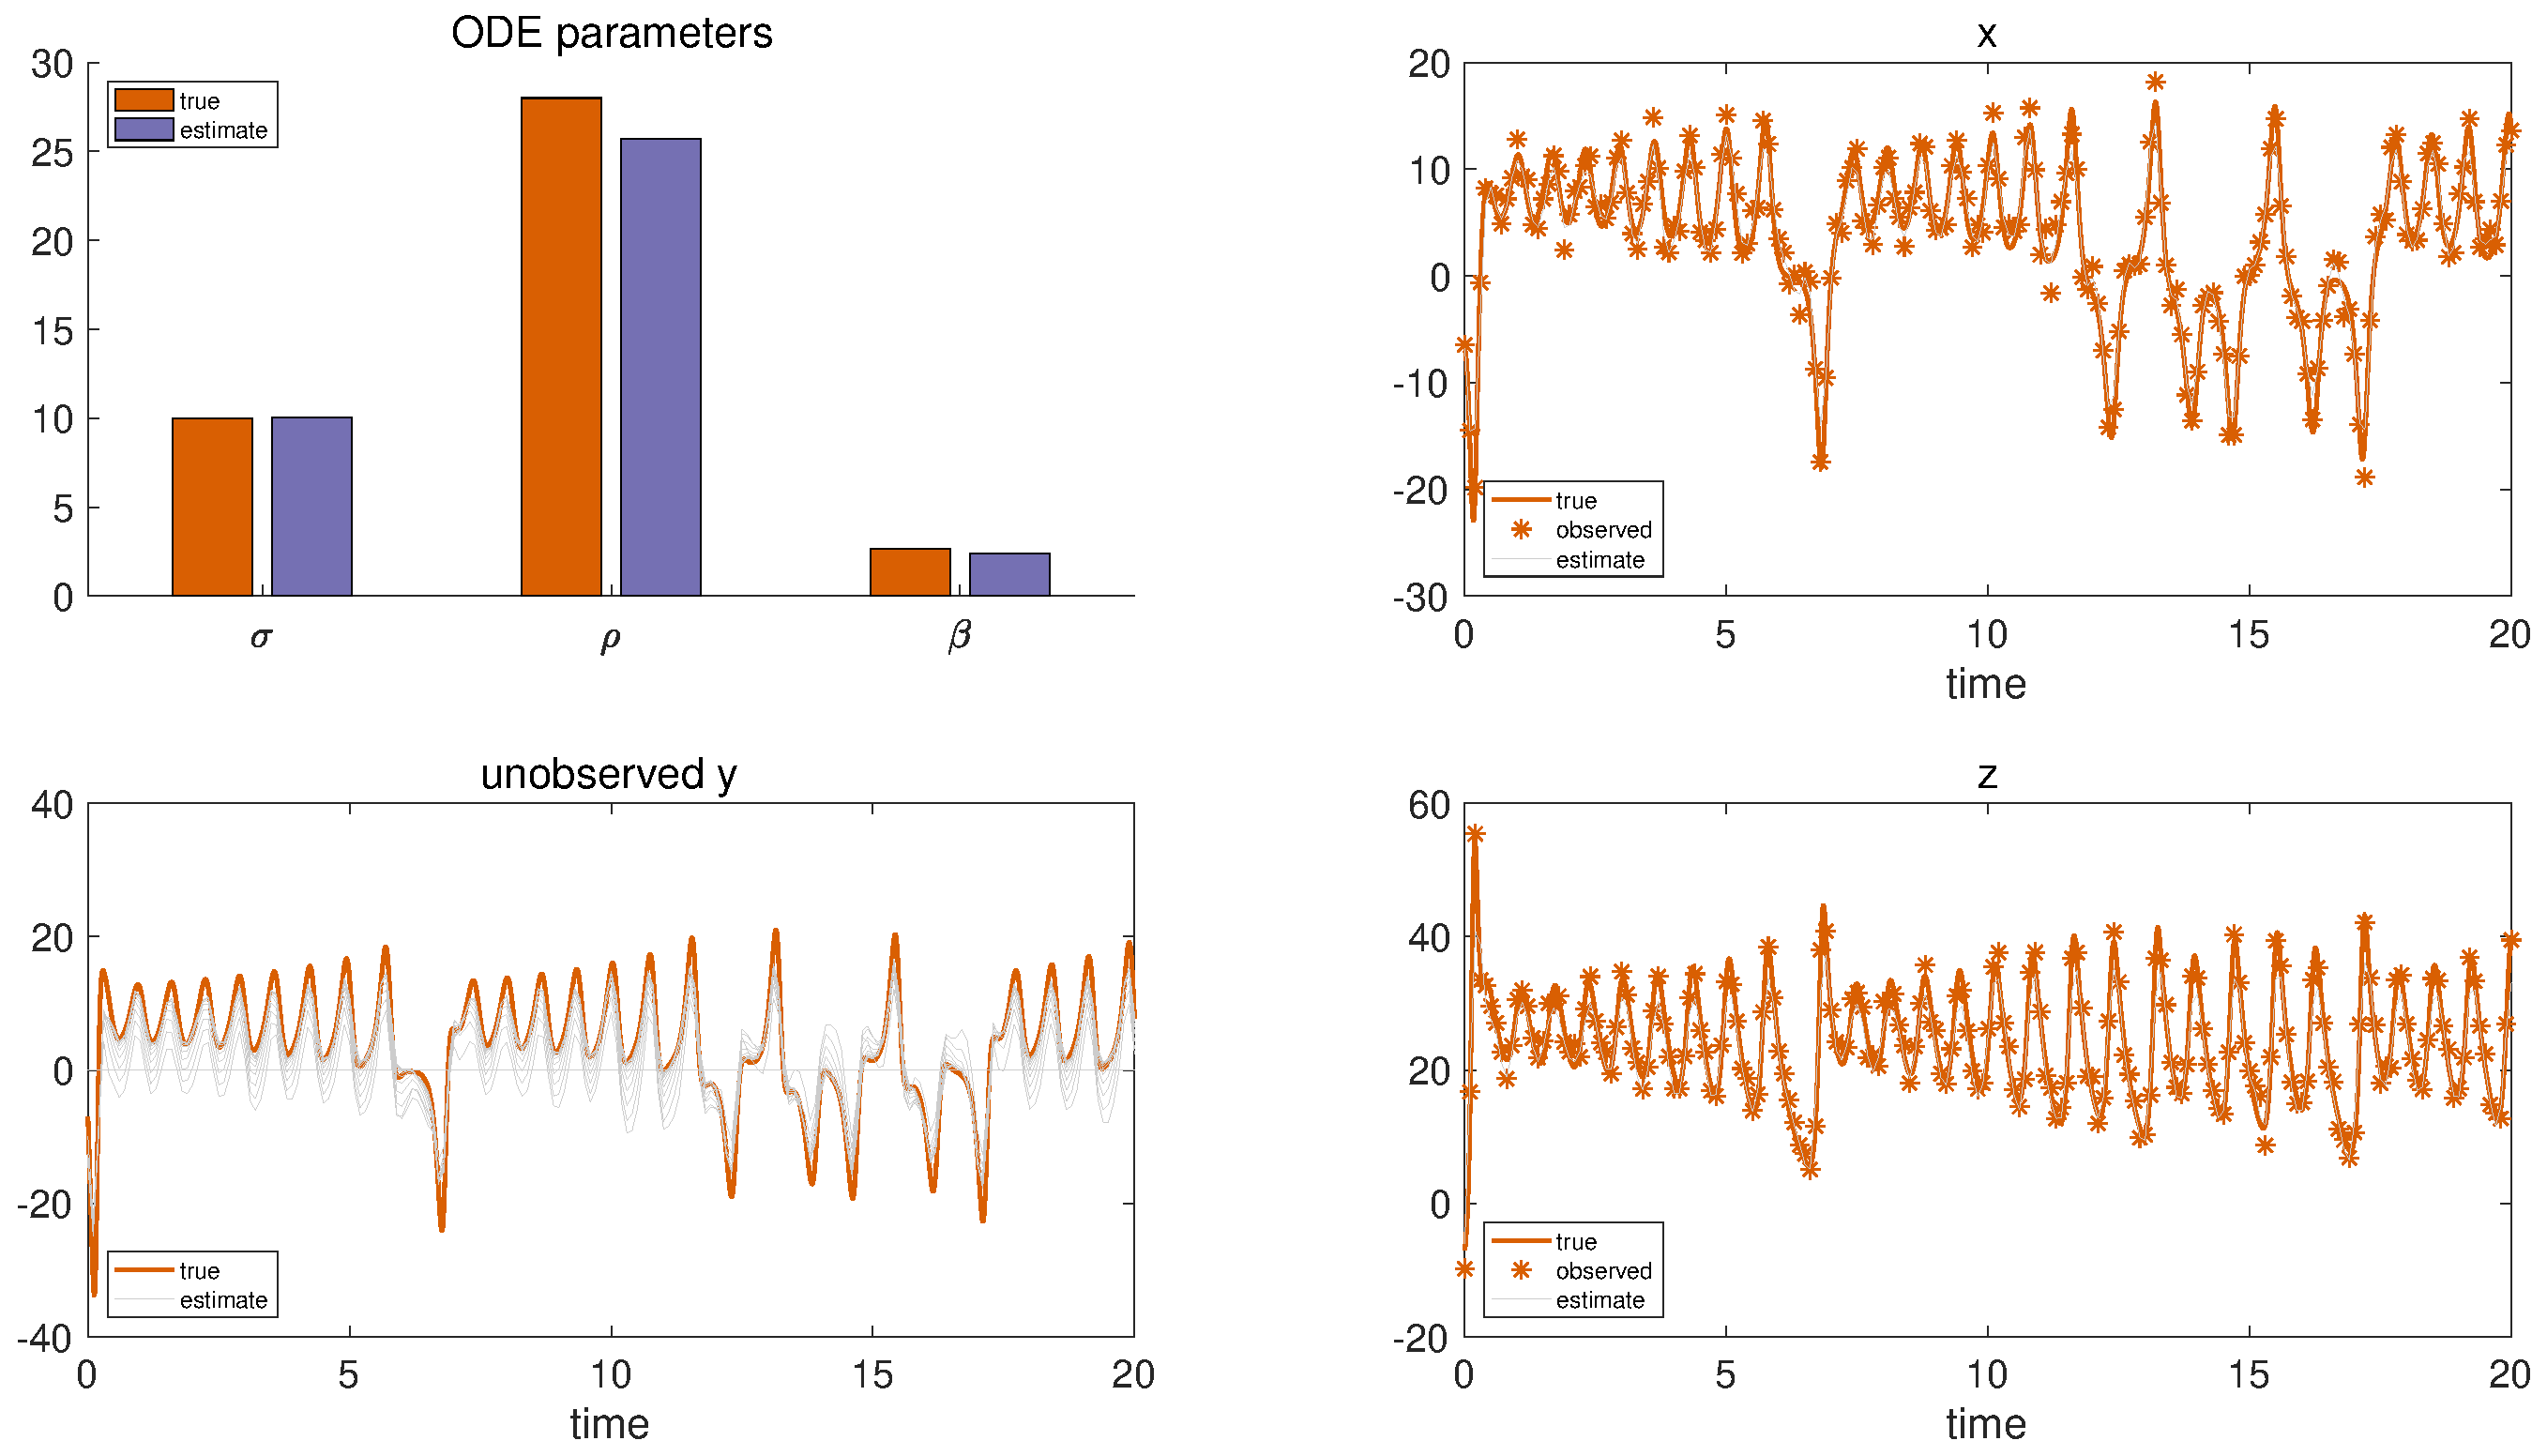
\includegraphics [width=5in]{Lorenz_attractor_4_37.eps}

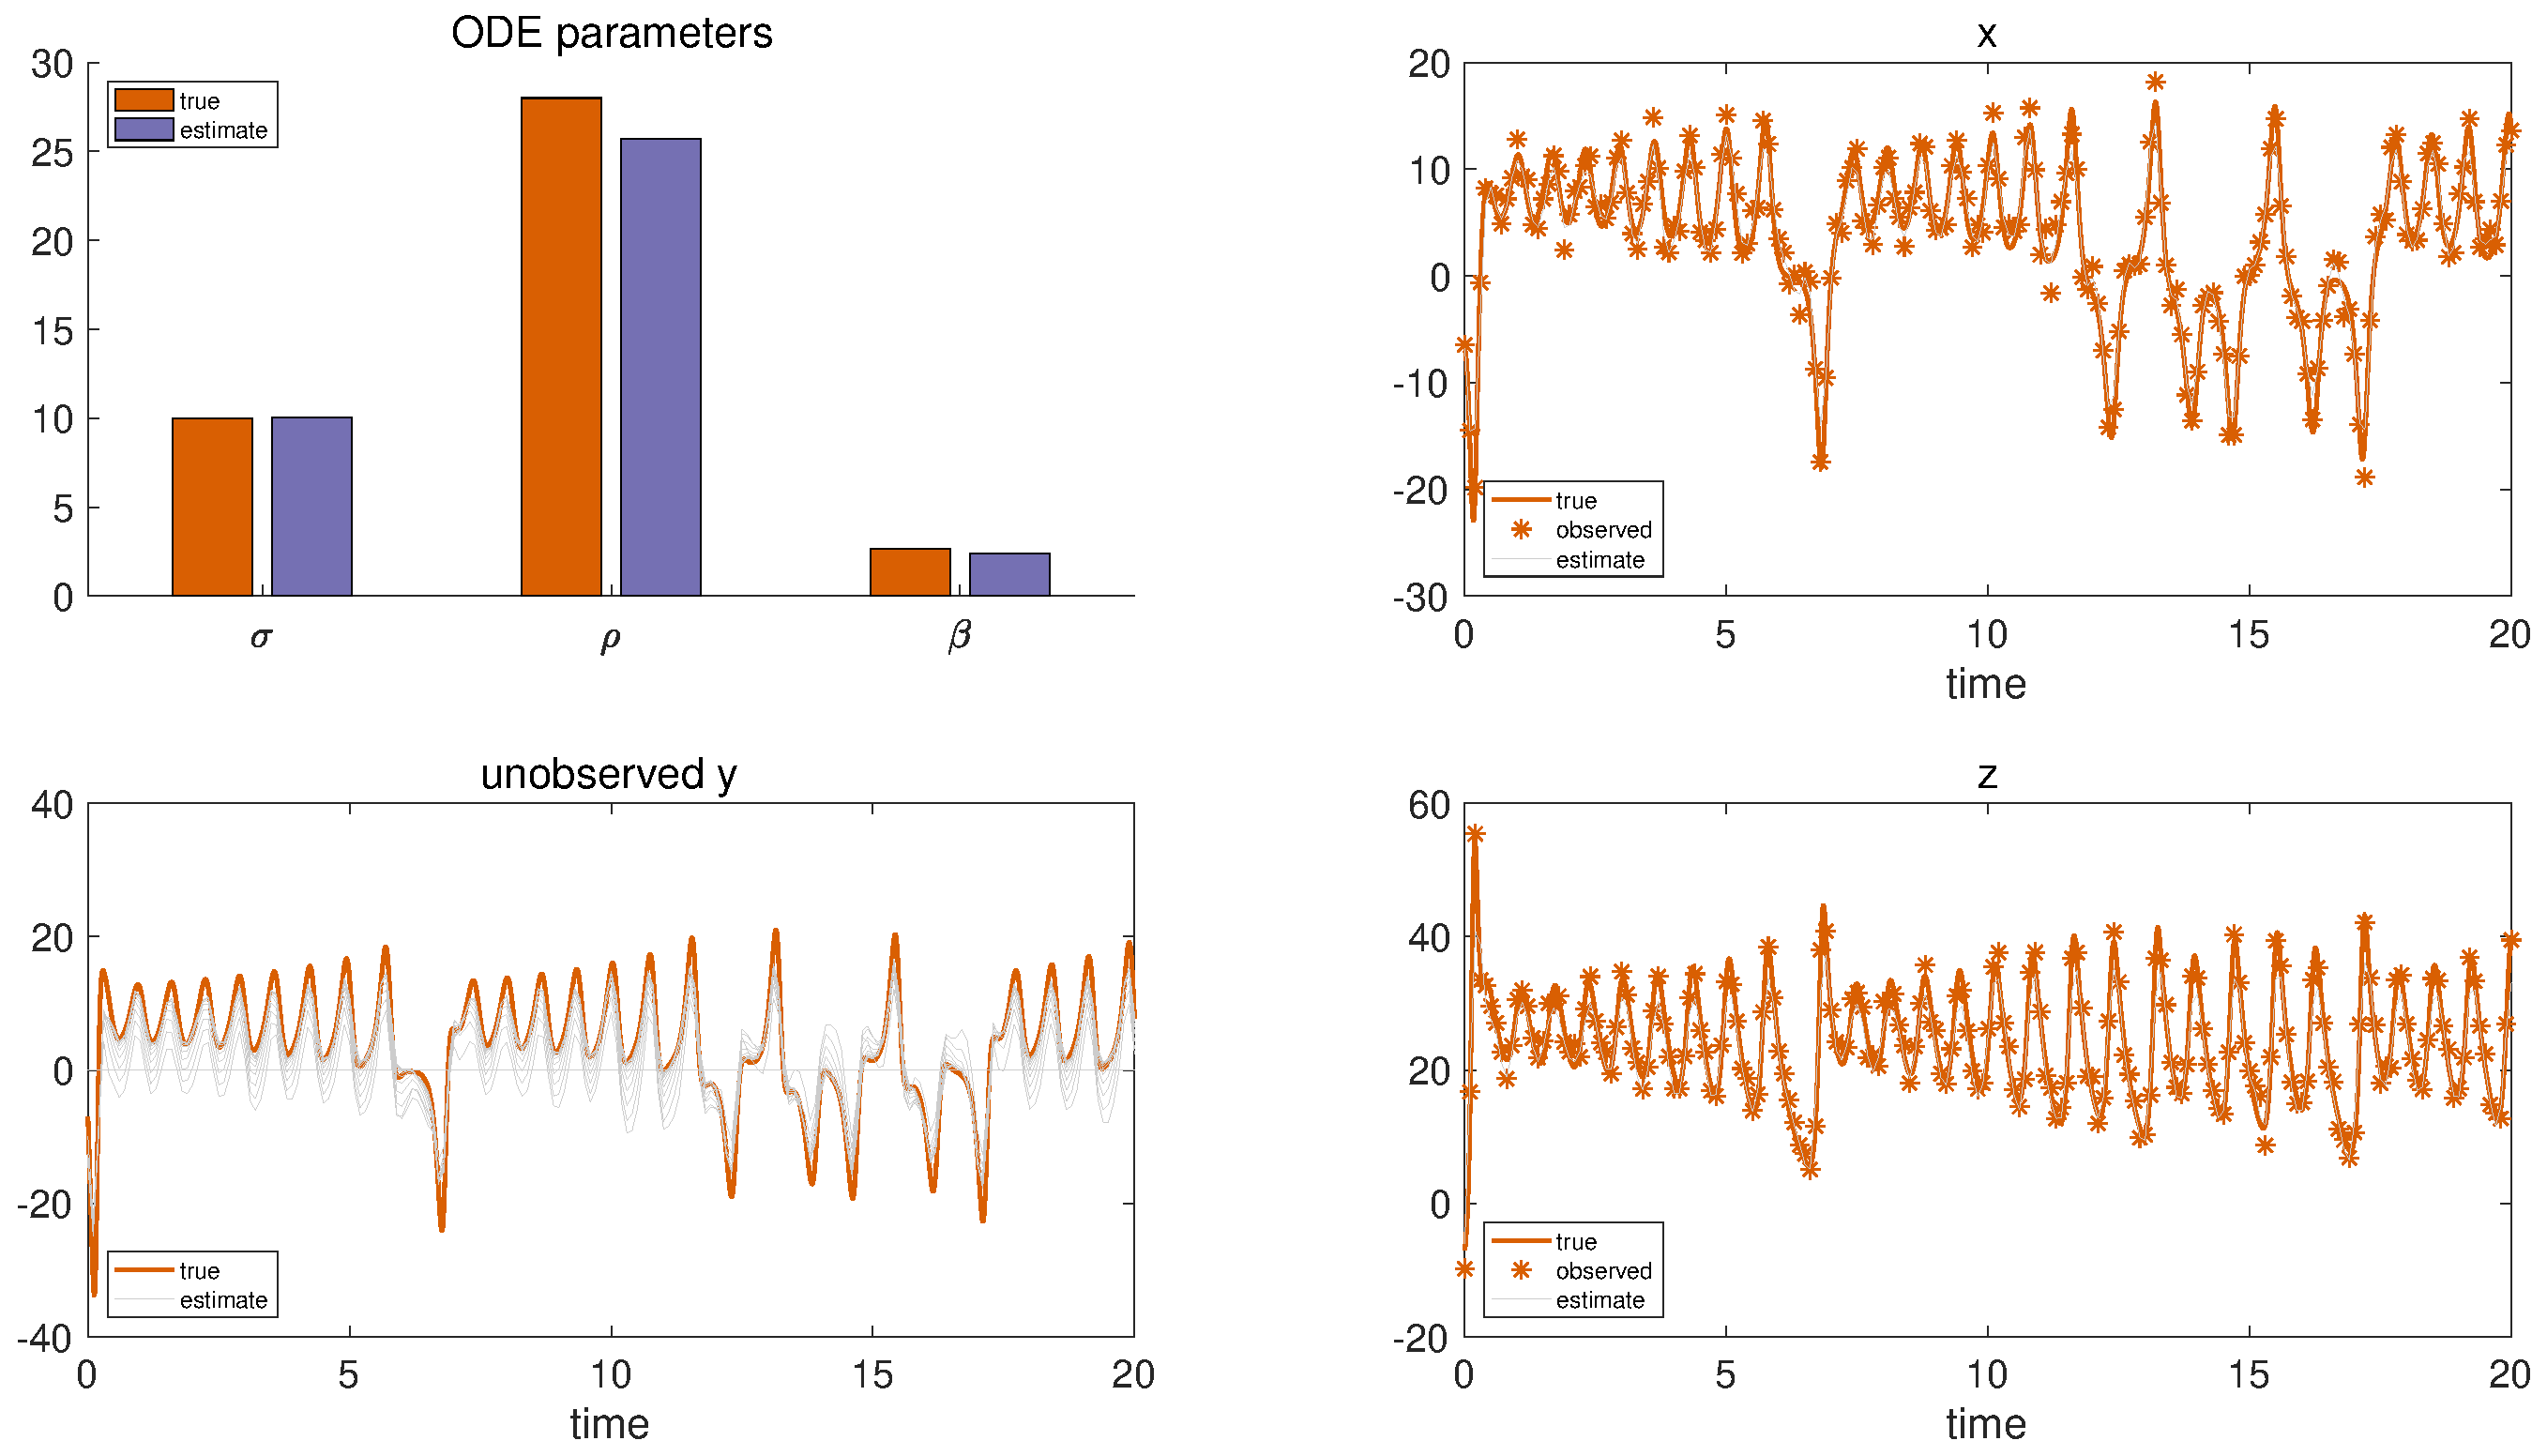
\includegraphics [width=5in]{Lorenz_attractor_4_38.eps}

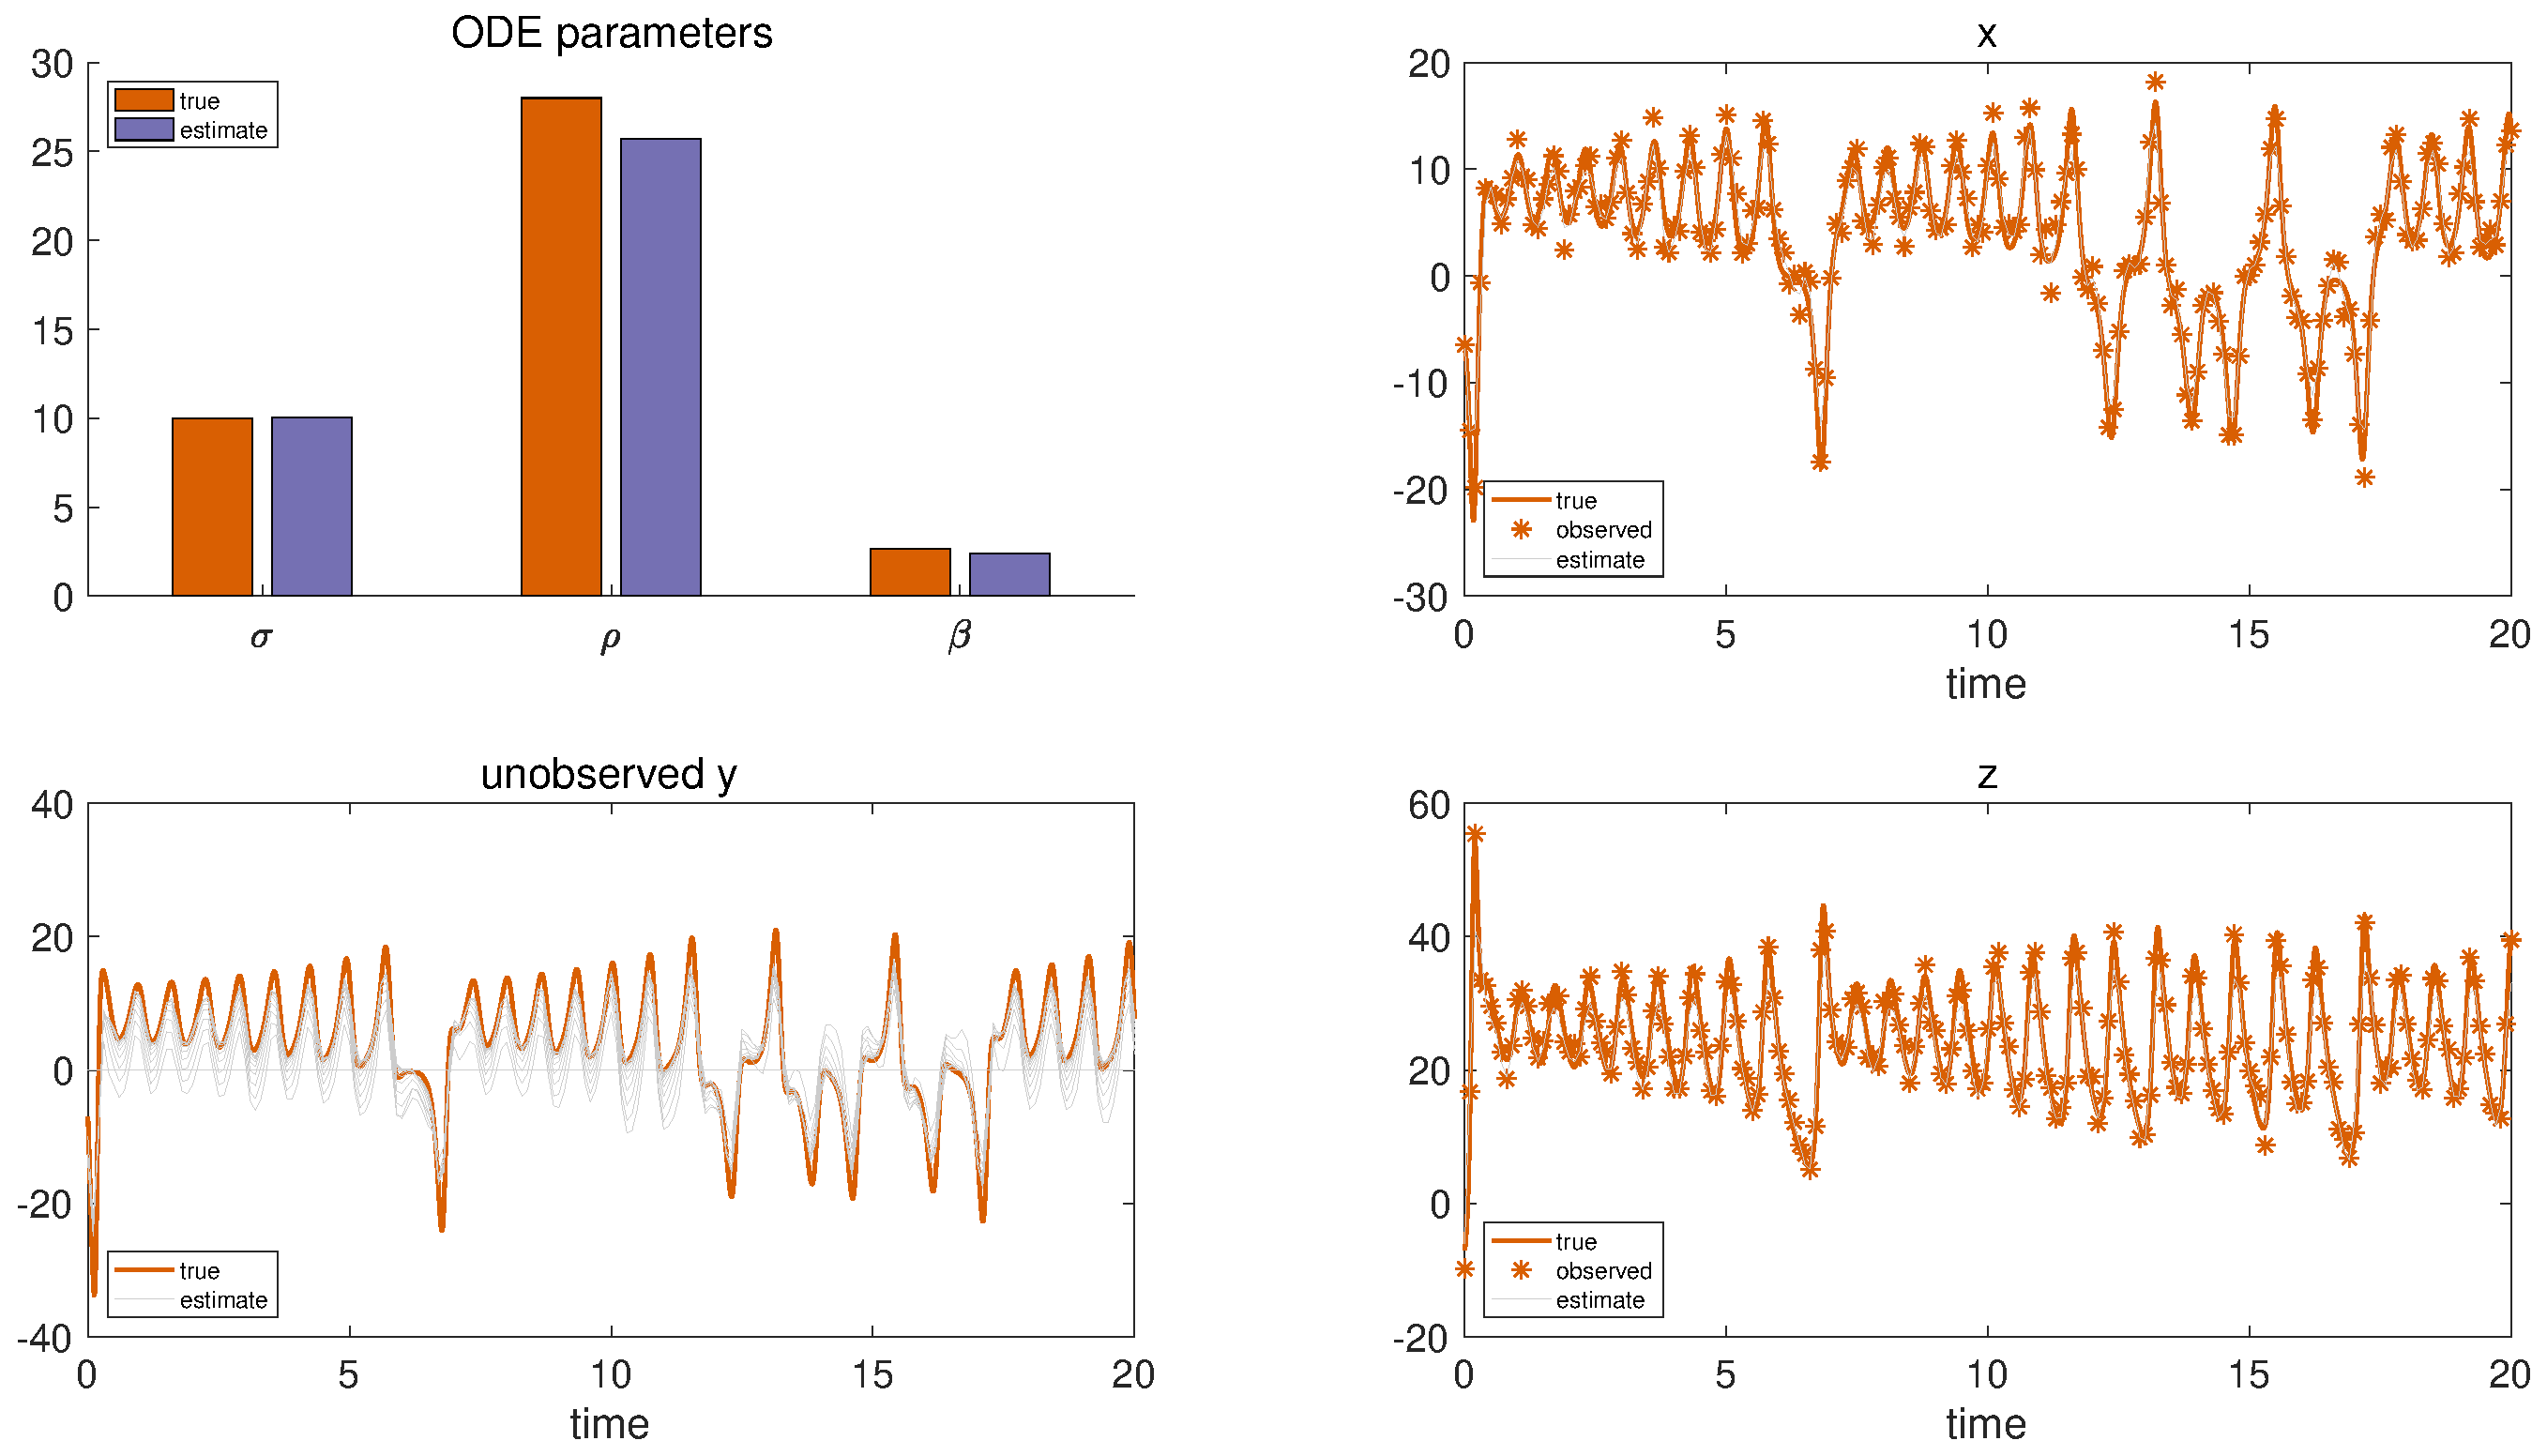
\includegraphics [width=5in]{Lorenz_attractor_4_39.eps}

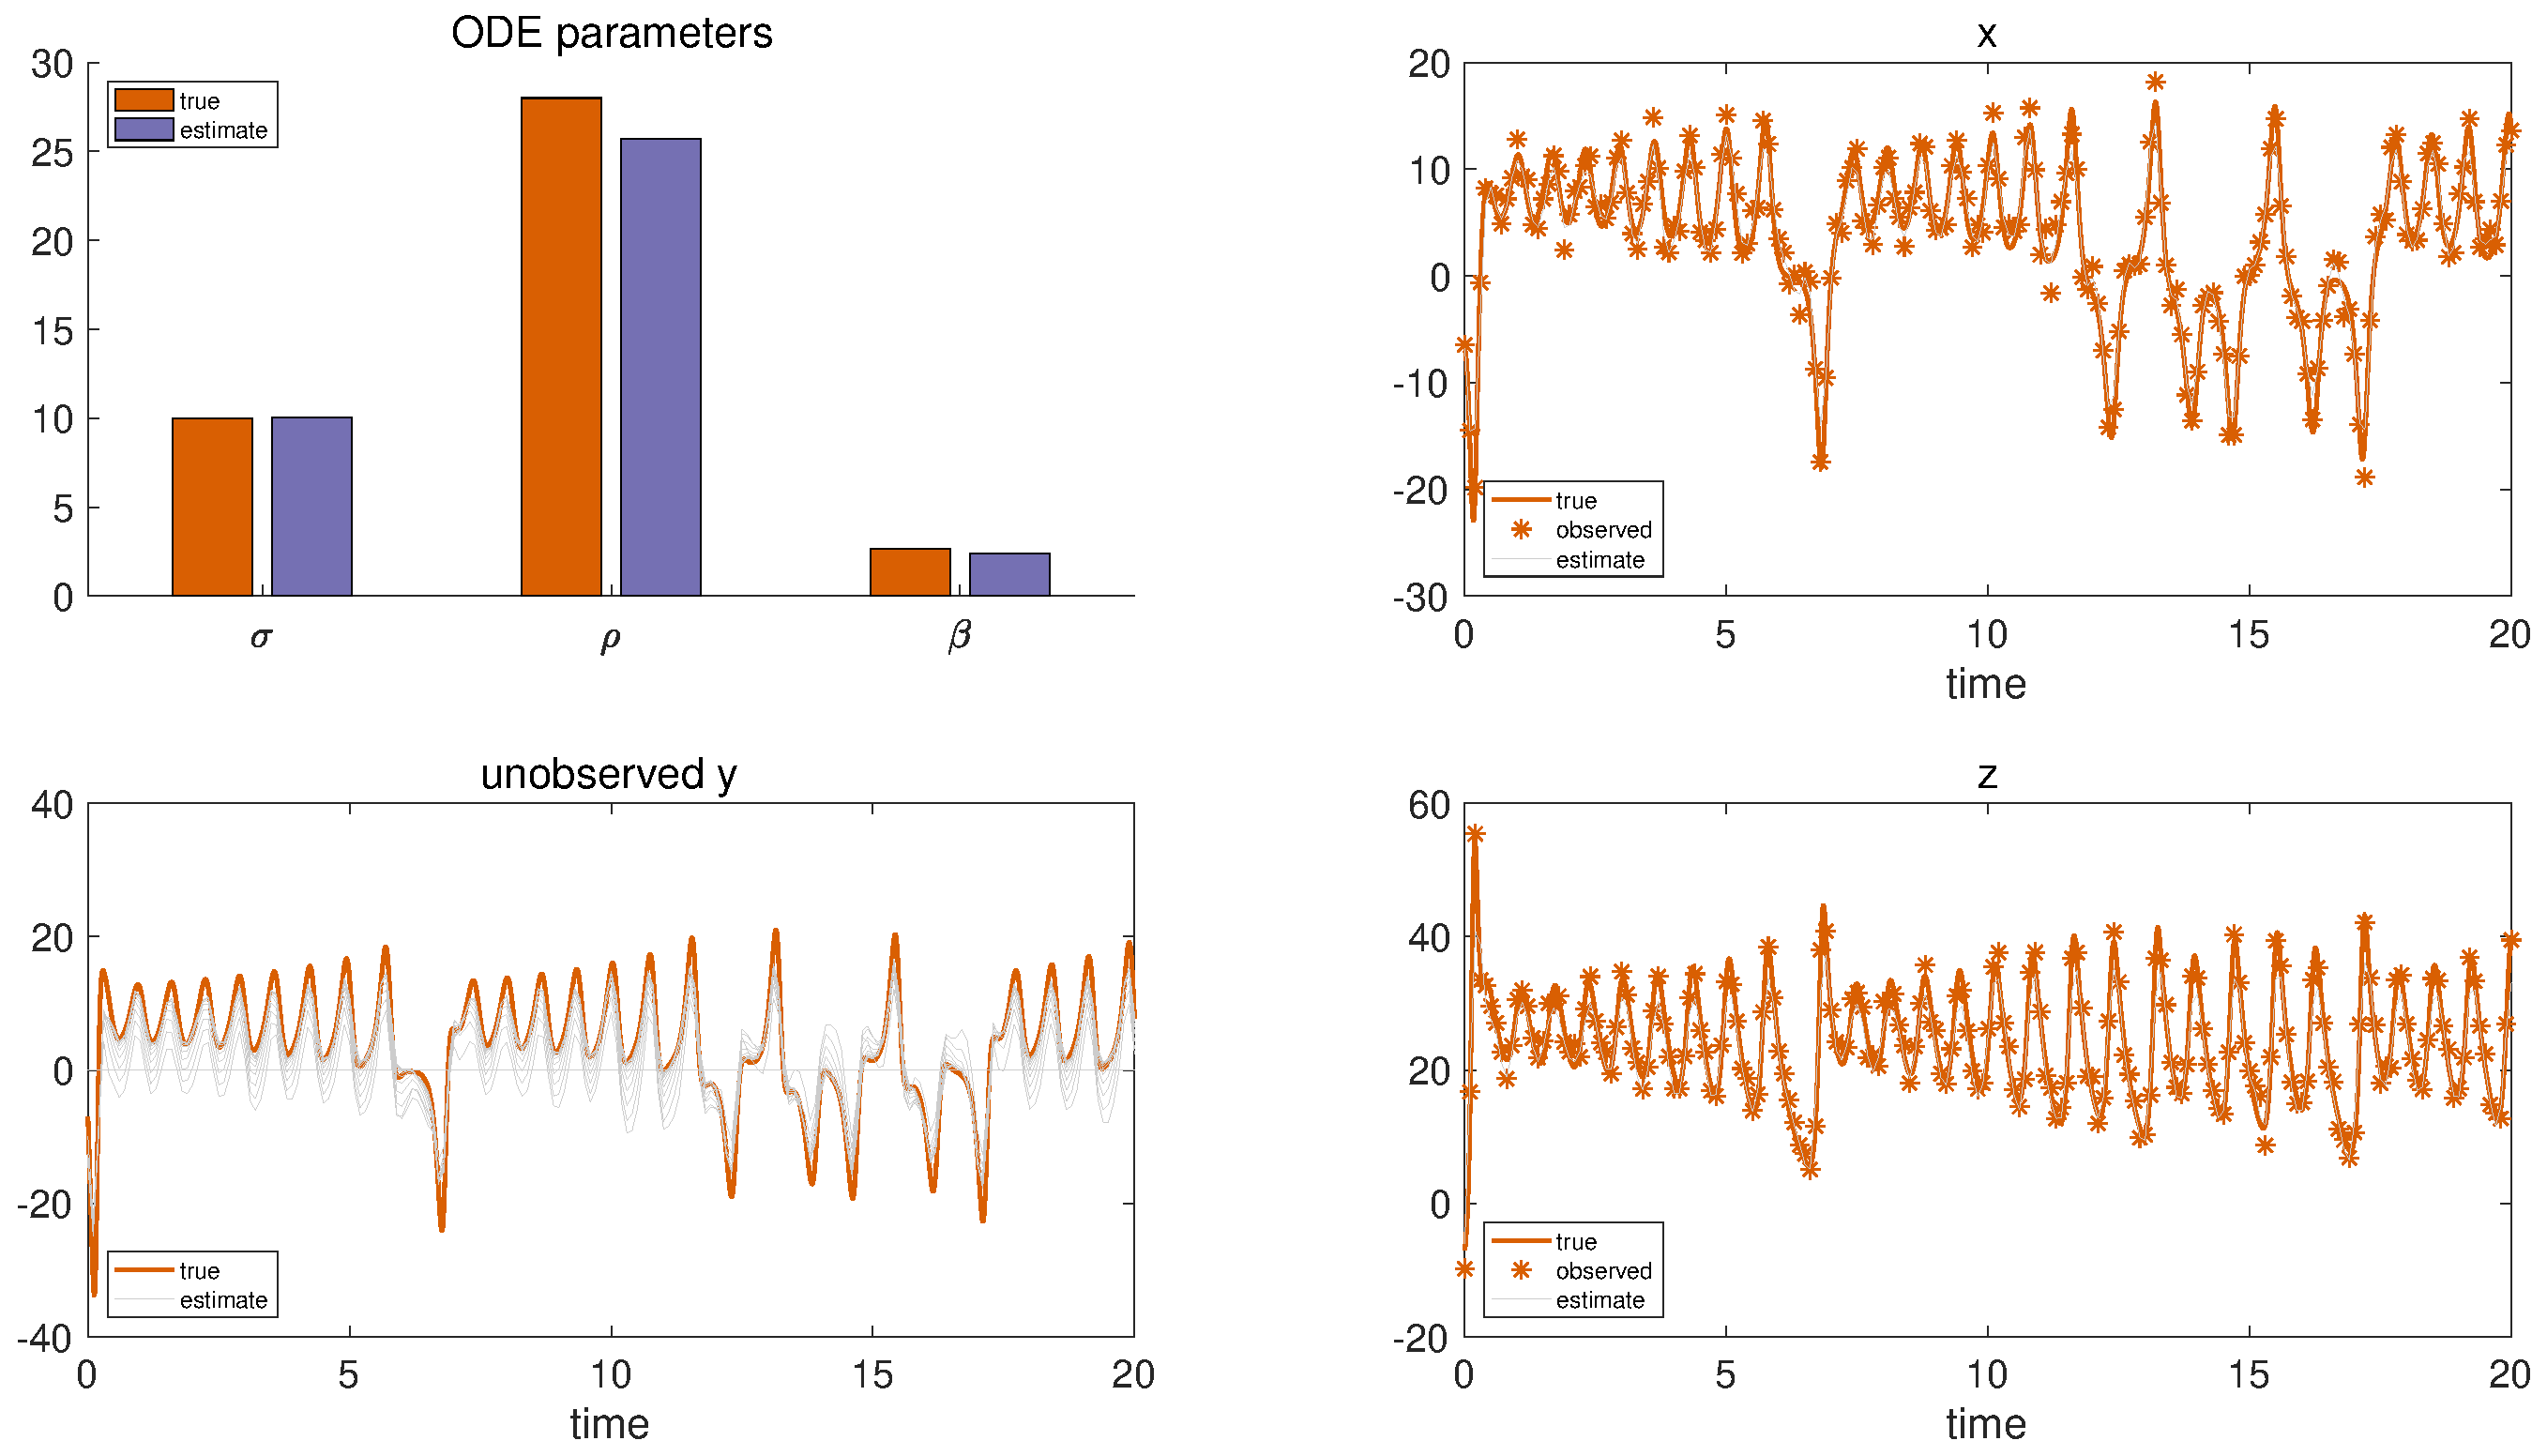
\includegraphics [width=5in]{Lorenz_attractor_4_40.eps}

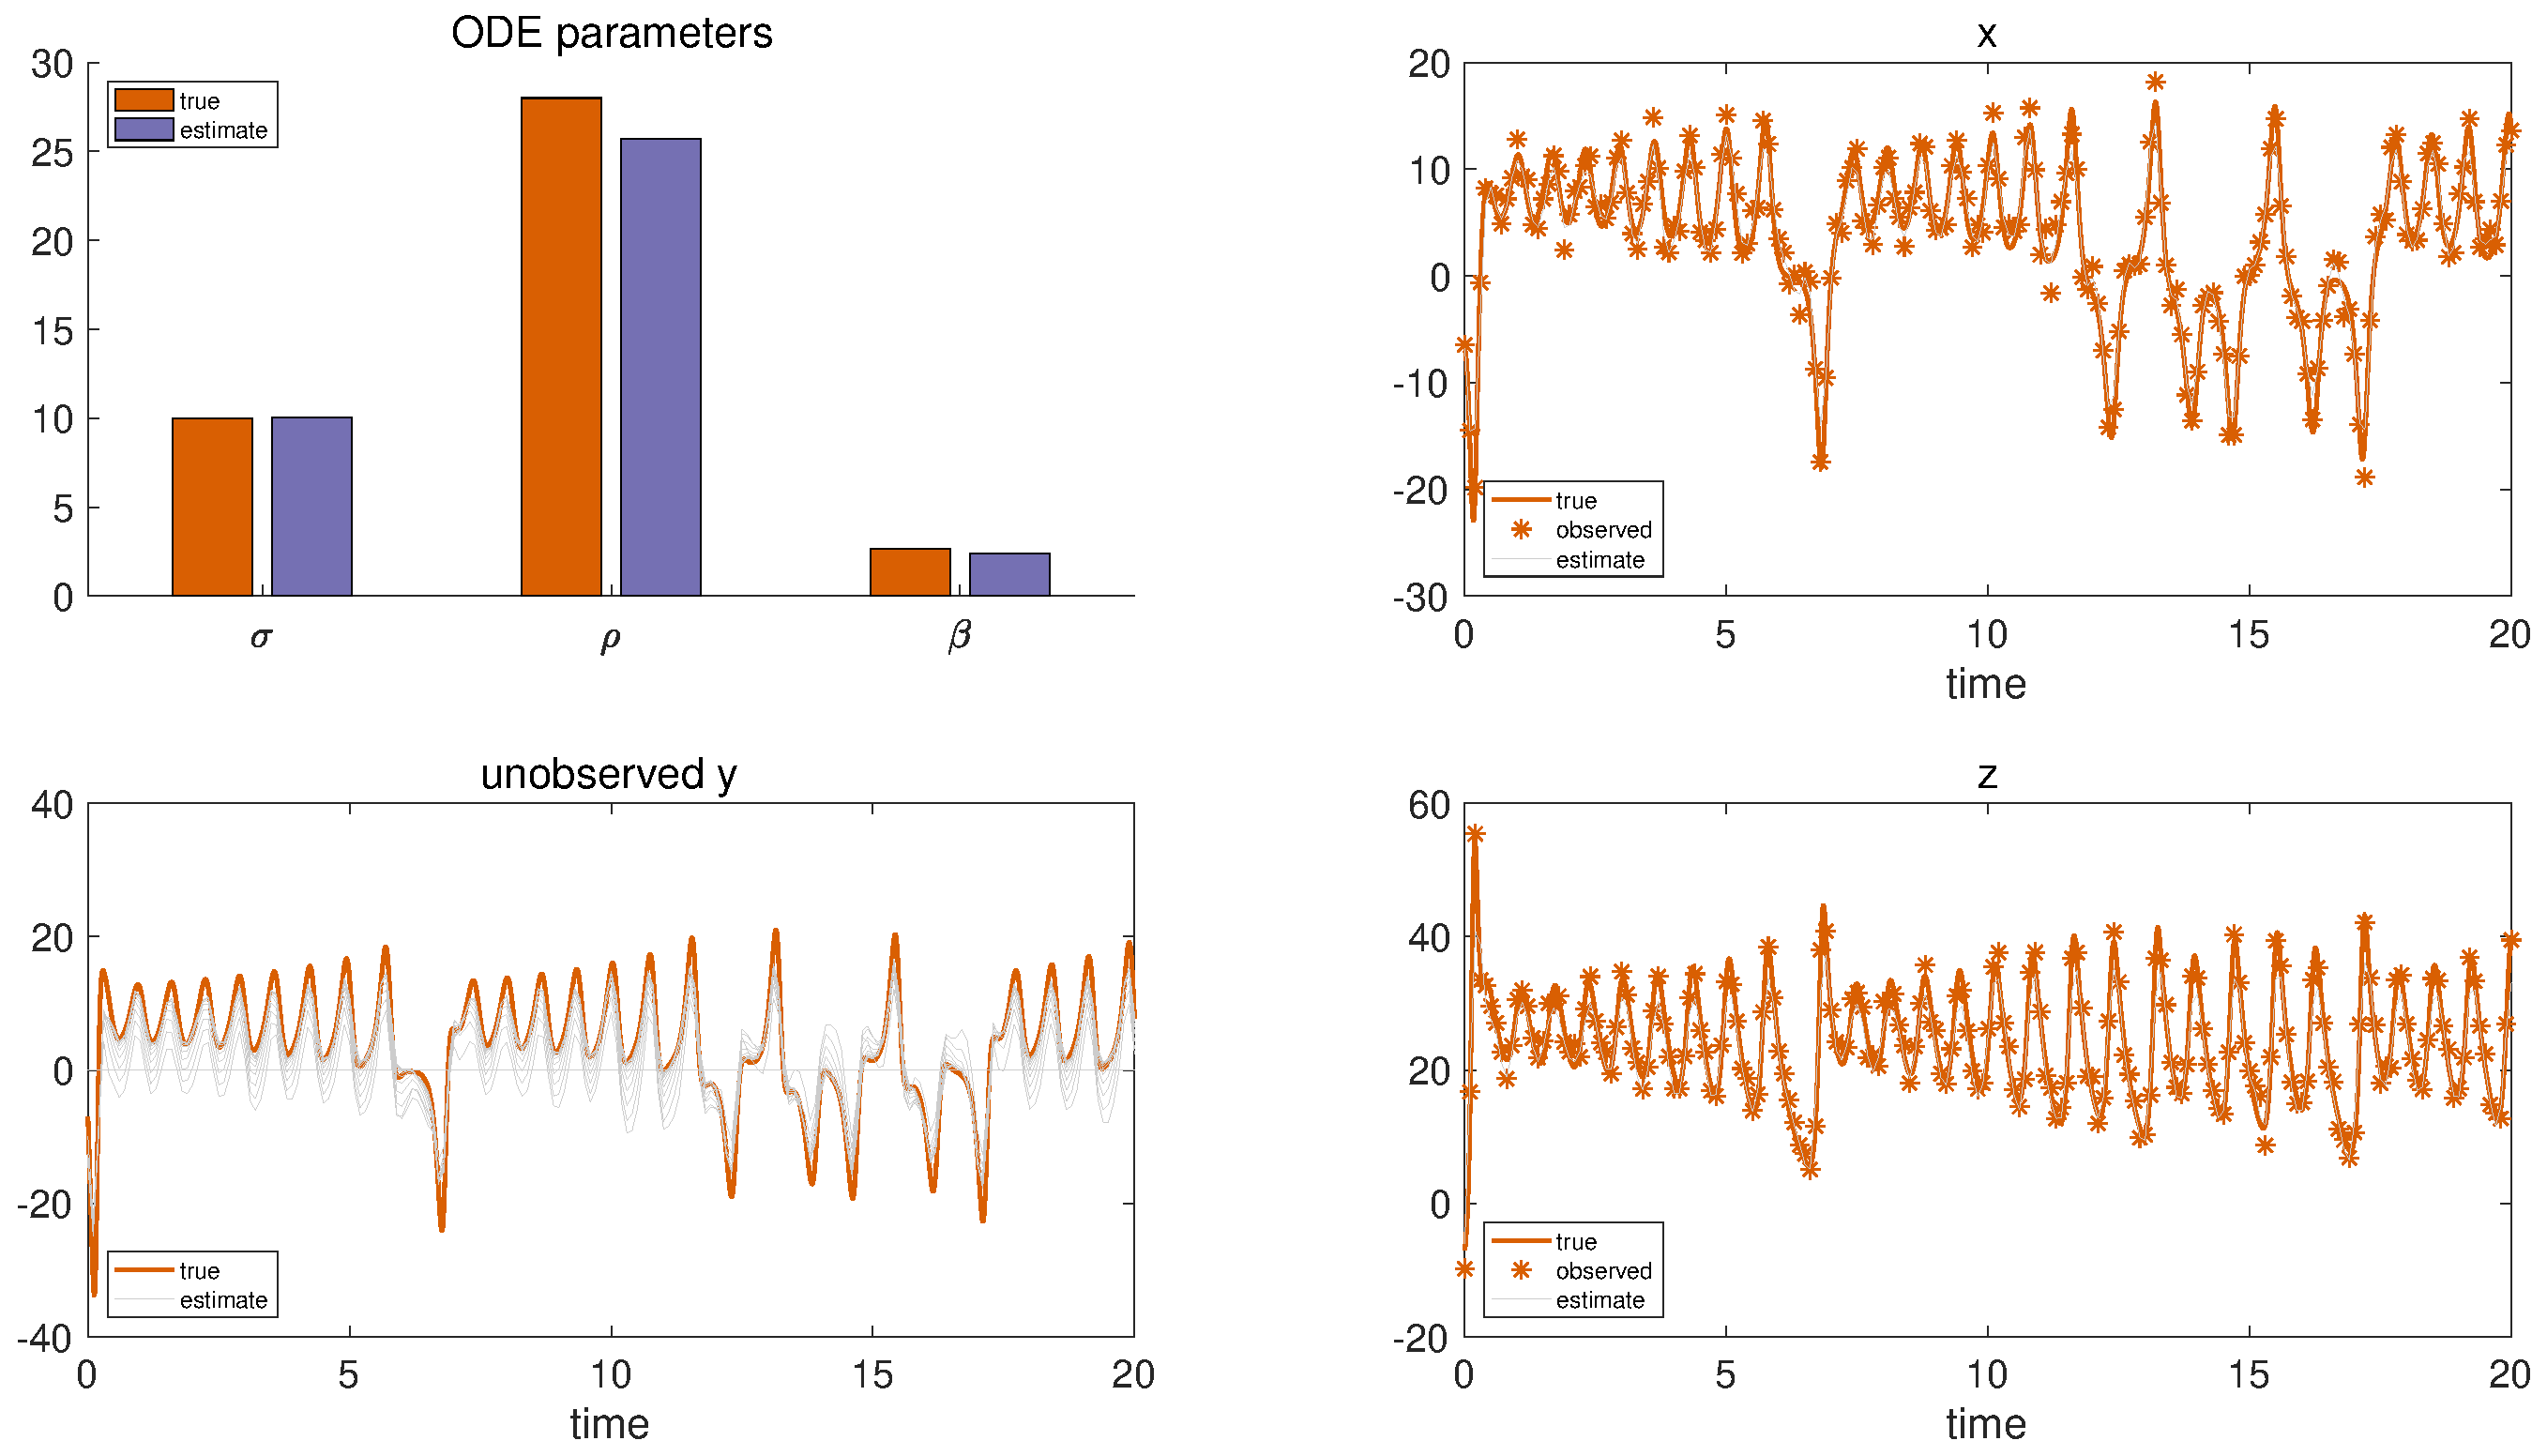
\includegraphics [width=5in]{Lorenz_attractor_4_41.eps}

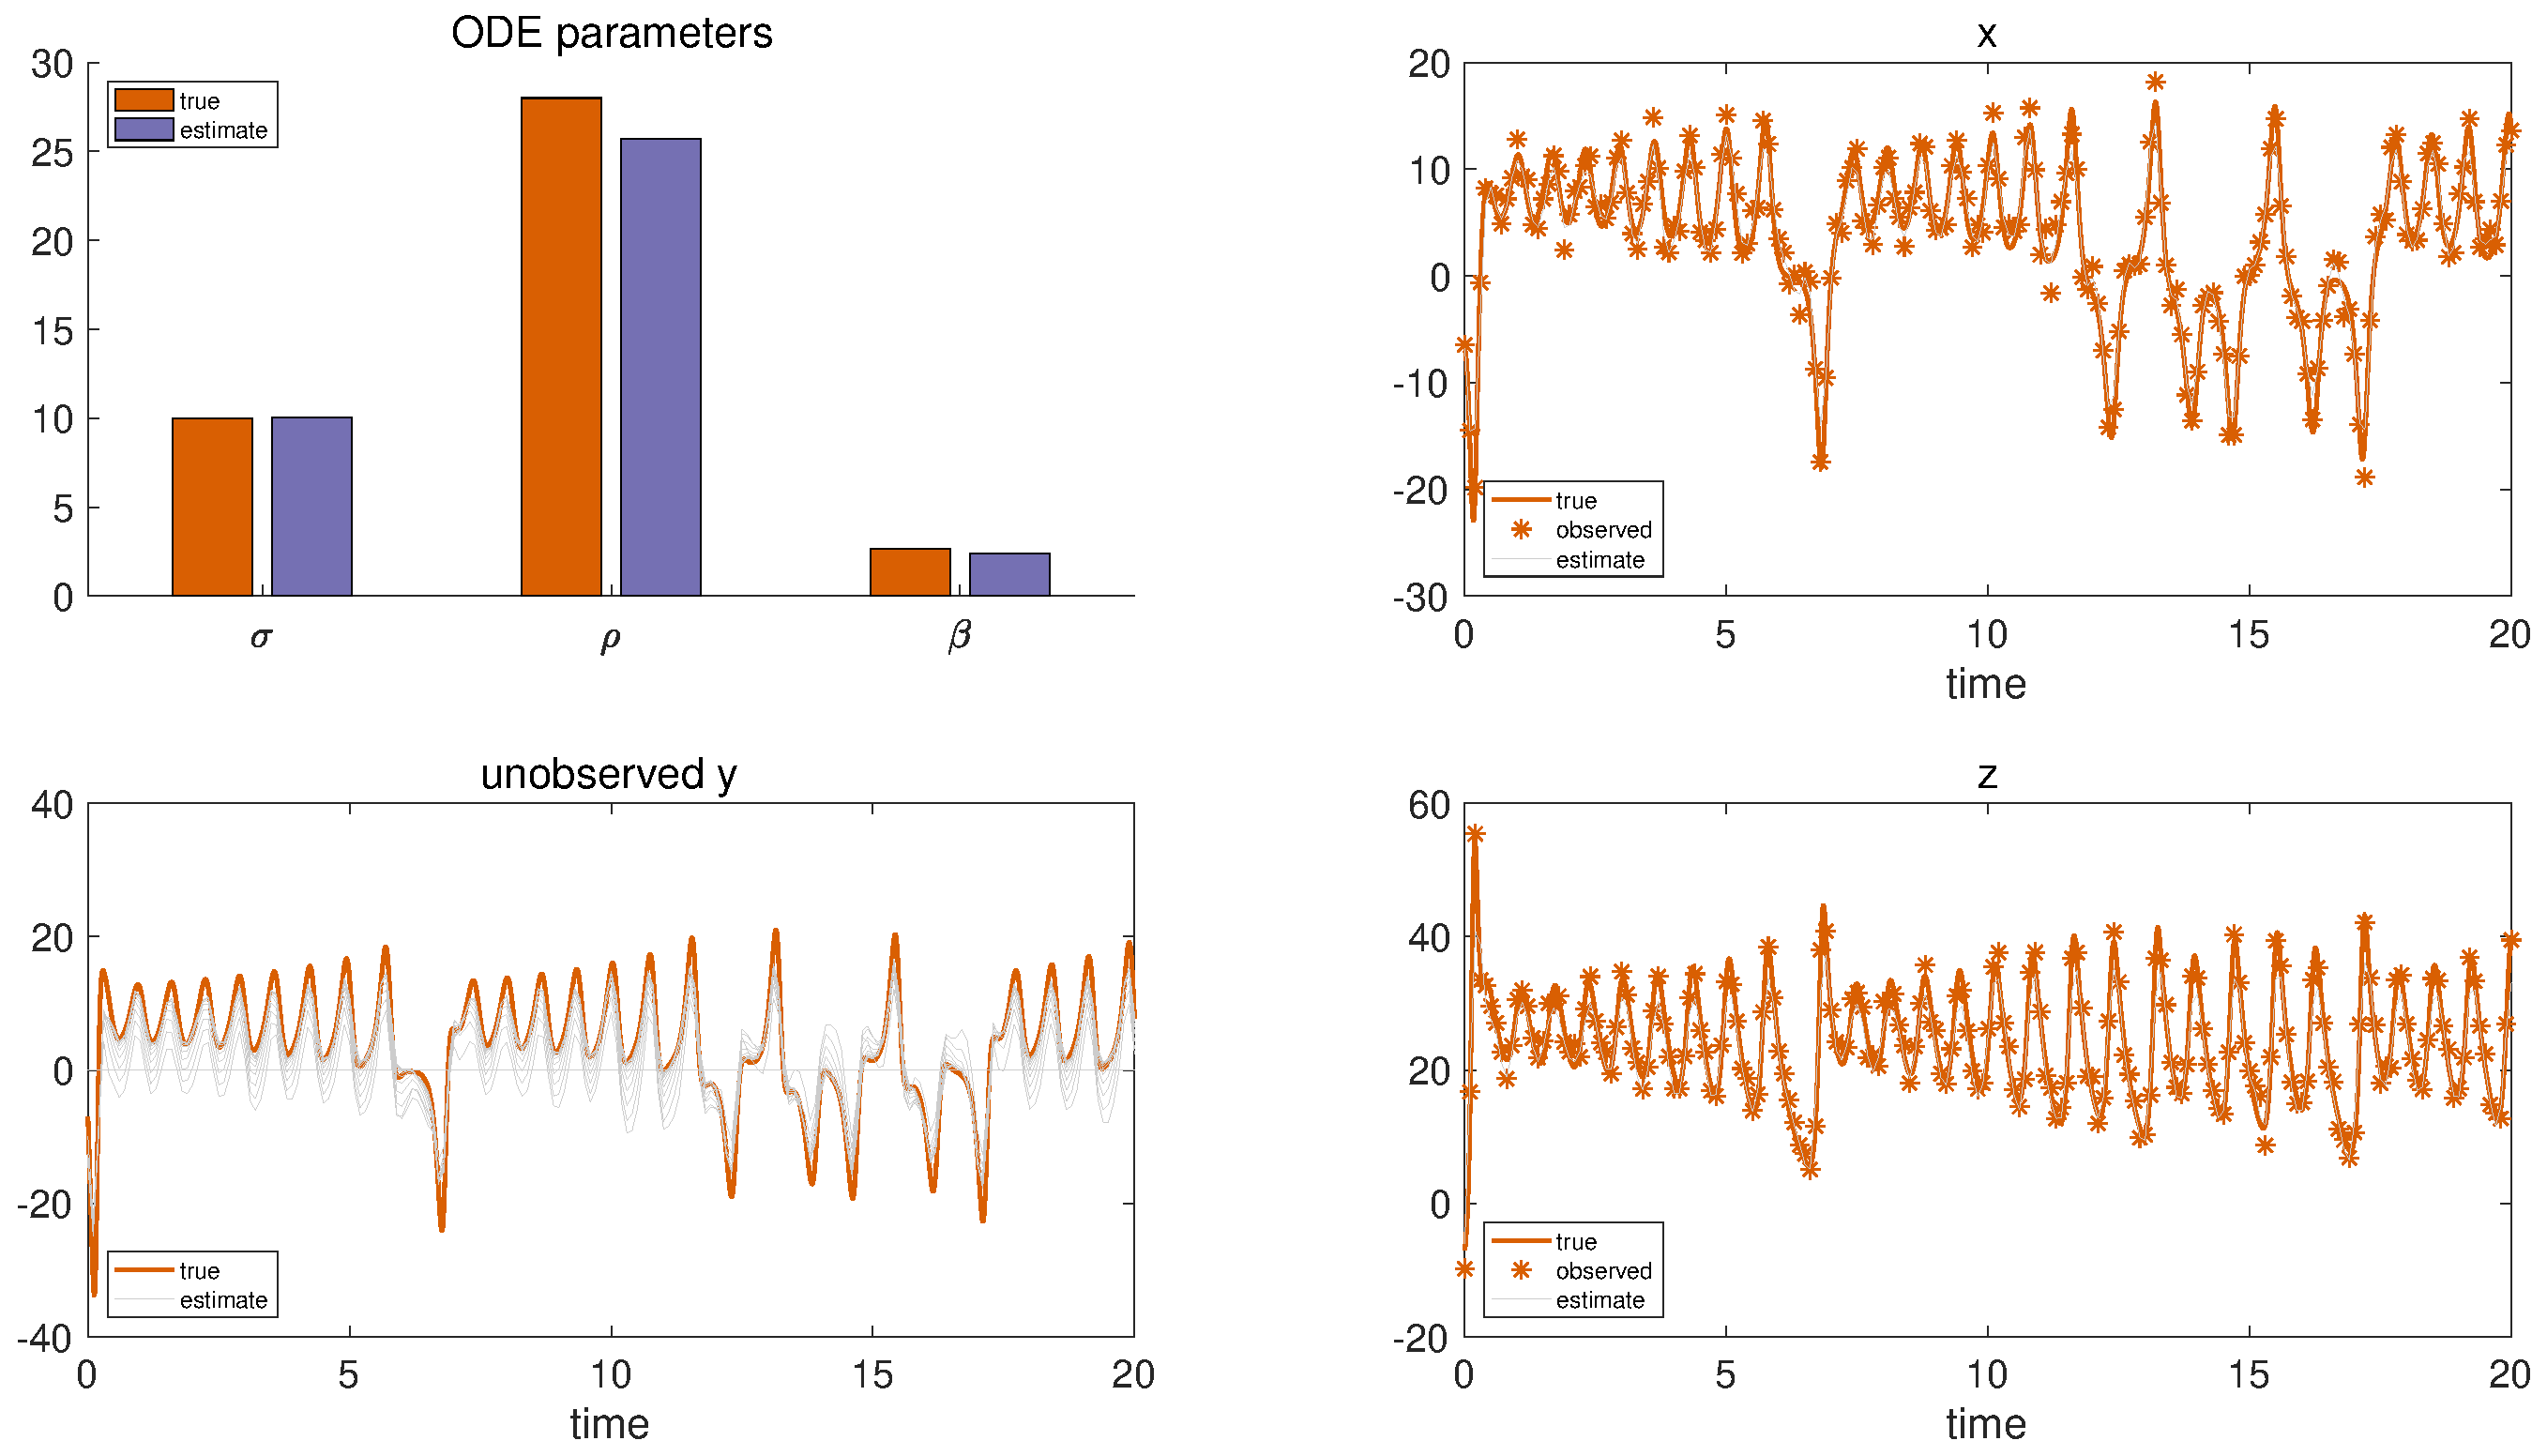
\includegraphics [width=5in]{Lorenz_attractor_4_42.eps}

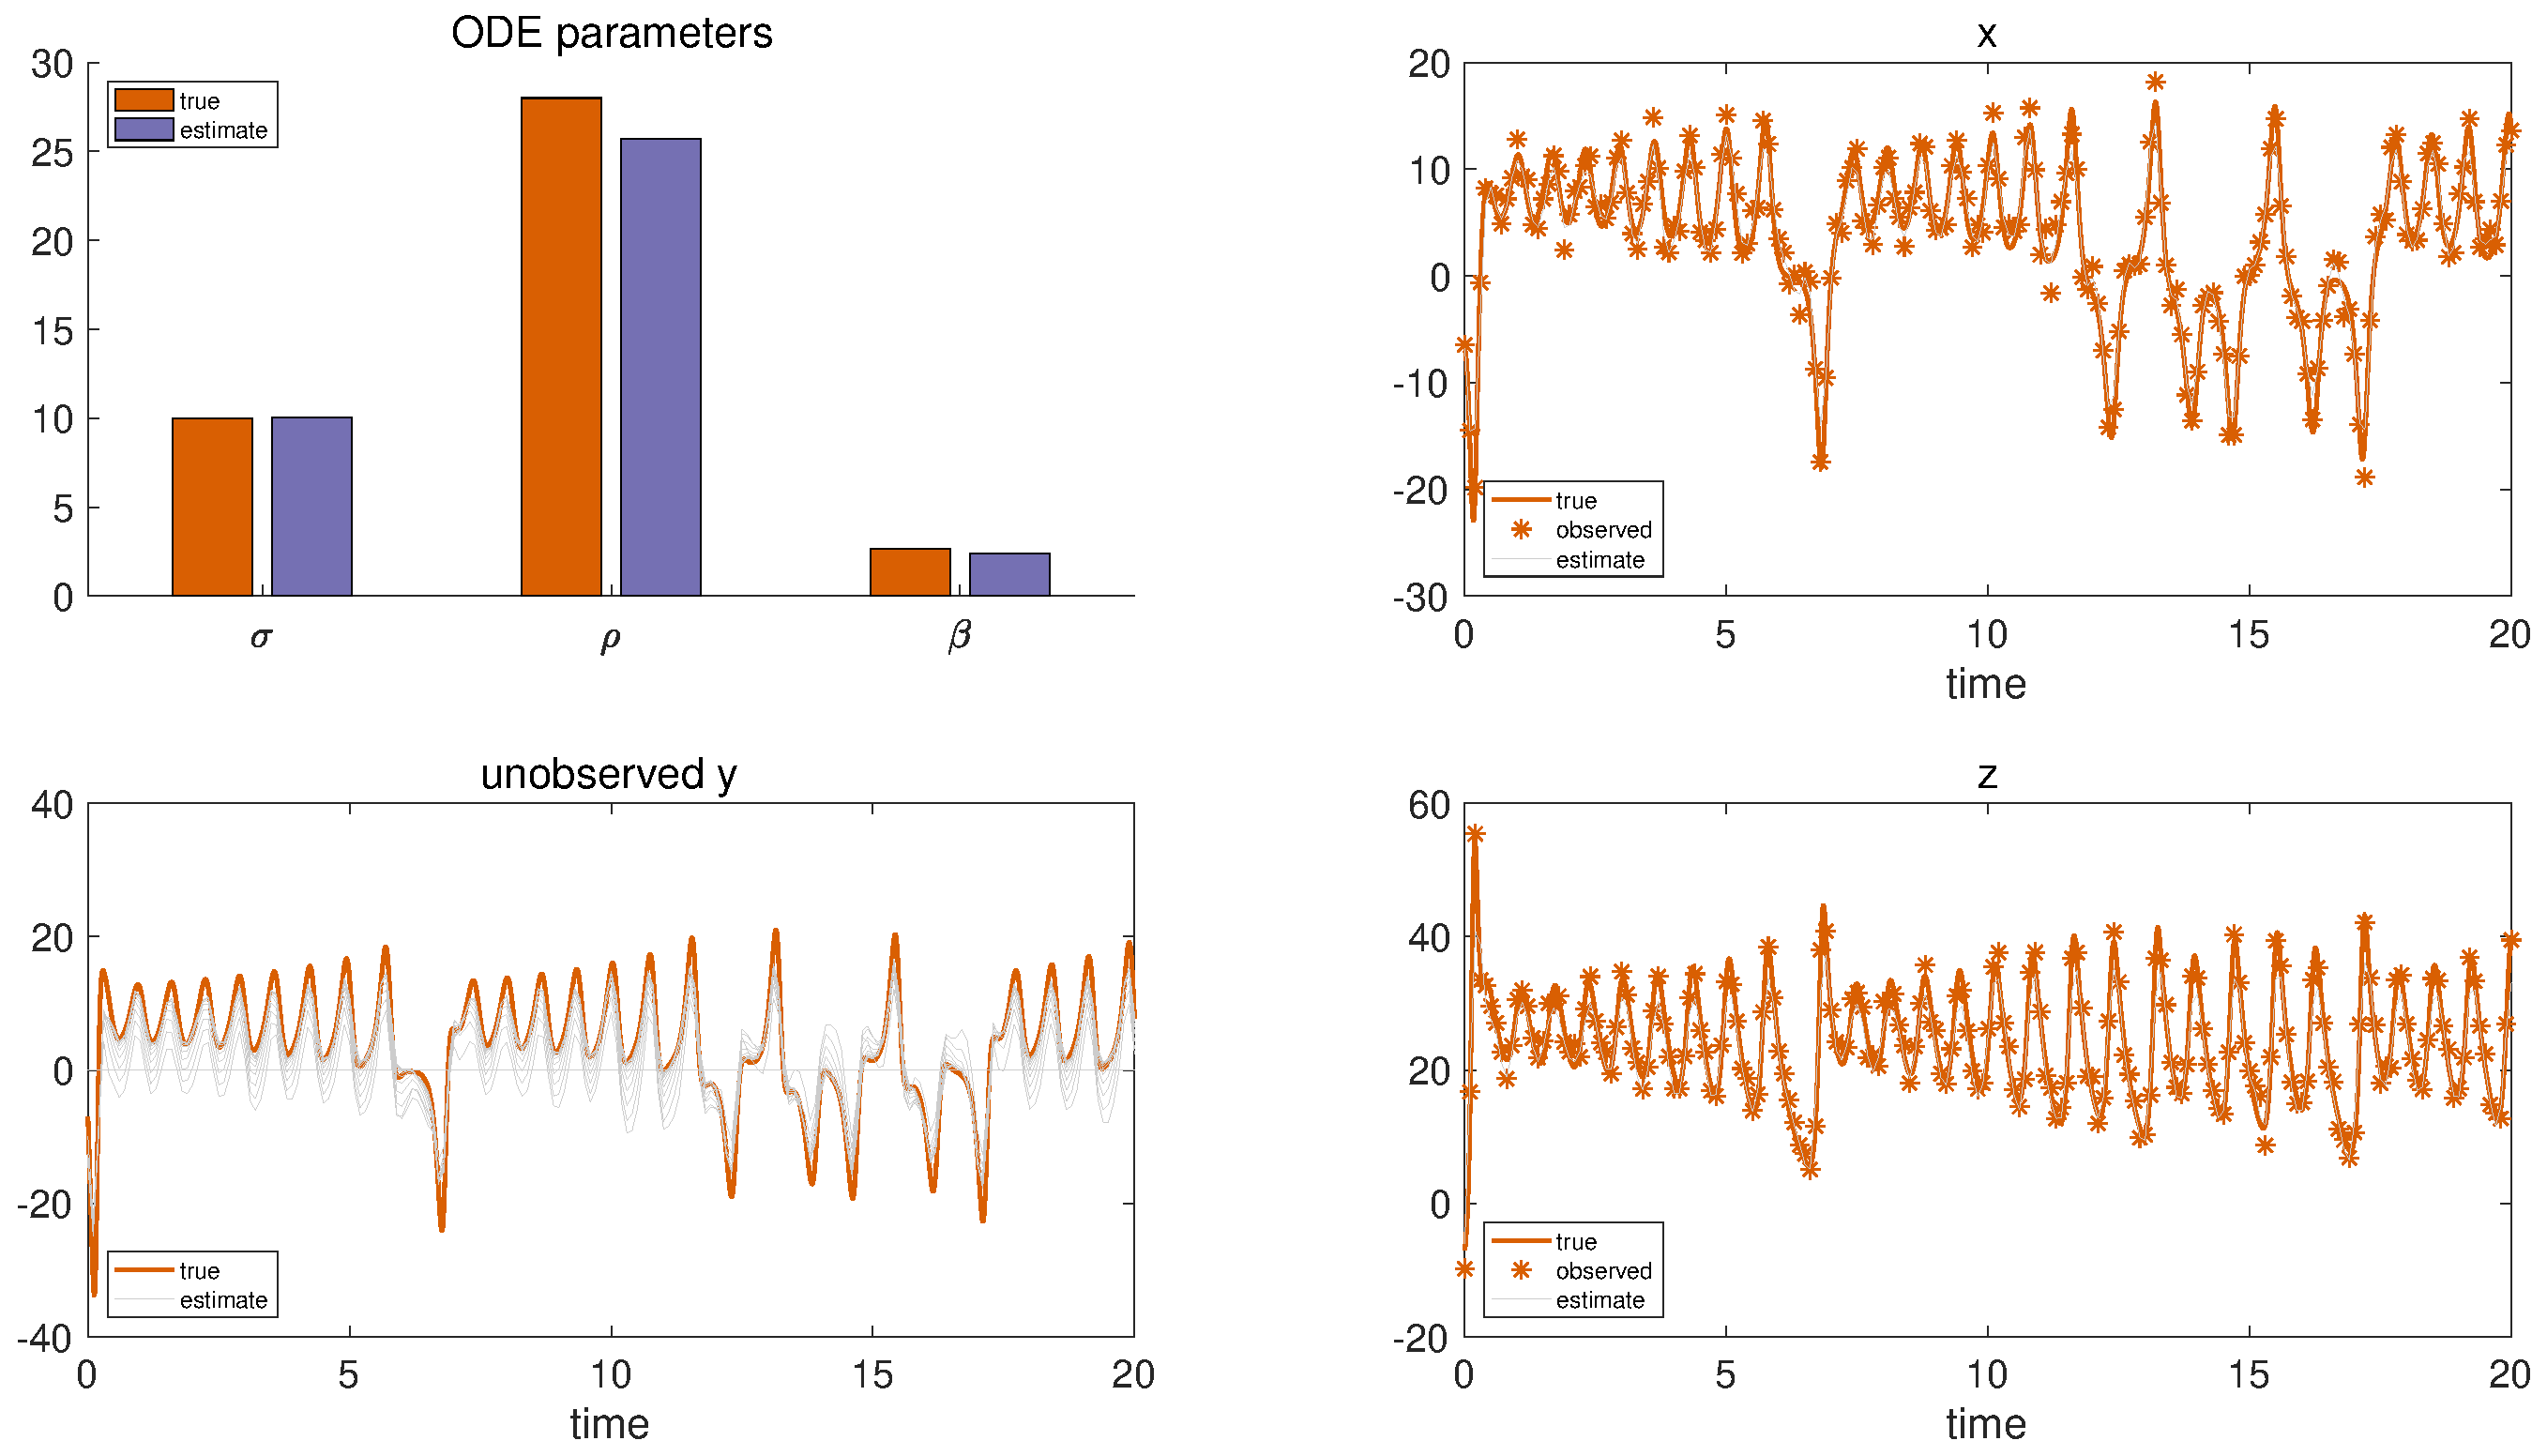
\includegraphics [width=5in]{Lorenz_attractor_4_43.eps}

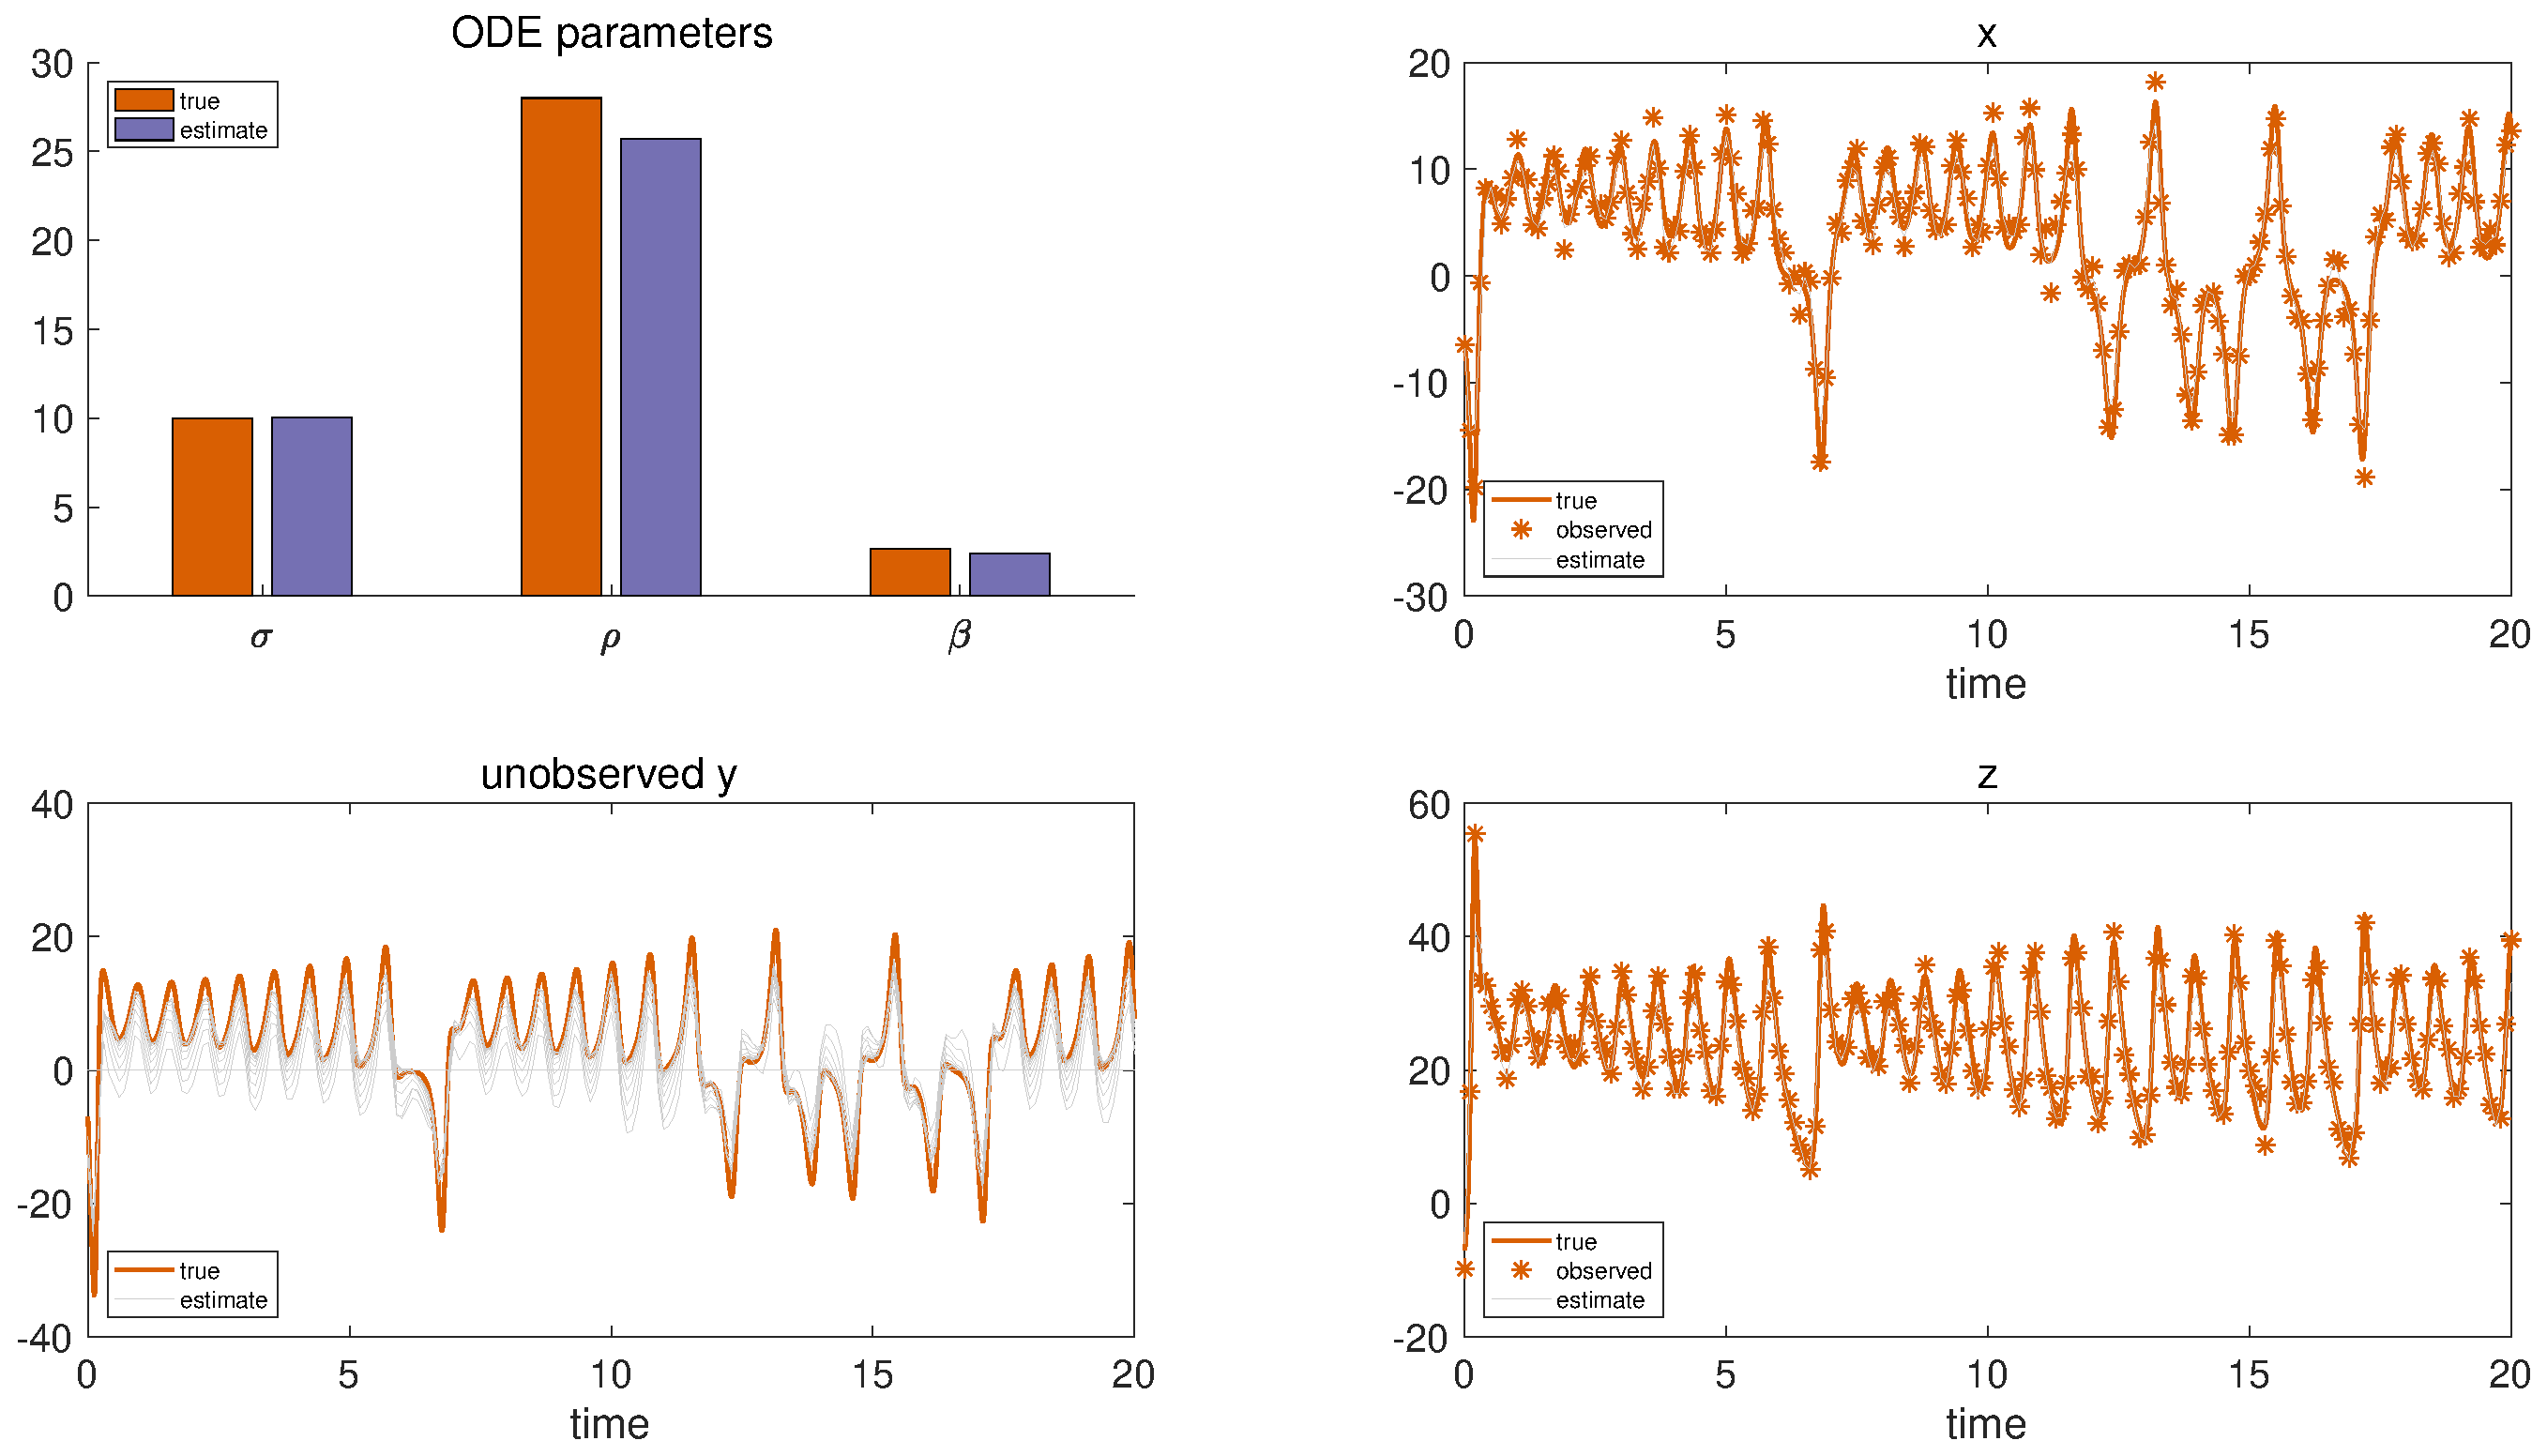
\includegraphics [width=5in]{Lorenz_attractor_4_44.eps}
}

\subsection{ Proxy for individual states }

\color{RoyalPurple}\begin{verbatim}
    [state.proxy.mean,state.proxy.inv_cov] = proxy_for_ind_states(state.lin_comb,...
        state.proxy.mean,param_proxy_mean',dC_times_invC,coupling_idx.states,symbols,...
        mu,inv_sigma,simulation.observed_states,A_plus_gamma_inv,opt_settings);
\end{verbatim}
\color{black}
\color{RoyalPurple}\begin{verbatim}
end
\end{verbatim}
\color{black}
\begin{par}
\subsection{ Final result }
\end{par} \vspace{1em}
\color{RoyalPurple}\begin{verbatim}
plot_results(h_states,h_param,state,time,simulation,param_proxy_mean,p,symbols,'final');
\end{verbatim}
\color{black}

\begin{figure}[tbh!]
\centering
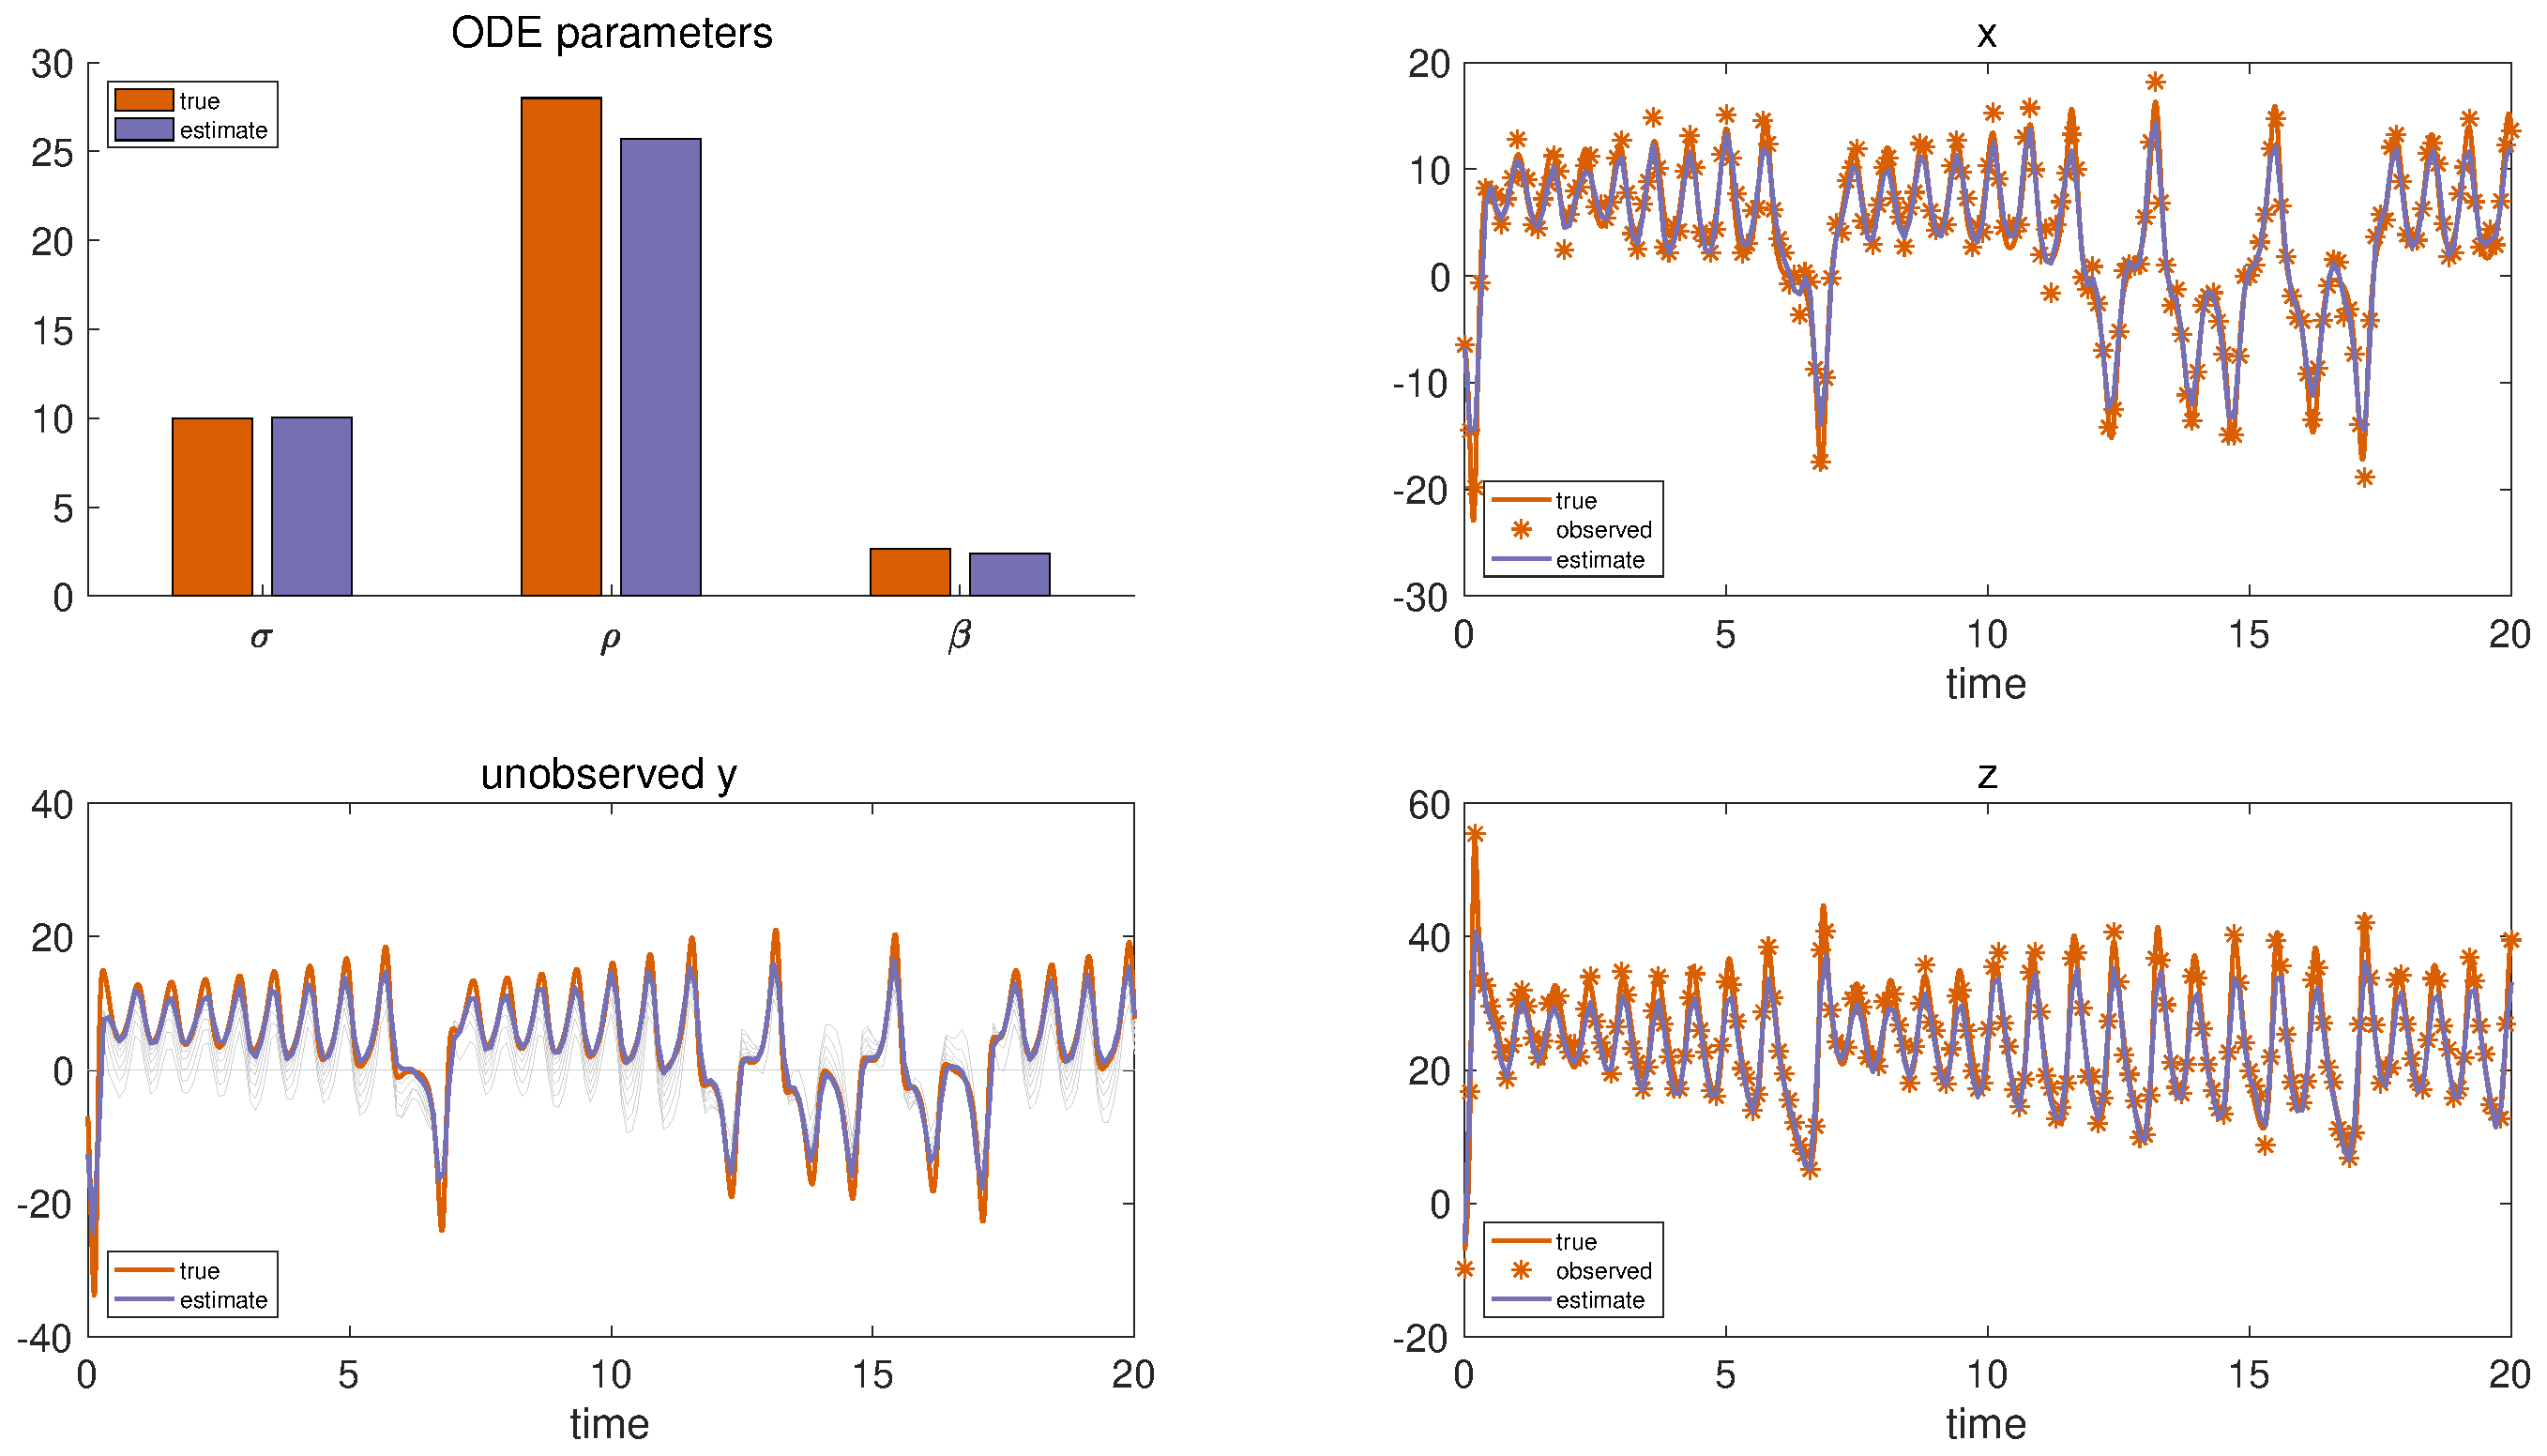
\includegraphics [width=5in]{Lorenz_attractor_4_45.eps}
\end{figure}

\section{Time Taken}

\color{RoyalPurple}\begin{verbatim}
disp(['time taken: ' num2str(toc) ' seconds'])
\end{verbatim}
\color{black}

        \begin{verbatim}time taken: 71.0552 seconds
\end{verbatim}
\color{black}
   